\documentclass[10pt]{book}
\usepackage[spanish]{babel}
\usepackage[utf8]{inputenc}
\usepackage[T1]{fontenc}
\usepackage{amsmath}
\usepackage{amsfonts}
\usepackage{amssymb}
\usepackage[version=4]{mhchem}
\usepackage{stmaryrd}
\usepackage{bbold}
\usepackage{graphicx}
\usepackage[export]{adjustbox}
\graphicspath{ {./images/} }
\usepackage{caption}

\title{ELEMENTOS DE CÁLCULO NUMÉRICO }

\author{Ricardo G. Durán, Silvia B. Lassalle y Julio D. Rossi}
\date{}


\begin{document}
\maketitle
\captionsetup{singlelinecheck=false}

\tableofcontents
\cleardoublepage


\chapter{Punto flotante y redondeo}
El objeto de este capítulo es analizar la representación de los números en una computadora y la propagación de los errores de redondeo al realizar cálculos.

Como la cantidad de información que puede guardarse en una computadora es finita, la máquina trabajará sólo con un conjunto finito de números. A estos los llamaremos números de máquina. En consecuencia, toda vez que de nuestros datos o cálculos surja un número que no pertenece a este conjunto finito, éste deberá ser reemplazado por una aproximación (el número de máquina más cercano). Este reemplazo da lugar a lo que llamamos errores de redondeo.

Al realizar cálculos estos errores de redondeo se propagan y esto puede llevar a resultados totalmente incorrectos como veremos en algunos ejemplos simples.

En las aplicaciones del cálculo numérico es prácticamente imposible determinar exactamente la magnitud de los errores de redondeo. Lo que si puede hacerse, y es de fundamental importancia, es identificar las posibles causas de que los errores se propaguen más de lo admisible. Esto permite mejorar los algoritmos o determinar que método es más conveniente para resolver un problema. Un claro ejemplo de esto, que veremos más adelante, aparece cuando se utiliza el método de eliminación de Gauss para resolver un sistema de ecuaciones lineales. En este caso, el análisis de la propagación de errores permite determinar la forma más eficiente de aplicar el método.

Por otra parte, es fundamental distinguir cuando la propagación excesiva de errores se debe a que el algoritmo utilizado es "malo" o inestable o a que el problema en sí mismo está "mal condicionado". En el primer caso se puede (se debe!) tratar de mejorar el método de resolución mientras que en el segundo caso el problema es más esencial. Los ejemplos que presentaremos ilustrarán estos dos casos.

\section{Punto flotante}
En lo que sigue supondremos que los números de máquina son los que aparecen en la pantalla. Esto no es exacto pues en realidad la computadora opera internamente con los números desarrollados en base 2 y no en base 10. Este abuso de lenguaje es sólo para mayor claridad (el lector podrá observar que todo nuestro análisis puede repetirse trabajando en base 2).

Observemos primero que un número real cualquiera, $x \in \mathbb{R}, x>0$, puede escribirse como

$$
x=0, a_{1} a_{2} \ldots a_{k} \ldots 10^{l}=r \times 10^{l}, \quad \frac{1}{10} \leq r<1 \quad\left(\text { es decir }, a_{1} \neq 0\right)
$$

Pero en una computadora no se pueden poner infinitos dígitos. Por lo tanto, se trabaja sólo con números de desarrollo finito y de una longitud dada. De la misma forma, el exponente $l$ (es decir el orden del número) estará limitado a cierto rango. En consecuencia los números de máquina serán de la forma

$$
x=0, a_{1} a_{2} \ldots a_{m} 10^{l}=q \times 10^{l} \quad-M_{1} \leq l \leq M_{2},, a_{1} \neq 0
$$

más los correspondientes negativos y el cero. Los números $m, M_{1}$ y $M_{2}$ dependen de la máquina. Esta representación de los números es la que se llama de punto flotante.

Los números de máquina forman un conjunto finito de números racionales. La cantidad de números de máquina que hay entre $1 / 10$ y 1 es ,

$$
\#\{x / 1 / 10 \leq x<1\}=9 \times 10^{m-1} .
$$

En general, la cantidad que hay entre $10^{l}$ y $10^{l+1}$ es también $9 \times 10^{m-1}$. Esto nos dice que los números de máquina no están uniformemente distribuidos. Sí lo está el subconjunto que está entre $10^{l}$ y $10^{l+1}$ para cada $l$. En particular, los números más grandes están más separados. Resulta útil para la comprensión hacer un dibujo de los números de máquina en la recta numérica (Ejercicio). Al analizar la propagación de errores de redondeo se aclarará por qué esta distribución de los números es más razonable que una uniforme.

Sea $x \in \mathbb{R}$. Para simplificar notación supondremos $x>0$ (claramente todas las consideraciones que haremos se aplican análogamente a los números negativos). Hay dos posibilidades: que $x$ esté o no en el rango de los números de máquina. Si al hacer cálculos aparece un número en la segunda situación, por ser muy grande o muy chico, la computadora nos dará un mensaje indicándolo.

Supongamos entonces que $x$ está en el rango de la máquina, o sea,

$$
x=0, a_{1} a_{2} \ldots a_{m} \ldots 10^{l} \quad M_{1} \leq l \leq M_{2}, a_{1} \neq 0
$$

Este $x$ está entre dos números de máquina,

$$
x^{\prime} \leq x \leq x^{\prime \prime}
$$

Supongamos, para simplificar, que $a_{m} \neq 9$ (analice el lector el caso contrario). Entonces tenemos

$$
x^{\prime}=0, a_{1} a_{2} \ldots a_{m} 10^{l}
$$

y

$$
x^{\prime \prime}=0, a_{1} a_{2} \ldots\left(a_{m}+1\right) 10^{l}
$$

\section{Redondeo}
Hay dos formas de aproximar a $x$. Una es por truncamiento: se elige siempre $x^{\prime}$ es decir el mayor de los números de máquina que son menores que $x$. La otra forma es tomar el más próximo a $x$ entre $x^{\prime}$ y $x^{\prime \prime}$. A esta forma de aproximar se la conoce por redondeo y es la que usan habitualmente las computadoras.

Veamos que error cometemos al aproximar un número por redondeo. Usaremos la notación

$$
x^{*}=x \quad \text { redondeado }
$$

El error absoluto será

$$
\left|x-x^{*}\right| \leq \frac{1}{2} \frac{1}{10^{m}} 10^{l}
$$

Mientras que el error relativo se puede acotar de la forma siguiente

$$
\frac{\left|x-x^{*}\right|}{|x|} \leq \frac{1}{2} \frac{10^{l-m}}{0, a_{1} a_{2} \ldots a_{m} \ldots 10^{l}}
$$

y como

$$
0, a_{1} a_{2} \ldots a_{m} \ldots \geq \frac{1}{10}
$$

se tiene que

$$
\frac{\left|x-x^{*}\right|}{|x|} \leq 5 \times 10^{-m}
$$

Es decir que el error relativo es del orden de $10^{-m}$ si nuestra máquina trabaja con $m$ dígitos.\\
Es importante observar que, si bien el error absoluto que introduce el redondeo depende de la magnitud del número, el relativo, que es el más significativo, es independiente de ésta, está controlado en términos de la cantidad de dígitos con la que trabaja nuestra computadora (Ejercicio: meditar que tiene que ver esto con la distribución no uniforme de los números de máquina).

Si tenemos

$$
x^{*}=0, a_{1} a_{2} \ldots a_{m} 10^{l}, \quad a_{1} \neq 0
$$

decimos que conocemos a $x$ con $m$ dígitos significativos, lo que equivale, según vimos, a conocerlo con un error relativo del orden de $10^{-m}$. Observar la importancia de la condición $a_{1} \neq 0$ : de lo contrario los dígitos dejan de ser significativos.

Observemos que

$$
x^{*}=x(1+\delta)
$$

con

$$
|\delta| \leq \varepsilon=5 \times 10^{-m}
$$

Este $\varepsilon$ es el error de redondeo unitario, es decir, que el error que se comete al aproximar $x$ por $x^{*}$ es $x \delta$ con $|\delta| \leq \varepsilon$, de esta forma el error $\left|x-x^{*}\right|$ será menor o igual que $\varepsilon|x|$.

Este valor, $\varepsilon$, depende de la máquina y se lo llama el $\varepsilon$ de la máquina. Recordemos que, según lo comentado antes, el verdadero $\varepsilon$ de máquina no es exactamente éste debido a que la computadora trabaja en base 2 . Pero desde el punto de vista práctico sólo interesa el orden de $\varepsilon$ (y éste sí es correcto!).

Ejercicio: calcular el $\varepsilon$ exacto suponiendo que la máquina trabaja en base 2 con $k$ dígitos.

Otra forma de interpretar el significado del $\varepsilon$ de la máquina es la siguiente: $\varepsilon$ nos dice cuál es el menor número tal que, en la máquina,

$$
1+\varepsilon \neq 1
$$

O sea, si se le suma a 1 algo menor que $\varepsilon$, "desaparece" debido al redondeo. En efecto, según la máquina tendremos

$$
1+4 \times 10^{-m}=1,0 \ldots 04=0,10 \ldots 00 \times 10=1
$$

en cambio,

$$
1+\varepsilon=1,0 \ldots 06=0,10 \ldots 01 \times 10 \neq 1
$$

Si sumamos exactamente $\varepsilon$ el resultado dependerá de como redondee la máquina en el caso en que $x$ equidista de dos números de máquina, es decir, cuando la cifra $m+1$ es justo 5 .

Más en general, el orden del menor número que sumado a un $x$ da, en la máquina, un resultado distinto de $x$ es $\varepsilon|x|$.

Es fundamental observar que $\varepsilon$ no es el menor número que se puede representar en la máquina (y está muy lejos de éste!). Este último depende de $M_{1}$ y no de $m$.

Veamos ahora algunos de los problemas que surgen debido al redondeo.\\
Empecemos por sumar dos números. Como vimos, si sumamos dos números de ordenes muy distintos, el más chico puede "desaparecer". Por ejemplo, si $m=5$ y

$$
x=78473000 ; \quad y=24
$$

tenemos

$$
x^{*}=0,78473 \times 10^{8} ; \quad y^{*}=0,24 \times 10^{2}
$$

es decir que $x$ e $y$ son números de máquina. Entonces,

$$
x+y=78473024
$$

y por lo tanto,

$$
(x+y)^{*}=0,78473 \times 10^{8}=x^{*}=x
$$

En particular, esto nos dice que si tenemos que sumar varios números $x_{1}, x_{2}, \ldots, x_{N}$ conviene hacerlo de menor a mayor (¿Por qué?).

En el ejemplo anterior el problema no es muy importante ya que no se pierden dígitos significativos, es decir, el orden del error relativo no se agranda (se está perdiendo la información de un número que es despreciable respecto del otro sumando).

El problema es mucho más serio cuando deben restarse dos números parecidos. En este caso, debido a lo que se conoce como "cancelación catastrófica", pueden perderse dígitos significativos o, en otras palabras, agrandarse mucho el error relativo.

Consideremos como antes $m=5$ y tomemos

$$
x=0,372154876 ; \quad y=0,372023264
$$

entonces,

$$
x^{*}=0,37215 ; \quad y^{*}=0,37202
$$

y por lo tanto,

$$
x-y=0,000131612
$$

mientras que

$$
x^{*}-y^{*}=0,00013=0,13 \times 10^{-3}
$$

Observemos qué sucedió: $x$ e $y$ estaban representados con 5 dígitos significativos pero al restarlos quedaron sólo 2 del resultado. En consecuencia el error relativo creció de manera tal que si bien el error relativo en $x$ e $y$ era del orden de $10^{-5}$ el del resultado es del orden de $10^{-2}$.

Como conclusión observamos que hay que tratar de evitar restar números "casi iguales". Por ejemplo, supongamos que queremos calcular

$$
y=\sqrt{x^{2}+1}-1
$$

para valores de $x$ pequeños. Si lo hacemos directamente, estamos en la situación anterior. En cambio podemos proceder de la siguiente manera:

$$
y=\sqrt{x^{2}+1}-1=\frac{\left(\sqrt{x^{2}+1}-1\right)\left(\sqrt{x^{2}+1}+1\right)}{\left(\sqrt{x^{2}+1}+1\right)}=\frac{x^{2}}{\left(\sqrt{x^{2}+1}+1\right)}
$$

y utilizar la última expresión para calcular $y$. Si los cálculos fueran exactos ambas fórmulas darían el mismo resultado pero, debido al redondeo, dan resultados distintos. Por ejemplo, trabajando con 5 dígitos, si $x=0,0312$ obtenemos con la primera fórmula $y=0,0004$ (un solo dígito significativo si bien conocíamos $x$ exactamente). Mientras que con la segunda, $y=0,00048662$ (que tiene cuatro dígitos significativos correctos).

El mismo problema surge al calcular $y=x-\operatorname{sen} x$ para $x$ pequeño. En este caso se puede usar el desarrollo de Taylor,

$$
y=x-\operatorname{sen} x=\frac{x^{3}}{3!}-\frac{x^{5}}{5!}+\frac{x^{7}}{7!} \ldots
$$

y calcular $y$ sumando los primeros términos de la serie.\\
Otro caso en el que la cancelación de dígitos significativos puede presentarse es en la resolución de una ecuación cuadrática

$$
a x^{2}+b x+c=0
$$

si utilizamos la fórmula habitual

$$
x_{1}=\frac{-b+\sqrt{b^{2}-4 a c}}{2 a} \quad \text { y } \quad x_{2}=\frac{-b-\sqrt{b^{2}-4 a c}}{2 a}
$$

Consideremos por ejemplo,

$$
x^{2}-10^{5} x+1=0
$$

Los primeros dígitos exactos de las raíces son

$$
x_{1}=99999,99999
$$

y

$$
x_{2}=0,000010000000001
$$

Usando la fórmula para $x_{2}$ tenemos

$$
x_{2}=\frac{10^{5}-\sqrt{10^{10}-4}}{2}
$$

Si trabajamos con ocho dígitos el 4 desaparece y $x_{2}$ resulta igual a cero. Otra vez hemos restado dos números parecidos!

Esto se puede solucionar calculando primero $x_{1}$ y luego obtener $x_{2}$ usando que $x_{2}=\frac{c}{a x_{1}}$.\\
En general, la forma correcta de encontrar las raíces en el caso en que $a c$ sea despreciable respecto de $b$, es calculando primero

$$
x_{1}=\frac{-b-\operatorname{sign}(b) \sqrt{b^{2}-4 a c}}{2 a}
$$

y luego la otra raiz como hicimos en el ejemplo. De esta forma se evita la pérdida de dígitos significativos.

Un problema fundamental del cálculo numérico es la resolución de sistemas de ecuaciones lineales. Veamos cómo los errores de redondeo pueden afectar la solución aún en problemas de dos ecuaciones con dos incógnitas. Tratemos de resolver el siguiente sistema utilizando el método de eliminación de Gauss,

$$
\left(\begin{array}{ll}
\varepsilon & 1 \\
1 & 1
\end{array}\right)\binom{x}{y}=\binom{1}{2}
$$

Pongamos, a modo de ejemplo, $\varepsilon=10^{-6}$ y supongamos que la máquina trabaja con cinco dígitos.\\
Multiplicando la primera fila por $\frac{1}{\varepsilon}=10^{6}$ y restándosela a la segunda obtenemos

$$
\left(\begin{array}{cc}
10^{-6} & 1 \\
0 & 1-10^{6}
\end{array}\right)\binom{x}{y}=\binom{1}{2-10^{6}}
$$

pero, con el redondeo a cinco cifras nos queda

$$
\left(\begin{array}{cc}
10^{-6} & 1 \\
0 & -10^{6}
\end{array}\right)\binom{x}{y}=\binom{1}{-10^{6}}
$$

(perdimos la información de la segunda ecuación!).\\
Mientras que el resultado exacto es

$$
\left(\begin{array}{cc}
10^{-6} & 1 \\
0 & -999999
\end{array}\right)\binom{x}{y}=\binom{1}{-999998}
$$

Hasta aqui el error no parece grave. Pero veamos: si utilizamos la matriz obtenida con la máquina y despejamos de la segunda ecuación obtenemos la solución $y^{\prime}=1$ y luego, reemplazando en la primera, $x^{\prime}=0$.

Pero la solución verdadera es

$$
\begin{gathered}
y=\frac{1-2 \times 10^{-6}}{1-10^{-6}} \sim 1=y^{\prime} \\
x=\frac{1}{1-10^{-6}} \neq 0=x^{\prime}
\end{gathered}
$$

Observemos que $x-x^{\prime}=x=\frac{1}{1-10^{-6}}$ es aproximadamente 1 . Además el error relativo es 1 (catastrófico!).

Analicemos qué sucedió. Al hacer las restas $1-\frac{1}{\varepsilon}, 2-\frac{1}{\varepsilon}$ se introduce un pequeño error en la matriz triangulada que se propaga a la solución. Este error, al perder la sexta cifra, no es significativo respecto de $y$ pero al reemplazar en la primera ecuación queda,

$$
\varepsilon x^{\prime}=1-y^{\prime}, \quad y \text { entonces } \quad x=\frac{1}{\varepsilon}\left(1-y^{\prime}\right)
$$

Esto implica que el error $y^{*}-y$ se amplifica por un factor $\frac{1}{\varepsilon}$ dando lugar a un error grande en $x$.\\
Veamos ahora que pasa si hacemos el mismo proceso de eliminación de Gauss pero intercambiando las filas de lugar. Queda

$$
\left(\begin{array}{cc}
1 & 1 \\
10^{-6} & 1
\end{array}\right)\binom{x}{y}=\binom{2}{1}
$$

Operando (fila $2-\varepsilon$ fila 1), obtenemos

$$
\left(\begin{array}{cc}
1 & 1 \\
0 & 1-10^{-6}
\end{array}\right)\binom{x}{y}=\binom{2}{1-2 \times 10^{-6}}
$$

y con el redondeo a cinco cifras nos queda

$$
\left(\begin{array}{ll}
1 & 1 \\
0 & 1
\end{array}\right)\binom{x}{y}=\binom{2}{1}
$$

que tiene como solución $y^{\prime}=1, x^{\prime}=1$.\\
¿Qué pasó? El intercambio de filas permitió obtener un resultado correcto evitando la propagación catastrófica del error que se daba en el otro caso. Veremos más adelante que esto es algo general: conviene elegir como "pivote" (elemento por el que se divide) para la eliminación de Gauss el que tenga mayor valor absoluto.

En este ejemplo, la primera forma de resolver era un algoritmo "malo" o inestable en el sentido de que amplificaba los errores llevando a resultados absolutamente erróneos. Sin embargo, esto\\
se solucionó intercambiando el orden de las filas, o sea, modificando el algoritmo. Esto muestra que el error en el primer caso se debía a la forma de resolver y no a algo inherente al problema en sí mismo.

Hay casos de naturaleza esencialmente diferente en los cuales el problema que se quiere resolver está "mal condicionado". Esto significa que pequeños cambios en los datos implican grandes cambios en la solución. Esto hace que los errores de redondeo puedan amplificarse mucho independientemente del método que usemos para resolverlo.

Veamos un ejemplo de esto. Supongamos que nuestra máquina trabaja con 3 dígitos y trunca. Resolvamos el sistema

$$
\left(\begin{array}{ll}
0,780 & 0,563 \\
0,913 & 0,659
\end{array}\right)\binom{x}{y}=\binom{0,217}{0,254}
$$

La solución exacta es $x=1, y=-1$.\\
Teniendo en cuenta lo visto antes, intercambiamos filas antes de hacer la eliminación de Gauss. Obtenemos

$$
\left(\begin{array}{cc}
0,913 & 0,659 \\
0 & 0,001
\end{array}\right)\binom{x}{y}=\binom{0,254}{0,001}
$$

y en consecuencia $y^{\prime}=1$ y $x^{\prime}=-0,443$ que no tiene nada que ver con la solución exacta. En particular, el error es mayor que la solución misma!

Lo que sucede en este ejemplo es que la matriz está "mal condicionada" (más adelante precisaremos lo que esto significa) y habrá problemas independientemente del algoritmo que utilicemos.

Otro ejemplo de problema "mal condicionado" es el siguiente. Las raíces de

$$
(x-2)^{2}=10^{-6}
$$

son

$$
x_{1}=2+10^{-3} \quad x_{2}=2-10^{-3}
$$

en cambio, las raíces de

$$
(x-2)^{2}=0
$$

son $x_{1}=x_{2}=2$.\\
Este ejemplo trivial muestra que un pequeño cambio en un coeficiente de la ecuación polinomial puede dar lugar a un cambio de otro orden en las raíces. En este caso, un cambio de $10^{-6}$ en el término independiente origina un cambio de $10^{-3}$ en las raíces.

Un ejemplo más interesante es el estudiado por Wilkinson en 1963. Se trata de calcular las raíces de

$$
p(x)=(x-1)(x-2) \ldots(x-19)(x-20)=x^{20}-210 x^{19}+\ldots .
$$

Wilkinson demostró que al cambiar el coeficiente -210 por $-210-2^{-23}$ las raíces 16 y 17 se transforman en el par complejo

$$
16,73 \ldots+i 2,812 \ldots \quad 16,73 \ldots-i 2,812 \ldots
$$

Para finalizar, veamos otro ejemplo de algoritmo inestable. El problema consiste en calcular

$$
E_{n}=\int_{0}^{1} x^{n} e^{x-1} d x \quad n=1,2, \ldots
$$

Integrando por partes se obtiene

$$
E_{n}=\int_{0}^{1} x^{n} e^{x-1} d x=\left.x^{n} e^{x-1}\right|_{0} ^{1}-\int_{0}^{1} n x^{n-1} e^{x-1} d x
$$

es decir

$$
E_{n}=1-n E_{n-1}
$$

y es fácil ver que

$$
E_{1}=1 / e
$$

con lo que tenemos definida la sucesión $E_{n}$ en forma recursiva.\\
Usando esta relación recursiva para calcular con una máquina que trabaje con seis dígitos se obtiene,

$$
\begin{gathered}
E_{1} \sim 0,367879 \\
E_{2} \sim 0,264242 \\
E_{3} \sim 0,207274 \\
\vdots \\
E_{9} \sim-0,0684800
\end{gathered}
$$

cuando en realidad

$$
E_{9} \sim 0,0916
$$

con lo que el resultado computacional es pésimo.\\
En este caso lo que sucede es que el error de $E_{n-1}$ se amplifica multiplicándose por $n$. Entonces en nueve pasos se multiplica por $9!$, obteniéndose un error de

$$
9!\times \text { error inicial }=9!\times 4,412 \times 10^{-7} \sim 0,1601
$$

que resulta mayor que el verdadero $E_{9}$.

Como conclusión el algoritmo es malo. Pero observemos que no lo es el problema en sí mismo. Como alternativas podemos calcular $E_{n}$ por integración numérica o bien hacer el siguiente truco. Observemos que

$$
E_{n-1}=\frac{1-E_{n}}{n}
$$

y como

$$
E_{n} \leq \int_{0}^{1} x^{n} d x=\frac{1}{n+1} \rightarrow 0
$$

podemos empezar de $E_{20} \sim 0$ e ir hacia atrás usando $E_{n-1}=\frac{1-E_{n}}{n}$. Este algoritmo es estable (el error en cada paso se multiplica por algo menor que uno).

Como conclusión, los ejemplos analizados en esta sección muestran la diferencia entre el caso en el cual la amplificación de los errores de redondeo se debe a que el problema está "mal condicionado" o "mal planteado" y el caso en el que dicha amplificación se debe al uso de un "algoritmo inestable". Es fundamental distinguir entre ambos casos y, por otra parte, encontrar las causas de la propagación indebida de errores con el objeto de mejorar los algoritmos.

\section{Ejercicios}
\begin{enumerate}
  \item Utilizando el método de redondeo:\\
a) Hallar el número de máquina más próximo a $125,6 \mathrm{y} \mathrm{a}=126$ si trabaja con
\end{enumerate}

\begin{itemize}
  \item Base 10 y mantisa de 2 dígitos.
  \item Base 2 y mantisa de 8 dígitos.\\
b) Verificar para $x=125,6$, la conocida cota para el error relativo
\end{itemize}

$$
\left|\frac{x-f l(x)}{x}\right| \leq \epsilon
$$

si $\epsilon=1 / 2 \beta^{1-d}$ donde $\beta$ es la base y $d$ la longitud de la mantisa.\\
c) ¿Cuál es, en cada caso, el valor que da la máquina como resultado de las operaciones $126+125,6$ y $126-125,6$ ? ¿Cuál es el error relativo de estos resultados?\\
2. Utilizando el método de truncamiento:\\
a) Rehacer el Ejercicio 1, con el $\epsilon$ correspondiente, es decir: $\epsilon=\beta^{-d+1}$, donde $\beta$ y $d$ son como antes.\\
b) Demostrar que, en este caso, $\epsilon$ es el menor número de máquina tal que $1+\epsilon \neq 1$. ¿Cuánto da $\beta+\epsilon$ ?\\
3. Mostrar que $f l(x)$ tiene (para ambos métodos) una escritura de la forma

$$
f l(x)=x\left(1+\delta_{x}\right)
$$

donde $\left|\delta_{x}\right| \leq \epsilon$. (Usar la cota para el error relativo).\\
4. Pérdida de dígitos significativos:\\
a) Si $x, y \geq 0$ demostrar que

$$
\left|\frac{x+y-f l(f l(x)+f l(y))}{x+y}\right| \leq 2 \epsilon+\epsilon^{2} .
$$

Observar que en la expresión $2 \epsilon+\epsilon^{2}$ el valor de $\epsilon^{2}$ es despreciable dado que $\epsilon$ es pequeño.\\
b) Si $x$ e $y$ no poseen el mismo signo, ¿puede repetir la misma cuenta? (Sugerencia: recordar el error relativo de $126-125,6$ en el ejercicio 1, item (c), utilizando la computadora binaria con mantisa de 8 dígitos.)\\
5. Un ejemplo que muestra que algunas de las reglas de la aritmética no son válidas para operaciones de punto flotante.\\
a) Intentar anticipar el resultado de los siguientes cálculos:\\
(i) $\left(1+\frac{\epsilon}{2}\right)+\frac{\epsilon}{2}$\\
(ii) $1+\left(\frac{\epsilon}{2}+\frac{\epsilon}{2}\right)$\\
(iii) $\left(\left(1+\frac{\epsilon}{2}\right)+\frac{\epsilon}{2}\right)-1$\\
(iv) $\left(1+\left(\frac{\epsilon}{2}+\frac{\epsilon}{2}\right)\right)-1$\\
b) Efectuar estos cálculos usando Matlab y comprobar las predicciones hechas.\\
6. Hallar la raíz menor en módulo de la ecuación

$$
x^{2}-40 x+0,25=0
$$

utilizando aritmética de 4 dígitos y comparar con el resultado obtenido utilizando aritmética exacta. Calcular el error relativo y asegurarse de comprender de dónde viene la pérdida de dígitos significativos. ¿Se le ocurre cómo calcular con mayor precisión dicha raíz? ¿Cuál es el error relativo con el nuevo método?\\
7. Hallar una forma de calcular sin pérdida de dígitos significativos las siguientes cantidades, para $x \sim 0$ :\\
(a) $\quad(\alpha+x)^{n}-\alpha^{n}$\\
(b) $\quad \alpha-\sqrt{\alpha^{2}-x}$\\
(c) $\quad \cos x-1$\\
(d) $\quad \operatorname{sen}(\alpha+x)-\operatorname{sen}(\alpha)$\\
8. Se pretende calcular las sumas $S_{N}=\sum_{k=1}^{N} a_{k} \operatorname{con} N \in \mathbb{N}$. Llamemos $\widehat{S_{N}}$ al valor calculado que se logra de hacer $f l\left(\widehat{S_{N-1}}+a_{N}\right)$.\\
a) $S_{N}=\sum_{k=1}^{N} \frac{1}{k}$. Mostrar que $\widehat{S_{N}}$ se estaciona a partir de algún $N$ suficientemente grande. Deducir que a partir de entonces $S_{N} \neq \widehat{S_{N}}$.\\
b) Idem (a) para la suma $S_{N}=\sum_{k=1}^{N} \frac{2^{-k+100}+1}{k}$. Encontrar, haciendo un programa en Matlab, el valor de $N$ para el cual $\widehat{S_{N}}$ se estaciona.\\
9. El desarrollo de Taylor de la función $e^{x}$ proporciona una forma muy inestable de calcular este valor cuando $x$ es negativo. Hacer un programa en Matlab que estime $e^{-12}$ evaluando el desarrollo de Taylor hasta grado $n$ de la función $e^{x}$ en $x=-12$, para $n=1, \ldots, 100$. Comparar con el valor exacto: $0,000006144212353328210 \ldots$ ¿Cuáles son las principales fuentes de error? Realizar otra estimación $=$ de $e^{-12}$ con algún otro método que evite los problemas del método anterior (Sugerencia: Considerar $e^{-x}=1 / e^{x}$ ).\\
10. Calcular en Matlab los valores: $\operatorname{sen}\left(\pi / 2+2 \pi 10^{j}\right) \mathrm{c}=$ on $1 \leq j \leq 18$. ¿Cuánto debería dar? ¿Qué está pasando?\\
11. Aproximación de la derivada de una función.\\
a) Llamamos derivada discreta de $f$ en $x=1$ al valor

$$
d_{h} f(1)=\frac{f(1+h)-f(1)}{h} .
$$

Utilizando el desarrollo de Taylor, demostrar que

$$
\left|f^{\prime}(1)-d_{h} f(1)\right| \leq\left|f^{\prime \prime}(1)\right| \frac{h}{2}+o(h) \quad(h \rightarrow 0)
$$

siempre que $f$ sea suficientemente derivable.\\
b) Considerar la función $f(x)=x^{2}$. Hacer un programa en Matlab que calcule los valores de $d_{h} f(1)$ para aproximar $f^{\prime}(1)$, dándole a $h$ los valores $10^{-18}, 10^{-17,9}$, $10^{-17,8}, \ldots, 10^{-1}$ y grafique los resultados obtenidos. Decidir si estos se contradicen con el resultado del ítem anterior. Hacer un análisis de los cálculos efectuados para calcular $d_{h} f(1)$, teniendo en cuenta que la máquina utiliza aritmética de punto flotante.\\
c) Repetir el ítem anterior, dándole otros valores a $h$, de modo que el resultado resulte más confiable.\\
12. Las funciones de Bessel $J_{n}$ se pueden definir del siguiente modo:

$$
J_{n}(x)=\frac{1}{\pi} \int_{0}^{\pi} \cos (x \operatorname{sen} \theta-n \theta) d \theta
$$

y verifican que $\left|J_{n}(x)\right| \leq 1$. Se sabe además que $J_{n+1}(x)=2 n / x J_{n}(x)-J_{n-1}(x)$. Con los valores estimados $J_{0}(1) \sim 0,7651976865, J_{1}(1) \sim 0,4400505857$ y la recurrencia dada, hacer un programa en Matlab para calcular $J_{2}(1), J_{3}(1), \ldots, J_{10}(1)$. Decidir si la condición $\left|J_{n}(x)\right| \leq 1$ deja de satisfacerse. ¿Qué esta sucediendo?\\
13. Dada la función $\Phi: \mathbb{R} \rightarrow \mathbb{R}$ definida por

$$
\Phi(x)=\sum_{k=1}^{\infty} \frac{1}{k(k+x)},
$$

consideramos las siguiente dos maneras de estimar numéricamente el valor de $\Phi(x)$ para un $x$ fijo:

\begin{itemize}
  \item sumar los primeros $n$ términos de la serie $\Phi(x)$,
  \item teniendo en cuenta que $\Phi(1)=1$, definir
\end{itemize}

$$
\Psi(x)=\Phi(x)-\Phi(1)=\sum_{k=1}^{\infty}\left(\frac{1}{k(k+x)}-\frac{1}{k(k+1)}\right)=\sum_{k=1}^{\infty} \frac{1-x}{k(k+1)(k+x)},
$$

luego expresar $\Phi(x)=1+\Psi(x)$ y, de este modo, estimar $\Phi(x)$ como 1 más la suma de los primeros $n$ términos de la serie $\Psi(x)$.\\
Predecir cuál de las dos maneras converge más rápidamente. Luego, hacer un programa que calcule y grafique el resultado obtenido con los dos métodos propuestos para calcular $\Phi(0)$, con $n=1, \ldots, 100$. Comparar con el resultado exacto, que es $\frac{\pi^{2}}{6}$.\\
14. Algoritmo para calcular $\pi$.

Comenzar inicializando las variables $a, b, c, d$ y $e$ del siguiente modo: $a=0, b=1$, $c=1 / \sqrt{2}, d=1 / 4, e=1$. Luego, iterar $n$ veces en el orden dado las siguientes fórmulas:

$$
a=b, \quad b=\frac{b+c}{2}, \quad c=\sqrt{c a}, \quad d=d-e(b-a)^{2}, \quad e=2 e .
$$

Finalmente, el valor de $\pi$ puede estimarse como $f=b^{2} / d$, o como $g=(b+c)^{2} /(4 d)$.\\
Hacer un programa que calcule los valores de $\pi$ estimados por $f$ y $g$ cuando $n= 1,2, \ldots, 10$. ¿Qué estimación converge más rápido? ¿Cuán precisos son sus resultados?

El valor de $\pi$ correcto hasta 36 dígitos es

$$
\pi=3,14159265358979323846264338327950288
$$

\chapter{Normas y condicionamiento de una matriz}
Consideramos el sistema de $n$ ecuaciones con $n$ incógnitas

$$
A x=b
$$

con $A \in \mathbb{R}^{n \times n}, x \in \mathbb{R}^{n}$ y $b \in \mathbb{R}^{n}$ y nos preguntamos cuánto afectará a la solución un error en el dato $b$. Para poder dar una respuesta debemos decidir primero cómo medir el error. Es decir, necesitamos dar alguna forma de medir vectores de $\mathbb{R}^{n}$. Una forma posible es utilizar la longitud o norma euclídea del vector, o sea,

$$
\|x\|_{2}=\sqrt{x_{1}^{2}+\cdots+x_{n}^{2}}
$$

Pero ésta no es la única medida razonable y en muchos casos es conveniente trabajar con otras. Por ejemplo, podemos decir que un vector es "chico" si lo son todas sus componentes y tomar entonces como medida de $x$ la siguiente, llamada "norma infinito",

$$
\|x\|_{\infty}=\operatorname{máx}_{1 \leq i \leq n}\left|x_{i}\right|
$$

Otra elección natural es la "norma uno",

$$
\|x\|_{1}=\left|x_{1}\right|+\cdots+\left|x_{n}\right|
$$

o más en general la "norma p",

$$
\|x\|_{p}=\left(\left|x_{1}\right|^{p}+\cdots+\left|x_{n}\right|^{p}\right)^{\frac{1}{p}}
$$

$\operatorname{con} 1 \leq p<\infty$.\\
Todas estas formas de medir resultan equivalentes en el sentido de que, si $x$ es "chico" en una de las normas entonces lo es en cualquier otra, puesto que una norma es mayor que la otra salvo una constante que depende sólo de $n$. Por ejemplo, utilizando la desigualdad de Schwartz se obtiene

$$
\|x\|_{1} \leq \sqrt{n}\|x\|_{2}
$$

y por otra parte, es fácil ver que,

$$
\|x\|_{2} \leq\|x\|_{1}
$$

También se verifica fácilmente que

$$
\|x\|_{\infty} \leq\|x\|_{1} \leq n\|x\|_{\infty}
$$

Más en general, decimos que una norma en $\mathbb{R}^{n}$ es una manera de asignar a cada $x$ un número $\|x\|$ de tal forma que se verifiquen las siguientes propiedades, análogas a las que cumple la longitud usual,

\begin{enumerate}
  \item $\|x\| \geq 0 \quad \forall x \in \mathbb{R}^{n}$
  \item $\|x\|=0$ si y sólo si $x=0$.
  \item $\|\lambda x\|=|\lambda|\|x\| \quad \forall \lambda \in \mathbb{R}, \forall x \in \mathbb{R}^{n}$
  \item $\|x+y\| \leq\|x\|+\|y\| \quad \forall x \in \mathbb{R}^{n}, \forall y \in \mathbb{R}^{n}$ (desigualdad triangular)
\end{enumerate}

Una vez que sabemos cómo medir vectores podemos hablar también de la distancia entre dos vectores $x$ e $y$ la cual está dada por $\|x-y\|$. En particular, esto permite hablar de convergencia de sucesiones: $x_{n} \rightarrow x$ si $\left\|x-x_{n}\right\| \rightarrow 0$.

Tanto para medir el error como para analizar la convergencia de una sucesión elegiremos la norma que nos resulte más conveniente en cada caso. Esto está justificado por el hecho de que todas las normas son equivalentes: convergencia en una de ellas implica convergencia en cualquier otra. Más aún, se tiene el siguiente resultado.

Teorema 2.1. Dadas dos normas en $\mathbb{R}^{n},\| \| y\| \|^{\prime}$, existen constantes $C_{1}$ y $C_{2}$ que dependen sólo de $n y$ de las normas consideradas (en particular, son independientes de $x$ ) tales que

$$
C_{1}\|x\| \leq\|x\|^{\prime} \leq C_{2}\|x\| \quad \forall x \in \mathbb{R}^{n}
$$

Demostración. Basta ver que una norma cualquiera $\|\|$ es equivalente a la norma euclídea usual, $\left\|\|_{2}\right.$. Sea $\left\{e_{i}\right\}$ la base canónica de $\mathbb{R}^{n}$ y definamos la constante $C=\left(\sum_{i=1}^{n}\left\|e_{i}\right\|^{2}\right)^{1 / 2}$, la cual depende sólo de $n$ y de $\|\|$. Utilizando las propiedades de la norma y la desigualdad de Schwartz obtenemos


\begin{equation*}
\|x\|=\left\|\sum_{i=1}^{n} x_{i} e_{i}\right\| \leq \sum_{i=1}^{n}\left|x_{i}\right|\left\|e_{i}\right\| \leq\left(\sum_{i=1}^{n}\left|x_{i}\right|^{2}\right)^{1 / 2}\left(\sum_{i=1}^{n}\left\|e_{i}\right\|^{2}\right)^{1 / 2}=C\|x\|_{2} \tag{2.1}
\end{equation*}


Queremos ver ahora que existe una constante $K$ tal que


\begin{equation*}
\|x\|_{2} \leq K\|x\| \quad \forall x \in \mathbb{R}^{n} \tag{2.2}
\end{equation*}


Supongamos que una tal $K$ no existe y veamos que se llega a una contradicción. En efecto, si (2.2) no se cumple para ningún $K$ tenemos, en particular, que dado $m \in \mathbb{N}$, existe $y_{m} \in \mathbb{R}^{n}$ tal que

$$
\left\|y_{m}\right\|_{2} \geq m\left\|y_{m}\right\|
$$

y llamando $x_{m}=y_{m} /\left\|y_{m}\right\|_{2}$ obtenemos $\left\|x_{m}\right\|_{2}=1 \mathrm{y}$


\begin{equation*}
\left\|x_{m}\right\| \leq \frac{1}{m} \tag{2.3}
\end{equation*}


pero, toda sucesión acotada en la norma euclídea tiene una subsucesión convergente. Entonces existe una subsucesión de $\left(x_{m}\right),\left(x_{m}^{\prime}\right)$ tal que

$$
\left\|x_{m}^{\prime}-x\right\|_{2} \rightarrow 0
$$

para cierto $x \in \mathbb{R}^{n}$. Pero entonces por (2.1), también vale que

$$
\left\|x_{m}^{\prime}-x\right\| \rightarrow 0
$$

Por otra parte, por (2.3) tenemos que $\left\|x_{m}^{\prime}\right\| \rightarrow 0$ y en consecuencia, por unicidad del límite, resulta $x=0$. Pero observemos finalmente que, por la desigualdad triangular,

$$
\left|\left\|x_{m}^{\prime}\right\|_{2}-\|x\|_{2}\right| \leq\left\|x_{m}^{\prime}-x\right\|_{2}
$$

y entonces se llega a la contradicción $1=\left\|x_{m}^{\prime}\right\|_{2} \rightarrow\|x\|_{2}=0$, finalizando la demostración.

Ahora sí, estamos en condiciones de abordar el problema de cómo afecta el error en los datos a la solución de un sistema lineal cuya matriz $A$ es inversible. Si se reemplaza el dato $b$ por $b+\Delta b$, la solución $x$ del sistema será modificada de tal forma que tendremos

$$
A(x+\Delta x)=(b+\Delta b)
$$

o equivalentemente,

$$
A \Delta x=\Delta b
$$

y nos preguntamos que relación hay entre

$$
\frac{\|\Delta x\|}{\|x\|} \quad \text { у } \quad \frac{\|\Delta b\|}{\|b\|}
$$

Veamos primero el siguiente ejemplo simple,

$$
\left(\begin{array}{cc}
4,1 & 2,8 \\
9,7 & 6,6
\end{array}\right)\binom{x_{1}}{x_{2}}=\binom{4,1}{9,7}
$$

La solución es

$$
x=\binom{1}{0}
$$

Observemos que

$$
\|b\|_{1}=13,8 \quad\|x\|_{1}=1
$$

Si modificamos $b$ poniendo

$$
b^{\prime}=b+\Delta b=\binom{4,11}{9,70}
$$

entonces la solución es

$$
x^{\prime}=x+\Delta x=\binom{0,34}{0,97}
$$

y se obtiene en consecuencia

$$
\|\Delta b\|_{1}=0,01 \quad\|\Delta x\|_{1}=1,63
$$

con lo que el error relativo se amplificó mucho, en efecto,

$$
\frac{\|\Delta b\|_{1}}{\|b\|_{1}}=0,7246 \times 10^{-3}
$$

mientras que

$$
\frac{\|\Delta x\|_{1}}{\|x\|_{1}}=1,63
$$

Nuestro objetivo es tratar de entender a qué se debe este comportamiento y poder predecir, dada una matriz $A$, cuál será el factor de amplificación del error relativo o, al menos, dar una cota de éste en términos de $A$.

Analicemos primero el caso de una matriz diagonal.

$$
\left(\begin{array}{cc}
\lambda_{1} & 0 \\
0 & \lambda_{2}
\end{array}\right)\binom{x_{1}}{x_{2}}=\binom{b_{1}}{b_{2}}
$$

La solución es (si $\lambda_{1}, \lambda_{2} \neq 0$ )

$$
x_{1}=\frac{b_{1}}{\lambda_{1}} \quad x_{2}=\frac{b_{2}}{\lambda_{2}}
$$

Por ejemplo, si

$$
A=\left(\begin{array}{cc}
1000 & 0 \\
0 & \frac{1}{100}
\end{array}\right)
$$

entonces,

$$
x_{1}=\frac{b_{1}}{1000} \quad x_{2}=100 b_{2}
$$

Si ponemos $b^{\prime}=b+\Delta b$ con

$$
\Delta b=\binom{0}{\Delta b_{2}} \quad b=\binom{b_{1}}{0}
$$

entonces,

$$
x_{1}=\frac{b_{1}}{1000} \quad \Delta x_{2}=100 \Delta b_{2}
$$

obteniéndose

$$
10^{5} \frac{\|\Delta b\|_{2}}{\|b\|_{2}}=\frac{\|\Delta x\|_{2}}{\|x\|_{2}}
$$

es decir que el error relativo se multiplicó por $10^{5}$.\\
Si en cambio elegimos

$$
\Delta b=\binom{\Delta b_{1}}{0} \quad b=\binom{0}{b_{2}}
$$

tenemos entonces,

$$
\Delta x_{1}=\frac{1}{1000} \Delta b_{1} \quad x_{2}=100 b_{2}
$$

y en consecuencia,

$$
\frac{1}{10^{5}} \frac{\|\Delta b\|_{2}}{\|b\|_{2}}=\frac{\|\Delta x\|_{2}}{\|x\|_{2}}
$$

o sea que en este caso el error relativo se redujo en un factor $10^{5}$. En general, para una matriz diagonal

$$
A=\left(\begin{array}{cc}
\lambda_{1} & 0 \\
0 & \lambda_{2}
\end{array}\right)
$$

con $\left|\lambda_{1}\right|>\left|\lambda_{2}\right|$, el error relativo puede multiplicarse por

$$
\frac{\left|\lambda_{1}\right|}{\left|\lambda_{2}\right|}
$$

en el peor de los casos y por

$$
\frac{\left|\lambda_{2}\right|}{\left|\lambda_{1}\right|}
$$

en el mejor de los casos.\\
En general, el error tendrá componentes en cualquier dirección por lo que es de esperar que si $\frac{\left|\lambda_{1}\right|}{\left|\lambda_{2}\right|}$ es grande los errores relativos se amplifiquen.

El mismo análisis puede hacerse en $\mathbb{R}^{n}$. Si $A$ es una matriz diagonal

$$
A=\left(\begin{array}{ccc}
\lambda_{1} & \cdots & 0 \\
& \cdots & \\
0 & \cdots & \lambda_{N}
\end{array}\right)
$$

el error relativo se puede amplificar, a lo sumo, por un factor

$$
\frac{\left|\lambda_{\operatorname{máx}}\right|}{\left|\lambda_{\operatorname{mín}}\right|}
$$

siendo $\lambda_{\text {máx }} \mathrm{y} \lambda_{\text {mín }}$ los de máximo y mínimo valor absoluto entre los $\lambda_{j}$ (observemos que $\lambda_{\text {mín }} \neq 0$ pues estamos suponiendo que $A$ es inversible). Este cociente se llama número de condición o de condicionamiento de $A$ en la norma $\left\|\|_{2}\right.$ y lo denotaremos $\operatorname{Cond}_{2}(A)$.

Ahora veamos cómo definir el número de condición para una matriz $A$ arbitraria. Comencemos por el caso en que $A$ sea simétrica, es decir $a_{i j}=a_{j i}$. En este caso $A$ se puede diagonalizar, es decir, existe una base de autovectores $\left\{v_{1}, \ldots, v_{n}\right\}$. Además, por ser $A$ simétrica podemos considerar que la base es ortonormal. Entonces, si $A x=b, A(x+\Delta x)=b+\Delta b$ y

$$
x=\sum_{i=1}^{n} \alpha_{i} v_{i} \quad \Delta x=\sum_{i=1}^{n} \beta_{i} v_{i}
$$

tenemos,

$$
\|x\|_{2}^{2}=\sum_{i=1}^{n} \alpha_{i}^{2} \quad\|\Delta x\|_{2}^{2}=\sum_{i=1}^{n} \beta_{i}^{2}
$$

y además, si llamamos $\lambda_{i}$ al autovalor correspondiente a $v_{i}$,

$$
b=\sum_{i=1}^{n} \alpha_{i} \lambda_{i} v_{i} \quad \Delta b=\sum_{i=1}^{n} \beta_{i} \lambda_{i} v_{i}
$$

y en consecuencia,

$$
\|b\|_{2}^{2}=\sum_{i=1}^{n} \alpha_{i}^{2} \lambda_{i}^{2} \quad\|\Delta b\|_{2}^{2}=\sum_{i=1}^{n} \beta_{i}^{2} \lambda_{i}^{2}
$$

Entonces, si $\lambda_{\text {máx }}$ y $\lambda_{\text {mín }}$ son los autovalores de máximo y mínimo valor absoluto respectivamente, obtenemos

$$
\frac{\|\Delta x\|_{2}^{2}}{\|x\|_{2}^{2}}=\frac{\sum_{i=1}^{n} \beta_{i}^{2}}{\sum_{i=1}^{n} \alpha_{i}^{2}} \leq \frac{1 /\left|\lambda_{\min }\right|^{2}}{1 /\left|\lambda_{\operatorname{máx}}\right|^{2}} \frac{\|\Delta b\|_{2}^{2}}{\|b\|_{2}^{2}}
$$

o sea

$$
\frac{\|\Delta x\|_{2}}{\|x\|_{2}} \leq \frac{\left|\lambda_{\text {máx }}\right|}{\left|\lambda_{\text {mín }}\right|} \frac{\|\Delta b\|_{2}}{\|b\|_{2}}
$$

es decir que el número $\operatorname{Cond}_{2}(A)=\frac{\left|\lambda_{\text {máx }}\right|}{\left|\lambda_{\text {mín }}\right|}$ es una cota para el factor de amplificación del error relativo. Más aún, esta cota es la mejor posible pues la desigualdad se convierte en una igualdad para cierta elección de $b$ y $\Delta b$ ( $b$ en la dirección correspondiente al máximo autovalor y $\Delta b$ en la correspondiente al mínimo).

Para generalizar el número de condición a cualquier matriz observemos que, en el caso de una simétrica, la dirección correspondiente al autovalor de máximo valor absoluto nos da la dirección de "máxima expansión", es decir, si miramos el cociente entre la longitud de $A x$ y la de $x$

$$
\frac{\|A x\|_{2}}{\|x\|_{2}}
$$

éste será máximo entre todos los $x$ cuando $x$ está en la dirección correspondiente a $\lambda_{\text {máx }}$. En efecto, si escribimos $x$ en la base de autovectores $\left\{v_{1}, \ldots, v_{n}\right\}$

$$
x=\sum_{i=1}^{n} \alpha_{i} v_{i}
$$

entonces,

$$
A x=\sum_{i=1}^{n} \alpha_{i} \lambda_{i} v_{i}
$$

y de acá resulta que

$$
\|A x\|_{2} \leq\left|\lambda_{\operatorname{máx}}\right|\|x\|_{2}
$$

y tomando $x=v_{j}$ con $\lambda_{j}=\lambda_{\text {máx }}$ se ve que se verifica la igualdad.\\
Análogamente, la dirección de "mínima expansión" corresponde a la asociada a $\lambda_{\text {mín }}$, la cual corresponde también a la de "máxima expansión" de la inversa de $A$.

El análisis realizado para matrices simétricas nos muestra que el factor de amplificación del error relativo está relacionado con los máximos factores de expansión de $A$ y de su inversa. Teniendo en cuenta esto, definimos para una matriz arbitraria $A \in \mathbb{R}^{n \times n}$ y una norma de vectores $\|\|$ cualquiera, la norma matricial asociada como

$$
\|A\|=\operatorname{máx}_{0 \neq x \in \mathbb{R}^{n}} \frac{\|A x\|}{\|x\|}
$$

Es decir, la norma de $A$ nos da lo máximo que "agranda" el multiplicar por $A$ medido en la norma de vectores dada. Es fácil ver que

$$
\|A\|=\operatorname{máx}_{\|x\|=1}\|A x\|
$$

y en particular, esto muestra que el máximo existe, o sea que la norma esta bien definida ( $\|A x\|$ es una función continua de $x$ y por lo tanto, alcanza su máximo en el conjunto de vectores de norma igual a uno pues éste es cerrado y acotado).

De la definición se desprende la siguiente desigualdad que usaremos frecuentemente,

$$
\|A x\| \leq\|A\|\|x\| \quad \forall x \in \mathbb{R}^{n}
$$

valiendo la igualdad para algún $x$. También es fácil ver que


\begin{equation*}
\|A B\| \leq\|A\|\|B\| \quad \forall A \in \mathbb{R}^{n \times n}, \forall B \in \mathbb{R}^{n \times n} \tag{2.4}
\end{equation*}


Por otra parte puede verificarse que $\|A\|$ es la menor entre todas las constantes $C$ para las cuales vale la desigualdad

$$
\|A x\| \leq C\|x\| \quad \forall x \in \mathbb{R}^{n}
$$

siendo ésta otra forma usual de definir la norma matricial.\\
Como ejemplo tenemos que, por lo visto antes, si $A$ es simétrica entonces

$$
\|A\|_{2}=\left|\lambda_{\text {máx }}\right|
$$

donde el subíndice 2 nos indica cúal es la norma de vectores correspondiente.\\
Análogamente tenemos que para $A$ inversible y simétrica

$$
\left\|A^{-1}\right\|_{2}=\frac{1}{\left|\lambda_{\min }\right|}
$$

y por lo tanto,

$$
\|A\|_{2}\left\|A^{-1}\right\|_{2}=\frac{\left|\lambda_{\operatorname{máx}}\right|}{\left|\lambda_{\min }\right|}
$$

En general introducimos entonces la siguiente

Definición 2.2. Sea $A \in \mathbb{R}^{n \times n}$ una matriz inversible y sea $\left\|\|\right.$ una norma en $\mathbb{R}^{n}$ definimos el número de condición de $A$ como

$$
\operatorname{Cond}(A)=\|A\|\left\|A^{-1}\right\|
$$

Es claro que $\operatorname{Cond}(A)$ depende de la norma de vectores elegida.\\
Es fácil ver que valen las siguientes propiedades,

$$
\operatorname{Cond}(A)=\operatorname{Cond}\left(A^{-1}\right)
$$

y

$$
\operatorname{Cond}(A) \geq 1 \quad \forall A \in \mathbb{R}^{n \times n}
$$

En efecto, la primera es obvia mientras que, para ver la segunda, utilizamos la propiedad (2.4) y obtenemos

$$
1=\|I\|=\left\|A A^{-1}\right\| \leq\|A\|\left\|A^{-1}\right\|=\operatorname{Cond}(A)
$$

Podemos ahora probar el siguiente resultado fundamental\\
Teorema 2.3. Si $A \in \mathbb{R}^{n \times n}$ es inversible, $b, \Delta b \in \mathbb{R}^{n}, A x=b$ y $A(x+\Delta x)=b+\Delta b$ entonces,


\begin{equation*}
\frac{\|\Delta x\|}{\|x\|} \leq C o n d(A) \frac{\|\Delta b\|}{\|b\|} \tag{2.5}
\end{equation*}


valiendo la igualdad para alguna elección de $b$ y $\Delta b$.\\
Además,


\begin{equation*}
\frac{1}{\operatorname{Cond}(A)} \frac{\|\Delta b\|}{\|b\|} \leq \frac{\|\Delta x\|}{\|x\|} \tag{2.6}
\end{equation*}


y nuevamente, vale la igualdad para ciertos b y $\Delta$ b.

Demostración. Se tiene que

$$
A(\Delta x)=\Delta b
$$

y entonces,

$$
\frac{\|\Delta x\|}{\|x\|} \leq \frac{\left\|A^{-1}\right\|\|\Delta b\|}{\|x\|}=\frac{\left\|A^{-1}\right\|\|\Delta b\|}{\|b\|} \frac{\|b\|}{\|x\|} \leq \frac{\left\|A^{-1}\right\|\|\Delta b\|}{\|b\|}\|A\|
$$

donde para la última desigualdad hemos usado que $\|b\|=\|A x\| \leq\|A\|\|x\|$. Por lo tanto (2.5) vale.

Observemos además que si elegimos $\Delta b$ tal que $\|\Delta x\|=\left\|A^{-1} \Delta b\right\|=\left\|A^{-1}\right\|\|\Delta b\|, x$ tal que $\|A x\|=\|A\|\|x\|$ (lo que siempre se puede por la definición de la norma matricial) y $b=A x$ resulta la igualdad en (2.5).

Ahora, para ver la desigualdad (2.6) observemos que ésta puede escribirse como

$$
\frac{\|\Delta b\|}{\|b\|} \leq \operatorname{Cond}(A) \frac{\|\Delta x\|}{\|x\|}
$$

la cual, teniendo en cuenta que $\operatorname{Cond}(A)=\operatorname{Cond}\left(A^{-1}\right)$, es exactamente la desigualdad (2.5) aplicada a $A^{-1}$ con lo que el teorema está demostrado.

Veamos ahora que el número de condición también tiene que ver con la propagación del error que se cometa en los coeficientes del sistema. Como veremos más adelante, el teorema siguiente es también de suma importancia en el análisis del error de redondeo en la eliminación de Gauss.

Teorema 2.4. Si $A \in \mathbb{R}^{n \times n}$ es inversible, $E \in \mathbb{R}^{n \times n}, b \in \mathbb{R}^{n}, A x=b y(A+E)(x+\Delta x)=b$ entonces, llamando $\tilde{x}=x+\Delta x$ tenemos


\begin{equation*}
\frac{\|\Delta x\|}{\|\tilde{x}\|} \leq C o n d(A) \frac{\|E\|}{\|A\|} \tag{2.7}
\end{equation*}


y si

$$
\operatorname{Cond}(A) \frac{\|E\|}{\|A\|} \leq \delta<1
$$

entonces,


\begin{equation*}
\frac{\|\Delta x\|}{\|x\|} \leq \frac{1}{1-\delta} \operatorname{Cond}(A) \frac{\|E\|}{\|A\|} \tag{2.8}
\end{equation*}


Demostración. Tenemos

$$
A x=b \quad A \tilde{x}=b-E \tilde{x}
$$

y entonces,

$$
-E \tilde{x}=A \Delta x
$$

por lo que concluimos que

$$
\|\Delta x\| \leq\left\|A^{-1}\right\|\|E\|\|\tilde{x}\| \leq C o n d(A) \frac{\|E\|}{\|A\|}\|\tilde{x}\|
$$

lo que prueba (2.7).

Ahora observemos que

$$
\frac{\|\tilde{x}\|}{\|x\|}=\frac{\|x+\Delta x\|}{\|x\|} \leq \frac{\|x\|+\|\Delta x\|}{\|x\|}=1+\frac{\|\Delta x\|}{\|x\|}
$$

lo cual, junto con la desigualdad anterior implica que

$$
\frac{\|\Delta x\|}{\|x\|} \leq C o n d(A) \frac{\|E\|}{\|A\|}\left(1+\frac{\|\Delta x\|}{\|x\|}\right) \leq C o n d(A) \frac{\|E\|}{\|A\|}+\delta \frac{\|\Delta x\|}{\|x\|}
$$

lo que concluye la demostración de (2.8).

Veamos ahora cómo calcular algunas normas matriciales. Dada $A \in \mathbb{R}^{n \times n}$ se llama radio espec$\operatorname{tral}$ de $A$ a

$$
\rho(A)=\left|\lambda_{\text {máx }}\right|
$$

siendo $\lambda_{\text {máx }}$ el de máximo valor absoluto entre todos los autovalores de $A$, incluyendo los complejos.

Ya vimos que si $A$ es simétrica entonces,

$$
\|A\|_{2}=\rho(A)
$$

En general, para $A \in \mathbb{R}^{n \times n}$ arbitraria se tiene

$$
\|A\|_{2}=\sqrt{\rho\left(A^{T} A\right)}
$$

donde $A^{T}$ es la matriz traspuesta de $A$. En efecto, como $A^{T} A$ es simétrica, existe una base ortonormal de autovectores $\left\{v_{j}\right\}$. Llamando $\mu_{j}$ a los autovalores correspondientes tenemos

$$
A^{T} A v_{j}=\mu_{j} v_{j} \quad j=1, \ldots, n
$$

y si $x=\sum_{i=1}^{n} \alpha_{i} v_{i}$ entonces, por la ortonormalidad de los $v_{j}$ resulta $\|x\|_{2}^{2}=\sum_{i=1}^{n} \alpha_{j}^{2}$ y en consecuencia, teniendo en cuenta que $A^{T} A x=\sum_{i=1}^{n} \alpha_{j} \mu_{j} v_{j}$, se tiene que para todo $x \in \mathbb{R}^{n}$

$$
\frac{\|A x\|_{2}^{2}}{\|x\|_{2}^{2}}=\frac{x^{T} A^{T} A x}{\|x\|_{2}^{2}}=\frac{\sum_{i=1}^{n} \alpha_{j}^{2} \mu_{j}}{\sum_{i=1}^{n} \alpha_{j}^{2}} \leq \rho\left(A^{T} A\right)
$$

es decir que

$$
\|A\|_{2} \leq \sqrt{\rho\left(A^{T} A\right)}
$$

y tomando $x=v_{j}$ con $\mu_{j}=\mu_{\text {máx }}$ se ve que vale la igualdad.

El cálculo de la norma 2 de una matriz involucra el cálculo de autovalores, el cual es un problema complicado. Sin embargo, otras normas son mucho más fáciles de calcular. Por ejemplo, se tiene que

$$
\|A\|_{\infty}=\operatorname{máx}_{1 \leq i \leq n} \sum_{j=1}^{n}\left|a_{i j}\right|
$$

Para ver esto observemos primero que, para todo $x \in \mathbb{R}^{n}$ vale

$$
\|A x\|_{\infty}=\operatorname{máx}_{1 \leq i \leq n}\left|\sum_{j=1}^{N} a_{i j} x_{j}\right| \leq\|x\|_{\infty} \operatorname{máx}_{1 \leq i \leq n} \sum_{j=1}^{N}\left|a_{i j}\right|
$$

y entonces,

$$
\|A\|_{\infty} \leq \operatorname{máx}_{1 \leq i \leq n} \sum_{j=1}^{n}\left|a_{i j}\right|
$$

Para ver que vale la otra desigualdad, sea $k$ tal que $\sum_{j=1}^{n}\left|a_{k j}\right|$ es máxima y tomemos

$$
x=\left(\begin{array}{c}
s g\left(a_{k 1}\right) \\
s g\left(a_{k 2}\right) \\
\cdots \\
s g\left(a_{k n}\right)
\end{array}\right)
$$

donde $s g(a)=1$ si $a \geq 0$ y $s g(a)=-1$ si $a<0$. Entonces,

$$
(A x)_{k}=\sum_{j=1}^{n}\left|a_{k j}\right|
$$

y en particular, $\|A x\|_{\infty} \geq \sum_{j=1}^{n}\left|a_{k j}\right|$ y como $\|x\|_{\infty}=1$ obtenemos

$$
\frac{\|A x\|_{\infty}}{\|x\|_{\infty}} \geq \sum_{j=1}^{n}\left|a_{k j}\right|
$$

y concluimos que

$$
\|A\|_{\infty} \geq \operatorname{máx}_{1 \leq i \leq n} \sum_{j=1}^{n}\left|a_{i j}\right|
$$

De manera similar puede verse, aunque no lo haremos aquí, que

$$
\|A\|_{1}=\operatorname{máx}_{1 \leq j \leq n} \sum_{i=1}^{n}\left|a_{i j}\right|
$$

Hemos visto que el número $C o n d(A)$ nos da una medida de cuán mala es una matriz en cuanto a la propagación de los errores relativos. Si este número es grande se dice que la matriz está "mal condicionada".

Si $A$ es una matriz singular y, para cierto $b$, el sistema $A x=b$ tiene alguna solución, entonces tendrá infinitas y éstas formarán una variedad lineal de $\mathbb{R}^{n}$. Es decir que sin cambiar nada $b$ se pueden obtener soluciones tan distantes como se quiera. En otras palabras, en este caso tendríamos $\Delta b=0$ mientras que $\Delta x$ sería arbitrariamente grande.

En consecuencia, es natural esperar que el número $\operatorname{Cond}(A)$ nos de una medida de cuán cerca está $A$ de ser singular. Esto es efectivamente así y lo formalizaremos en el próximo teorema. Pero antes veamos algunos ejemplos. Sea $\varepsilon \sim 0$ entonces la matriz

$$
A=\left(\begin{array}{cc}
1 & 1+\varepsilon \\
1-\varepsilon & 1
\end{array}\right)
$$

está cerca de la matriz singular

$$
B=\left(\begin{array}{ll}
1 & 1 \\
1 & 1
\end{array}\right)
$$

y en este caso

$$
A^{-1}=\varepsilon^{-2}\left(\begin{array}{cc}
1 & -1-\varepsilon \\
-1+\varepsilon & 1
\end{array}\right)
$$

entonces,

$$
\|A\|_{\infty}=2+\varepsilon \quad\left\|A^{-1}\right\|_{\infty}=(2+\varepsilon) \varepsilon^{-2}
$$

y en consecuencia,

$$
\operatorname{Cond}_{\infty}(A)=\left(\frac{2+\varepsilon}{\varepsilon}\right)^{2}>\frac{4}{\varepsilon^{2}}
$$

Es importante recalcar que esta "distancia a las matrices singulares" debe entenderse en forma relativa al tamaño de $A$. En este ejemplo tenemos no sólo que $\|A-B\|_{\infty}$ es chica sino que lo es en relación con $\|A\|_{\infty}$. En efecto,

$$
\frac{\|A-B\|_{\infty}}{\|A\|_{\infty}}=\frac{\varepsilon}{2+\varepsilon}<\frac{\varepsilon}{2}
$$

En particular, estar "cerca" de ser singular no tiene nada que ver con el tamaño del determinante. Para aclarar esto veamos algunos casos simples. Por ejemplo, si $\varepsilon \sim 0$, la matriz

$$
A=\left(\begin{array}{ll}
\varepsilon & 0 \\
0 & \varepsilon
\end{array}\right)
$$

tiene determinante muy pequeño pero es una matriz buenísima en cuanto a la propagación de errores relativos pues $\operatorname{Cond}(A)=1$.

En cambio,

$$
A=\left(\begin{array}{cc}
1 & 0 \\
0 & \frac{1}{\varepsilon}
\end{array}\right)
$$

tiene determinante grande pero, en las normas 2,1 o $\infty, \operatorname{Cond}(A)=1 / \varepsilon$\\
Damos ahora el resultado que relaciona el número de condición de una matriz con su distancia relativa a las matrices singulares.

Teorema 2.5. Dadas $A \in \mathbb{R}^{n \times n}$ inversible $y$ una norma de vectores cualquiera se tiene

$$
\frac{1}{\operatorname{Cond}(A)}=\inf _{B \text { singular }} \frac{\|A-B\|}{\|A\|}
$$

Demostración. Sea $B \in \mathbb{R}^{n \times n}$ una matriz singular y tomemos $x \neq 0$ tal que $B x=0$. Entonces,

$$
\|x\|=\left\|A^{-1}(A-B) x\right\| \leq\left\|A^{-1}\right\|\|A-B\|\|x\|
$$

y en consecuencia,

$$
1 \leq\left\|A^{-1}\right\|\|A-B\|
$$

lo cual muestra que


\begin{equation*}
\frac{1}{\operatorname{Cond}(A)} \leq \frac{\|A-B\|}{\|A\|} \quad \forall B \in \mathbb{R}^{n \times n} \quad \text { singular } \tag{2.9}
\end{equation*}


Entonces, para concluir el teorema, falta ver que hay una $B$ singular para la cual vale la igualdad en (2.9). Para esto, sean $y$ tal que $\left\|A^{-1} y\right\|=\left\|A^{-1}\right\|\|y\|$ y $x$ tal que $A x=y$. Como $y$ puede tomarse con norma arbitraria, lo elegimos de tal forma que $\|y\|=1 /\left\|A^{-1}\right\|$ y en consecuencia $\|x\|=1$.

Sea ahora $z$ un vector tal que


\begin{equation*}
z^{T} x=1 \tag{2.10}
\end{equation*}


y


\begin{equation*}
z^{T} u \leq 1 \quad \forall u \in \mathbb{R}^{n} \quad \text { tal que } \quad\|u\|=1 \tag{2.11}
\end{equation*}


La existencia de un tal $z$ es la parte más técnica de la demostración y omitiremos la escritura formal. Sin embargo, observemos que es intuitivamente claro si analizamos el significado geométrico: los $u$ que verifican la ecuación $z^{T} u=1$ forman un hiperplano (es decir, una variedad lineal de dimensión $n-1$ ). Por lo tanto, que haya un $z$ verificando (2.10) y (2.11) significa que hay un hiperplano que pasa por $x$ y que deja a la bola unitaria $\mathcal{B}_{1}=\left\{u \in \mathbb{R}^{n}:\|u\| \leq 1\right\}$ de un lado. La existencia de tal hiperplano es clara si se tiene en cuenta que, para toda norma, $\mathcal{B}_{1}$ es un conjunto convexo y que $x$ está en el borde de éste. Observemos también que, en el caso de la norma $\left\|\|_{2}\right.$, se tiene que $z=x$.

Definamos ahora $B=A-y z^{T}$ y veamos que esta matriz es singular y cumple con la igualdad que queríamos. En efecto,

$$
B x=A x-y z^{T} x=y-y=0
$$

y por lo tanto, $B$ es singular.\\
Por otra parte, $\|A-B\|=\left\|y z^{T}\right\|$, pero por (2.11) tenemos que $\left|z^{T} u\right| \leq 1$ para todo $u$ tal que $\|u\|=1$ puesto que, si $z^{T} u<0$ entonces, $\left|z^{T} u\right|=-z^{T} u=z^{T}(-u) \leq 1$ ya que $\|-u\|=1$. Entonces,

$$
\left\|y z^{T} u\right\|=\|y\|\left|z^{T} u\right| \leq \frac{1}{\left\|A^{-1}\right\|} \quad \forall u \in \mathbb{R}^{n} \quad \text { tal que }\|u\|=1
$$

y por lo tanto,

$$
\|A-B\| \leq \frac{1}{\left\|A^{-1}\right\|}
$$

lo que concluye la demostración.

\section{Ejercicios}
\begin{enumerate}
  \item Calcular la norma 2 de la matriz $A=\left(\begin{array}{ll}3 & 0 \\ 4 & 5\end{array}\right)$.
  \item Se quiere estimar la norma 2 de una matriz $A \in \mathbb{R}^{3 \times 3}$ como el máximo del valor $\|A x\|_{2} /\|x\|_{2}$ entre varios vectores $x \in \mathbb{R}^{3}$ no nulos generados al azar. Hacer un programa que pida el ingreso de una matriz $A$ y luego
\end{enumerate}

\begin{itemize}
  \item genere los primeros 100 términos de la siguiente sucesión:
\end{itemize}

$$
s_{1}=0, \quad s_{k+1}=\operatorname{máx}\left\{s_{k}, \frac{\left\|A x_{k}\right\|_{2}}{\left\|x_{k}\right\|_{2}}\right\}
$$

donde los $x_{k} \in \mathbb{R}^{3}$ son vectores no nulos generados al azar cuyas coordenadas estén el intervalo $[-1,1]$.

\begin{itemize}
  \item grafique la sucesión calculada, junto con el valor exacto de la norma de la matriz.
\end{itemize}

Recordar que tanto la norma de un vector como de una matriz se calculan en Matlab con el comando norm. Tener en cuenta que los vectores generados al azar (comando rand) tienen coordenadas en el intervalo $[0,1]$. Chequear, además, que estos vectores generados resulten no nulos.\\
3. Sea $A=\left(\begin{array}{ccc}3 & 0 & 0 \\ 0 & \frac{5}{4} & \frac{3}{4} \\ 0 & \frac{3}{4} & \frac{5}{4}\end{array}\right)$. Calcular $\operatorname{cond}_{2}(A)$ y $\operatorname{cond}_{\infty}(A)$.\\
4. Probar que si $A \in \mathbb{R}^{n \times n}$ es una matriz inversible y $\|\|$ es una norma matricial, la condición de $A$ verifica la desigualdad:

$$
\frac{1}{\operatorname{cond}(A)} \leq \inf \left\{\frac{\|A-B\|}{\|A\|}: B \text { es singular }\right\}
$$

Nota: Más aún, vale la igualdad, pero la otra desigualdad es un poco más complicada de probar. De dicha igualdad se puede concluir que $\operatorname{cond}(A)$ mide la distancia relativa de $A$ a la matriz singular más próxima.\\
5. a) Mostrar que $\operatorname{cond}_{\infty}(A) \rightarrow \infty$ cuando $\varepsilon \rightarrow 0$ para\\
(i) $A=\left(\begin{array}{ccc}1 & 1 & 1 \\ 1 & \varepsilon & \varepsilon^{2} \\ 1 & 0 & 0\end{array}\right)$,\\
(ii) $\quad B=\left(\begin{array}{ccc}1 & 0 & 1+\varepsilon \\ 2 & 3 & 4 \\ 1-\varepsilon & 0 & 1\end{array}\right)$.\\
b) Concluir que la condición de las matrices $A$ y $B$ del ítem anterior tienden a infinito, cualquiera sea la norma considerada.\\
6. Sea $A$ la matriz del ejercicio 3 . Se quiere resolver el sistema $A x=b$ para un valor de $b \neq 0$ que se conoce con una precisión mayor que $10^{-3}$; es decir, se conoce el valor conjunto de $b+\Delta b$ y se sabe que el error relativo $\frac{\|\Delta b\|_{2}}{\|b\|_{2}}<10^{-3}$.\\
a) Estimar el error relativo de la solución hallada $\tilde{x}=x+\Delta x$.\\
b) Encuentre un ejemplo para $b$ y $\Delta b \neq 0$ de modo que $\frac{\|\Delta x\|_{2}}{\|x\|_{2}}$ sea exactamente $\operatorname{cond}_{2}(A) \frac{\|\Delta b\|_{2}}{\|b\|_{2}}$.\\
7. Sea $x$ la solución exacta al sistema $A x=b$ y $\tilde{x}$ la solución obtenida numéricamente. Se llama "vector residual" a $r:=b-A \tilde{x}$. Si $e=x-\tilde{x}$ se tiene $A e=r$. Mostrar que:

$$
\frac{1}{\operatorname{cond}(A)} \frac{\|r\|}{\|b\|} \leq \frac{\|e\|}{\|x\|} \leq \operatorname{cond}(A) \frac{\|r\|}{\|b\|} .
$$

Concluir que para una matriz mal condicionada los métodos numéricos no aseguran buena aproximación.\\
8. Para cada $n \in \mathbb{N}$, se definen $A_{n}=\left(\begin{array}{cc}1 & 2 \\ 2 & 4+\frac{1}{n^{2}}\end{array}\right), b_{n}=\left(1,2-\frac{1}{n^{2}}\right)$ y se quiere resolver el sistema $A_{n} x=b_{n}$. Utilizando cierto método numérico se obtiene como resultado el vector $(1,0)$.\\
a) Calcular el vector residual producido por esta solución tentativa. ¿Puede decirse que para $n$ grande la solución es razonablemente confiable?\\
b) Resolver $A_{n} x=b_{n}$ en forma exacta, calcular $\operatorname{cond}_{\infty}\left(A_{n}\right)$ y verificar la cota de error del ejercicio 7.\\
9. Sea $D_{n}$ la matriz diagonal de $n \times n$ con elementos diagonales iguales a $1 / 10$. Calcular el determinante de $D_{n}$ y ver que $\operatorname{det}\left(D_{n}\right) \rightarrow 0$ si $n \rightarrow \infty$. ¿ $D_{n}$ está mal condicionada?\\
10. a) Escribir un programa en Matlab que resuelva un sistema $A x=b, A \in \mathbb{R}^{n \times n}$ usando eliminación gaussiana sin pivoteo.\\
b) Adaptar el programa del ítem anterior para que calcule la matriz $A^{-1}$.\\
11. Para cada $n \in \mathbb{N}$, se quiere calcular la solución del sistema lineal:

$$
\begin{aligned}
10^{-n} x+2 y & =8 \\
x+y & =2
\end{aligned}
$$

utilizando eliminación gaussiana sin pivoteo, con aritmética de punto flotante de 3 dígitos y sistema de redondeo.\\
a) Para $n=2$ y $n=3$, analizar si el resultado difiere significativamente de la solución real.\\
b) Para $n=3$, repetir el método de eliminación gaussiana eligiendo el pivote más conveniente.\\
12. Obtener la descomposición $L U$ de la matriz $\left(\begin{array}{cccc}2 & 4 & -1 & 0 \\ 4 & 10 & -1 & -1 \\ 6 & 10 & -7 & 1 \\ 0 & 2 & 1 & -2\end{array}\right)$ de las siguientes dos maneras:\\
a) mediante el algoritmo de eliminación gaussiana,\\
b) despejando los coeficientes de $L$ y $U$ en forma ordenada.\\
13. Sea $A \in \mathbb{R}^{n \times n}$ una matriz que admite descomposición $L U$.\\
a) Estimar cuántas operaciones se necesitan para calcular esta descomposición de $A$, despejando los coeficientes de $L$ y $U$.\\
b) Se quiere calcular el determinante de $A$. Para $n \geq 2$, mostrar que si esto se hace mediante el desarrollo sucesivo por alguna fila o columna, entonces se requieren más de $n!$ operaciones. Estimar cuántas operaciones se necesitan para calcularlo si se utiliza la descomposición $L U$.\\
14. Demostrar que si todos los menores principales de una matriz $A \in \mathbb{R}^{n \times n}$ son no singulares, entonces ésta admite descomposición $L U$.\\
15. Probar que la matriz no singular:

$$
\left(\begin{array}{lll}
0 & 0 & 1 \\
1 & 0 & 0 \\
0 & 1 & 0
\end{array}\right)
$$

no tiene una descomposición $L U$, mientras que la matriz singular $A-I$ sí la tiene. Dar la matriz de permutaciones $P$ tal que $P A$ tenga una factorización $L U$.\\
16. Considerar el algoritmo de eliminación gaussiana sin pivoteo aplicado a un sistema $A x=b$ donde $A \in \mathbb{R}^{n \times n}$ es una matriz tridiagonal. Demostrar que si $A$ es además estrictamente diagonal dominante, entonces durante la ejecución del algoritmo no se encuentra ningún pivote nulo. (Ayuda: demostrar que si $A$ es estrictamente diagonal dominante, entonces luego de hacer cada etapa de la eliminación la matriz resultante también lo es.)\\
17. Sea $A \in \mathbb{R}^{n \times n}$ una matriz tridiagonal tal que en el proceso de eliminación gaussiana no se encuentra ningún pivote nulo. Demostrar que $A$ admite descomposición $L U$ con $L$ y $U$ también tridiagonales.\\
18. Adaptar el programa del ejercicio 10 para que resuelva un sistema de ecuaciones $A x=b$, donde $A \in \mathbb{R}^{n \times n}$ es una matriz tridiagonal. Utilizar el comando flops de Matlab para\\
conocer la cantidad de operaciones efectuadas y comparar con las que se requieren al resolver el mismo sistema utilizando los comandos inv y $\backslash$, que no están especialmente pensados para matrices tridiagonales.\\
19. La $n$-ésima matriz de Hilbert $H_{n} \in \mathbb{R}^{n \times n}$, se define de la siguiente manera

$$
\left(H_{n}\right)_{i, j}=\frac{1}{i+j-1} .
$$

Estas matrices son un ejemplo de matrices mal condicionadas y por tal motivo se las utiliza habitualmente para testear rutinas numéricas.\\
a) Demostrar que $\operatorname{cond}_{\infty}\left(H_{n}\right) \geq n^{2}$.\\
b) Utilizar su programa del ejercicio 10 para calcular la inversa de la matriz de Hilbert $H_{9}$. Verificar su resultado calculando los productos $H_{9} H_{9}^{-1}$ y $H_{9}^{-1} H_{9}$. Comparar con el resultado obtenido mediante el comando inv.\\
Nota: En realidad, $\operatorname{con} d_{\infty}\left(H_{n}\right)$ es mucho mayor que $n^{2}$. Estas matrices pueden obtenerse en Matlab mediante el comando $\operatorname{hilb}(n)$ y su condición infinito puede calcularse con el comando cond.\\
20. Considerar el sistema de ecuaciones lineales $A x=b$, con

$$
A=\left(\begin{array}{rrrrrrrrrr}
1 & 2 & 3 & 4 & 5 & 6 & 7 & 8 & 9 & 10 \\
2 & 1 & 0 & 0 & 0 & 0 & 0 & 0 & 0 & 0 \\
3 & 0 & 1 & 0 & 0 & 0 & 0 & 0 & 0 & 0 \\
4 & 0 & 0 & 1 & 0 & 0 & 0 & 0 & 0 & 0 \\
5 & 0 & 0 & 0 & 1 & 0 & 0 & 0 & 0 & 0 \\
6 & 0 & 0 & 0 & 0 & 1 & 0 & 0 & 0 & 0 \\
7 & 0 & 0 & 0 & 0 & 0 & 1 & 0 & 0 & 0 \\
8 & 0 & 0 & 0 & 0 & 0 & 0 & 1 & 0 & 0 \\
9 & 0 & 0 & 0 & 0 & 0 & 0 & 0 & 1 & 0 \\
10 & 0 & 0 & 0 & 0 & 0 & 0 & 0 & 0 & 1
\end{array}\right) .
$$

Utilizando el comando lu de Matlab, verificar que la eliminación gaussiana puede crear elementos no nulos en lugares donde inicialmente había ceros (es decir, se produce una matriz densa a pesar de partir de una matriz rala). En muchas aplicaciones, uno debe resolver un sistema de ecuaciones lineales del orden de $10^{4} \times 10^{4}$ donde hay a lo sumo 5 elementos no nulos por fila. Es decir, hay a lo sumo $5 \times 10^{4}$ elementos no nulos en la matriz, cifra bastante inferior a la cantidad total de elementos. Calcular qué cantidad de bytes (2 bytes por elemento) ocuparía una matriz densa de esas dimensiones. Este tipo de situación motiva el estudio de métodos de resolución de sistemas con matrices ralas que no involucren un llenado excesivo.\\
21. Utilizar el Teorema de Cholesky para demostrar que las siguientes propiedades de una matriz son equivalentes:

\begin{itemize}
  \item A es simétrica y definida positiva
  \item hay un conjunto de vectores linealmente independientes $x^{1}, x^{2}, \cdots, x^{n}$ de $\mathbb{R}^{n}$, tales que $a_{i j}=\left(x^{i}\right)^{t} x^{j}$.
\end{itemize}

\begin{enumerate}
  \setcounter{enumi}{21}
  \item Considerar la matriz $\left(\begin{array}{ccc}4 & 2 & -2 \\ 2 & 5 & 5 \\ -2 & 5 & 11\end{array}\right)$.
\end{enumerate}

Mostrar que es definida positiva y calcular su descomposición de Cholesky.\\
23. Estimar cuántas operaciones se requieren para hallar la descomposición de Cholesky de una matriz simétrica y definida positiva $A \in \mathbb{R}^{n \times n}$.

\chapter{Resolución de sistemas lineales}
El objetivo de este capítulo es estudiar diferentes formas de resolver un sistema lineal de $n$ ecuaciones con $n$ incógnitas. Para dar solución a este problema se pueden emplear dos grandes subclases de métodos; los directos y los iterados. Dentro de los métodos de cálculo directo se encuentran el de triangulación de Gauss, el de descomposición LU y el método de Cholesky. Entre los métodos iterativos más usuales encontramos el de Jacobi, Gauss-Seidel y el de relajación.

\section{Métodos directos}
1.1. Triangulación de Gauss y descomposición LU. El proceso de triangulación de Gauss puede verse como el resultado que se obtiene de multiplicar por matrices de la siguiente forma,

Primer paso: Multiplicar por

$$
L_{1}=\left(\begin{array}{cccc}
1 & 0 & \cdots & 0 \\
m_{21} & 1 & \cdots & 0 \\
\vdots & & \ddots & \vdots \\
m_{N 1} & 0 & \cdots & 1
\end{array}\right)
$$

con

$$
m_{i 1}=-\frac{a_{i 1}}{a_{11}}
$$

Entonces $L_{1} A$ tendrá la forma

$$
L_{1} A=\left(\begin{array}{cccc}
a_{11} & a_{12} & \cdots & a_{1 N} \\
0 & a_{22}^{1} & \cdots & a_{2 N}^{1} \\
\vdots & & \ddots & \vdots \\
0 & a_{N 2}^{1} & \cdots & a_{N N}^{1}
\end{array}\right)
$$

$$
L_{2}=\left(\begin{array}{cccc}
1 & 0 & \cdots & 0 \\
0 & 1 & \cdots & 0 \\
0 & m_{32} & \cdots & 0 \\
\vdots & & \ddots & \vdots \\
0 & m_{N 2} & \cdots & 1
\end{array}\right)
$$

y nos queda

$$
L_{2} L_{1} A=\left(\begin{array}{cccc}
a_{11} & a_{12} & \cdots & a_{1 N} \\
0 & a_{22}^{2} & \cdots & a_{2 N}^{2} \\
\vdots & & \ddots & \vdots \\
0 & 0 & \cdots & a_{N N}^{2}
\end{array}\right)
$$

Así sucesivamente hasta llegar a una matriz triangular superior

$$
L_{N-1} L_{N-2} \cdots L_{2} L_{1} A=U=\left(\begin{array}{cccc}
u_{11} & u_{12} & \cdots & u_{1 N} \\
0 & u_{22} & \cdots & u_{2 N} \\
\vdots & & \ddots & \vdots \\
0 & 0 & \cdots & u_{N N}
\end{array}\right) .
$$

Es fácil ver que la inversa de $L_{1}$ viene dada por

$$
\left(L_{1}\right)^{-1}=\left(\begin{array}{cccc}
1 & 0 & \cdots & 0 \\
-m_{21} & 1 & \cdots & 0 \\
\vdots & & \ddots & \vdots \\
-m_{N 1} & 0 & \cdots & 1
\end{array}\right)
$$

y, en general, $L_{j}^{-1}$ es como $L_{j}$ pero cambiando los signos de los $m_{j i}$.

Entonces podemos escribir $A$ como sigue,

$$
A=L_{1}^{-1} L_{2}^{-1} \cdots L_{N-1}^{-1} U,
$$

además, observemos que la matriz $L=L_{1}^{-1} L_{2}^{-1} \cdots L_{N-1}^{-1}$ es de la forma

$$
L=L_{1}^{-1} L_{2}^{-1} \cdots L_{N-1}^{-1}=\left(\begin{array}{cccc}
1 & 0 & \cdots & 0 \\
-m_{21} & 1 & \cdots & 0 \\
\vdots & & \ddots & \vdots \\
-m_{N 1} & -m_{N 2} & \cdots & 1
\end{array}\right)
$$

Así hemos demostrado el siguiente teorema,

Teorema 3.1. Si no hace falta intercambiar filas en la eliminación de Gauss se obtiene

$$
A=L U
$$

donde $U$ es triangular superior y $L$ es triangular inferior con 1 en la diagonal.

Además tenemos el siguiente corolario.\\
Corolario 3.2.

$$
\operatorname{det}(A)=\operatorname{det}(U)
$$

En el caso general, si hace falta cambiar filas, se tiene

$$
P A=L U
$$

con $P$ una matriz de permutaciones.\\
1.2. Descomposición de Cholesky. En el caso en que $A \in \mathbb{R}^{N \times N}$ es definida positiva y simétrica una descomposición $L-U$ (con $U=L^{T}$ ) puede obtenerse más eficientemente mediante el método de Cholesky.\\
Definición 3.3. $A \in \mathbb{R}^{N \times N}$ se dice definida positiva si

$$
\langle x, A x\rangle>0 \quad \forall x \neq 0
$$

Observemos que si $A=L L^{T}$ con $L$ una matriz inversible, entonces

\begin{enumerate}
  \item $A$ es simétrica.
  \item $A$ es definida positiva pues $\langle x, A x\rangle=\left\|L^{T} x\right\|_{2}^{2}>0, \quad \forall x \neq 0$.
\end{enumerate}

En consecuencia, para que $A$ pueda escribirse como $L L^{T}$ con $L$ inversible es necesario que $A$ sea simétrica y definida positiva.

Ahora, para lograr una descomposición de la forma $L L^{T}$, analicemos primero el caso simple, $A \in \mathbb{R}^{3 \times 3}$. Planteamos $A=L L^{T}$ y nos queda

$$
A=\left(\begin{array}{ccc}
l_{11} & 0 & 0 \\
l_{21} & l_{22} & 0 \\
l_{31} & l_{32} & l_{33}
\end{array}\right)\left(\begin{array}{ccc}
l_{11} & l_{21} & l_{31} \\
0 & l_{22} & l_{32} \\
0 & 0 & l_{33}
\end{array}\right)
$$

Entonces, despejando los coeficientes, se obtiene

$$
\begin{array}{cr}
a_{11}=l_{11}^{2} & l_{11}=\sqrt{a_{11}} \\
a_{12}=l_{11} l_{21} & l_{21}=\frac{a_{12}}{l_{11}}
\end{array}
$$

etc.

Ahora veamos algunas propiedades que nos serán muy útiles. En el caso general en que $A \in \mathbb{R}^{N \times N}$ sea simétrica (i.e. $A=A^{T}$ ) y definida positiva se tienen las siguientes propiedades,

\begin{enumerate}
  \item $a_{i i}>0$ para cualquier $i=1, \ldots, N$, pues
\end{enumerate}

$$
0<\left\langle e_{i}, A e_{i}\right\rangle=a_{i i}
$$

\begin{enumerate}
  \setcounter{enumi}{1}
  \item Los menores principales $s_{j}$ son positivos (este es un resultado conocido de Álgebra Lineal).
\end{enumerate}

Ahora observamos que lo que hicimos en $3 \times 3$ se puede hacer en $N \times N$, es decir,

$$
A=L L^{T}
$$

si y sólo si

$$
a_{i k}=\sum_{j=1}^{k} l_{i j} l_{k j} .
$$

Es decir,

$$
a_{i k}=\sum_{j=1}^{k-1} l_{i j} l_{k j}+l_{i k} l_{k k} .
$$

Entonces, despejando,

$$
l_{i k}=\frac{\left(a_{i k}-\sum_{j=1}^{k-1} l_{i j} l_{k j}\right)}{l_{k k}} \quad i>k
$$

Además

$$
a_{k k}=\sum_{j=1}^{k} l_{k j}^{2}=\sum_{j=1}^{k-1} l_{k j}^{2}+l_{k k}^{2}
$$

y entonces

$$
l_{k k}=\sqrt{\left(a_{k k}-\sum_{j=1}^{k-1} l_{k j}^{2}\right)}
$$

Obtenemos, de esta manera, una forma recursiva para el cálculo de los elementos $l_{i j}$.

Para $k=1,2, \ldots, N$ hacemos

$$
\left\{\begin{array}{ccccc}
l_{11} & \rightarrow & l_{21} & \cdots & l_{N 1} \\
l_{22} & \rightarrow & l_{32} & \cdots & l_{N 2} \\
\vdots & & \vdots & & \\
l_{N-1 N-1} & \rightarrow & l_{N N-1} & & \\
l_{N N} & & & &
\end{array}\right.
$$

Para que el algoritmo de Cholesky esté bien definido necesitamos ver que el argumento de la raíz cuadrada involucrada en el cálculo de $l_{k k}$ sea positivo; es decir,

$$
a_{k k}-\sum_{j=1}^{k-1} l_{k j}^{2}>0
$$

Veamos que esto es una consecuencia de ser $A$ definida positiva. Lo hacemos por inducción.\\
El $a_{11}$ es positivo, entonces existe $l_{11}$ positivo tal que $l_{11}^{2}=a_{11}$. Supongamos que llegamos hasta el paso $k$, es decir

$$
l_{11}, l_{22}, \ldots, l_{k-1 k-1}
$$

son todos números reales positivos y supongamos que

$$
a_{k k}-\sum_{j=1}^{k-1} l_{k j}^{2} \leq 0
$$

Entonces

$$
l_{k k}=\sqrt{\left(a_{k k}-\sum_{j=1}^{k-1} l_{k j}^{2}\right)}=0 \text { ó es un número en } \boldsymbol{C} \text {. }
$$

Pero si llamamos $A_{k}$ al menor principal de $A$ y $L_{k}$ al menor principal de $L$, las matrices que se obtienen son de tamaño $k \times k$

$$
A_{k}=\left(\begin{array}{ccc}
a_{11} & \cdots & a_{1 k} \\
\vdots & \ddots & \vdots \\
a_{k 1} & \cdots & a_{k k}
\end{array}\right) \quad \text { y } \quad L_{k}=\left(\begin{array}{ccc}
l_{11} & \cdots & l_{1 k} \\
\vdots & \ddots & \vdots \\
l_{k 1} & \cdots & l_{k k}
\end{array}\right)
$$

y resulta fácil ver que

$$
A_{k}=L_{k} L_{k}^{T}
$$

Entonces

$$
0<\operatorname{det}\left(A_{k}\right)=\left(\operatorname{det}\left(L_{k}\right)\right)^{2}=l_{11}^{2} \cdots l_{k-1 k-1}^{2} l_{k k}^{2}
$$

como los primeros factores son positivos el último, $l_{k k}^{2}$ debe también ser positivo, absurdo.

Para terminar, hagamos las siguientes observaciones, el algoritmo de Cholesky es más conveniente que el de Gauss ( $L-U$ ) porque,

\begin{enumerate}
  \item El número de operaciones es $O\left(N^{3} / 6\right)$ (en lugar de $O\left(N^{3} / 3\right)$ ).
  \item Es estable, sin necesidad de "pivoteo". Los $l_{i j}$ no crecen respecto de $A$ pues
\end{enumerate}

$$
a_{k k}=\sum_{j=1}^{k} l_{k j}^{2}
$$

implica que

$$
\left|l_{k j}\right| \leq \sqrt{a_{k k}}
$$

\section{Métodos iterativos}
Estos métodos convienen en general para matrices ralas (i.e. con muchos ceros). Este tipo de matrices aparecen, por ejemplo, cuando se discretizan ecuaciones diferenciales.

Como antes el objetivo es resolver

$$
A x=b
$$

$\operatorname{con} A$ una matriz inversible.

Los métodos iterativos generan una sucesión

$$
x_{0} \rightarrow x_{1} \rightarrow x_{2} \rightarrow \ldots
$$

donde $x_{k+1}$ se calcula a partir de $x_{k}$.\\
2.1. Método de Jacobi. Empecemos con un ejemplo para ver cómo funciona el método de Jacobi,

$$
\left\{\begin{array}{l}
4 x_{1}+x_{2}=5 \\
x_{1}+4 x_{2}=5
\end{array}\right.
$$

La solución es

$$
x=\binom{1}{1}
$$

y llamaremos

$$
b=\binom{5}{5}
$$

El método de Jacobi calcula $x^{k+1}$ a partir de $x^{k}$ de la siguiente forma

$$
\left\{\begin{array}{l}
4 x_{1}^{k+1}=5-x_{2}^{k} \\
4 x_{2}^{k+1}=5-x_{1}^{k}
\end{array}\right.
$$

Es decir

$$
x^{k+1}=\left(\begin{array}{cc}
0 & -\frac{1}{4} \\
-\frac{1}{4} & 0
\end{array}\right) x^{k}+\frac{b}{4} .
$$

Entonces si empezamos con $x^{0}=(0,0)$, tenemos

$$
x^{0}=\binom{0}{0} \rightarrow x^{1}=\binom{\frac{5}{4}}{\frac{5}{4}} \rightarrow x^{2}=\binom{\frac{15}{16}}{\frac{15}{16}} \rightarrow \cdots
$$

\section*{Convergencia y estimación del error}
En forma matricial la iteración de Jacobi se escribe como

$$
x^{k+1}=B x^{k}+c .
$$

Por otro lado la solución exacta, $x$, cumple que

$$
x=B x+c
$$

entonces el error $e^{k}=x^{k}-x$ verifica

$$
e^{k+1}=B e^{k}
$$

y entonces, iterando esta última igualdad,

$$
e^{k}=B^{k} e^{0}
$$

En nuestro ejemplo observamos que

$$
\|B\|_{\infty}=\frac{1}{4}
$$

y entonces

$$
\left\|B^{k}\right\|_{\infty} \leq\|B\|_{\infty}^{k} \leq\left(\frac{1}{4}\right)^{k} \rightarrow 0 \quad k \rightarrow \infty
$$

De esto concluimos que

$$
\left\|e^{k}\right\|_{\infty} \leq\left(\frac{1}{4}\right)^{k}\left\|e^{0}\right\|_{\infty} \rightarrow 0
$$

es decir la iteración converge cualquiera sea el dato inicial $x^{0}$.

Por supuesto, esto no es cierto en general. La convergencia depende de cómo sea la matriz $B$. Si $\|B\|<1$ para alguna norma asociada a una norma de vectores entonces el método convergerá cualquiera sea la condición inicial y si no no.

En el caso general, $A \in \mathbb{R}^{N \times N}$ supongamos $a_{i i} \neq 0, \forall i$ (si $A$ es inversible esto se puede obtener reordenando). Despejamos $x_{i}$ de la $i$-ésima ecuación, para $i=1, \ldots, N$ tenemos

$$
x_{i}^{k+1}=\frac{\left(b_{i}-\sum_{j=1}^{i-1} a_{i j} x_{j}^{k}-\sum_{j=i+1}^{N} a_{i j} x_{j}^{k}\right)}{a_{i i}}
$$

Resulta natural utilizar las componentes ya calculadas $x_{1}^{k+1}, \ldots, x_{i-1}^{k+1}$ para calcular la nueva aproximación $x_{i}^{k+1}$, resultando el método de Gauss-Seidel.\\
2.2. Método de Gauss-Seidel. Para $i=1, \ldots, N$;

$$
x_{i}^{k+1}=\frac{\left(b_{i}-\sum_{j=1}^{i-1} a_{i j} x_{j}^{k+1}-\sum_{j=i+1}^{N} a_{i j} x_{j}^{k}\right)}{a_{i i}}
$$

Escritura matricial de la iteración Escribimos

$$
\begin{gathered}
A=D+L+U \\
A=\left(\begin{array}{ccc}
a_{11} & \cdots & 0 \\
& \ddots & \\
0 & \cdots & a_{N N}
\end{array}\right)+\left(\begin{array}{ccc}
0 & \cdots & 0 \\
\vdots & \ddots & \vdots \\
a_{N 1} & \cdots & 0
\end{array}\right)+\left(\begin{array}{ccc}
0 & \cdots & a_{1 N} \\
\vdots & \ddots & \vdots \\
0 & \cdots & 0
\end{array}\right)
\end{gathered}
$$

Entonces

$$
A x=b
$$

si y sólo si

$$
D x=-(L+U) x+b
$$

Tanto el método de Jacobi como el de Gauss-Seidel pueden escribirse en la forma

$$
x^{k+1}=B x^{k}+c
$$

\begin{enumerate}
  \item Jacobi
\end{enumerate}

$$
x^{k+1}=-D^{-1}(L+U) x^{k}+D^{-1} b
$$

\begin{enumerate}
  \setcounter{enumi}{1}
  \item Gauss-Seidel
\end{enumerate}

$$
x^{k+1}=-(D+L)^{-1} U x^{k}+(D+L)^{-1} b
$$

Si escribimos $e^{k}=x^{k}-x$ y usamos que la solución exacta $x$ cumple

$$
x=-D^{-1}(L+U) x+D^{-1} b
$$

y

$$
x=-(D+L)^{-1} U x+(D+L)^{-1} b
$$

respectivamente, tenemos

$$
\begin{gathered}
e^{k+1}=-D^{-1}(L+U) e^{k}=B_{J} e^{k} \\
e^{k+1}=-(D+L)^{-1} U e^{k}=B_{G S} e^{k}
\end{gathered}
$$

En general, si la iteración está dada por una matriz $B$, o sea,

$$
e^{k+1}=B e^{k}
$$

tenemos

$$
e^{k}=B^{k} e^{0}
$$

Entonces si queremos que $e^{k} \rightarrow 0$ para todo dato inicial, es necesario que $B^{k} \rightarrow 0$. El siguiente objetivo es dar una caracterización de las matrices con esta propiedad.

En el ejemplo dedujimos que $B^{k} \rightarrow 0$ del hecho de que $\|B\|<1$. Sin embargo $\|B\|_{\infty}$ podría ser grande y $B^{k} \rightarrow 0$. Por ejemplo

$$
B=\left(\begin{array}{cc}
\frac{1}{2} & 1000 \\
0 & \frac{1}{2}
\end{array}\right)
$$

Observemos que $\|B\|_{\infty}=1000,5$. Sin embargo $B^{k} \rightarrow 0$. En efecto $B=\frac{1}{2}\left(\begin{array}{cc}1 & 2000 \\ 0 & 1\end{array}\right)$.\\
En general las matrices de la forma $C=\left(\begin{array}{cc}1 & a \\ 0 & 1\end{array}\right)$ verifican que $C^{k}=\left(\begin{array}{cc}1 & k a \\ 0 & 1\end{array}\right)$\\
Entonces

$$
B^{k}=\left(\frac{1}{2}\right)^{k}\left(\begin{array}{cc}
1 & k 2000 \\
0 & 1
\end{array}\right)
$$

y se tiene que $\left(B^{k}\right)_{i j} \rightarrow 0, \forall i, j$ y esto implica que $B^{k} \rightarrow 0$.\\
Vale destacar que para que $B^{k} \rightarrow 0$ basta que exista alguna norma tal que $\|B\|<1$.\\
El segundo ejemplo trata el caso en que $A$ es simétrica. En este caso se puede diagonalizar, es decir, existe $S$ tal que

$$
S A S^{-1}=\left(\begin{array}{ccc}
\lambda_{1} & \cdots & 0 \\
& \ddots & \\
0 & \cdots & \lambda_{N}
\end{array}\right)
$$

$\operatorname{con} \lambda_{i}$ los autovalores de $A$. En este caso

$$
A^{k}=S^{-1}\left(\begin{array}{ccc}
\lambda_{1}^{k} & \cdots & 0 \\
& \ddots & \\
0 & \cdots & \lambda_{N}^{k}
\end{array}\right) S
$$

y se tiene que

$$
A^{k} \rightarrow 0
$$

si y sólo si

$$
\max _{i}\left|\lambda_{i}\right|=\rho(A)<1
$$

Esto es cierto en general, pero si $A$ no es diagonalizable es más difícil de probar.\\
En el caso en que $A$ es simétrica se tiene

$$
\rho(A)=\|A\|_{2}
$$

entonces, si $\rho(A)<1$ se tiene que $\|A\|_{2}<1$ y entonces $A^{k} \rightarrow 0$.\\
En general vale que,

$$
\rho(A) \leq\|A\| \quad \text { para cualquier norma }
$$

y aunque $\rho(A)$ no es una norma, se tiene\\
Teorema 3.4.

$$
\rho(A)=\inf _{\| \|}\|A\|
$$

O sea $\forall \varepsilon>0$ existe una norma tal que

$$
\rho(A) \leq\|A\| \leq \rho(A)+\varepsilon .
$$

Demostración. Primero veamos que

$$
\rho(A) \leq\|A\| .
$$

Observamos que $\|A\|$ en $\mathbb{R}$ es igual a $\|A\|$ en $C$ (ejercicio).\\
Sea $x$ tal que

$$
A x=\lambda_{\operatorname{máx}} x \quad x \neq 0
$$

entonces

$$
\left|\lambda_{\operatorname{máx}}\right|\|x\|=\|A x\| \leq\|A\|\|x\|
$$

y así

$$
\left|\lambda_{\operatorname{máx}}\right|=\rho(A) \leq\|A\|
$$

Ahora veamos que dado $\varepsilon>0$ existe una norma con

$$
\|A\| \leq \rho(A)+\varepsilon
$$

Queremos definir $\|x\|$, para $x \in \mathbb{R}^{N}$. Recordemos la forma de Jordan de una matriz. En alguna base $\left\{v_{i}\right\}$, una matriz $B$ se transforma en

$$
\left(\begin{array}{ccc}
J_{1} & \cdots & 0 \\
& \ddots & \\
0 & \cdots & J_{r}
\end{array}\right)
$$

donde los $J_{i}$ son los "bloques de Jordan",

$$
J_{i}=\left(\begin{array}{cccc}
\lambda_{i} & 1 & \cdots & 0 \\
0 & \lambda_{i} & \cdots & 0 \\
& & \ddots & \\
0 & 0 & \cdots & \lambda_{i}
\end{array}\right)
$$

Esta es la forma normal usual. Sin embargo, puede obtenerse una nueva base en la cual la transformación lineal toma la forma análoga pero con los

$$
\tilde{J}_{i}=\left(\begin{array}{cccc}
\lambda_{i} & \varepsilon & \cdots & 0 \\
0 & \lambda_{i} & \cdots & 0 \\
& & \ddots & \\
0 & 0 & \cdots & \lambda_{i}
\end{array}\right)
$$

donde $\varepsilon$ es positivo y arbitrario. Esto se logra re-escalando la base. Miremos, por ejemplo, el bloque 1,

$$
J_{1}=\left(\begin{array}{cccc}
\lambda_{1} & 1 & \cdots & 0 \\
0 & \lambda_{1} & \cdots & 0 \\
& & \ddots & \\
0 & 0 & \cdots & \lambda_{1}
\end{array}\right)
$$

en la base $v_{1}, \ldots, v_{m}$. Si $T$ es la transformación lineal asociada a $B$ tenemos

$$
\begin{aligned}
T v_{1} & =\lambda_{1} v_{1} \\
T v_{2} & =v_{1}+\lambda_{1} v_{2} \\
T v_{3} & =v_{2}+\lambda_{1} v_{3} \\
& \vdots \\
T v_{m} & =v_{m-1}+\lambda_{1} v_{m}
\end{aligned}
$$

Ahora definamos $\tilde{v}_{1}=v_{1}, \tilde{v}_{2}=\varepsilon v_{2}, \tilde{v}_{3}=\varepsilon^{2} v_{3}, \ldots, \tilde{v}_{m}=\varepsilon^{m-1} v_{m}$. Tenemos entonces

$$
\begin{aligned}
T \tilde{v}_{1} & =\lambda_{1} \tilde{v}_{1} \\
T \tilde{v}_{2} & =\varepsilon \tilde{v}_{1}+\lambda_{1} \tilde{v}_{2} \\
T \tilde{v}_{3} & =\varepsilon \tilde{v}_{2}+\lambda_{1} \tilde{v}_{3} \\
& \vdots \\
T \tilde{v}_{m} & =\varepsilon \tilde{v}_{m-1}+\lambda_{1} \tilde{v}_{m}
\end{aligned}
$$

Por lo tanto en la base $\tilde{v}_{1}, \ldots, \tilde{v}_{m}$ queda el bloque

$$
\tilde{J}_{1}=\left(\begin{array}{cccc}
\lambda_{1} & \varepsilon & \cdots & 0 \\
0 & \lambda_{1} & \cdots & 0 \\
& & \ddots & \\
0 & 0 & \cdots & \lambda_{1}
\end{array}\right)
$$

Hecho esto, definamos la norma de la siguiente manera, dado $x$ lo escribimos en la base $\tilde{v}_{i}$,

$$
x=\sum \alpha_{i} \tilde{v}_{i}
$$

y definimos

$$
\|x\|=\operatorname{máx}\left|\alpha_{i}\right|
$$

es decir la norma $\left\|\|_{\infty}\right.$ en esa base.\\
Entonces, es fácil ver que,

$$
\|A\|=\rho(A)+\varepsilon
$$

pues $\|A\|$ es el máximo de $\sum_{j}\left|a_{i j}\right|$ si $\|A\|$ es la norma asociada a $\|x\|$.

\section*{Corolario 3.5.}
$$
B^{k} \rightarrow 0 \text { si } y \text { sólo si } \rho(B)<1
$$

Demostración. Veamos primero la vuelta. Si $\rho(B)<1$ por el teorema anterior existe una norma tal que $\|B\|<1$, entonces

$$
\left\|B^{k}\right\| \leq\|B\|^{k} \rightarrow 0 .
$$

Ahora para la ida, supongamos que $\rho(B) \geq 1$, entonces existe $z \in \mathbb{C}^{N}, z \neq 0$, tal que

$$
B z=\lambda_{\operatorname{máx}} z
$$

y entonces

$$
B^{k} z=\lambda_{\text {máx }}^{k} z
$$

Esto implica que

$$
\left\|B^{k} z\right\|=\rho(B)^{k}\|z\|
$$

no tiende a cero.\\
Tomando parte real e imaginaria se ve que hay algún $x \in \mathbb{R}^{N}$ tal que $B^{k} x$ no tiende a cero.

Ahora veamos otra forma de probar estos resultados.

Teorema 3.6.

$$
B^{k} \rightarrow 0 \text { si } y \text { sólo si } \rho(B)<1
$$

Demostración. $B$ es semejante a una matriz triangular (forma de Jordan), o sea, existe una matriz $C$ tal que

$$
C B C^{-1}=J
$$

con $J$ la forma de Jordan de $B$.\\
Ahora dado $\varepsilon>0$ multiplicamos por la matriz diagonal

$$
D=\left(\begin{array}{cccc}
\varepsilon^{-1} & 0 & \cdots & 0 \\
0 & \varepsilon^{-2} & \cdots & 0 \\
& & \ddots & \\
0 & 0 & \cdots & \varepsilon^{-N}
\end{array}\right)
$$

y su inversa para obtener

$$
D J D^{-1}=\left(\begin{array}{cccc}
\varepsilon^{-1} & 0 & \cdots & 0 \\
0 & \varepsilon^{-2} & \cdots & 0 \\
& & \ddots & \\
0 & 0 & \cdots & \varepsilon^{-N}
\end{array}\right) J\left(\begin{array}{cccc}
\varepsilon & 0 & \cdots & 0 \\
0 & \varepsilon^{2} & \cdots & 0 \\
& & \ddots & \\
0 & 0 & \cdots & \varepsilon^{N}
\end{array}\right)=\left(\begin{array}{cccc}
\lambda_{1} & \varepsilon & \cdots & 0 \\
0 & \lambda_{2} & \cdots & 0 \\
& & \ddots & \\
0 & 0 & \cdots & \lambda_{k}
\end{array}\right)
$$

En general la matriz $J=\left(\alpha_{i j}\right)$ tiene coeficientes no nulos solo en la diagonal y en los lugares $(i, i+1)$. Y al multiplicar por $D$ y $D^{-1}$ quedan $\varepsilon$ y 0 en lugar de 1 y 0 en la forma de Jordan.

En conclusión, queda

$$
D C B C^{-1} D^{-1}=\left(\begin{array}{cccc}
\lambda_{1} & \varepsilon & \cdots & 0 \\
0 & \lambda_{2} & \cdots & 0 \\
& & \ddots & \\
0 & 0 & \cdots & \lambda_{k}
\end{array}\right)=A
$$

Para simplificar llamemos $S=D C$ y nos queda

$$
S B S^{-1}=A
$$

Ahora observamos que $\|A\|_{\infty}=\rho(B)+\varepsilon$ pues $\|A\|_{\infty}=\operatorname{máx}_{j} \sum\left|a_{i j}\right|$.\\
Pero, $B^{k}=S^{-1} A^{k} S$. Entonces,

$$
\begin{aligned}
\left\|B^{k}\right\|_{\infty} & \leq\left\|S^{-1}\right\|_{\infty}\left\|A^{k}\right\|_{\infty}\|S\|_{\infty} \\
& =\operatorname{Cond}(S)\left\|A^{k}\right\|_{\infty} \leq \\
& \leq \operatorname{Cond}(S)\|A\|_{\infty}^{k} \\
& \leq \operatorname{Cond}(S)(\rho(B)+\varepsilon)^{k} \rightarrow 0
\end{aligned}
$$

si $\varepsilon$ es tal que $\rho(B)+\varepsilon<1$.\\
Observemos que $\operatorname{Cond}(S) \sim \frac{1}{\varepsilon^{N-1}}$.

\section*{Corolario 3.7.}
$$
\left\|B^{k}\right\|^{1 / k} \rightarrow \rho(B)
$$

Demostración. Basta probarlo para la norma $\left\|\|_{\infty}\right.$ pues todas las normas son equivalentes. Ya vimos que $\forall \varepsilon$,

$$
\left\|B^{k}\right\|_{\infty} \leq C o n d(S)(\rho(B)+\varepsilon)^{k} \leq \frac{C}{\varepsilon^{N-1}}(\rho(B)+\varepsilon)^{k}
$$

Por otro lado se ve fácil que

$$
\rho(B)^{k} \leq \rho\left(B^{k}\right) \leq\left\|B^{k}\right\|_{\infty}
$$

Entonces

$$
\rho(B)^{k} \leq\left\|B^{k}\right\|_{\infty} \leq \frac{C}{\varepsilon^{N-1}}(\rho(B)+\varepsilon)^{k}
$$

Luego,

$$
\rho(B) \leq\left\|B^{k}\right\|_{\infty}^{1 / k} \leq\left(\frac{C}{\varepsilon^{N-1}}\right)^{1 / k}(\rho(B)+\varepsilon) \rightarrow(\rho(B)+\varepsilon)
$$

O sea, $\forall \varepsilon$ existe $k$ a partir del cual

$$
\rho(B) \leq\left\|B^{k}\right\|_{\infty}^{1 / k} \leq(\rho(B)+2 \varepsilon)
$$

es decir

$$
\left\|B^{k}\right\|_{\infty}^{1 / k} \rightarrow \rho(B)
$$

Ahora observemos lo siguiente, para $B$ simétrica ya sabíamos que $\left\|B^{k}\right\|=\rho(B)^{k}$. En general esto no es cierto pero, para $k$ grande vale que $\left\|B^{k}\right\| \sim \rho(B)^{k}$. Esto da una manera de comparar dos\\
métodos iterativos (por ejemplo Jacobi y Gauss-Seidel). Supongamos que el método $i(i=1,2)$ tiene la matriz de iteración $B_{i}$. Si

$$
\rho\left(B_{1}\right)<\rho\left(B_{2}\right)
$$

entonces

$$
\left\|B_{1}^{k}\right\|<\left\|B_{2}^{k}\right\|
$$

para $k$ grande. O sea el método 1 es mejor asintóticamente (aunque para un número dado de iteraciones podría ser mejor el 2).

\subsection*{2.3. Análisis de los métodos de Jacobi y Gauss-Seidel.}
Definición 3.8. Una matriz $A \in \mathbb{R}^{N \times N}$ es estrictamente diagonal dominante si

$$
\left|a_{i i}\right|>\sum_{j \neq i}\left|a_{i j}\right| \quad \forall i
$$

Si $A$ es estrictamente diagonal dominante entonces tanto Jacobi como Gauss-Seidel convergen. Teorema 3.9. Si A es estrictamente diagonal dominante el método de Jacobi converge.

Demostración. Recordemos que

$$
A=D+L+U \quad B_{J}=-D^{-1}(L+U)
$$

En este caso es fácil ver que

$$
\left\|B_{J}\right\|_{\infty}<1
$$

En efecto, $B_{J}=\left(b_{i j}\right)$ con

$$
b_{i j}=\frac{a_{i j}}{a_{i i}} \quad \text { para } i \neq j \quad \text { y } \quad b_{i i}=0
$$

entonces

$$
\left\|B_{J}\right\|_{\infty}=\operatorname{máx}_{i} \sum_{j \neq i} \frac{\left|a_{i j}\right|}{\left|a_{i i}\right|}<1
$$

pues $A$ es estrictamente diagonal dominante.

Teorema 3.10. Si A es estrictamente diagonal dominante el método de Gauss-Seidel converge.

Demostración. Como antes recordemos que

$$
A=D+L+U \quad B_{G S}=-(L+D)^{-1} U .
$$

Hay que ver que $\rho(B)<1$. Sea $\lambda$ un autovalor de $B$ y $x$ un autovector con $\|x\|_{\infty}=1$. Entonces tenemos,

$$
-(L+D)^{-1} U x=\lambda x
$$

y esto es equivalente a

$$
-U x=\lambda(L+D) x
$$

$$
-\sum_{j=i+1}^{N} a_{i j} x_{j}=\lambda \sum_{j=1}^{i} a_{i j} x_{j} .
$$

O bien,

$$
\lambda a_{i i} x_{i}=-\lambda \sum_{j=1}^{i} a_{i j} x_{j}-\sum_{j=i+1}^{N} a_{i j} x_{j}
$$

Sea $i$ tal que $\|x\|_{\infty}=\left|x_{i}\right| \geq\left|x_{j}\right|$, entonces

$$
|\lambda|\left|a_{i i}\right| \leq|\lambda| \sum_{j=1}^{i-1}\left|a_{i j}\right|+\sum_{j=i+1}^{N}\left|a_{i j}\right| .
$$

De esta forma obtuvimos

$$
|\lambda| \leq \frac{\sum_{j=i+1}^{N}\left|a_{i j}\right|}{\left|a_{i i}\right|-\sum_{j=1}^{i-1}\left|a_{i j}\right|}<1
$$

pues $A$ es estrictamente diagonal dominante.\\
2.4. Matrices simétricas definidas positivas. Un caso importante es el de $A$ simétrica y definida positiva. En este caso veremos,

\begin{enumerate}
  \item Jacobi no es necesariamente convergente.
  \item Gauss-Seidel es convergente.
\end{enumerate}

Empecemos con un ejemplo. Sea $a$ tal que $0<a<1$ y tomemos

$$
A=\left(\begin{array}{lll}
1 & a & a \\
a & 1 & a \\
a & a & 1
\end{array}\right)
$$

Esta matriz $A$ es simétrica y definida positiva. Para ver que es definida positiva hay que ver que los menores principales son positivos.

$$
\begin{gathered}
A_{1}=(1) \\
A_{2}=\left(\begin{array}{cc}
1 & a \\
a & 1
\end{array}\right) \quad \operatorname{det}(A)=1-a^{2}>0
\end{gathered}
$$

y además

$$
\operatorname{det}(A)=1+2 a^{3}-3 a^{2}=(a-1)^{2}\left(a+\frac{1}{2}\right)>0 \quad \text { si } a>-\frac{1}{2}
$$

Analicemos el método de Jacobi en este caso,

$$
B_{J}=-D^{-1}(L+U)=\left(\begin{array}{ccc}
0 & -a & -a \\
-a & 0 & -a \\
-a & -a & 0
\end{array}\right)
$$

Calculemos los autovalores de $B$, el polinomio característico es

$$
p(\lambda)=\operatorname{det}\left(\begin{array}{ccc}
\lambda & a & a \\
a & \lambda & a \\
a & a & \lambda
\end{array}\right)=\lambda^{3}+2 a^{3}-3 a^{2} \lambda
$$

Observemos que $p(a)=0$ entonces $\lambda_{1}=a$ y como $p^{\prime}(a)=0, \lambda_{1}=a$ es una raiz doble de $p$. Dividiendo $p$ por $(\lambda-a)^{2}$ se obtiene que la tercer raiz es $\lambda_{3}=-2 a$. Entonces si

$$
1>a \geq \frac{1}{2}
$$

se tiene que

$$
\rho(B)=2 a \geq 1
$$

y con esto no se puede asegurar que el método de Jacobi converja para cualquier dato inicial.

Conclusión: $A$ simétrica definida positiva no implica que el método de Jacobi sea necesariamente convergente.

Observación 3.11. Tomando

$$
A=\left(\begin{array}{ccc}
1 & \frac{1}{2} & \frac{1}{2} \\
\frac{1}{2} & 1 & \frac{1}{2} \\
\frac{1}{2} & \frac{1}{2} & 1
\end{array}\right)
$$

tenemos que $\rho\left(B_{J}\right)=1$, con lo cual Jacobi no converge. Entonces la condición estricta es necesaria en el teorema que muestra la convergencia para $A$ estrictamente diagonal dominante.

Observación 3.12.

$$
A=D+L+L^{T}
$$

Puede demostrarse que si $D-\left(L+L^{T}\right)$ es definida positiva, entonces

$$
\rho\left(B_{J}\right)<1
$$

si y sólo si $A$ es definida positiva . En particular, si

$$
A=D+L+L^{T} \quad \text { у } \quad \tilde{A}=D-\left(L+L^{T}\right)
$$

son definidas positivas, se tiene que

$$
\rho\left(B_{J}\right)<1
$$

o sea Jacobi converge para $A$ y para $\tilde{A}$ (la matriz $\tilde{B}_{J}=-B_{J}$, sólo cambia de signo). Para una demostración de este hecho ver Isaacson-Keller (pag 72).

Ejemplo 3.13. Para la matriz

$$
A=\left(\begin{array}{lll}
1 & a & a \\
a & 1 & a \\
a & a & 1
\end{array}\right)
$$

con $\frac{1}{2} \leq a<1$ se tiene

$$
\tilde{A}=\left(\begin{array}{ccc}
1 & -a & -a \\
-a & 1 & -a \\
-a & -a & 1
\end{array}\right)
$$

Y resulta que $\tilde{A}$ no es definida positiva.

Ahora analicemos qué pasa con el método de Gauss-Seidel en este mismo ejemplo.

$$
A=\left(\begin{array}{lll}
1 & a & a \\
a & 1 & a \\
a & a & 1
\end{array}\right)
$$

y entonces

$$
L+D=\left(\begin{array}{ccc}
1 & 0 & 0 \\
a & 1 & 0 \\
a & a & 1
\end{array}\right) \quad \text { y } \quad U=\left(\begin{array}{ccc}
0 & a & a \\
0 & 0 & a \\
0 & 0 & 0
\end{array}\right)
$$

Calculando obtenemos

$$
(L+D)^{-1}=\left(\begin{array}{ccc}
1 & 0 & 0 \\
-a & 1 & 0 \\
a^{2}-a & -a & 1
\end{array}\right)
$$

Entonces $B=B_{G S}=-(L+D)^{-1} U$ es

$$
B=\left(\begin{array}{ccc}
0 & -a & -a \\
0 & a^{2} & a^{2}-a \\
0 & a^{2}-a^{3} & 2 a^{2}-a^{3}
\end{array}\right)
$$

Veamos los autovalores de $B$,

$$
\lambda I-B=\left(\begin{array}{ccc}
\lambda & a & a \\
0 & \lambda-a^{2} & a-a^{2} \\
0 & -a^{2}+a^{3} & \lambda-2 a^{2}+a^{3}
\end{array}\right)
$$

Tenemos $\lambda_{1}=0$. Para simplificar, ahora consideremos el caso particular $a=\frac{1}{2}$, para este valor de $a$ se obtiene

$$
B=\left(\begin{array}{ccc}
0 & -\frac{1}{2} & -\frac{1}{2} \\
0 & \frac{1}{4} & -\frac{1}{4} \\
0 & \frac{1}{8} & \frac{3}{8}
\end{array}\right)
$$

Y entonces,

$$
8 B=\left(\begin{array}{ccc}
0 & -4 & -4 \\
0 & 2 & -2 \\
0 & 1 & 3
\end{array}\right) \quad y \quad \lambda I-8 B=\left(\begin{array}{ccc}
\lambda & 4 & 4 \\
0 & \lambda-2 & 2 \\
0 & -1 & \lambda-3
\end{array}\right)
$$

Con lo cual,

$$
\operatorname{det}(\lambda I-8 B)=\lambda((\lambda-2)(\lambda-3)+2)
$$

Las raíces de $(\lambda-2)(\lambda-3)+2$ son

$$
\lambda_{2}=\frac{5+\sqrt{-7}}{2} \quad \lambda_{3}=\frac{5-\sqrt{-7}}{2}
$$

Como estos son los autovalores de $8 B$ los autovalores de $B$ son

$$
\lambda_{1}=0 \quad \lambda_{2}=\frac{5+\sqrt{-7}}{16} \quad \lambda_{2}=\frac{5-\sqrt{-7}}{16}
$$

Observemos que

$$
\left|\lambda_{2}\right|=\left|\lambda_{3}\right|=\frac{\sqrt{32}}{16}=\frac{\sqrt{2}}{4}<1
$$

Entonces el método de Gauss-Seidel converge.

Más adelante veremos que si $A$ es simétrica y definida positiva entonces Gauss-Seidel converge.

En particular este ejemplo nos da un caso donde el método de Gauss-Seidel converge pero Jacobi no, o sea $\rho\left(B_{G S}\right)<1$ y $\rho\left(B_{J}\right) \geq 1$.

Ahora veremos un ejemplo "al revés", es decir donde Jacobi converge pero Gauss-Seidel no.\\
Ejemplo 3.14. (Collatz 1942, ver Varga, pag 74). Sea

$$
A=\left(\begin{array}{ccc}
1 & 2 & -2 \\
1 & 1 & 1 \\
2 & 2 & 1
\end{array}\right) .
$$

Para el método de Jacobi nos queda

$$
\begin{gathered}
B_{J}=\left(\begin{array}{ccc}
0 & -2 & 2 \\
-1 & 0 & -1 \\
-2 & -2 & 0
\end{array}\right) \\
\lambda I-B_{J}=\left(\begin{array}{ccc}
\lambda & 2 & -2 \\
1 & \lambda & 1 \\
2 & 2 & \lambda
\end{array}\right)
\end{gathered}
$$

entonces

$$
p(\lambda)=\lambda^{3}
$$

y los autovalores resultan ser

$$
\lambda_{1}=\lambda_{2}=\lambda_{3}=0
$$

Entonces $B_{J}$ es nilpotente, $\rho\left(B_{J}\right)=0$ y el método converge en tres pasos.

$$
e^{3}=B_{J}^{3} e^{0}=0
$$

Ahora analicemos el método de Gauss-Seidel para este ejemplo.

$$
L+D=\left(\begin{array}{ccc}
1 & 0 & 0 \\
1 & 1 & 0 \\
2 & 2 & 1
\end{array}\right) ; \quad-U=\left(\begin{array}{ccc}
0 & -2 & 2 \\
0 & 0 & -1 \\
0 & 0 & 0
\end{array}\right) \quad y \quad(L+D)^{-1}=\left(\begin{array}{ccc}
1 & 0 & 0 \\
-1 & 1 & 0 \\
0 & -2 & 1
\end{array}\right)
$$

En consecuencia,

$$
B_{G S}=-(L+D)^{-1} U=\left(\begin{array}{ccc}
0 & -2 & 2 \\
0 & 2 & -3 \\
0 & 0 & 2
\end{array}\right)
$$

y

$$
\lambda I-B_{G S}=\left(\begin{array}{ccc}
\lambda & 2 & -2 \\
0 & \lambda-2 & 3 \\
0 & 0 & \lambda-2
\end{array}\right)
$$

Los autovalores resultan ser

$$
\lambda_{1}=0 \quad \lambda_{2}=2 \quad \lambda_{3}=2
$$

entonces $\rho\left(B_{G S}\right)=2$ y el método de Gauss-Seidel no converge.

Concluimos que en este ejemplo el método de Jacobi converge en tres pasos pero Gauss-Seidel no converge (existen datos iniciales para los cuales no converge).

Modificando trivialmente este ejemplo puede obtenerse un ejemplo en que ambos métodos convergen y se tiene $\rho\left(B_{J}\right)<\rho\left(B_{G S}\right)<1$. Sea

$$
A=\left(\begin{array}{ccc}
5 & 2 & -2 \\
1 & 5 & 1 \\
2 & 2 & 5
\end{array}\right)
$$

que es estrictamente diagonal dominante y entonces Jacobi y Gauss-Seidel ambos convergen.

Veamos un ejemplo más.\\
Ejemplo 3.15. Este es un ejemplo para el cual ninguno de los dos métodos converge.

$$
A=\left(\begin{array}{ccc}
2 & 1 & -1 \\
-2 & 2 & -2 \\
1 & 1 & 2
\end{array}\right)
$$

Aplicando Jacobi resulta

$$
\begin{gathered}
B_{J}=\left(\begin{array}{ccc}
0 & -\frac{1}{2} & \frac{1}{2} \\
1 & 0 & 1 \\
-\frac{1}{2} & -\frac{1}{2} & 0
\end{array}\right) \\
\lambda I-B_{J}=\left(\begin{array}{ccc}
\lambda & \frac{1}{2} & -\frac{1}{2} \\
-1 & \lambda & -1 \\
\frac{1}{2} & \frac{1}{2} & \lambda
\end{array}\right)
\end{gathered}
$$

con lo cual,

$$
p(\lambda)=\lambda^{3}+\frac{5}{4} \lambda
$$

y los autovalores de $B_{J}$ resultan

$$
\lambda_{1}=0 \quad \lambda_{2}=i \frac{\sqrt{5}}{2} \quad \lambda_{3}=-i \frac{\sqrt{5}}{2}
$$

Entonces,

$$
\rho\left(B_{J}\right)=\frac{\sqrt{5}}{2}>1
$$

y en consecuencia Jacobi no converge.

Para Gauss-Seidel se tiene

$$
L+D=\left(\begin{array}{ccc}
2 & 0 & 0 \\
-2 & 2 & 0 \\
1 & 1 & 2
\end{array}\right) ; \quad(L+D)^{-1}=\left(\begin{array}{ccc}
\frac{1}{2} & 0 & 0 \\
\frac{1}{2} & \frac{1}{2} & 0 \\
-\frac{1}{2} & -\frac{1}{4} & \frac{1}{2}
\end{array}\right) \quad \mathrm{y}
$$

$$
-(L+D)^{-1} U=\frac{1}{4}\left(\begin{array}{ccc}
0 & -2 & 2 \\
0 & -2 & 6 \\
0 & 2 & -4
\end{array}\right)
$$

de donde $p(\lambda)=\lambda^{3}+\frac{5}{4} \lambda^{2}-\frac{1}{4} \lambda$ y calculando las raíces de $p(\lambda)$ obtenemos con aproximación los autovalores $\lambda_{1}=0, \lambda_{2}=0,1514$ y $\lambda_{3}=-1,6514$ y por tanto

$$
\rho\left(B_{G S}\right)=\left|\lambda_{3}\right|>1
$$

y entonces el método de Gauss-Seidel no converge.\\
Ejemplo 3.16. Caso $\mathbb{R}^{2}$ En este caso es fácil analizar el método de Jacobi y el de Gauss-Seidel.

$$
A=\left(\begin{array}{ll}
a_{11} & a_{12} \\
a_{21} & a_{22}
\end{array}\right)
$$

entonces

$$
B_{J}=-D^{-1}(L+U)=\left(\begin{array}{cc}
0 & -\frac{a_{12}}{a_{11}} \\
-\frac{a_{21}}{a_{22}} & 0
\end{array}\right)
$$

y

$$
B_{G S}=-(D+L)^{-1} U=\left(\begin{array}{cc}
0 & -\frac{a_{12}}{a_{11}} \\
0 & \frac{a_{12} a_{21}}{a_{11} a_{22}}
\end{array}\right)
$$

Entonces,

$$
\begin{aligned}
& \rho\left(B_{J}\right)=\sqrt{\frac{\left|a_{12} a_{21}\right|}{\left|a_{11} a_{22}\right|}} \\
& \rho\left(B_{G S}\right)=\frac{\left|a_{12} a_{21}\right|}{\left|a_{11} a_{22}\right|} .
\end{aligned}
$$

Es decir,

$$
\rho\left(B_{G S}\right)=\rho\left(B_{J}\right)^{2} .
$$

Como conclusión en $\mathbb{R}^{2}$ Jacobi converge si y sólo si Gauss-Seidel converge. Y si convergen (o sea $\rho<1$ ) es mejor asintóticamente Gauss-Seidel, pues en este caso $\rho\left(B_{G S}\right)<\rho\left(B_{J}\right)$.

Por ejemplo, si $A$ es estrictamente diagonal dominante, entonces convergen los dos métodos. Y esto en $\mathbb{R}^{2}$ es decir $\left|a_{12}\right|<\left|a_{11}\right|$ y $\left|a_{21}\right|<\left|a_{22}\right|$.

Si $A$ es simétrica y definida positiva entonces convergen ambos métodos en $\mathbb{R}^{2}$, pues

$$
a_{11}>0 \quad a_{12}=a_{21} \quad \operatorname{det} A=a_{11} a_{22}-a_{12}^{2}>0
$$

entonces

$$
\begin{gathered}
a_{11} a_{22}>a_{12}^{2} \\
\frac{a_{12}^{2}}{a_{11} a_{22}}=\rho\left(B_{G S}\right)=\rho\left(B_{J}\right)^{2}<1 .
\end{gathered}
$$

El ejemplo anterior se generaliza para el método de Gauss-Seidel en $\mathbb{R}^{N}$ pero no para el método de Jacobi.

Veamos ahora el último ejemplo de esta serie.

Ejemplo 3.17. Sea $A \in \mathbb{R}^{3}$ una matriz tridiagonal entonces,

$$
\rho\left(B_{G S}\right)=\rho\left(B_{J}\right)^{2}
$$

Si ponemos $A=\left(\begin{array}{ccc}a_{11} & a_{12} & 0 \\ a_{21} & a_{22} & a_{23} \\ 0 & a_{32} & a_{33}\end{array}\right)$ entonces $B_{J}=-D^{-1}(L+U)=\left(\begin{array}{ccc}0 & -\frac{a_{12}}{a_{11}} & 0 \\ -\frac{a_{21}}{a_{22}} & 0 & -\frac{a_{23}}{a_{22}} \\ 0 & -\frac{a_{32}}{a_{33}} & 0\end{array}\right)$\\
y

$$
\operatorname{det}\left(\lambda I-B_{J}\right)=\lambda^{3}-\lambda\left(\frac{a_{12} a_{21}}{a_{11} a_{22}}+\frac{a_{23} a_{32}}{a_{22} a_{33}}\right) .
$$

Y entonces

$$
\rho\left(B_{J}\right)=\sqrt{\left|\frac{a_{12} a_{21}}{a_{11} a_{22}}+\frac{a_{23} a_{32}}{a_{22} a_{33}}\right|}
$$

Para el método de Gauss-Seidel se tiene

$$
L+D=\left(\begin{array}{ccc}
a_{11} & 0 & 0 \\
a_{21} & a_{22} & 0 \\
0 & a_{32} & a_{33}
\end{array}\right) \quad y \quad U=\left(\begin{array}{ccc}
0 & a_{12} & 0 \\
0 & 0 & a_{23} \\
0 & 0 & 0
\end{array}\right) .
$$

Entonces

$$
\begin{gathered}
B_{G S}=-(L+D)^{-1} U=\left(\begin{array}{ccc}
0 & -\frac{a_{12}}{a_{11}} & 0 \\
0 & \frac{a_{12} a_{21}}{a_{11} a_{22}} & -\frac{a_{23}}{a_{22}} \\
0 & -\frac{a_{12} a_{21} a_{32}}{a_{11} a_{22} a_{33}} & \frac{a_{23} a_{32}}{a_{22} a_{33}}
\end{array}\right) \\
\operatorname{det}\left(\lambda I-B_{G S}\right)=\lambda^{3}-\lambda^{2}\left(\frac{a_{12} a_{21}}{a_{11} a_{22}}+\frac{a_{23} a_{32}}{a_{22} a_{33}}\right)
\end{gathered}
$$

Y los autovalores resultan ser

$$
\lambda_{1}=\lambda_{2}=0 \quad \lambda_{3}=\left(\frac{a_{12} a_{21}}{a_{11} a_{22}}+\frac{a_{23} a_{32}}{a_{22} a_{33}}\right)
$$

Entonces,

$$
\rho\left(B_{G S}\right)=\left|\frac{a_{12} a_{21}}{a_{11} a_{22}}+\frac{a_{23} a_{32}}{a_{22} a_{33}}\right|=\rho\left(B_{J}\right)^{2}
$$

Los autovalores de Jacobi son los autovalores de $B_{J}=-D^{-1}(L+U)$ y resultan ser las raíces $\mu$ de

$$
\begin{aligned}
\operatorname{det}\left(\mu I+D^{-1}(L+U)\right) & =\operatorname{det}\left(D^{-1}(\mu D+L+U)\right) \\
& =\operatorname{det}\left(D^{-1}\right) \operatorname{det}(\mu D+L+U)
\end{aligned}
$$

y como por hipótesis $\operatorname{det}\left(D^{-1}\right) \neq 0$ (asumimos $a_{i i} \neq 0$ ), $\mu$ son las raíces de

$$
\operatorname{det}(\mu D+L+U)
$$

Análogamente, los autovalores $\lambda$ de $B_{G S}=-(L+D)^{-1} U$ son las raíces de

$$
\begin{aligned}
\operatorname{det}\left(\mu I+(L+D)^{-1} U\right) & =\operatorname{det}\left((L+D)^{-1}(\mu(L+D)+U)\right) \\
& =\operatorname{det}\left((L+D)^{-1}\right) \operatorname{det}(\mu(L+D)+U)
\end{aligned}
$$

y como $\operatorname{det}\left((L+D)^{-1}\right) \neq 0, \lambda$ son las raíces de

$$
\operatorname{det}(\mu(L+D)+U) .
$$

Lema 3.18. Sea $A \in \mathbb{R}^{N \times N}$ tridiagonal entonces, para todo $\alpha \neq 0$ se tiene que

$$
\operatorname{det}(D+L+U)=\operatorname{det}\left(D+\alpha L+\alpha^{-1} U\right)
$$

Demostración. Basta ver que las matrices $A=D+L+U$ y $D+\alpha L+\alpha^{-1} U$ son semejantes. Pongamos

$$
A=\left(\begin{array}{ccccc}
d_{1} & a_{1} & 0 & \ldots & 0 \\
b_{2} & d_{2} & a_{2} & \ldots & 0 \\
0 & b_{3} & d_{3} & \ddots & \vdots \\
& & \ddots & \ddots & a_{N-1} \\
0 & & \ldots & b_{N-1} & d_{N}
\end{array}\right)
$$

y consideremos

$$
C=\left(\begin{array}{cccc}
1 & 0 & \cdots & 0 \\
0 & \alpha & \cdots & 0 \\
\vdots & & \ddots & \vdots \\
0 & \cdots & & \alpha^{N-1}
\end{array}\right)
$$

Entonces,

$$
C A C^{-1}=\left(\begin{array}{ccccc}
d_{1} & \alpha^{-1} a_{1} & 0 & \cdots & 0 \\
\alpha b_{2} & d_{2} & \alpha^{-1} a_{2} & \cdots & 0 \\
0 & \alpha b_{3} & d_{3} & \ddots & \vdots \\
& & \ddots & \ddots & \alpha^{-1} a_{N-1} \\
0 & & \cdots & \alpha b_{N-1} & d_{N}
\end{array}\right)=D+\alpha L+\alpha^{-1} U
$$

Teorema 3.19. Sea $A \in \mathbb{R}^{N \times N}$ una matriz tridiagonal $y$ sean $\lambda$ los autovalores no nulos de $B_{G S}$, $\mu$ los autovalores no nulos de $B_{J}$, entonces $\lambda y \mu$ se relacionan de la siguiente manera

$$
\lambda=\mu^{2} .
$$

En particular,

$$
\rho\left(B_{G S}\right)=\rho\left(B_{J}\right)^{2}
$$

Demostración. Los $\lambda$ son autovalores de $B_{G S}$ y por lo anterior verifican que

$$
\operatorname{det}(\lambda(L+D)+U)=0
$$

pero $\lambda(L+D)+U$ es tridiagonal y por el lema anterior

$$
\operatorname{det}\left(\lambda D+\alpha \lambda L+\alpha^{-1} U\right)=0
$$

Si $\lambda \neq 0$ sea $\alpha$ tal que $\alpha^{2}=\frac{1}{\lambda}$. Entonces,

$$
0=\alpha^{-N} \operatorname{det}(\lambda \alpha D+L+U)
$$

y como los autovalores de $B_{J}$ no nulos son las raíces $\mu \operatorname{de} \operatorname{det}(\mu D+L+U)=0$ resulta que

$$
\mu=\lambda \alpha
$$

Pero como $\alpha^{2} \frac{1}{\lambda}$ se tiene que

$$
\mu^{2}=\lambda .
$$

Ahora observemos que en lo anterior, dado $\lambda \neq 0$ autovalor de $B_{G S}$ encontramos $\mu$ autovalor de $B_{J}$ con $\mu^{2}=\lambda$, pero en realidad es un si y sólo si. Es decir, dado $\mu$ autovalor de $B_{J}, \lambda=\mu^{2}$ resulta ser un autovalor de $B_{G S}$,

$$
\operatorname{det}(\mu D+L+U)=0
$$

si y sólo si

$$
\operatorname{det}\left(\mu^{2} D+\mu(L+U)\right)=0
$$

si y sólo si (por el lema previo)

$$
\operatorname{det}\left(\mu^{2} D+\alpha \mu L+\alpha^{-1} \mu U\right)=0
$$

y tomando $\alpha=\mu$ se tiene

$$
\left.\operatorname{det}\left(\mu^{2}(D+L)+U\right)\right)=0
$$

Entonces $\mu^{2}$ es autovalor de $B_{G S}$.

\section*{Convergencia del método de Gauss-Seidel para $A \in \mathbb{R}^{N \times N}$ simétrica}
Como los autovalores de $A \in \mathbb{R}^{N \times N}$ pueden ser complejos, trabajaremos directamente con $A \in \mathbb{C}^{N \times N}$.

Recordemos algunas definiciones\\
Definición 3.20. Si $A \in \mathbb{C}^{N \times N}$ se define $A^{*}=\overline{A^{T}}$ o sea $A^{*}$ es la matriz que en el lugar $i, j$ tiene al elemento $a_{i j}^{*}=\overline{a_{j i}}$.

Definición 3.21. A $\in \mathbb{C}^{\mathrm{N} \times N}$ es Hermitiana si

$$
A^{*}=A .
$$

Observemos que si $A \in \mathbb{R}^{N \times N}, A^{*}=A^{T}$ y Hermitiana significa simétrica.\\
Si $z \in \mathbb{C}^{N}$ y $A$ es Hermitiana entonces

$$
z^{*} A z \in \mathbb{R} .
$$

En general para $A$ cualquiera $\overline{z^{*} A z}=z^{*} A^{*} z$. Veamos esto,

$$
z^{*} A z=\sum_{i j} \overline{z_{i}} a_{i j} z_{j}
$$

y entonces

$$
\overline{z^{*} A z}=\sum_{i j} z_{i} \overline{a_{i j} z_{j}}=z^{*} A^{*} z
$$

Teorema 3.22. Sea $A \in \mathbb{C}^{N \times N}$ Hermitiana $y$ definida positiva (o sea $z^{*} A z>0 \forall z \neq 0$ ), entonces el método de Gauss-Seidel es convergente.

Demostración.

$$
A=L+D+L^{*}
$$

con

$$
L=\left(\begin{array}{cccc}
0 & 0 & \cdots & 0 \\
a_{21} & 0 & \cdots & 0 \\
\vdots & & \ddots & \\
a_{N 1} & \cdots & & 0
\end{array}\right)
$$

Hay que ver que $\rho\left(B_{G S}\right)<1$ donde $B_{G S}=-(L+D)^{-1} L^{*}$.\\
Observemos que $B_{G S}$ puede escribirse como

$$
B_{G S}=I-(L+D)^{-1} A
$$

Sea $\lambda \in C$ un autovalor de $B_{G S}$ y $z \in \mathbb{C}^{N}, z \neq 0$, un autovector correspondiente a $\lambda$, es decir

$$
\left(I-(L+D)^{-1} A\right) z=\lambda z
$$

o bien

$$
(L+D) z-A z=\lambda(L+D) z
$$

y esto es equivalente a

$$
A z=(1-\lambda)(L+D) z
$$

Como $A z \neq 0$ se deduce que $\lambda \neq 1$. Multiplicando por $z^{*}$ se obtiene

$$
\frac{1}{1-\lambda}=\frac{z^{*}(L+D) z}{z^{*} A z}
$$

tomando conjugado y recordando que $z^{*} A z \in \mathbb{R}$ y que $D$ es real se tiene

$$
\frac{1}{1-\bar{\lambda}}=\frac{z^{*}(L+D)^{*} z}{z^{*} A z}=\frac{z^{*}\left(L^{*}+D\right) z}{z^{*} A z} .
$$

Y sumando estas dos igualdades se obtiene

$$
2 \operatorname{Re}\left(\frac{1}{1-\lambda}\right)=1+\frac{z^{*} D z}{z^{*} A z}>1
$$

pues $z^{*} A z>0$ y $z^{*} D z>0$ ( $a_{i i}>0$ si $A$ es definida positiva).\\
Entonces si $\lambda=\alpha+i \beta$, tenemos

$$
\frac{1}{1-\lambda}=\frac{1}{1-\alpha-i \beta} \frac{1-\alpha+i \beta}{1-\alpha+i \beta}=\frac{1-\alpha+i \beta}{(1-\alpha)^{2}+(\beta)^{2}}
$$

Y de esta forma

$$
\operatorname{Re}\left(\frac{1}{1-\lambda}\right)=\frac{1-\alpha}{(1-\alpha)^{2}+(\beta)^{2}}
$$

y por lo anterior

$$
\frac{1-\alpha}{(1-\alpha)^{2}+(\beta)^{2}}>\frac{1}{2}
$$

es decir

$$
2(1-\alpha)>1-2 \alpha+\alpha^{2}+\beta^{2}
$$

y esto es equivalente a

$$
1>\alpha^{2}+\beta^{2}
$$

Hemos conseguido ver que

$$
|\lambda|<1
$$

Se puede probar que si $A \in \mathbb{C}^{N \times N}$ es Hermitiana y con $a_{i i}>0$ entonces el método de GaussSeidel converge si y sólo si $A$ es definida positiva .\\
2.5. Método SOR. La idea del método SOR (successive over relaxation / sobre relajación sucesiva) es tomar un "promedio" entre el $x_{i}^{k}$ y el $x_{i}^{k+1}$ de Gauss-Seidel (promedio entre comillas pues los pesos no son necesariamente menores o iguales que 1).

Dado $\omega$ un parámetro se define

$$
x_{i}^{k+1}=(1-\omega) x_{i}^{k}+\omega\left(b_{i}-\sum_{j=1}^{i-1} a_{i j} x_{j}^{k+1}-\sum_{j=i+1}^{N} a_{i j} x_{j}^{k}\right) \frac{1}{a_{i i}}
$$

En forma matricial escribimos como antes $A=L+D+U$ queda

$$
(D+\omega L) x^{k+1}=((1-\omega) D-\omega U) x^{k}+\omega b
$$

entonces

$$
x^{k+1}=B_{\omega} x^{k}+(D+\omega L)^{-1} \omega b
$$

con

$$
B_{\omega}=(D+\omega L)^{-1}((1-\omega) D-\omega U)
$$

Observemos que $B_{1}=B_{G S}$.\\
En principio, $\omega$ es arbitrario. Sin embargo el siguiente teorema nos dice que es necesario que $|\omega-1|<1$ para que haya convergencia (o sea para que $\rho\left(B_{\omega}\right)<1$ ). Si $\omega \in \mathbb{R}$ entonces hace falta que $0<\omega<2$.

Teorema 3.23. (Kahan) Sea $A \in \mathbb{C}^{N \times N}$, con $a_{i i} \neq 0$, entonces

$$
\rho\left(B_{\omega}\right) \geq|1-\omega|
$$

Demostración. Si $L$ es triangular inferior con ceros en la diagonal entonces $\operatorname{det}\left(D^{-1}\right)=\operatorname{det}((D+ \omega L)^{-1}$ ). En consecuencia,

$$
\begin{aligned}
\operatorname{det}\left(B_{\omega}\right) & =\operatorname{det}\left((D+\omega L)^{-1}\right) \operatorname{det}((1-\omega) D-\omega U) \\
& =\operatorname{det}\left(D^{-1}\right) \operatorname{det}((1-\omega) D-\omega U) \\
& =\operatorname{det}\left((1-\omega) I-\omega D^{-1} U\right) \\
& =\operatorname{det}((1-\omega) I)=(1-\omega)^{N}
\end{aligned}
$$

Pero como $\operatorname{det}\left(B_{\omega}\right)=\prod_{i} \lambda_{i}$ se tiene que

$$
\rho\left(B_{\omega}\right) \geq|1-\omega|
$$

Si $\omega \in \mathbb{R}$, una condición necesaria para que el método converja es que $0<\omega<2$. Esta condición es también suficiente si $A$ es simétrica definida positiva.

El problema consiste en encontrar el parámetro óptimo (o cercano al óptimo) para acelerar la convergencia. Para ciertas clases de matrices esto puede hacerse (ver libro Varga, Ortega o Smith).

\section{Ejercicios}
\begin{enumerate}
  \item Escribir un programa que implemente el método de Jacobi y otro el de Gauss-Seidel con las siguientes condiciones:
\end{enumerate}

\begin{itemize}
  \item que incluya una restricción al número de iteraciones
  \item que finalice si el método se estaciona
\end{itemize}

\begin{enumerate}
  \setcounter{enumi}{1}
  \item Decidir para cada uno de los siguientes sistemas, si los métodos de Jacobi y de GaussSeidel son convergentes (sugerencia: utilizar los comandos tril, diag y eig de Matlab). En caso afirmativo usarlos para resolver el sistema. Si ambos métodos convergen, determinar cuál converge más rápido. ¿Es la matriz del sistema diagonal dominante? ¿y simétrica y definida positiva?\\
(a) $\left(\begin{array}{lll}3 & 1 & 1 \\ 2 & 6 & 1 \\ 1 & 1 & 4\end{array}\right)\left(\begin{array}{l}x_{1} \\ x_{2} \\ x_{3}\end{array}\right)=\left(\begin{array}{l}5 \\ 9 \\ 6\end{array}\right)$,\\
(b) $\left(\begin{array}{cccc}5 & 7 & 6 & 5 \\ 7 & 10 & 8 & 7 \\ 6 & 8 & 10 & 9 \\ 5 & 7 & 9 & 10\end{array}\right)\left(\begin{array}{l}x_{1} \\ x_{2} \\ x_{3} \\ x_{4}\end{array}\right)=\left(\begin{array}{l}23 \\ 32 \\ 33 \\ 31\end{array}\right)$
  \item Dar ejemplos donde converja el método de Jacobi y no lo haga el de Gauss-Seidel y viceversa.
  \item Considerar el sistema $A x=b$ para $A=\left(\begin{array}{ll}2 & 1 \\ 3 & 6\end{array}\right)$ y $b=(8,21)$. Mostrar que el método de Jacobi converge; hacer un programa que lo modele y a la vez grafique en el plano la sucesión de aproximaciones obtenidas empezando en cada uno de lo siguientes valores iniciales\\
(a) $\quad x_{0}=(1,4)$\\
(b) $\quad x_{0}=(1,0)$\\
(c) $\quad x_{0}=(5,2)$
  \item Considerar el sistema $\left\{\begin{array}{l}x-y=0 \\ x+y=0\end{array}\right.$. Estudiar autovalores y autovectores de la matriz de iteración asociada al método de Gauss-Seidel, decidir si el método es convergente o\\
no y, sin hacer cálculos, predecir el comportamiento de las sucesiones que se obtienen con los siguientes valores iniciales.\\
(a) $\quad x_{0}=(2,0)$\\
(b) $\quad x_{0}=(-0,03,0,03)$\\
(c) $\quad x_{0}=(0,1)$
\end{enumerate}

Decidir si en este caso el método de Jacobi resulta convergente.\\
6. a) Mostrar que toda matriz $A \in \mathbb{R}^{n \times n} \operatorname{con} \operatorname{det}(A)>1$ tiene un autovalor $\lambda$, real o complejo, con $|\lambda|>1$.\\
b) Decidir si el método de Jacobi converge o no para un sistema dado por la matriz $A=\left(\begin{array}{ccc}-1 & 1 & 2 \\ 4 & -1 & 3 \\ 5 & 6 & -1\end{array}\right)$.\\
7. Sean $A, B \in \mathbb{R}^{3 \times 3}$ las matrices

$$
A=\left(\begin{array}{ccc}
a & c & 0 \\
c & a & c \\
0 & c & a
\end{array}\right) ; \quad B=\left(\begin{array}{ccc}
0 & b & 0 \\
b & 0 & b \\
0 & b & 0
\end{array}\right)
$$

a) Probar que $\operatorname{lím}_{n \rightarrow \infty} B^{n}=0$ si y sólo si $|b|<\sqrt{2} / 2$.\\
b) Dar condiciones necesarias y suficientes sobre $a, c \in \mathbb{R}$ para la convergencia de los métodos de Jacobi y de Gauss-Seidel aplicados a la resolución de $A x=v$.\\
8. a) Probar que si $A$ tiene una base de autovectores $v_{i}$, con autovalores $\lambda_{i}$, la matriz

$$
B=I+s A, \quad s \in \mathbb{R}
$$

tiene los mismos autovectores, con autovalores $\nu_{i}=1+s \lambda_{i}$.\\
b) Sabiendo que los autovalores de la matriz $A \in \mathbb{R}^{(n-1) \times(n-1)}$

$$
A=\left(\begin{array}{cccccc}
-2 & 1 & 0 & \cdot & \cdot & 0 \\
1 & -2 & 1 & 0 & \cdot & 0 \\
& \cdot & \cdot & \cdot & & \\
& \cdot & \cdot & \cdot & & \\
0 & \cdot & \cdot & 1 & -2 & 1 \\
0 & \cdot & \cdot & 0 & 1 & -2
\end{array}\right)
$$

son $\lambda_{j}=-4 \operatorname{sen} \frac{\pi j}{2 n}, j=1, \ldots, n-1$, decidir si el método de Jacobi aplicado a $A x=b$ es convergente o no.\\
c) Decidir si el método de Gauss-Seidel resulta convergente. En caso afirmativo, ¿qué método converge más rápido?

Comentario: Este problema es interesante por sus aplicaciones, pues corresponde a la discretización de la ecuación de Poisson en una dimensión espacial:

$$
\left\{\begin{array}{l}
\frac{d^{2} u}{d x^{2}}=f(x), \quad x \in[0,1] ; \\
u(0)=u(1)=0 .
\end{array}\right.
$$

\begin{enumerate}
  \setcounter{enumi}{8}
  \item Sea $B_{J}$ la matriz asociada al método de Jacobi de un sistema dado. Estimar\\
a) cuántas multiplicaciones y divisiones se requieren para calcular $B_{J}$.\\
b) cuántas multiplicaciones y divisiones se requieren para para realizar una iteración con el método de Jacobi.\\
c) si $\rho\left(B_{J}\right)<1$, cuántas iteraciones se necesitan para reducir el error del método en más de $10^{-m}$ (en función de $\rho\left(B_{J}\right)$ ).\\
d) cuántas multiplicaciones y divisiones se requieren para calcular la solución del sistema por el método de eliminación gaussiana.\\
e) cuántas iteraciones del método de Jacobi podrían realizarse antes de igualar la cantidad de operaciones necesarias al usar el método de eliminación gaussiana.
  \item Sean $B_{J}$ y $B_{G S}$ las matrices asociadas al método de Jacobi y de Gauss-Seidel respectivamente del sistema $A x=b$.\\
a) Mostrar que si $A(i, k)=0$ entonces, el elemento $B_{J}(i, k)=0$. Notar que si $A$ es una matriz rala (con muchos ceros) entonces $B_{J}$ también lo es. Luego, en cada iteración se requieren pocas multiplicaciones.\\
b) Mostrar que $\lambda=0$ siempre es un autovalor de $B_{G S}$. ¿De qué autovector?
  \item Dada una matriz
\end{enumerate}

$$
A=\left(\begin{array}{lll}
a_{11} & a_{12} & a_{13} \\
a_{21} & a_{22} & a_{23} \\
a_{31} & a_{32} & a_{33}
\end{array}\right)
$$

y un vector $b \in \mathbb{R}^{3}$, se quiere resolver el sistema de ecuaciones $A x=b$; para lo cual se considera el siguiente método iterativo, que es un caso particular de los métodos llamados Jacobi por bloques:

$$
x_{k+1}=-\left(\begin{array}{ccc}
a_{11} & a_{12} & 0 \\
a_{21} & a_{22} & 0 \\
0 & 0 & a_{33}
\end{array}\right)^{-1} \cdot\left(\begin{array}{ccc}
0 & 0 & a_{13} \\
0 & 0 & a_{23} \\
a_{31} & a_{32} & 0
\end{array}\right) \cdot x_{k}+\left(\begin{array}{ccc}
a_{11} & a_{12} & 0 \\
a_{21} & a_{22} & 0 \\
0 & 0 & a_{33}
\end{array}\right)^{-1} \cdot b
$$

Este método resulta convergente para los siguientes datos:

$$
A=\left(\begin{array}{ccc}
8 & 2 & -3 \\
-3 & 9 & 4 \\
3 & -1 & 7
\end{array}\right) \quad y \quad b=\left(\begin{array}{c}
-20 \\
62 \\
0
\end{array}\right)
$$

Hacer un programa que calcule la sucesión de aproximaciones generada con valor inicial el vector nulo y que se detenga cuando $\left\|x_{k+1}-x_{k}\right\|_{\infty} \leq 10^{-4}$ (es decir, cuando la iteración "se estabiliza").\\
12. Sea $A \in \mathbb{R}^{n \times n}$. Probar que $\lambda=1$ es autovalor de la matriz de Jacobi (o Gauss-Seidel) de $A$ si y sólo si $A$ es no inversible.\\
13. Para resolver el sistema $A x=b$, se utiliza un método iterativo cuya matriz de iteración $J$ es diagonalizable y satisface $\rho(J)<1$. Sea $e_{k}$ el vector error en el $k$-ésimo paso.\\
a) Demostrar que $\left\|e_{k}\right\|_{\infty}=O\left(\rho(J)^{k}\right)$.\\
b) Probar que si $e_{k} \neq 0$ para todo $k \in \mathbb{N}$ y $\rho(J) \neq 0$, la sucesión $\left(\left\|e_{k}\right\|_{\infty}\right)_{k \in \mathbb{N}}$ tiende a 0 linealmente.\\
14. Utilizar la iteración de Gauss-Seidel para resolver el sistema $A_{n} x=b_{n}$ para

$$
A_{n}=\left(\begin{array}{cc}
1 & 2 \\
2 & 4+\frac{1}{n^{2}}
\end{array}\right) \quad \text { y } \quad b_{n}=\left(1,2-\frac{1}{n^{2}}\right)
$$

¿Cómo es la convergencia? ¿Tiene esto que ver con el mal condicionamiento de $A$ ? Dar un ejemplo de una matriz mal condicionada para la cual la convergencia sea rápida.\\
15. Hacer un programa que pida el ingreso de una matriz $A$ y un vector $b$ y luego

\begin{itemize}
  \item calcule las matrices de iteración de los métodos de Jacobi y Gauss-Seidel.
  \item calcule el menor de los radios espectrales de las dos matrices anteriores y, si este valor resulta menor a 1 , entonces realice las primeras 10 iteraciones del método correspondiente (o de cualquiera de los dos métodos en caso de que los radios espectrales resulten coincidentes), con valor inicial el vector nulo.
\end{itemize}

\begin{enumerate}
  \setcounter{enumi}{15}
  \item Considerar el sistema $A x=b$ para $A=\left(\begin{array}{cc}64 & -6 \\ 6 & -1\end{array}\right)$ y $b=(1,2)$.\\
a) Demostrar que el método de Jacobi converge para todo dato inicial. Verificar, sin embargo, que la matriz no es diagonal dominante.\\
b) Sea $J$ la matriz de iteración. Hallar las normas $1, \infty$ y 2 de $J$. Hallar una norma $\|\|$ en la cual $\|J\|$ sea $<1$.
\end{enumerate}

\chapter{Resolución de ecuaciones no lineales}
En muchos problemas, aparece en forma natural, la necesidad de calcular el valor de $x$ donde una función $f$ se anula, es decir, una raíz de $f$. En general, con las herramientas analíticas que se usan para estudiar y graficar funciones suaves (derivables) sólo podemos analizar si hay un intervalo $[a, b]$ donde el gráfico de $f$ cruza el eje $x$.

En este capítulo, veremos distintos métodos que nos permitirán aproximar el valor de una raíz, éste valor suele hallarse por aproximaciones sucesivas y por ende los métodos a utilizar son iterativos. En muchas ocasiones, sólo tiene sentido encontrar una solución aproximada. A veces, el cálculo exacto no es posible ya sea porque se trata de una raíz irracional ( $f(x)=x^{2}-2$ ) o porque la función viene dada por coeficientes cuyos valores se conocen sólo en forma aproximada. Lo importante al utilizar métodos que estimen el valor deseado es, como venimos marcando en estas notas, poder controlar el error que se comete al utilizar un valor aproximado en lugar del exacto.

El problema se plantea de la siguiente manera: Dada $f: \mathbb{R} \rightarrow \mathbb{R}$ (o bien $f:[a, b] \rightarrow \mathbb{R}$ ) se quiere encontrar $r$ tal que

$$
f(r)=0 .
$$

El cálculo aproximado de raíces puede dividirse en dos etapas. En la primera, se separan las raíces. Es decir, se busca un subintervalo de $[a, b]$ que contenga una y sólo una raíz de $f$. Para asegurar la existencia de al menos una raíz en el intervalo propuesto se utiliza el teorema de Bolzano. Para asegurar que no hay más de una raíz se usa el teorema de Rolle, es decir, se verifica que la derivada primera no cambie de signo en dicho intervalo. En la segunda etapa, se aplica un método para aproximar la raíz aislada.

Antes de describir el primer método de estas notas, el de bisección, recordamos el teorema de Bolzano.

Teorema 4.1. Bolzano Sea $f:[a, b] \rightarrow \mathbb{R}$ continua en $[a, b]$. Si $f(a) f(b)<0$ (o sea $f(a)$ y $f(b)$ tienen distinto signo) entonces existe alguna raíz de $f$ en el intervalo $[a, b]$.

\section{Método de bisección}
Este método, que se apoya en la idea geométrica del teorema de Bolzano, permite construir una sucesión $\left(x_{n}\right)_{n \in \mathbb{N}}$ que converge a la solución de $f(x)=0$ de la siguiente manera.

Supongamos que $f(a) f(b)<0$. Calculemos $c=\frac{a+b}{2}$. Supongamos, por ejemplo, que $f(a)>0$ y $f(b)<0$, entonces

\begin{enumerate}
  \item Si $f(c)=0$ listo.
  \item Si $f(c)<0$, habrá una raíz en $[a, c]$.
  \item Si $f(c)>0$, habrá una raíz en $[c, b]$.
\end{enumerate}

Ahora se elige el subintervalo, cuya longitud es la mitad de $[a, b]$ y que contiene a la raíz. Este proceso se sigue sucesivamente.

Así se genera una sucesión $x_{1}=\frac{a+b}{2} \in\left[a_{1}, b_{1}\right], x_{2} \in\left[a_{2}, b_{2}\right], x_{3} \in\left[a_{3}, b_{3}\right] \ldots$ donde cada intervalo $\left[a_{n}, b_{n}\right]$ mide la mitad del anterior,

$$
\begin{aligned}
b_{1}-a_{1} & =\frac{b-a}{2} \\
b_{2}-a_{2} & =\frac{b_{1}^{2}-a_{1}}{2}=\frac{b-a}{4} \\
& \vdots \\
b_{n}-a_{n} & =\cdots=\frac{b-a}{2^{n}}
\end{aligned}
$$

Además,

$$
\begin{aligned}
& a \leq a_{1} \leq a_{2} \leq \ldots \leq b \\
& b \geq b_{1} \geq b_{2} \geq \ldots \geq a
\end{aligned}
$$

Entonces $a_{n}$ y $b_{n}$ son sucesiones monótonas y acotadas y en consecuencia convergen, es decir, existen los límites

$$
\lim _{n \rightarrow \infty} a_{n} \quad y \quad \lim _{n \rightarrow \infty} b_{n} .
$$

Y como

$$
\left|b_{n}-a_{n}\right| \leq \frac{b-a}{2^{n}} \rightarrow 0
$$

se tiene que

$$
\lim _{n \rightarrow \infty} a_{n}=\lim _{n \rightarrow \infty} b_{n}=r .
$$

En cada paso se verifica $f\left(a_{n}\right) f\left(b_{n}\right) \leq 0$ y tomando límite (usando que $f$ es continua) resulta

$$
f(r)^{2} \leq 0 .
$$

Entonces $r$ es la raíz buscada pues cumple, $f(r)=0$.

Por otra parte el error se puede acotar de la siguiente forma. Tenemos que

$$
x_{n}=\frac{a_{n-1}+b_{n-1}}{2}
$$

entonces

$$
\left|r-x_{n}\right| \leq \frac{1}{2}\left(b_{n-1}-a_{n-1}\right)=\frac{b-a}{2^{n}} .
$$

Resumiendo, hemos demostrado,\\
Teorema 4.2. Si $f:[a, b] \rightarrow \mathbb{R}$ es continua y $f(a) f(b)<0$ entonces, el método de bisección genera una sucesión $x_{n}$ tal que,

\begin{enumerate}
  \item $x_{n} \rightarrow r \operatorname{con} f(r)=0$,
  \item $\left|r-x_{n}\right| \leq \frac{b-a}{2^{n}}$.
\end{enumerate}

Una de las ventajas que tiene el método de bisección es que converge para cualquier $f$ continua, es decir no hace falta derivabilidad como en otros métodos que veremos más adelante.

Ejemplo 4.3. Calculemos $\sqrt{2}$.\\
Tomemos $f(x)=x^{2}-2$ y $[a, b]=[1,3]$. Se tiene $f(1)=-1<0<f(3)=7$ y con un gráfico de $f$ podemos asegurar que no hay otra raíz positiva. La suecsión que produce el método es:

\begin{center}
\begin{tabular}{|l|l|l|}
\hline
$x_{1}=2$ & $f\left(x_{1}\right)=2$ & $\left[a_{1}, b_{1}\right]=[1,2]$ \\
\hline
$x_{2}=1,5$ & $f\left(x_{2}\right)=0,25$ & $\left[a_{2}, b_{2}\right]=[1,1,5]$ \\
\hline
$x_{3}=1,25$ & $f\left(x_{3}\right)=-0,4375$ & $\left[a_{3}, b_{3}\right]=[1,25,1,5]$ \\
\hline
$x_{4}=1,375$ & $f\left(x_{4}\right)=-0,109375$ & $\left[a_{4}, b_{4}\right]=[1,375,1,5]$ \\
\hline
$x_{5}=1,4375$ & $f\left(x_{5}\right)=0,06640625$ & $\left[a_{5}, b_{5}\right]=[1,375,1,4375]$ \\
\hline
$x_{6}=1,40625$ & $f\left(x_{6}\right)=-0,022 \ldots$ & $\left[a_{6}, b_{6}\right]=[1,40625,1,4375]$ \\
\hline
$x_{7}=1,421875$ & $f\left(x_{7}\right)=0,02 \ldots$ & $\left[a_{7}, b_{7}\right]=[1,40625,1,421875]$ \\
\hline
$x_{8}=1,4140625$ & $\cdots$ &  \\
\hline
\end{tabular}
\end{center}

Para $x_{8}$, vemos que la aproximación lograda tiene 4 cifras exactas. Fue necesario hacer ocho pasos para obtener cuatro cifras exactas ( $\sqrt{2}=1,4142 \ldots$ ).

Del análisis hecho en general sabíamos que,

$$
\left|\sqrt{2}-x_{8}\right| \leq \frac{b-a}{2^{8}}=\frac{2}{2^{8}}=\frac{1}{128} .
$$

Entonces el error relativo es

$$
\frac{\left|\sqrt{2}-x_{8}\right|}{\sqrt{2}} \leq \frac{1}{128 \sqrt{2}} \leq 0,005 \ldots \sim \frac{5}{1000} .
$$

La desventaja del método de bisección es que converge muy lentamente, por ejemplo en comparación con el método de Newton-Raphson que veremos más adelante.

En cada paso la cota del error, $(b-a) / 2^{n}$, se reduce a la mitad,

$$
\left|e_{n+1}\right| \leq \frac{b-a}{2^{n}} .
$$

En consecuencia se reduce $\frac{1}{10}$ en tres o cuatro pasos (se gana una cifra en tres o cuatro pasos).

\section{Método regula falsi}
Este método llamado "regula falsi" o de falsa posición puede verse tanto como una variante del método de bisección como del método Newton-Raphson, que veremos en la próxima sección.

Supongamos, nuevamente, que tenemos una función $f:[a, b] \rightarrow \mathbb{R}$ continua que verifica $f(a) f(b)<0$ (entonces existe una raíz, $r$, en $[a, b]$, por el teorema de Bolzano) y supongamos que la raíz es única en ese intervalo.

Definimos $x_{1}$ como la intersección de la recta secante $L$ con el eje $x$ (en lugar de tomar el promedio $\frac{b-a}{2}$, como se hace con el método de bisección).

La recta $L$, que une los puntos $(a, f(a))$ con $(b, f(b))$ tiene ecuación:

$$
y-f(a)=\frac{f(b)-f(a)}{b-a}(x-a) .
$$

Como $x_{1}$ es el valor de $x$ que cumple $y=0$, se tiene,

$$
x_{1}=a-\frac{f(a)}{f(b)-f(a)}(b-a)=\frac{a f(b)-b f(a)}{f(b)-f(a)}
$$

Si $f\left(x_{1}\right) \neq 0$ entonces $f(a) f\left(x_{1}\right)<0$ o bien $f(b) f\left(x_{1}\right)<0$. Supongamos $f(b) f\left(x_{1}\right)<0$, definimos $x_{2}$ con el mismo procedimiento anterior con el intervalo $\left[x_{1}, b\right]=I_{1}$, y así sucesivamente.

Observemos que puede suceder que $\left|I_{n}\right|$ no tienda a cero, pero sin embargo $x_{n} \rightarrow r$ para toda $f$ continua.

\begin{figure}[h]
\begin{center}
  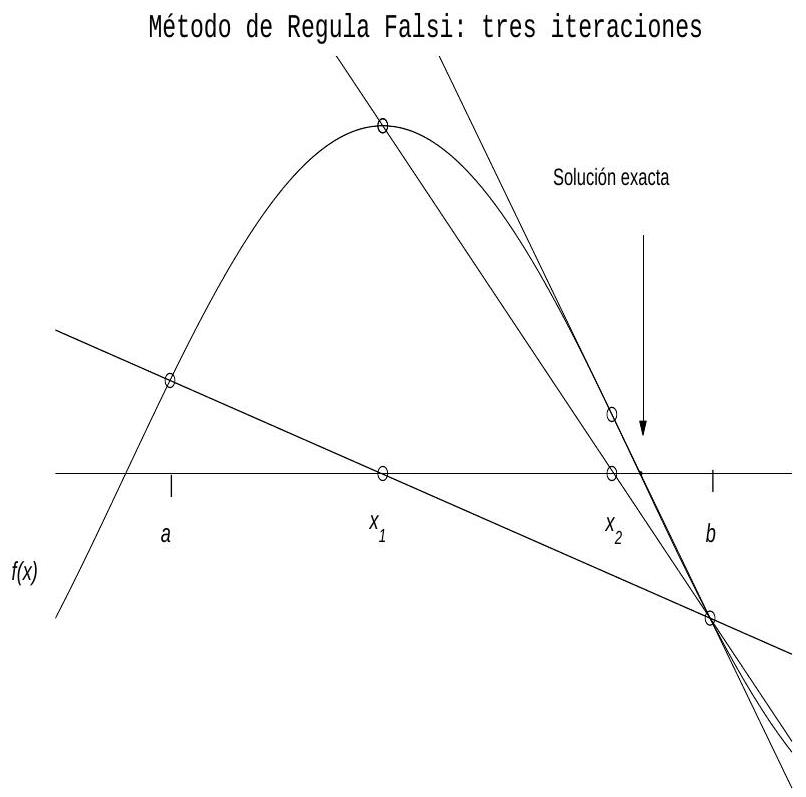
\includegraphics[width=\textwidth]{2025_09_05_3888c9ac96bd653d96b4g-073}
\captionsetup{labelformat=empty}
\caption{Figura 4.1.}
\end{center}
\end{figure}

\section{Método de Newton-Raphson}
La idea del método es "ir por la tangente" como se describe a continuación.\\
Se empieza con $x_{0}$. Se traza la tangente en $x_{0}$ y se define $x_{1}$ como la intersección de la tangente con el eje $x$. Luego se traza la tangente por $x_{1}$ y se toma $x_{2}$ la intersección de la tangente con el eje $x$, y así sucesivamente. Esto genera una sucesión $x_{n}$ como muestra la Figura 4.2.

Observemos que hace falta que $f$ sea derivable. Además, puede ocurrir que la sucesión que produce este método no sea convergente. Esto último se puede ver gráficamente con el ejemplo que muestra la Figura 4.3.

Sin embargo veremos que el método converge muy rápidamente si $x_{0}$ está "suficientemente cerca" de una raíz, bajo condiciones bastante generales sobre la función $f$.

\section*{Descripción analítica de método de Newton-Raphson.}
Sea $f:[a, b] \rightarrow \mathbb{R}$ derivable, $x_{0} \in[a, b]$, se toma $x_{1}$ tal que

$$
f\left(x_{0}\right)+\left(x_{1}-x_{0}\right) f^{\prime}\left(x_{0}\right)=0
$$

Y en general, se toma $x_{n+1}$ tal que

$$
f\left(x_{n}\right)+\left(x_{n+1}-x_{n}\right) f^{\prime}\left(x_{n}\right)=0
$$

\begin{figure}[h]
\begin{center}
  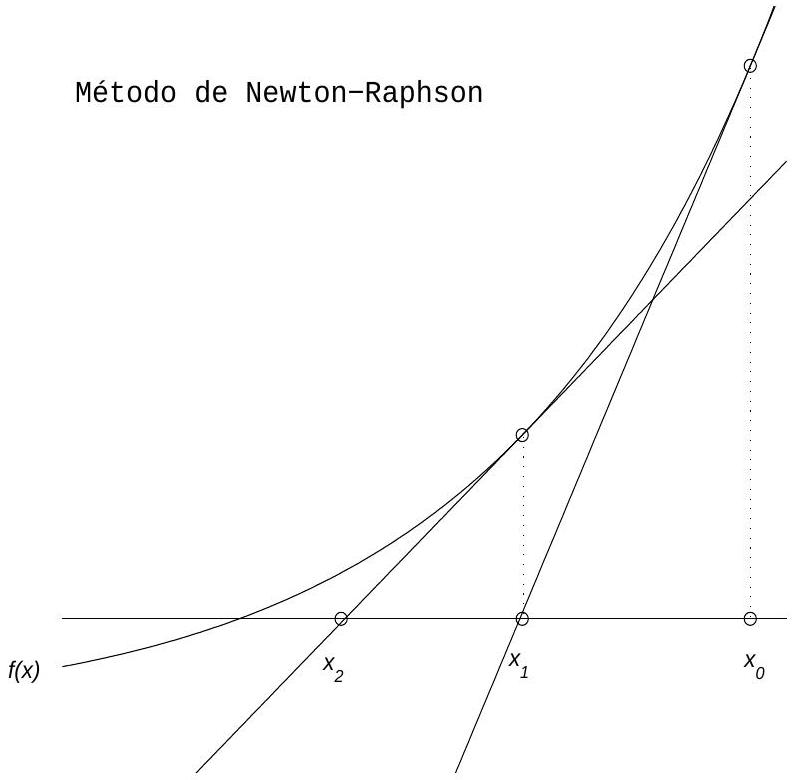
\includegraphics[width=\textwidth]{2025_09_05_3888c9ac96bd653d96b4g-074(1)}
\captionsetup{labelformat=empty}
\caption{Figura 4.2.}
\end{center}
\end{figure}

\begin{figure}[h]
\begin{center}
  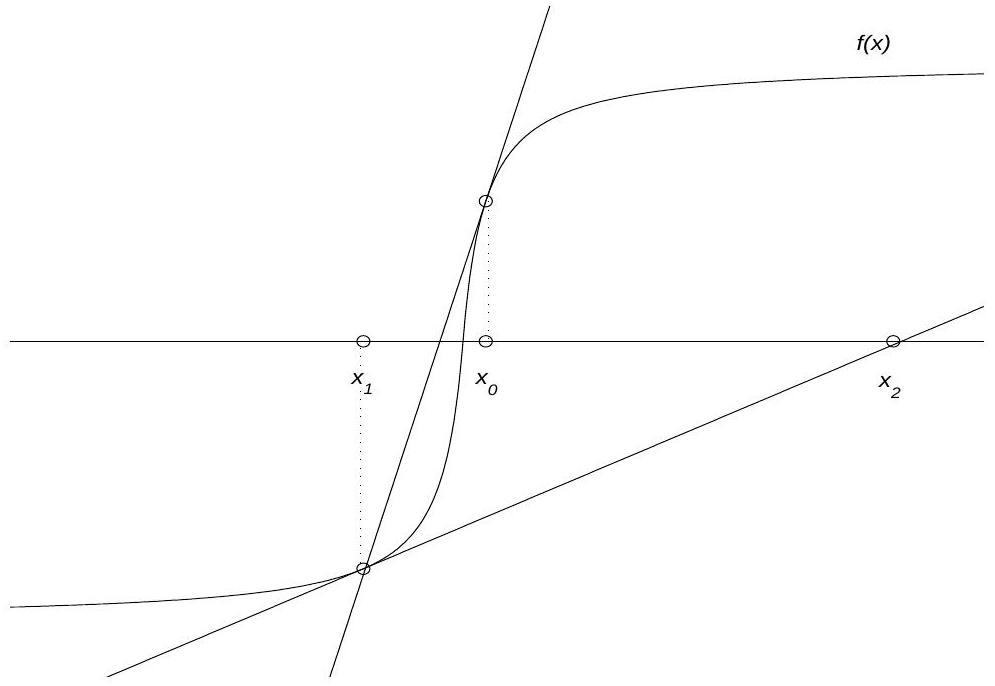
\includegraphics[width=\textwidth]{2025_09_05_3888c9ac96bd653d96b4g-074}
\captionsetup{labelformat=empty}
\caption{Figura 4.3.}
\end{center}
\end{figure}

o sea,

$$
x_{n+1}=x_{n}-\frac{f\left(x_{n}\right)}{f^{\prime}\left(x_{n}\right)}
$$

Observemos que para que esto tenga sentido, hay que suponer $f^{\prime}\left(x_{n}\right) \neq 0$, esto es obvio gráficamente como muestra la figura 4.3.

Observación 4.4. Si $f^{\prime}$ es continua, una sucesión $\left(x_{n}\right)$ construida con este método, si converge, converge a una raíz de $f$.

Demostración. Se $r=\operatorname{lím} x_{n}$. Tenemos

$$
f^{\prime}\left(x_{n}\right)\left(x_{n+1}-x_{n}\right)=f\left(x_{n}\right) .
$$

Como $f$ y $f^{\prime}$ son continuas, al tomar límite queda $0=f^{\prime}(r)(r-r)=f(r)$.

Notemos que, En efecto,\\
Ahora analicemos la convergencia del método. Sea $r$ una raíz simple de $f$, es decir, $f(r)=0$, $f^{\prime}(r) \neq 0$ y supongamos que $f^{\prime \prime}$ es acotada.

Debemos estimar el error que se comete al usar $x_{n}$ en lugar de la solución exacta (y desconocida) $r$. Esto es, estudiamos la expresión $e_{n}=x_{n}-r$ y vemos si $e_{n} \rightarrow 0$.

\begin{figure}[h]
\begin{center}
  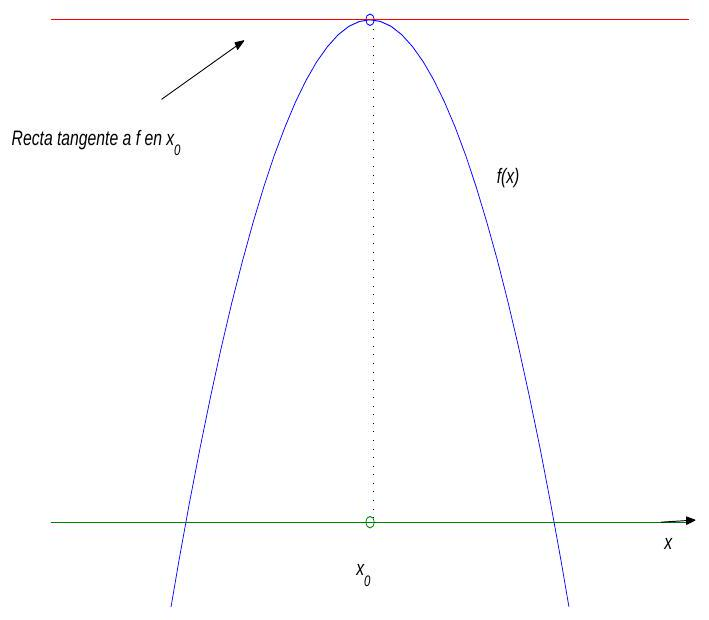
\includegraphics[width=\textwidth]{2025_09_05_3888c9ac96bd653d96b4g-075}
\captionsetup{labelformat=empty}
\caption{Figura 4.4.}
\end{center}
\end{figure}

Para analizar la convergencia del error miramos la sucesión recursiva

$$
e_{n+1}=x_{n+1}-r=x_{n}-\frac{f\left(x_{n}\right)}{f^{\prime}\left(x_{n}\right)}-r=e_{n}-\frac{f\left(x_{n}\right)}{f^{\prime}\left(x_{n}\right)}
$$

entonces


\begin{equation*}
e_{n+1}=\frac{e_{n} f^{\prime}\left(x_{n}\right)-f\left(x_{n}\right)}{f^{\prime}\left(x_{n}\right)} \tag{4.1}
\end{equation*}


Observemos que si $f^{\prime}(r) \neq 0$ entonces $f^{\prime}\left(x_{n}\right) \neq 0$ para $x_{n}$ cercano a $r$ (esto lo justificaremos con más precisión después).

Usando el desarrollo de Taylor de orden 2 centrado en la raíz $r$ se tiene,

$$
0=f(r)=f\left(x_{n}\right)-\left(x_{n}-r\right) f^{\prime}\left(x_{n}\right)+\frac{1}{2}\left(x_{n}-r\right)^{2} f^{\prime \prime}(\xi)
$$

donde $\xi$ es un valor intermedio entre $x_{n}$ y $r$. Entonces

$$
e_{n} f^{\prime}\left(x_{n}\right)-f\left(x_{n}\right)=\frac{1}{2} f^{\prime \prime}(\xi) e_{n}^{2}
$$

Reemplazando en la igualdad 4.1 queda


\begin{equation*}
e_{n+1}=\frac{1}{2} \frac{f^{\prime \prime}(\xi)}{f^{\prime}\left(x_{n}\right)} e_{n}^{2} \tag{4.2}
\end{equation*}


Con todo esto podemos demostrar el siguiente teorema.\\
TEOREMA 4.5. (de convergencia) Si $r$ es un cero simple de $f\left(\right.$ i.e. $f^{\prime}(r) \neq 0$ ) y sea $I= [r-\alpha, r+\alpha]$ un intervalo tal que $\left|f^{\prime}(x)\right| \geq \delta>0 y\left|f^{\prime \prime}(x)\right| \leq M$ en I. Entonces,

Existe $\varepsilon>0$ tal que $I_{\varepsilon}=[r-\varepsilon, r+\varepsilon] \subset I$ y se tiene que $\left|e_{n}\right| \rightarrow 0 y$


\begin{equation*}
\left|e_{n+1}\right| \leq \frac{1}{2} \frac{M}{\delta}\left|e_{n}\right|^{2}, \tag{4.3}
\end{equation*}


siempre que $x_{0} \in I_{\varepsilon}$.

Demostración. Como las cotas para $f^{\prime}$ y $f^{\prime \prime}$ siguen siendo ciertas para cualquier subintervalo de $I$, podemos elegir $\varepsilon>0$ tal que

$$
\frac{1}{2} \frac{M}{\delta} \varepsilon=\lambda<1 .
$$

Entonces, si $x_{0} \in I_{\varepsilon}$ tenemos que $\left|e_{0}\right|=\left|x_{0}-r\right|<\varepsilon$ y usando (4.2) obtenemos

$$
\left|e_{1}\right|=\left|x_{1}-r\right| \leq \lambda\left|e_{0}\right| .
$$

En particular, $x_{1} \in I_{\varepsilon}$. Análogamente,

$$
\left|e_{2}\right|=\left|x_{2}-r\right| \leq \lambda\left|e_{1}\right| \leq \lambda^{2}\left|e_{0}\right|
$$

y $x_{2} \in I_{\varepsilon}$. Continuando de esta manera, obtenemos una sucesión $\left(x_{n}\right)_{n \in \mathbb{N}} \subset I_{\varepsilon}$ tal que

$$
\left|e_{n}\right| \leq \lambda^{n}\left|e_{0}\right| .
$$

Como $0<\lambda<1$ se tiene que $\left|e_{n}\right| \rightarrow 0$ si $n \rightarrow \infty$. Finalmente, la desigualdad (4.3) se obtiene de (4.2).

Corolario 4.6. Si $f^{\prime}$ es continua y $f^{\prime \prime}$ es acotada en $[a, b]$ y $r \in[a, b]$ es una raíz simple de $f$, entonces existe un $\varepsilon>0$ tal que si $x_{0} \in I_{\varepsilon}=[r-\varepsilon, r+\varepsilon] \subset[a, b]$, el método de Newton empezando en $x_{0}$ converge a $r$.

Demostración. Como $f^{\prime}(r) \neq 0$ y $f^{\prime}$ es continua, existen $\alpha>0$ y $\delta>0$ tales que $I=[r-\alpha, r+\alpha] \subset [a, b]$ y $\left|f^{\prime}(x)\right|>\delta$ para todo $x \in I$. Ahora estamos en las condiciones del teorema 4.5.

Observación 4.7. Un caso particular del corolario 4.6 es una función $C^{2}([a, b])$ que tiene a $r \in[a, b]$ como raíz simple.

Ahora, queremos estudiar la rápidez con la que una sucesión generada por un método, converge a la solución exacta. Para eso necesitamos la siguiente

Definición 4.8. En general podemos definir que un método es de orden $p$ si existe una constante $C>0$ tal que

$$
\lim _{n \rightarrow \infty} \frac{\left|e_{n+1}\right|}{\left|e_{n}\right|^{p}}=C \quad y \quad \lim _{n \rightarrow \infty} \frac{\left|e_{n+1}\right|}{\left|e_{n}\right|^{p-\varepsilon}}=0
$$

Observemos primero que cuanto más grande sea $p$ mejor. Ahora, veamos qué significa esto geométricamente. Para valores grandes de $n$, es decir, asintóticamente, se puede considerar que el comportamiento de las sucesiones $\left|e_{n+1}\right|$ y $\left|e_{n}\right|^{p}$ son equivalentes, lo que se expresa como

$$
\left|e_{n+1}\right| \sim C\left|e_{n}\right|^{p}
$$

Por otra parte, si se obtiene una desigualdad de la forma

$$
\left|e_{n+1}\right| \leq C\left|e_{n}\right|^{p}
$$

podemos asegurar que el orden de convergencia es por lo menos $p$.

La convergencia para el método de Newton-Raphson es cuadrática, es decir, $p=2$. Si bien, con la desigualdad (4.3) podemos asegurar que existe $C>0$ tal que

$$
\left|e_{n+1}\right| \leq C\left|e_{n}\right|^{2}
$$

de la igualdad (4.2) se deduce que el método, en general, converge cuadráticamente. Esto es, en cada paso el error se reduce cuadráticamente (o sea es menor o igual que el cuadrado del error del paso anterior).

Esta es la gran ventaja del método de Newton. El número de cifras correctas se duplica (esencialmente) en un paso.

Este resultado de convergencia es "local", o sea, el teorema garantiza la convergencia si se empieza "suficientemente cerca" de $r$. En la práctica es un tema difícil determinar lo que es "suficientemente cerca". Muchas veces, se combinan unos pasos del método de bisección para encontrar un intervalo en el que se aplique el Teorema 4.5. Sin embargo, el método de Newton funciona en forma excelente (incluso en $N$ variables) y es de los más usados.

Ejemplo 4.9. Calculemos, aplicando el método de Newton una aproximación de $\sqrt{2}$. Comparemos el resultado con el que se obtuvo al aplicar el método de bisección. Como antes la función es $f(x)=x^{2}-2$ y elegimos $x_{0}=3$. Tenemos


\begin{equation*}
x_{n+1}=x_{n}-\frac{f\left(x_{n}\right)}{f^{\prime}\left(x_{n}\right)}=x_{n}-\frac{x_{n}^{2}-2}{2 x_{n}}=\frac{x_{n}}{2}+\frac{1}{x_{n}} \tag{4.4}
\end{equation*}


Y aplicando esto obtenemos

$$
\begin{array}{ll}
x_{0}=3 & x_{3}=1,41499843 \ldots \\
x_{1}=1,833 \ldots & x_{4}=1,41421378 \ldots \\
x_{2}=1,4621212 \ldots & x_{5}=1,414213562 \ldots
\end{array}
$$

Observemos que

$$
\sqrt{2}=1,414213562 \ldots
$$

Es decir, con cinco pasos del método tenemos más de diez cifras exactas, mientras que con bisección en ocho pasos teníamos cuatro cifras exactas.

Comentario. Hacia el año 2000 a.C. los Babilonios usaban el siguiente método para "calcular" el número $\sqrt{p}$ si $p \in \mathbb{N}$. Si $a>\sqrt{p}$ se tiene que $\frac{p}{a}<\sqrt{p}$. Luego $\sqrt{p}$ es un número entre $\frac{p}{a}$ y $a$. Entonces, consideraban el promedio $\frac{1}{2}\left(a+\frac{p}{a}\right)$ como primera aproximación, así sucesivamente. Esto coincide con el método de Newton, de 1669 d.C., aplicado a la función $x^{2}-p$. Comparar con (4.4).\\
Ejemplo 4.10. Como segundo ejemplo veamos qué sucede con $f(x)=x^{3}, r=0$. Es claro que la única raíz es $r=0$. Lo que se pretende con este ejemplo es mostrar alguna de las dificultades\\
a tener en cuenta cuando se aplica el método de Newton. La sucesión que produce este método es:

$$
x_{n+1}=x_{n}-\frac{x_{n}^{3}}{3 x_{n}^{2}}=\frac{2}{3} x_{n}
$$

Entonces

$$
\left|e_{n+1}\right|=\frac{2}{3}\left|e_{n}\right|
$$

En este caso, observamos que la convergencia es lineal y no es cuadrática. Lo que sucede es que no se verifica la hipótesis de que $r$ sea una raíz simple ( $f^{\prime}(r)=0$ en este caso).\\
Ejemplo 4.11. Este es un ejemplo donde el método de Newton-Raphson no converge. En este caso, la hipótesis que no se cumple es la derivabilidad de $f$. Consideremos la función

$$
f(x)= \begin{cases}\sqrt{x} & x \geq 0 \\ -\sqrt{-x} & x<0\end{cases}
$$

$\operatorname{con} r=0$.\\
Un cálculo sencillo permite ver que $f$ no es derivable en la raíz. En cualquier otro valor se tiene

$$
f^{\prime}(x)= \begin{cases}\frac{1}{2} x^{-\frac{1}{2}} & x>0 \\ \frac{1}{2}(-x)^{-\frac{1}{2}} & x<0\end{cases}
$$

Es decir,

$$
f^{\prime}(x)=\frac{1}{2}|x|^{-\frac{1}{2}}
$$

La sueción que produce el método se escribe como

$$
x_{n+1}=x_{n}-\frac{x_{n}^{\frac{1}{2}}}{\frac{1}{2} x_{n}^{-\frac{1}{2}}}=x_{n}-2 x_{n}=-x_{n}
$$

Ahora, salvo que comencemos en la raíz (con lo cual no necesitaríamos de un método para hallarla) se tiene que $x_{n}$ es positivo o negativo.

Supongamos que $x_{n}>0$, entonces $x_{n+1}=-x_{n}<0$ y $x_{n+2}=-x_{n+1}>0$.\\
Si seguimos el proceso que genera $x_{n}$ desde un $x_{0}$ inicial vemos que la sucesión es:

$$
x_{0} \quad \rightarrow \quad-x_{0} \quad \rightarrow \quad x_{0} \quad \rightarrow \quad-x_{0} \quad \rightarrow \ldots
$$

Concluimos que, en este ejemplo, el método de Newton no converge para ningún $x_{0}$ por más cerca de $r=0$ que esté.

Ahora veamos un teorema de convergencia global para el método de Newton que se aplica a funciones convexas. Una función se dice convexa en $(a, b)$ si la recta tangente al gráfico de $f$ está por debajo de éste para todo los $x$ en el intervalo. Si la función es dos veces derivable esto corresponde con la condición $f^{\prime \prime} \geq 0$.

Teorema 4.12. Sea $f$ dos veces derivable en $\mathbb{R}$ tal que $f^{\prime \prime}>0$ y $f$ cambia de signo. Dado cualquier valor inicial $x_{0}$, si $f$ no alcanza su mínimo en $x_{0}$ entonces, el método de NewtonRaphson.

Demostración. Supongamos que $f$ es monótona creciente. En este caso, $f$ tiene una única raíz, $r$.

Si $x_{0}>r$ entonces $x_{1}<x_{0}$ pues $x_{1}=x_{0}-\frac{f\left(x_{0}\right)}{f^{\prime}\left(x_{0}\right)}$ con $f\left(x_{0}\right)$ y $f^{\prime}\left(x_{0}\right)$ positivos. Ahora, usando el desarrollo de orden 2 de Taylor en $x_{0}$ evaluado en $r$, queda que $0=f(r) \geq f\left(x_{0}\right)+f^{\prime}\left(x_{0}\right)\left(r-x_{0}\right)$. Además, la definición de $x_{1}$ queda $f\left(x_{0}\right)+f^{\prime}\left(x_{0}\right)\left(x_{1}-x_{0}\right)=0$. Así,


\begin{equation*}
f\left(x_{0}\right)+f^{\prime}\left(x_{0}\right)\left(x_{1}-x_{0}\right) \geq f\left(x_{0}\right)+f^{\prime}\left(x_{0}\right)\left(r-x_{0}\right) . \tag{4.5}
\end{equation*}


Y, por lo tanto, $x_{1}>r$. Si se llega en finitos pasos a la raíz, el método es convergente. Si no, con el razonamiento de arriba podemos ver que el método genera una sucesión $x_{n}$ monótona y acotada:

$$
x_{0}>x_{1}>x_{2}>\ldots>x_{n}>\ldots>r .
$$

Luego, es convergente. Por la Observación 4.4, $\left(x_{n}\right)$ converge a una raíz de $f$. Como supusimos $f$ monótona, la raíz es $r$.

Si $f$ es monótona decreciente, una demostración análoga prueba el resultado. Finalmente, si $f$ no es monótona, $f$ tiene un mínimo que lo alcanza en algún valor, digamos $x^{*}$. Por hipótesis, tomamos un valos inicial $x_{0} \neq x^{*}$. Supongamos que $x_{0}>x^{*}$, el caso $x_{0}<x^{*}$ es análogo. Si $x_{0}>r$ se repiten los pasos del caso $f$ monótona creciente. Si por el contrario $x_{0}<r$, de (4.5), se sigue que $x_{1}>r$ y procedemos tomando $x_{1}$ como valor inicial.

Si bien este teorema es bastante claro geométricamente para funciones definidas en $\mathbb{R}$, su interés radica en su extensión a $\mathbb{R}^{N}$.

\section{Método de punto fijo}
El método de Newton puede verse como un caso particular del método de punto fijo.\\
La idea es reemplazar la ecuación $f(x)=0$ por otra de la forma $x=g(x)$ de manera que la solución de ésta sea la solución del problema original.

Esto puede hacerse de diversas maneras, por ejemplo, si

$$
f(x)=x^{3}-13 x+18
$$

podemos tomar $g(x)$ como cualquiera de las siguientes funciones

$$
g_{1}(x)=\frac{x^{3}+18}{13}, \quad g_{2}(x)=(13 x-18)^{\frac{1}{3}}, \quad g_{3}(x)=\frac{13 x-18}{x^{2}}
$$

Una vez encontrada $g$ una función continua, el problema se reduje a encontrar puntos fijos de $g$, es decir, $r$ tales que

$$
r=g(r)
$$

Se define una sucesión por iteración, se elige un $x_{0}$ y después se toma


\begin{equation*}
x_{n+1}=g\left(x_{n}\right) \tag{4.6}
\end{equation*}


Observemos que si la sucesión generada por (4.6) $x_{n}$ converge, entonces lo hace a un punto fijo de $g$. En efecto, tomando límite y usando que $g$ es continua se tiene que si $x_{n} \rightarrow r$ entonces $r=g(r)$.

Teorema 4.13. Sea $I=[a, b]$ si $g(I) \subset I$ entonces $g$ tiene al menos un punto fijo en $I$.

Demostración. Como $g(I) \subset I$ se tiene que $a \leq g(a) \leq b$ y $a \leq g(b) \leq b$, si $a=g(a)$ o $b=g(b)$ listo. Si no, $g(a)-a>0$ y $g(b)-b<0$. Entonces la función $F(x)=g(x)-x$ cumple, $F(a)>0$ y $F(b)<0$ y como $F$ es continua existe un $r$ en $I$ tal que $0=F(r)=g(r)-r$.

Teorema 4.14. Si $g$ es además derivable $y\left|g^{\prime}(x)\right| \leq \lambda<1 \forall x \in I$ y $g(I) \subset I$ entonces $g$ tiene un único punto fijo.

Demostración. Si hay dos puntos fijos, $r_{1}, r_{2}$ con $r_{1} \neq r_{2}$, tenemos

$$
\left|r_{1}-r_{2}\right|=\left|g\left(r_{1}\right)-g\left(r_{2}\right)\right|=\left|g^{\prime}(\xi)\left(r_{1}-r_{2}\right)\right| \leq \lambda\left|r_{1}-r_{2}\right|<\left|r_{1}-r_{2}\right|
$$

una contradicción.

Bajo estas mismas hipótesis, la sucesión generada iterativamente converge y se puede dar una cota del error en términos de $\lambda$.

Teorema 4.15. Sea $g$ tal que $\left|g^{\prime}(x)\right| \leq \lambda<1 \forall x \in I$ y $g(I) \subset I$ entonces la sucesión $x_{n}$ definida por

$$
x_{n+1}=g\left(x_{n}\right)
$$

converge al único punto fijo de $g$ y además,

\begin{enumerate}
  \item $\left|x_{n}-r\right| \leq \lambda^{n}\left|x_{0}-r\right|$
  \item $\left|e_{n}\right| \leq \frac{\lambda^{n}}{1-\lambda}\left|x_{1}-x_{0}\right|$. O sea, se tiene una acotación en términos de $\left|x_{1}-x_{0}\right|$ que es conocido.
\end{enumerate}

Demostración. Por el teorema anterior sabemos que existe un único punto fijo de $g$ que llamamos $r$. La hipótesis sobre la derivada de $g$ implica que $|g(x)-g(y)| \leq \lambda|x-y|$, o sea $g$ es Lipschitz con constante $\lambda$. Entonces

$$
\left|x_{n+1}-r\right|=\left|g\left(x_{n}\right)-g(r)\right| \leq \lambda\left|x_{n}-r\right|
$$

y de aquí, como $\lambda<1$ se tiene que

$$
\left|x_{n}-r\right| \leq \lambda^{n}\left|x_{0}-r\right| \rightarrow 0 .
$$

En particular demostramos que $x_{n} \rightarrow r$.\\
Por otra parte, intercalando $x_{1}$ y usando desigualdad triangular,

$$
\left|x_{0}-r\right| \leq\left|x_{0}-x_{1}\right|+\left|x_{1}-r\right| \leq\left|x_{0}-x_{1}\right|+\lambda\left|x_{0}-r\right| .
$$

Entonces

$$
(1-\lambda)\left|x_{0}-r\right| \leq\left|x_{1}-x_{0}\right|
$$

y como

$$
\left|x_{n}-r\right| \leq \lambda^{n}\left|x_{0}-r\right|
$$

se obtine la estimación 2).

La figura 4.5 muestra gráficamente como se genera una sucesión por el método de punto fijo. En dicho gráfico $0<f^{\prime}(x)<1$.

Para aplicar el teorema 4.15 hay que garantizar que $g(I) \subset I$ (o sea primero hay que encontrar un tal $I$ ).

Si $r$ es un punto fijo de $g$ con $\left|g^{\prime}(r)\right|<1$ este intervalo $I$ existe, resultado que probamos en el siguiente teorema.

Teorema 4.16. $g^{\prime}$ continua en $(a, b), r \in(a, b)$ un punto fijo de $g$. Si $\left|g^{\prime}(r)\right|<1$, entonces existe $\varepsilon>0$ tal que la iteración es convergente siempre que $x_{0} \in I_{\varepsilon}=(r-\varepsilon, r+\varepsilon)$.

\begin{figure}[h]
\begin{center}
  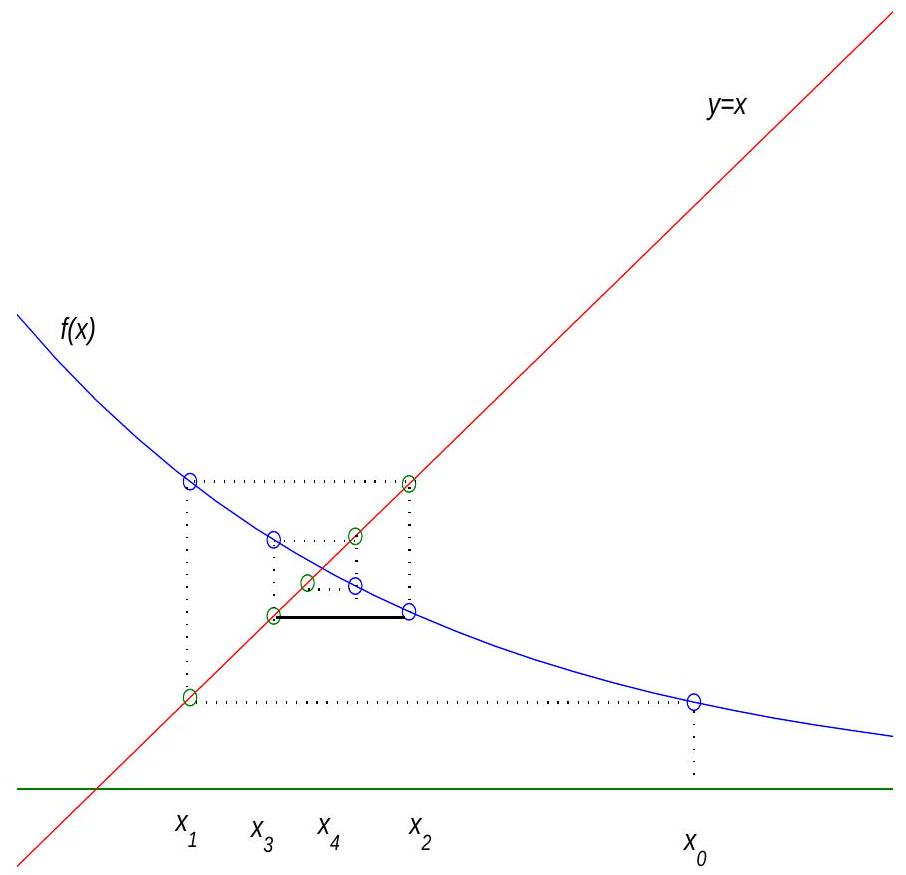
\includegraphics[width=\textwidth]{2025_09_05_3888c9ac96bd653d96b4g-083}
\captionsetup{labelformat=empty}
\caption{Figura 4.5.}
\end{center}
\end{figure}

Demostración. Como $\left|g^{\prime}(r)\right|<1$, existe una constante $K<1$ y un $\varepsilon>0$ tales que $\left|g^{\prime}(x)\right|<K$, $\forall x \in I_{\varepsilon}=(r-\varepsilon, r+\varepsilon)$ (por la continuidad de $g^{\prime}$ ). Entonces, $\forall x \in I_{\varepsilon}$,

$$
|g(x)-r|=|g(x)-g(r)| \leq K|x-r| \leq K \varepsilon<\varepsilon
$$

o sea, $g\left(I_{\varepsilon}\right) \subset I_{\varepsilon}$, y podemos aplicar el teorema anterior en $I_{\varepsilon}$.

\section{Método de la secante}
En este método tenemos que $x_{n+1}$ es función de $x_{n}$ y de $x_{n-1}$. La idea es la misma que en el método "regula falsi", trazar la secante, pero este método es diferente pues se usan las dos últimas aproximaciones $x_{n-1}$ y $x_{n}$ en lugar de encerrar la raíz como en "regula falsi". Para empezar hay que dar dos valores $x_{0}$ y $x_{1}$.

La ecuación de la secante que une los puntos $\left(x_{n-1}, f\left(x_{n-1}\right)\right)$ y $\left(x_{n}, f\left(x_{n}\right)\right)$ es

$$
y=f\left(x_{n}\right)+\left(x-x_{n}\right) \frac{f\left(x_{n}\right)-f\left(x_{n-1}\right)}{x_{n}-x_{n-1}}
$$

entonces se define $x_{n+1}$ como la intersección de esta recta con el eje $x$, así, $x_{n+1}$ verifica

$$
0=f\left(x_{n}\right)+\left(x_{n+1}-x_{n}\right) \frac{f\left(x_{n}\right)-f\left(x_{n-1}\right)}{x_{n}-x_{n-1}}
$$

es decir,

$$
x_{n+1}=x_{n}-f\left(x_{n}\right) \frac{x_{n}-x_{n-1}}{f\left(x_{n}\right)-f\left(x_{n-1}\right)} .
$$

Observemos que esta fórmula es análoga a la de Newton reemplazando $f^{\prime}$ por un cociente incremental.

La ventaja es que no hay que calcular la derivada de $f$ (esto es de gran ayuda en un caso en que $f^{\prime}$ sea difícil de calcular).

La desventaja es, según veremos, que la convergencia de la sucesión es más lenta que la que produce el método de Newton.

Observemos que la iteración del método de la secante también puede escribirse como

$$
x_{n+1}=\frac{f\left(x_{n}\right) x_{n-1}-f\left(x_{n-1}\right) x_{n}}{f\left(x_{n}\right)-f\left(x_{n-1}\right)} .
$$

Analicemos el orden de convergencia de este método, según la definición 4.8. Tenemos

$$
f(r)=0 \quad \text { y } \quad e_{n}=r-x_{n} .
$$

Luego,

$$
\begin{aligned}
e_{n+1}=r-x_{n+1} & =r-\frac{f\left(x_{n}\right) x_{n-1}-f\left(x_{n-1}\right) x_{n}}{f\left(x_{n}\right)-f\left(x_{n-1}\right)} \\
& =\frac{e_{n-1} f\left(x_{n}\right)-e_{n} f\left(x_{n-1}\right)}{f\left(x_{n}\right)-f\left(x_{n-1}\right)} \\
& =\frac{e_{n-1}\left(f\left(x_{n}\right)-f(r)\right)-e_{n}\left(f(r)-f\left(x_{n-1}\right)\right)}{f\left(x_{n}\right)-f\left(x_{n-1}\right)} \\
& =\frac{-e_{n} e_{n-1} \frac{f\left(x_{n}\right)-f(r)}{x_{n}-r}+e_{n} e_{n-1} \frac{f(r)-f\left(x_{n-1}\right)}{x_{n-1}-r}}{f\left(x_{n}\right)-f\left(x_{n-1}\right)} .
\end{aligned}
$$

Es decir,


\begin{equation*}
e_{n+1}=e_{n} e_{n-1} \frac{\frac{f\left(x_{n-1}\right)-f(r)}{x_{n-1}-r}-\frac{f(r)-f\left(x_{n}\right)}{x_{n}-r}}{f\left(x_{n}\right)-f\left(x_{n-1}\right)} . \tag{4.7}
\end{equation*}


Definamos ahora las diferencias.\\
Primera diferencia :

$$
f[a, b]=\frac{f(b)-f(a)}{b-a}=f^{\prime}(\xi)
$$

Segunda diferencia :

$$
f[a, b, c]=\frac{\frac{f(c)-f(b)}{c-b}-\frac{f(b)-f(a)}{b-a}}{c-a}
$$

Entonces el error del método de la secante verifica,

$$
e_{n+1}=-e_{n} e_{n-1} \frac{f\left[x_{n-1}, r, x_{n}\right]}{f\left[x_{n-1}, x_{n}\right]}
$$

Lema 4.17.

$$
f[a, b, c]=\frac{1}{2} f^{\prime \prime}(\eta)
$$

Demostración.

$$
f(x)=f(a)+f[a, b](x-a)+f[a, b, c](x-a)(x-b)+\text { Resto. }
$$

Despreciamos el resto y nos quedamos con el polinomio de grado 2 :

$$
f(a)+f[a, b](x-a)+f[a, b, c](x-a)(x-b)
$$

Se verá más adelante que este polinomio es el polinomio interpolador de grado dos.\\
Sea


\begin{equation*}
g(x)=f(x)-f(a)+f[a, b](x-a)+f[a, b, c](x-a)(x-b) \tag{4.8}
\end{equation*}


$g$ cumple que $g(a)=0, g(b)=0$ y $g(c)=0$.\\
Entonces $g^{\prime}$ se anula en por lo menos dos puntos y de ahí que existe $\eta$ con $g^{\prime \prime}(\eta)=0$. Ahora, derivando dos veces la expresión (4.8) y evaluando en $\eta$ se obtiene

$$
0=g^{\prime \prime}(\eta)=f^{\prime \prime}(\eta)-2 f[a, b, c]
$$

es decir,

$$
f[a, b, c]=\frac{1}{2} f^{\prime \prime}(\eta) .
$$

Aplicando el lema 4.17 a nuestra expresión de $e_{n+1}$ dada en (4.7) queda

$$
e_{n+1}=-\frac{1}{2} \frac{f^{\prime \prime}\left(\eta_{n}\right)}{f^{\prime}\left(\xi_{n}\right)} e_{n} e_{n-1}
$$

y de acá se puede deducir la convergencia local.\\
Teorema 4.18. Si $f^{\prime}(r) \neq 0,\left|f^{\prime \prime}\right| \leq K$ en un entorno de $r$ y $x_{0}, x_{1}$ están suficientemente cerca de $r$, es decir existe $\varepsilon>0$ tal que si $x_{0}, x_{1} \in I_{\varepsilon}=(r-\varepsilon, r+\varepsilon)$, entonces

$$
e_{n} \rightarrow 0 .
$$

Demostración. Existe $\varepsilon>0$ tal que $\left|f^{\prime}\right|>\delta$ en $I_{\varepsilon}$, entonces si $x_{0}, x_{1} \in I_{\varepsilon}$ tenemos que

$$
\left|e_{2}\right| \leq \frac{K}{2 \delta}\left|e_{1}\right|\left|e_{0}\right| \leq \frac{K}{2 \delta} \varepsilon^{2}
$$

y si ahora pedimos (quizás achicando el $\varepsilon$ ) que

$$
\frac{K}{2 \delta} \varepsilon=\lambda<1
$$

nos queda que

$$
\left|e_{2}\right| \leq \lambda \varepsilon<\varepsilon
$$

y entonces $x_{2} \in I_{\varepsilon}$. Ahora bien

$$
\begin{gathered}
\left|e_{3}\right| \leq \frac{K}{2 \delta}\left|e_{2}\right|\left|e_{1}\right| \leq \frac{K}{2 \delta} \lambda \varepsilon^{2} \leq \lambda^{2} \varepsilon \\
\left|e_{4}\right| \leq \frac{K}{2 \delta}\left|e_{3}\right|\left|e_{2}\right| \leq \frac{K}{2 \delta} \varepsilon \lambda^{2} \varepsilon \lambda \leq \lambda^{3} \varepsilon .
\end{gathered}
$$

Y podemos concluir por inducción que

$$
\left|e_{n}\right| \leq \lambda^{n-1} \varepsilon \rightarrow 0 .
$$

Veamos el orden de convergencia del método de la secante, teníamos

$$
\left|e_{n+1}\right|=\left|-\frac{1}{2} \frac{f^{\prime \prime}\left(\eta_{n}\right)}{f^{\prime}\left(\xi_{n}\right)}\right|\left|e_{n}\right|\left|e_{n-1}\right|=c_{n}\left|e_{n}\right|\left|e_{n-1}\right|
$$

y además, si llamamos $c_{\infty}$ al límite de $c_{n}$ tenemos

$$
c_{n} \rightarrow c_{\infty}=\left|\frac{1}{2} \frac{f^{\prime \prime}(r)}{f^{\prime}(r)}\right|
$$

Supongamos que $f^{\prime \prime}(r) \neq 0$, de esta forma $c_{\infty} \neq 0$.

Buscamos $p$ tal que

$$
\lim _{n \rightarrow \infty} \frac{\left|e_{n+1}\right|}{\left|e_{n}\right|^{p}}=C \neq 0
$$

Tenemos

$$
\frac{\left|e_{n+1}\right|}{\left|e_{n}\right|^{p}}=c_{n}\left|e_{n}\right|^{1-p}\left|e_{n-1}\right|=c_{n}\left(\frac{\left|e_{n}\right|}{\left|e_{n-1}\right|^{p}}\right)^{\alpha}
$$

Si $\alpha=1-p$ y $\alpha p=-1$, o sea

$$
p-p^{2}=\alpha p=-1
$$

entonces $p$ es solución de

$$
p^{2}-p-1=0
$$

y como $p>0$,

$$
p=\frac{1+\sqrt{5}}{2}=1,618 \ldots
$$

Con esta elección de $p$ tenemos que

$$
y_{n}=\frac{\left|e_{n+1}\right|}{\left|e_{n}\right|^{p}}
$$

cumple la iteración de punto fijo (salvo que $c_{n}$ es variable pero converge a $c_{\infty}$ ),

$$
y_{n+1}=c_{n} y_{n}^{-\frac{1}{p}}
$$

Entonces, $y_{n}$ converge al punto fijo de la ecuación $x=c_{\infty} x^{-\frac{1}{p}}$ (esto es cierto porque $p>1$ y se ve directamente escribiendo la iteración). El punto fijo es $\bar{x}=c_{\infty}^{\frac{1}{p}}$. Entonces nos queda que

$$
\frac{\left|e_{n+1}\right|}{\left|e_{n}\right|^{p}} \sim\left|\frac{1}{2} \frac{f^{\prime \prime}(r)}{f^{\prime}(r)}\right|^{\frac{1}{p}},
$$

para $n$ grande.

Ahora veamos una idea intuitiva de la demostración directamente.\\
Si suponemos $\left|e_{n+1}\right| \sim\left|e_{n}\right|^{p}$ tenemos $\left|e_{n+1}\right| \sim\left|e_{n}\right|^{p} \sim\left|e_{n-1}\right|^{p^{2}}$ y de la relación entre $e_{n+1}, e_{n}$ y $e_{n-1}$ se tiene $\left|e_{n-1}\right|^{p^{2}} \sim\left|e_{n-1}\right|^{p}\left|e_{n-1}\right|$. O sea, $\left|e_{n-1}\right|^{p^{2}-p-1} \sim$ cte. Luego $p>0$ tiene que ser solución de $p^{2}-p-1=0$ y entonces $p=\frac{1+\sqrt{5}}{2}=1,618 \ldots$.

\section{Ejercicios}
\begin{enumerate}
  \item Usar el método de bisección para hallar una raíz positiva de la ecuación trascendente:
\end{enumerate}

$$
2 x=\tan (x)
$$

¿Cuántos pasos hay que hacer para garantizar que el error sea menor que $10^{-5}$ ?\\
2. Hacer un programa en Matlab que ejecute los primeros 20 pasos de los métodos de bisección y Regula-Falsi para hallar una raíz de la ecuación $2 x^{3}+x-2=0$ comenzando con el intervalo $[0,1]$.\\
3. Hacer un programa en Matlab que ejecute los primeros 20 pasos de los métodos de bisección y N-R, para calcular $\sqrt[3]{2}$ comenzando con valores iniciales apropiados.\\
4. Demostrar que la ecuación

$$
f(x)=e^{x}+5 \operatorname{sen} x-2=0
$$

tiene una única raíz en el intervalo ( $0, \frac{3}{2}$ ). Encontrar las cotas necesarias de $\left|f^{\prime}\right|$ y $\left|f^{\prime \prime}\right|$ para determinar un valor inicial de modo que el método N-R converja a la raíz. Aplicar el método para hallar una aproximación de ésta. ¿Cuál es el orden de convergencia?\\
5. Considerar la función $f(x)=\frac{x}{1+|x|}$. Determinar para qué valores de $x_{0}$ la iteración N-R es convergente, para cuáles es divergente, y cuándo se obtienen ciclos periódicos.\\
6. Se quiere resolver la ecuación $f(x)=0$, donde $f(x)=e^{x}-2$. Calcular los 10 primeros términos de las sucesiones generadas por los métodos N-R y de la secante, comenzando con los valores iniciales $x_{1}=3$ para el primer método e $y_{1}=3, y_{2}=2,3$ para el segundo. Graficar simultáneamente las dos sucesiones obtenidas.\\
7. Sea $f$ una función $C^{1}$ y sea $\left(x_{n}\right)_{n \in \mathbb{N}}$ la sucesión que se obtiene de aplicar el método N-R a $f$. Supongamos que $x_{n}$ converge a $r$ y $f^{\prime}(r) \neq 0$, mostrar que $r$ es raíz de $f$.\\
8. Sea $f$ una función suave, y $a$ tal que $f(a)=0$, y $f^{\prime}(a) \neq 0$.\\
a) Suponiendo que en $(a, b], f, f^{\prime}, f^{\prime \prime}$ son positivas, probar que la iteración de N-R generada a partir de $x_{0} \in(a, b)$ converge decrecientemente hacia $a$.\\
$b)$ Con las mismas hipótesis, si $x_{1} \in\left(a, x_{0}\right)$, probar que la sucesión generada por el método de la secante a partir de $x_{0}, x_{1}$ converge decrecientemente hacia $a$.\\
9. Sea $f(x)=x^{\alpha}$. Se desea utilizar el método N-R para resolver la ecuación $f(x)=0$, comenzando con $x_{0}>0$. Analizar el comportamiento del método en los casos\\
(a) $\alpha \geq 1$\\
(b) $\alpha=\frac{1}{3}$\\
(c) $\alpha=\frac{1}{2}$\\
10. a) Sea $f(x)=\left(x-r_{1}\right)\left(x-r_{2}\right) \ldots\left(x-r_{d}\right)$ donde $r_{1}<r_{2}<\cdots<r_{d}$. Probar que si $x_{0}>r_{d}$ la sucesión de N-R converge a $r_{d}$.\\
b) Para un polinomio $P \in \mathbb{R}[x], P(x)=a_{d} x^{d}+\cdots+a_{0}, a_{d} \neq 0$, tal que sus $d$ raíces son reales y distintas, se propone el siguiente método que aproxima los valores de todas sus raíces:

\begin{enumerate}
  \item Se comienza con un valor $x_{0}$ mayor que $M=\operatorname{máx}\left\{1, \sum_{i=0}^{d-1} \frac{\left|a_{i}\right|}{\left|a_{d}\right|}\right\}$ (Dato: $M$ es una cota para el módulo de todas las raíces del polinomio).
  \item Se genera a partir de $x_{0}$ la sucesión de N-R, que, según el ítem anterior, converge a la raíz más grande de $P$, llamémosla $r_{d}$; obteniéndose de este modo un valor aproximado $\tilde{r}_{d}$.
  \item Se divide $P$ por $x-\tilde{r}_{d}$ y se desprecia el resto, dado que $r_{d} \sim \tilde{r}_{d}$. Se redefine ahora $P$ como el resultado de esta división y se comienza nuevamente desde el primer ítem, para hallar las otras raíces.\\
Aplicar este método para aproximar todas las raíces del polinomio $P(x)=2 x^{3}- 4 x+1$.
\end{enumerate}

\begin{enumerate}
  \setcounter{enumi}{10}
  \item Recordar que una raíz múltiple de un polinomio $f$ es una raíz simple del polinomio $f / \operatorname{gcd}\left(f, f^{\prime}\right)$, donde gcd indica el máximo común divisor. Hacer un programa en Matlab que aplique el método N-R a $f(x)$ y a $f(x) / \operatorname{gcd}\left(f, f^{\prime}\right)$ para hallar la raíz múltiple de
\end{enumerate}

$$
f(x)=(x-1)(x-2)^{2}
$$

Demostrar que, a pesar que la función $f$ no está en las hipótesis del método N-R, éste converge (aunque no tan velozmente como cuando la raíz múltiple se halla como solución de $\left.f / \operatorname{gcd}\left(f, f^{\prime}\right)\right)$.\\
12. Para $f$ una función $C^{2}$ que tiene una raíz de orden 2 en $x_{0}$ :\\
a) Demostrar que el método N-R converge sólo linealmente a $x_{0}$.\\
b) ¿Cuál es el orden de convergencia de la siguiente modificación?

$$
x_{n+1}=x_{n}-2 \frac{f\left(x_{n}\right)}{f^{\prime}\left(x_{n}\right)}
$$

\begin{enumerate}
  \setcounter{enumi}{12}
  \item Sea $f(x)=4 x^{3}-3 x+1=0$. La ecuación $f(x)=0$ tiene una raíz doble. Aproximarla calculando las 10 primeras iteraciones de los métodos $\mathrm{N}-\mathrm{R}$ y $\mathrm{N}-\mathrm{R}$ con la modificación del ejercicio anterior, comenzando con los valores iniciales $x_{1}=y_{1}=25$. Graficar simultáneamente las dos sucesiones obtenidas.
  \item Se quiere aplicar el método N-R para dar una tabla de valores de la función $y(x)$ definida implícitamente por la ecuación $G(x, y)=0$ en un intervalo $[a, b]$.
\end{enumerate}

El método consiste en comenzar la tabla en un par de valores $x_{0}, y_{0}$ que verifican $x_{0}=a$ y $G\left(x_{0}, y_{0}\right)=0$ y proceder por incrementos en $x$ hasta llegar al valor $x_{N}=b$.

En cada paso se obtiene el valor de $y_{n+1}$ aplicando el método N-R a la función $G\left(x_{n+1}, y\right)$ donde $y$ es la variable y $x_{n+1}$ permanece fijo; con valor inicial el valor de $y_{n}$ obtenido en el paso anterior. Dado que la función $y(x)$ se supone continua, esta elección del valor inicial se supone apropiada.\\
a) Aplicar el método para la ecuación $G(x, y)=x^{2}+y^{2}-1=0$, comenzando en $x_{0}=0, y_{0}=1$ para valores de $x$ en $[0,1]$. Graficar junto con la solución que se obtiene de despejar analíticamente y comparar. Utilizar distintos valores para el incremento y para la cantidad de iteraciones del método N-R en cada paso.\\
b) Aplicar el método para $G(x, y)=3 x^{7}+2 y^{5}-x^{3}+y^{3}-3$. Comenzar la tabla en $x_{0}=0, y_{0}=1$ y proceder por incrementos en $x$ de 0,2 hasta llegar a $x_{50}=10$.\\
15. Dada $F: \mathbb{R}^{n} \rightarrow \mathbb{R}^{n}$ el método N-R generalizado consiste en realizar la iteración vectorial

$$
x^{k+1}=x^{k}-\left(\left.D F\right|_{x^{k}}\right)^{-1} \cdot F\left(x^{k}\right),
$$

donde $\left(\left.D F\right|_{x^{k}}\right)^{-1}$ es la inversa de la matriz diferencial de $F$ evaluada en $x^{k}$.\\
Usar la versión generalizada a varias variables del método N-R para para resolver el sistema de ecuaciones

$$
2 x-3 y=0, \quad x^{2}-y^{2}-3=0
$$

comenzando con valores iniciales $\left(x_{0}, y_{0}\right)=(2,1)$.\\
16. Resolver $\cos (x)=2 x, x>0$ comenzando con $x_{0}=0,5$ y utilizando:\\
a) La iteración de punto fijo $x_{n+1}=\frac{1}{2} \cos \left(x_{n}\right)$\\
b) El método N-R.

Graficar, usando Matlab, las sucesiones obtenidas y comparar.\\
17. Sea $g$ una función tal que $g^{\prime}$ es continua en $[s, b]$, donde $s$ es un punto fijo de $g$. Si además, se verifica que $0 \leq g^{\prime}(x) \leq K<1$ para todo $x \in[s, b]$, mostrar que la iteración, comenzando con $x_{0} \in[s, b]$, converge decrecientemente a $s$.\\
18. Sea $f: \mathbb{R}_{>0} \rightarrow \mathbb{R}$ definida como $f(x)=\frac{8 x-1}{x}-e^{x}$.\\
a) Dibujar la gráfica de $f$ y determinar el número de raíces de la ecuación $f(x)=0$, localizando cada raíz entre dos enteros consecutivos.\\
b) Para cada una de las siguientes funciones:

$$
f_{1}(x)=\frac{1}{8}\left(1+x e^{x}\right), \quad f_{2}(x)=\ln \left(\frac{8 x-1}{x}\right)
$$

consideramos el siguiente método iterativo: dado $x_{0}=1$ sea

$$
x_{n+1}=f_{i}\left(x_{n}\right), n \in \mathbb{N},(i=1,2) .
$$

Estudiar si estas sucesiones convergen hacia alguna de las raíces de $f=0$.\\
c) Utilizando Matlab, estimar las raíces con estos dos métodos.\\
19. Sea $f(x)=x^{3}-x-1$. Se consideran las dos siguientes iteraciones de método de punto fijo.

$$
g(x)=x^{3}-1, \quad h(x)=\sqrt[3]{x+1}
$$

a) Determinar cuáles de estas funciones son apropiadas para la iteración.\\
b) Para las que sí lo sean:

\begin{itemize}
  \item Determinar un intervalo inicial $I$ en el cual el método converja.
  \item Dar un valor inicial $x_{0} \in I$ y la cantidad de iteraciones necesarias para aproximar la raíz de $f$ con error menor que $10^{-5}$ comenzando con el $x_{0}$ dado.
\end{itemize}

\begin{enumerate}
  \setcounter{enumi}{19}
  \item Dada la función $f(x)=x+1 / x-2, f: \mathbb{R}_{>0} \rightarrow \mathbb{R}$, se construye el siguiente algoritmo para aproximar la raíz $r=1$ :
\end{enumerate}

$$
x_{n+1}=2-1 / x_{n}
$$

a) Verificar que si $x_{0}>1$ entonces la sucesión $\left\{x_{n}\right\}$ es monótona decreciente y acotada inferiormente por 1. Concluir que $x_{n} \rightarrow 1$, aunque esta iteración no está en las hipótesis del teorema del punto fijo. ¿Qué hipótesis no se cumple?\\
b) Dar un algoritmo para aproximar la raíz de $f$ que converja cuadráticamente.\\
21. Sea $f$ una función $C^{1}$ en las condiciones del método N-R. Sea $g(x)=x-\frac{f(x)}{f^{\prime}(x)}$. Mostrar que el método N-R es un método de punto fijo.

\chapter{Interpolación}
El objetivo de este capítulo es estudiar cómo puede aproximarse una función por polinomios. Una forma de hacer esto es construir los polinomios de manera que coincidan con la función dada en algunos puntos predeterminados, lo que recibe el nombre de interpolación polinomial. Analizaremos distintos métodos para resolver este problema y estudiaremos el error que se comete al reemplazar una función por un polinomio interpolante.

Hay diversos motivos para estudiar este problema. Por un lado, el polinomio interpolante puede utilizarse para reconstruir una función $f$ a partir de una tabla de valores. Por otra parte, es una herramienta fundamental para integración y diferenciación numérica, como veremos más adelante.

\section{Interpolación de Lagrange}
En lo que sigue, si $n \in \mathbb{N}_{0}$, llamaremos $\mathcal{P}_{n}$ al conjunto de polinomios de grado menor o igual que $n$, incluyendo el polinomio nulo.

Supongamos que se sabe que la tabla de valores

\begin{center}
\begin{tabular}{|c||c|c|c|c|c|}
\hline
$\left(x_{j}\right):$ & $x_{0}$ & $x_{1}$ & $x_{2}$ & $\ldots$ & $x_{n}$ \\
\hline
$\left(y_{j}\right):$ & $y_{0}$ & $y_{1}$ & $y_{2}$ & $\ldots$ & $y_{n}$ \\
\hline
\end{tabular}
\end{center}

corresponde con datos de una función continua que se desconoce. Queremos poder modelizar dicha función por medio de un polinomio. Es decir, queremos encontrar un polinomio tal que


\begin{equation*}
p\left(x_{j}\right)=y_{j}, \quad \forall j=0,1, \ldots, n . \tag{5.1}
\end{equation*}


Nuestro primer paso será dar un resultado básico que establece que esto es posible. Mostraremos una forma concreta de hallar un polinomio $p$ que verifique (5.1) y además veremos que si el polinomio es de grado menor o igual que $n$, éste es único. Vamos a basar nuestra demostración en la Base de Lagrange que es una base de polinomios que construimos a continuación.

Base de Lagrange: Para cada punto $x_{j}, j=0, \ldots, n$, buscamos un polinomio de grado $n$ que se anule en todos los $x_{i}$ salvo $x_{j}$ donde queremos que valga 1 . Por ejemplo, $\ell_{0}$ será un polinomio en $\mathcal{P}_{n}$ tal que se anula en $x_{1}, \ldots, x_{n}$ y $\ell_{0}\left(x_{0}\right)=1$.

Como $x_{1}, \ldots, x_{n}$ son raíces de $\ell_{0}, \ell_{0}(x)=\alpha \prod_{i=1}^{n}\left(x-x_{i}\right)$; donde $\alpha$ es una constante que se elige de modo que $\ell_{0}\left(x_{0}\right)=1$. Imponiendo esta condición obtenemos

$$
\ell_{0}(x)=\frac{\prod_{i=1}^{n}\left(x-x_{i}\right)}{\prod_{i=1}^{n}\left(x_{0}-x_{i}\right)} .
$$

De manera análoga, para cada $j=1, \ldots, n$, , el polinomio $\ell_{j} \in \mathcal{P}_{n}$ tal que

$$
\ell_{j}\left(x_{i}\right)=\delta_{i j}= \begin{cases}1 & i=j \\ 0 & i \neq j\end{cases}
$$

estará dado por


\begin{equation*}
\ell_{j}(x)=\frac{\prod_{i \neq j}\left(x-x_{i}\right)}{\prod_{i \neq j}\left(x_{j}-x_{i}\right)} \tag{5.2}
\end{equation*}


Los polinomios $\left\{\ell_{0}, \ell_{1}, \ldots, \ell_{n}\right\}$ se conocen como la base de Lagrange. Vale destacar que estos polinomios sólo dependen de los datos $\left\{x_{0}, x_{1}, \ldots, x_{n}\right\}$.

TEOREMA 5.1. Dados $x_{0}, \ldots, x_{n}$ y valores $y_{0}, \ldots, y_{n}$ existe un único polinomio $p_{n} \in \mathcal{P}_{n}$ tal que

$$
p_{n}\left(x_{j}\right)=y_{j} ; \quad \forall j=0, \ldots, n .
$$

Demostración. Usando la base de Lagrange definimos


\begin{equation*}
p_{n}(x)=\sum_{j=0}^{n} y_{j} \ell_{j}(x) . \tag{5.3}
\end{equation*}


obteniendo un polinomio $p_{n} \in \mathcal{P}_{n}$ que verifica (5.1). Veamos que es único. Supongamos que hay dos polinomios $p_{n}, q_{n} \in \mathcal{P}_{n}$ que interpolan la tabla de pares ( $x_{i}, y_{i}$ ), esto es

$$
\left(p_{n}-q_{n}\right)\left(x_{j}\right)=0 \quad \forall j=0, \ldots, n .
$$

Entonces $p_{n}-q_{n}$ es un polinomio de grado menor o igual que $n$ con $n+1$ raíces distintas; es decir, $p_{n}-q_{n}$ es el polinomio nulo.

Observación 5.2. 1. La escritura (5.3) se conoce como la forma de Lagrange del polinomio interpolador.\\
2. El polinomio $p_{n}$ puede tener grado estrictamente menor que $n$. Por ejemplo, si se considera la tabla de 5 valores

\begin{center}
\begin{tabular}{|l||l|l|l|l|l|}
\hline
$\left(x_{j}\right):$ & -4 & -2 & 0 & 1 & 3 \\
\hline
$\left(y_{j}\right):$ & 9 & 5 & 1 & -1 & -5 \\
\hline
\end{tabular}
\end{center}

El polinomio de grado menor o igual que 4 que interpola la tabla es $p_{4}(x)=-2 x+1$. Gracias a la unicidad, como se trata de un polinomio de grado 1, es suficiente mostrar que en cada $x_{j}, p_{4}$ toma el valor $y_{j}$; esto es inmediato.\\
3. Si los datos corresponden con una función $f$ que es un polinomio de grado menor o igual que $n$, es decir, $f \in \mathcal{P}_{n}$ y los valores $y_{j}=f\left(x_{j}\right)$; entonces $f=p_{n}$ (la interpolación es exacta para polinomios).\\
4. El polinomio que interpola en $n+1$ puntos distintos es único en $\mathcal{P}_{n}$. Si se permite mayor grado hay infinitos. Por ejemplo, si $q$ es un polinomio cualquiera, el polinomio

$$
p(x)=(-2 x+1)+q(x)(x+4)(x+2) x(x-1)(x-3),
$$

también interpola la tabla dada arriba.

Otra forma de demostrar la existencia (y de encontrar el polinomio) es por el método de los coeficientes indeterminados. El polinomio será de la forma

$$
p_{n}(x)=a_{0}+a_{1} x+\cdots+a_{n} x^{n}
$$

y se buscan $a_{0}, \ldots, a_{n}$ tales que

$$
p_{n}\left(x_{j}\right)=y_{j}
$$

Al evaluar, queda formado un sistema $(n+1) \times(n+1)$

$$
\left(\begin{array}{ccccc}
1 & x_{0} & x_{0}^{2} & \cdots & x_{0}^{n} \\
1 & x_{1} & x_{1}^{2} & \cdots & x_{1}^{n} \\
\vdots & & & \ddots & \vdots \\
1 & x_{n} & x_{n}^{2} & \cdots & x_{n}^{n}
\end{array}\right)\left(\begin{array}{c}
a_{0} \\
a_{1} \\
\vdots \\
a_{n}
\end{array}\right)=\left(\begin{array}{c}
y_{0} \\
y_{1} \\
\vdots \\
y_{n}
\end{array}\right)
$$

La matriz de la izquierda se llama matriz de Van der Monde y como sólo depende de los datos $\left\{x_{0}, \ldots, x_{n}\right\}$ suele notarse por $V\left(x_{0}, \ldots, x_{n}\right)$.

Para ver que existe una solución $\left(a_{0}, \ldots, a_{n}\right)$ y que es única hay que ver que la matriz $V\left(x_{0}, \ldots, x_{n}\right)$ es inversible. Esto equivale a ver que el núcleo es nulo. Ahora, si $\left(a_{0}, \ldots, a_{n}\right) \in N u\left(V\left(x_{0}, \ldots, x_{n}\right)\right)$ tendríamos

$$
a_{0}+a_{1} x_{j}+a_{2} x_{j}^{2}+\ldots+a_{n} x_{j}^{n}=0 \quad \forall j=0, \ldots, n .
$$

Entonces $a_{0}=\ldots=a_{n}=0$ (pues un polinomio de grado $n$ no nulo no puede tener $n+1$ raíces distintas).

Ejemplo 5.3. Analicemos qué sucede si interpolamos la función $f(x)=x^{\frac{2}{3}}$ en el intervalo $[-1,1]$ por un polinomio considerando puntos equiespaciados.

En este caso, sin encontrar explícitamente el polinomio, si tenemos en cuenta la paridad de la función, podemos pensar que un polinomio de grado par será una buena elección. La Figura 5.1 muestra el gráfico de $f$ junto con el polinomio interpolante $p$ que se obtiene al considerar 11 puntos equiespaciados. Si consideramos la diferencia máxima entre $f$ y el polinomio $p$ evaluados en una malla suficientemente fina (puntos equiespaciados con distancia $h=0,01$ ), el error que se obtiene es grande como puede observarse en el gráfico; el error numérico $=1.4886 \ldots$

\begin{figure}[h]
\begin{center}
  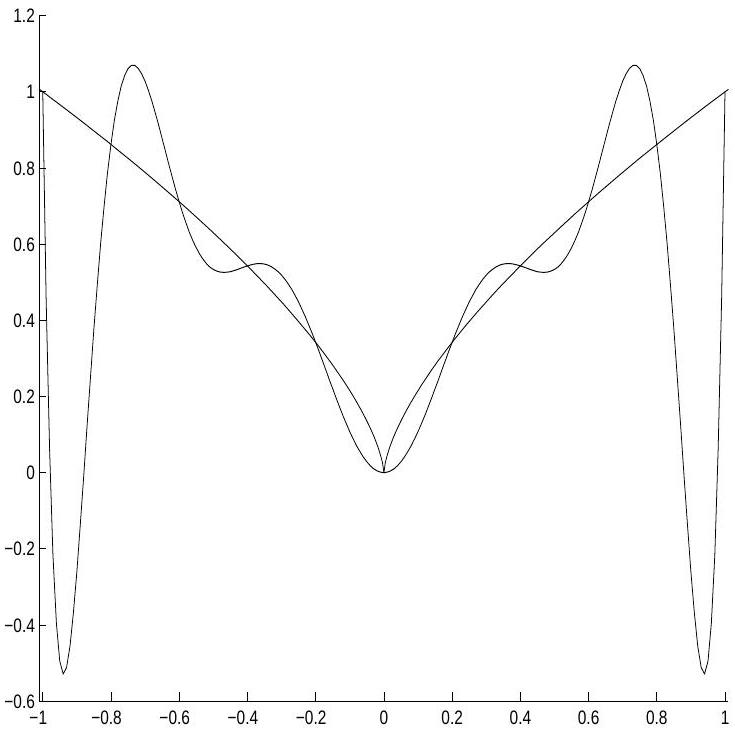
\includegraphics[width=\textwidth]{2025_09_05_3888c9ac96bd653d96b4g-096}
\captionsetup{labelformat=empty}
\caption{Figura 5.1. Interpolación de \$f(x)=x\^{}\{\textbackslash frac\{2}\{3\}\}\$ en $[-1,1]$, (11 puntos equiespaciados)\}\end{center}
\end{figure}

\section{Error de interpolación}
Cuando los datos obtenidos corresponden con datos de una función $f$ definida en $[a, b]$ y $x_{0}$, $x_{1}, \ldots, x_{n} \in[a, b]$ son $n+1$ puntos distintos, el polinomio interpolador a encontrar será un polinomio $p_{n} \in \mathcal{P}_{n}$ que coincida con $f$ en dichos puntos, es decir $p_{n}$ verifica que

$$
p_{n}\left(x_{j}\right)=f\left(x_{j}\right) \quad \forall j=0, \ldots, n .
$$

La ventaja de obtener un polinomio que interpola a una función $f$ de la cual sólo se conocen sus valores en los puntos $\left\{x_{0}, \ldots, x_{n}\right\}$ es que, el polinomio, arroja una fórmula que permite sustituir la función $f$ y hacer evaluaciones en puntos diferentes a los conocidos. Para que este\\
reemplazo tenga alguna validez numérica es importante conocer una estimación del error que se comete. Para esto será necesario suponer que la función $f$ verifica algunas condiciones de suavidad. Llamemos a este error:

$$
E_{n}(x)=f(x)-p_{n}(x), \quad x \in[a, b] .
$$

Con el siguiente teorema, damos el primer paso para poder estimar el error cometido; es decir, damos una expresión para $E_{n}(x)$.

Dados los puntos $x_{0}, \ldots, x_{n}$, utilizaremos la notación $W_{n+1}$ para designar al polinomio mónico de grado $n+1$ que se anula en esos puntos. Es decir,

$$
W_{n+1}(x)=\left(x-x_{0}\right) \cdots\left(x-x_{n}\right)
$$

Teorema 5.4. Sean $f \in C^{n+1}[a, b]$ y $p_{n} \in \mathcal{P}_{n}$ el polinomio interpolador de $f$ en $x_{0}, \ldots, x_{n}$ puntos del intervalo $[a, b]$. Para cada $x \in[a, b]$, existe $\xi \in[a, b], \xi=\xi(x)$, tal que

$$
E_{n}(x)=f(x)-p_{n}(x)=\frac{f^{(n+1)}(\xi)}{(n+1)!} W_{n+1}(x)
$$

Demostración. Notar que $E_{n}\left(x_{j}\right)=0$ y $W_{n+1}\left(x_{j}\right)=0$ para todo $j$. Por lo tanto, podemos suponer $x \neq x_{j}$. Fijado $x$ definimos la siguiente función de $t$,

$$
F(t)=f(t)-p_{n}(t)-\alpha W_{n+1}(t)
$$

donde $\alpha$ se elige de modo que $F(x)=0$. O sea, $\alpha=\frac{f(x)-p_{n}(x)}{W_{n+1}(x)}$, que está bien definida pues $W_{n+1}(x) \neq 0$. Observemos que para todo $j$,

$$
F\left(x_{j}\right)=f\left(x_{j}\right)-p_{n}\left(x_{j}\right)-\alpha W_{n+1}\left(x_{j}\right)=0
$$

Entonces $F$ se anula en los $n+2$ puntos $x_{0}, \ldots, x_{n}, x$. En consecuencia, por el teorema de Rolle, $F^{\prime}$ tiene al menos $n+1$ ceros, $F^{\prime \prime}$ al menos $n$ ceros y así siguiendo se tiene que existe un punto $\xi \in(a, b)$ tal que $F^{(n+1)}(\xi)=0$. Como

$$
F^{(n+1)}(t)=f^{(n+1)}(t)-(n+1)!\alpha
$$

Se obtiene,

$$
\frac{f^{(n+1)}(\xi)}{(n+1)!}=\frac{f(x)-p_{n}(x)}{W_{n+1}(x)}
$$

lo que concluye la demostración.

Ejemplo 5.5. Analicemos qué sucede si se quiere interpolar la función $f(x)=\cos (x)^{3}$ en el intervalo $[-3,3]$ por un polinomio.

Si se eligen 10 puntos equiespaciados se obtiene un polinomio como muestra la Figura 5.2. Si consideramos el error numérico, que es el que se obtiene como diferencia máxima entre $f$ y el polinomio evaluados en una malla suficientemente fina (puntos equiespaciados con paso $h=0,01$ ) se tiene un error de 0.4303 . . . Tan sólo al considerar 25 puntos equiespaciados (tomados a intervalos de longitud 0.25) se obtiene un error numérico menor que $10^{-6}$. En este caso, en una figura como la anterior, los gráficos del polinomio y la función se confunden.

\begin{figure}[h]
\begin{center}
  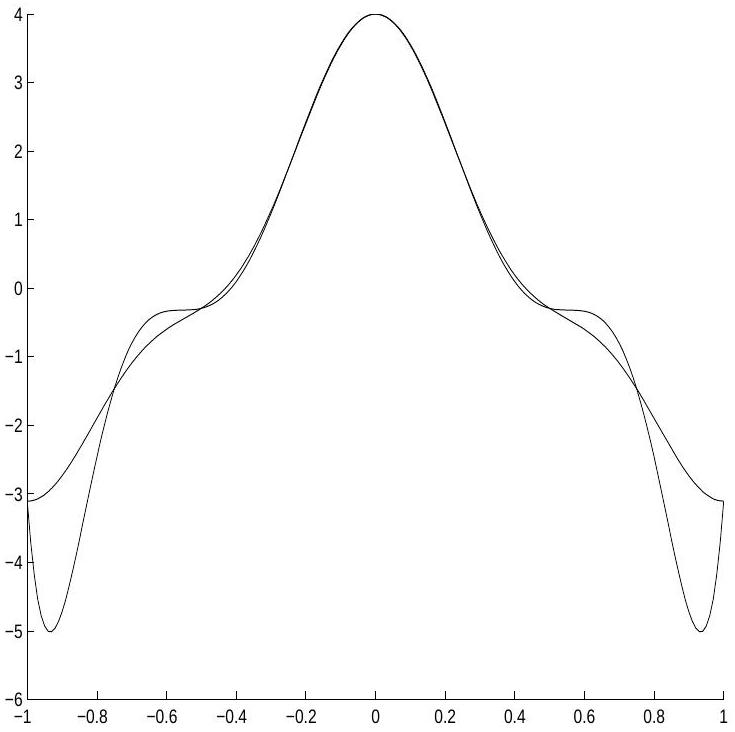
\includegraphics[width=\textwidth]{2025_09_05_3888c9ac96bd653d96b4g-098}
\captionsetup{labelformat=empty}
\caption{Figura 5.2. Interpolación de \$f(x)=\textbackslash cos (x)\^{}\{3}\$ en [-3,3], (10 puntos equiespaciados)\}\end{center}
\end{figure}

\section{Forma de Newton}
La forma de Newton es conveniente para calcular el polinomio, en $\mathcal{P}_{n}$, que interpola a una función $f$ en $x_{0}, \ldots, x_{n-1}, x_{n}$ una vez conocido el polinomio interpolador de $f$ en $x_{0}, \ldots, x_{n-1}$.

La forma de Newton del polinomio interpolador puede verse como una generalización del polinomio de Taylor asociado a una función. En esta construcción aparecen las diferencias divididas que presentamos a continuación.

\section*{Primera diferencia dividida}
$$
f\left[x_{0}, x_{1}\right]=\frac{f\left(x_{1}\right)-f\left(x_{0}\right)}{x_{1}-x_{0}} .
$$

\section*{Segunda diferencia dividida}
$$
f\left[x_{0}, x_{1}, x_{2}\right]=\frac{f\left[x_{1}, x_{2}\right]-f\left[x_{0}, x_{1}\right]}{x_{2}-x_{0}} .
$$

Así sucesivamente se define la diferencia de orden $k$ asociada a los puntos $x_{0}, \ldots, x_{k}$,

$$
f\left[x_{0}, \ldots, x_{k}\right]=\frac{f\left[x_{1}, \ldots, x_{k}\right]-f\left[x_{0}, \ldots, x_{k-1}\right]}{x_{k}-x_{0}} .
$$

La construcción de la forma de Newton se basa en la siguiente idea. Una vez obtenido $p_{k} \in \mathcal{P}_{k}$ que interpola a $f$ en $x_{0}, \ldots, x_{k}$ escribimos $p_{k+1} \in \mathcal{P}_{k+1}$ como

$$
p_{k+1}(x)=p_{k}(x)+a_{k+1}\left(x-x_{0}\right) \cdots\left(x-x_{k}\right) .
$$

Observemos que como el término agregado no modifica el valor de $p_{k}$ en $x_{0}, \ldots, x_{k}, p_{k+1}$ también interpola a $f$ en esos puntos independientemente del valor de $a_{k+1}$. Por otra parte, podemos elegir

$$
a_{k+1}=\frac{f\left(x_{k+1}\right)-p_{k}\left(x_{k+1}\right)}{\left(x_{k+1}-x_{0}\right) \cdots\left(x_{k+1}-x_{k}\right)}
$$

de modo que $p_{k+1}\left(x_{k+1}\right)=f\left(x_{k+1}\right)$.

Iterando este procedimiento desde $k=1$ hasta $k=n-1$ se obtiene la forma de Newton

$$
p_{n}(x)=a_{0}+a_{1}\left(x-x_{0}\right)+a_{2}\left(x-x_{0}\right)\left(x-x_{1}\right)+\ldots+a_{n}\left(x-x_{0}\right) \cdots\left(x-x_{n-1}\right)
$$

En lo que sigue veremos que los $a_{j}$ resultan ser las diferencias divididas y por lo tanto esta expresión es análoga al polinomio de Taylor.

Por ejemplo si $n=1$,

$$
p_{1}(x)=a_{0}+a_{1}\left(x-x_{0}\right)
$$

y como

$$
p_{1}\left(x_{0}\right)=f\left(x_{0}\right) \quad p_{1}\left(x_{1}\right)=f\left(x_{1}\right)
$$

tenemos

$$
a_{0}=f\left(x_{0}\right) \quad a_{1}=f\left[x_{0}, x_{1}\right]
$$

Si $n=2$,

$$
p_{2}(x)=a_{0}+a_{1}\left(x-x_{0}\right)+a_{2}\left(x-x_{0}\right)\left(x-x_{1}\right) .
$$

Como en el caso $n=1$, de las igualdades $p_{1}\left(x_{0}\right)=f\left(x_{0}\right)$ y $p_{1}\left(x_{1}\right)=f\left(x_{1}\right)$ queda

$$
a_{0}=f\left(x_{0}\right) \quad a_{1}=f\left[x_{0}, x_{1}\right] .
$$

Veamos ahora que

$$
a_{2}=f\left[x_{0}, x_{1}, x_{2}\right] .
$$

Sabemos ya que el polinomio $p_{1}(x)$ que interpola a $f$ en $x_{0}, x_{1}$ se escribe como

$$
p_{1}(x)=f\left(x_{0}\right)+f\left[x_{0}, x_{1}\right]\left(x-x_{0}\right) .
$$

Análogamente, si $q_{1}(x) \in \mathcal{P}_{1}$ interpola a $f$ en $x_{1}, x_{2}$ tenemos,

$$
q_{1}(x)=f\left(x_{1}\right)+f\left[x_{1}, x_{2}\right]\left(x-x_{1}\right) .
$$

Entonces, el polinomio

$$
r(x)=\frac{\left(x-x_{0}\right) q_{1}(x)-\left(x-x_{2}\right) p_{1}(x)}{x_{2}-x_{0}}
$$

tiene grado menor o igual que 2 y verifica $r\left(x_{j}\right)=f\left(x_{j}\right)$ para $j=0,1,2$. Por lo tanto, coincide con $p_{2}$.

En consecuencia, igualando los coeficientes de $x^{2}$ de $r$ y $p_{2}$ se obtiene

$$
a_{2}=\frac{f\left[x_{1}, x_{2}\right]-f\left[x_{0}, x_{1}\right]}{x_{2}-x_{0}}=f\left[x_{0}, x_{1}, x_{2}\right] .
$$

El mismo argumento puede aplicarse para demostrar el siguiente teorema.\\
Teorema 5.6. El polinomio $p_{n} \in \mathcal{P}_{n}$, que interpola a $f$ en los puntos $x_{0}, \ldots, x_{n}$ está dado por


\begin{equation*}
p_{n}(x)=f\left(x_{0}\right)+f\left[x_{0}, x_{1}\right]\left(x-x_{0}\right)+\cdots+f\left[x_{0}, \ldots, x_{n}\right]\left(x-x_{0}\right) \ldots\left(x-x_{n-1}\right) \tag{5.4}
\end{equation*}


No sólo los coeficientes del polinomio interpolador pueden expresarse en términos de las diferencias divididas, sino también el error como lo muestra el siguiente teorema.

Teorema 5.7. Si $p_{n} \in \mathcal{P}_{n}$ interpola a $f$ en los puntos $x_{0}, \ldots, x_{n}$, se tiene la siguiente expresión del error

$$
E_{n}(x)=f(x)-p_{n}(x)=f\left[x_{0}, \ldots, x_{n}, x\right] W_{n+1}(x) .
$$

Demostración. Agregamos $x_{n+1}$ a la sucesión $\left\{x_{0}, \ldots, x_{n}\right\}$ y consideramos $p_{n}$ y $p_{n+1}$ como en (5.4), entonces se tiene

$$
\begin{aligned}
p_{n+1}(x) & =f\left(x_{0}\right)+f\left[x_{0}, x_{1}\right]\left(x-x_{0}\right)+\cdots+f\left[x_{0}, \ldots, x_{n+1}\right]\left(x-x_{0}\right) \cdots\left(x-x_{n}\right) \\
& =p_{n}(x)+f\left[x_{0}, \ldots, x_{n+1}\right] W_{n+1}(x)
\end{aligned}
$$

Por lo tanto

$$
f\left(x_{n+1}\right)=p_{n+1}\left(x_{n+1}\right)=p_{n}\left(x_{n+1}\right)+f\left[x_{0}, \ldots, x_{n+1}\right] W_{n+1}\left(x_{n+1}\right) .
$$

De aquí se deduce que el error satisface

$$
E_{n}\left(x_{n+1}\right)=f\left(x_{n+1}\right)-p_{n}\left(x_{n+1}\right)=f\left[x_{0}, \ldots, x_{n+1}\right] W_{n+1}\left(x_{n+1}\right) .
$$

Como tomamos $x_{n+1}$ cualquier punto distinto de $x_{0}, \ldots, x_{n}$ se tiene para todo $x$,

$$
E_{n}(x)=f(x)-p_{n}(x)=f\left[x_{0}, \ldots, x_{n}, x\right] W_{n+1}(x)
$$

Corolario 5.8. Dados $x_{0}, \ldots, x_{n}$ puntos distintos, existe $\xi$ intermedio, es decir $\xi$ entre $x_{0}, \ldots, x_{n}$ tal que

$$
f\left[x_{0}, \ldots, x_{n}\right]=\frac{f^{(n)}(\xi)}{n!}
$$

Demostración. Evaluando en $x=x_{n}$ la expresión del error $E_{n-1}=f-p_{n-1}$, dada por el teorema anterior tenemos,

$$
E_{n-1}\left(x_{n}\right)=f\left[x_{0}, \ldots, x_{n}\right]\left(x_{n}-x_{0}\right) \cdots\left(x_{n}-x_{n-1}\right)
$$

lo que junto con la fórmula del error dada en el Teorema 5.4 concluye la demostración.

\section{Polinomios de Tchebychev - Minimización del Error}
Una pregunta natural es cómo elegir los puntos de interpolación para optimizar la aproximación. El Teorema 5.4 nos dice que el error depende de $f^{(n+1)}$ en algún punto del intervalo y de los puntos $x_{j}$ a través del polinomio $W_{n+1}(x)=\left(x-x_{0}\right)\left(x-x_{1}\right) \cdots\left(x-x_{n}\right)$. Como se pretende obtener una buena aproximación sin tener información sobre la función $f$, la idea es elegir los puntos de manera tal que $\left\|W_{n+1}(\cdot)\right\|_{\infty}$ sea mínima. Este problema, que en principio parece complicado, fue resuelto por Tchebychev en el siglo XIX introduciendo una sucesión de polinomios, que hoy llevan su nombre.

Para simplificar la presentación resolveremos el problema para funciones definidas en el intervalo $[-1,1]$. Más adelante veremos que se puede trasladar la construcción a cualquier intervalo $[a, b]$ mediante un cambio de variables.

Los polinomios de Tchebychev se definen para $k=0,1,2, \ldots$ por

$$
T_{k}(x)=\cos \left(k \cos ^{-1} x\right)
$$

donde $\cos ^{-1}$ es la inversa de $\cos :[0, \pi] \rightarrow[-1,1]$.\\
En principio no es evidente que $T_{k}$ sea un polinomio. Pero esto puede verse utilizando identidades trigonométricas. En efecto,

$$
T_{0}(x)=1, \quad T_{1}(x)=x
$$

y como $\cos (\alpha+\beta)+\cos (\alpha-\beta)=2 \cos \alpha \cos \beta$, si ponemos $x=\cos \theta$ resulta

$$
T_{k+1}(x)=\cos ((k+1) \theta)=2 \cos \theta \cos (k \theta)-\cos ((k-1) \theta),
$$

es decir,


\begin{equation*}
T_{k+1}(x)=2 x T_{k}(x)-T_{k-1}(x) . \tag{5.5}
\end{equation*}


Algunos ejemplos que siguen a $T_{0}$ y $T_{1}$ cuyos gráficos se muestran en la Figura 5.3 son

$$
\begin{array}{ll}
T_{2}(x)=2 x^{2}-1, & T_{4}(x)=8 x^{4}-8 x^{2}+1 \\
T_{3}(x)=4 x^{3}-3 x, & T_{5}(x)=16 x^{5}-20 x^{3}+5 x
\end{array}
$$

\begin{figure}[h]
\begin{center}
  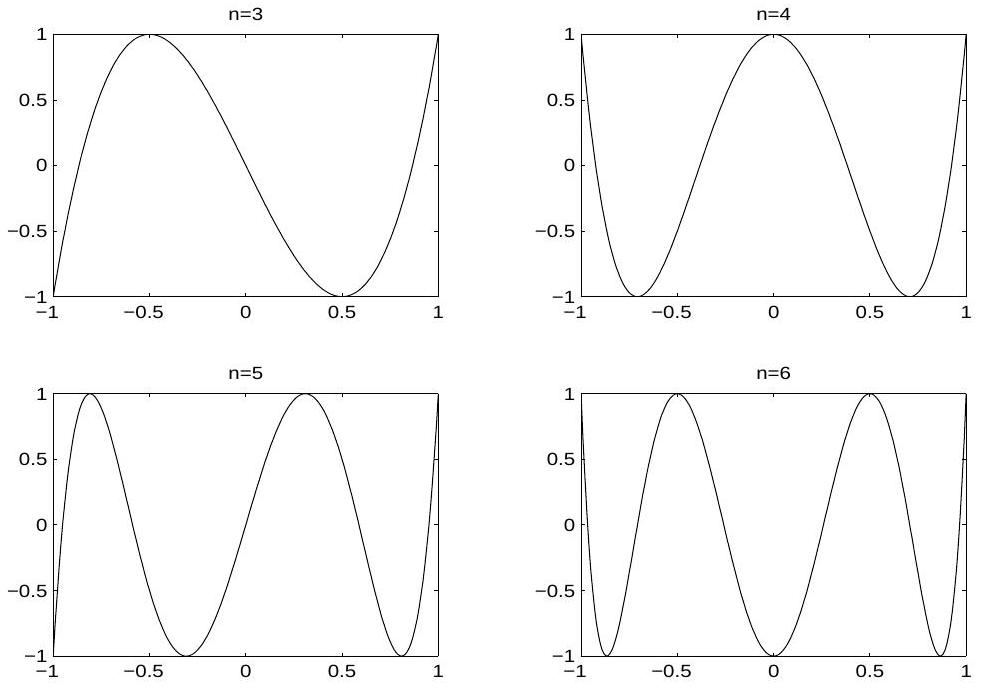
\includegraphics[width=\textwidth]{2025_09_05_3888c9ac96bd653d96b4g-102}
\captionsetup{labelformat=empty}
\caption{Figura 5.3. Polinomios de Tchebychev}
\end{center}
\end{figure}

Los polinomios de Tchebychev tienen las siguientes propiedades.\\
Proposición 5.9. Sea $T_{k}$ el polinomio de Tchebychev de grado $k$.

\begin{enumerate}
  \item El coeficiente principal de $T_{k}$ es $2^{k-1}$, para todo $k \in \mathbb{N}$.
  \item Las raíces del polinomio $T_{k}$ se encuentran en el intervalo $[-1,1]$ y son de la forma
\end{enumerate}

$$
x_{i}=\cos \left(\frac{(2 i+1) \pi}{2 k}\right)
$$

para $i=0,1, \ldots, k-1$. En particular, son todas distintas.\\
3. $\left\|T_{k}\right\|_{\infty}=1$. Además, $T_{k}$ alcanza los valores $1 y-1$ en $k+1$ puntos, es decir,

$$
\left\|T_{k}\right\|_{\infty}=\left|T_{k}\left(y_{i}\right)\right|=1 \quad \text { para } \quad y_{i}=\cos \left(\frac{i \pi}{k}\right)
$$

con $i=0, \ldots, k$.

Demostración. La primer afirmación puede verse de la relación de recurrencia (5.5).\\
Como $T_{k}(x)=\cos \left(k \cos ^{-1} x\right), T_{k}(x)=0$ si y sólo si el argumento es múltiplo impar de $\frac{\pi}{2}$. Es decir, para $i \in \mathbb{Z}$,

$$
\begin{aligned}
k \cos ^{-1}(x) & =(2 i+1) \frac{\pi}{2} \\
x & =\cos \left(\frac{(2 i+1)}{k} \frac{\pi}{2}\right)
\end{aligned}
$$

ambas afirmaciones de (2) quedan probadas. Es decir, las raíces pertenecen al intervalo $[-1,1]$ y variando los valores de $i=0,1, \ldots, k-1$ se obtienen todas.

Para probar (3), basta notar que $\left|T_{k}(x)\right| \leq 1$ por ser imagen de la función coseno. Además, sobre los puntos $y_{i}=\cos \left(\frac{i \pi}{k}\right), T_{k}$ toma alternativamente los valores $1,-1$ y por lo tanto la norma es exactamente 1.

Ahora sí, estamos en condiciones de enunciar y probar el resultado que anticipamos. Es decir, entre todas las posibles elecciones de $n+1$ puntos en $[-1,1]$, los ceros de $T_{n+1}$ son los puntos de interpolación que hay que elegir para minimizar la expresión $\left\|\left(x-x_{0}\right) \ldots\left(x-x_{n}\right)\right\|_{\infty}$ que aparece en la fórmula del error.\\
Teorema 5.10. Entre todos los polinomios mónicos de grado $n+1$,

$$
W_{n+1}(x)=\frac{1}{2^{n}} T_{n+1}(x)
$$

minimiza la norma $\left\|\|_{\infty}\right.$ en $[-1,1]$. O sea, si $P \in \mathcal{P}_{n+1}$ y es mónico entonces,

$$
\left\|W_{n+1}\right\|_{\infty} \leq\|P\|_{\infty}
$$

Demostración. Como el coeficiente principal de $T_{n+1}$ es $2^{n}$ se tiene que $W_{n+1}$ es mónico.\\
Supongamos que existe un polinomio $P \in \mathcal{P}_{n+1}$, mónico tal que

$$
\|P\|_{\infty}<\left\|W_{n+1}\right\|_{\infty} .
$$

Por la proposición anterior, $\left|W_{n+1}(x)\right|$ alcanza su máximo (que es $\frac{1}{2^{n}}$ ) en los $n+2$ puntos $y_{i}=\cos \left(\frac{i \pi}{n+1}\right), i=0, \ldots, n+1$. Esto es, si restringimos $W_{n+1}$ a $\left[y_{i}, y_{i+1}\right], W_{n+1}$ alcanza la norma infinito en cada uno de estos subintervalos. Entonces, en cada subintervalo se mantiene la relación


\begin{equation*}
\|P\|_{L^{\infty}\left[y_{i}, y_{i+1}\right]}<\frac{1}{2^{n}}=\left\|W_{n+1}\right\|_{L^{\infty}\left[y_{i}, y_{i+1}\right]} \tag{5.6}
\end{equation*}


Por otra parte, $W_{n+1}\left(y_{i}\right)=-W_{n+1}\left(y_{i+1}\right)$. Supongamos, por ejemplo, que $W_{n+1}\left(y_{i}\right)>0$ (en el caso contrario se procede de manera análoga). Entonces, de la desigualdad (5.6) se sigue que $P\left(y_{i}\right)<W_{n+1}\left(y_{i}\right)$ y que $P\left(y_{i+1}\right)>W_{n+1}\left(y_{i+1}\right)$.

Luego, el polinomio $Q(x)=P(x)-W_{n+1}(x)$ tiene al menos un cero en el intervalo ( $y_{i}, y_{i+1}$ ) y como hay $n+2$ valores de $y_{i}$, resulta que $Q$ tiene al menos $n+1$ ceros. Pero tanto $P$ como $W_{n+1}$ son polinomios de grado $n+1$ y ambos son mónicos de donde se deduce que $Q$ tiene grado a lo sumo $n$. Esto es una contradicción pues acabamos de ver que $Q$ tiene $n+1$ raíces distintas. Luego, un tal $P$ no puede existir.

Observación 5.11. Puede demostrarse, aunque no lo haremos aquí, que la desigualdad del teorema es estricta, o sea, $\left\|W_{n+1}\right\|_{\infty}<\|P\|_{\infty}$ si $P \neq W_{n+1}$ es un polinomio mónico $P \in \mathcal{P}_{n+1}$. Es decir el minimizante es único.\\
Ejemplo 5.12. Se quiere aproximar la función $f(x)=x^{\frac{2}{3}}$ en el intervalo $[-1,1]$ por un polinomio que la interpola en 11 puntos.

\begin{figure}[h]
\begin{center}
  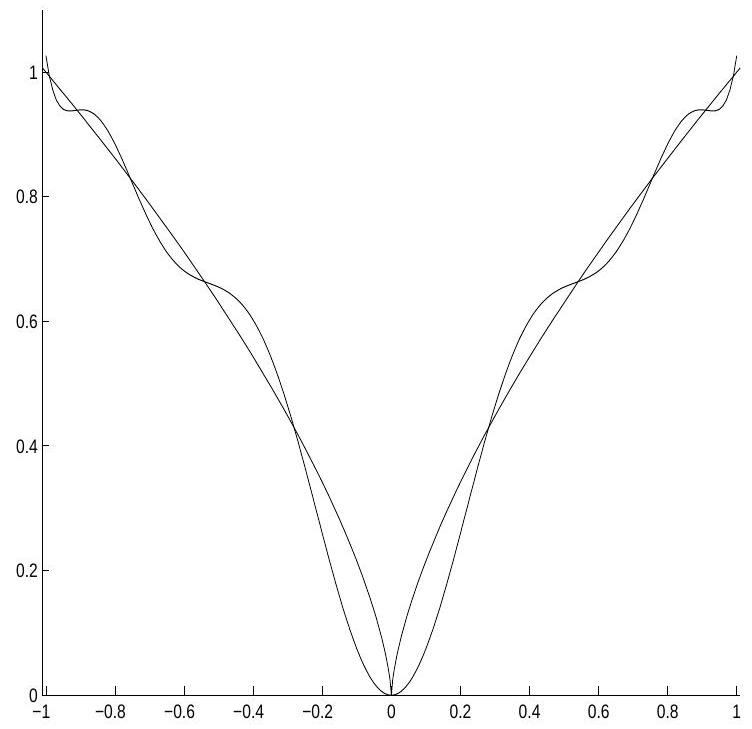
\includegraphics[width=\textwidth]{2025_09_05_3888c9ac96bd653d96b4g-104}
\captionsetup{labelformat=empty}
\caption{Figura 5.4. Interpolación de \$f(x)=x\^{}\{\textbackslash frac\{2}\{3\}\}\$ en los ceros de $T_{11}$\}\end{center}
\end{figure}

Si se eligen los nodos como los ceros de $T_{11}$ se obtiene un polinomio como muestra la Figura 5.4 (comparar con Figura 5.1). En este caso el error numérico cometido es menor que 0.1408, (comparar con Ejemplo 5.3).

Veamos ahora como se aplica el Teorema 5.7 para acotar el error cuando se usan las raíces de $T_{n+1}$ como puntos de interpolación.\\
Teorema 5.13. Sea $f \in C^{n+1}[-1,1]$. Si $p_{n} \in \mathcal{P}_{n}$ es el polinomio que interpola a $f$ en las raíces de $T_{n+1}$ entonces,

$$
\left\|f-p_{n}\right\|_{\infty} \leq \frac{\left\|f^{(n+1)}\right\|_{\infty}}{2^{n}(n+1)!}
$$

Demostración. Basta observar que $W_{n+1}=\frac{1}{2^{n}} T_{n+1}$ para obtener

$$
f(x)-p_{n}(x)=\frac{f^{(n+1)}(\xi)}{(n+1)!} W_{n+1}(x)=\frac{f^{(n+1)}(\xi)}{2^{n}(n+1)!} T_{n+1}(x),
$$

donde $\xi \in[-1,1]$. Entonces, el resultado se sigue del hecho de que $\left|T_{n+1}(x)\right| \leq 1$.

Ejemplo 5.14. Sea $f:[-1,1] \rightarrow \mathbb{R}$ dada por $f(x)=e^{3 x}$. Queremos comparar las cotas del error que se produce al estimar el valor de $f(0,8)$ al usar el polinomio interpolador de grado 4 construido con puntos equiespaciados y con los ceros del polinomio $T_{5}$.

Comencemos observando que $f^{(5)}(x)=243 e^{3 x}$ y por lo tanto

$$
\frac{\left\|f^{(5)}\right\|_{\infty}}{5!} \leq \frac{243 e^{3}}{5!} \leq \frac{4880,79}{5!}
$$

Si interpolamos $f$ en cinco puntos equiespaciados tenemos que

$$
W_{5}(x)=(x+1)(x+0,5) x(x-0,5)(x-1)
$$

entonces $\left|W_{5}(0,8)\right|=0,11232$ y usando la fórmula del error obtenemos

$$
\left|\left(f-p_{4}\right)(0,8)\right| \leq \frac{4880,79}{5!} 0,11232 \sim 4,57
$$

Cuando en realidad

$$
\left|E_{4}(0,8)\right|=0,4591 \ldots
$$

Notar que en este caso, se sobre estima el error en un factor de 10.\\
Ahora, interpolamos usando los ceros de $T_{4}$. La cota que se obtiene de la fórmula de error es

$$
\left|E_{4}(0,8)\right| \leq \frac{4880,79}{5!2^{4}}=2,54
$$

mientras que $E_{4}(0,8)=f(0,8)-p_{4}(0,8)=0,2544$.

Observemos que tanto el error como su estimación se reducen aproximadamente la mitad que en el caso de puntos equiespaciados.

ObSERVACIÓN 5.15. Una traslación lineal del intervalo $[a, b]$ al intervalo $[-1,1]$ nos permite dar los polinomios de Tchebychev correspondientes al intervalo $[a, b]$.

En efecto, es fácil ver que el cambio de variables $t=\frac{2(x-a)}{b-a}-1$ es la transformación mencionada. Por lo tanto

$$
\widetilde{T}_{k}(x)=T_{k}(t)=T_{k}\left(\frac{2(x-a)}{b-a}-1\right)=\cos \left(k \cos ^{-1}\left(\frac{2(x-a)}{b-a}-1\right)\right)
$$

es un polinomio de grado $k$ que tiene propiedades análogas a $T_{k}$ pero ahora en el intervalo $[a, b]$. En particular se tiene:

\begin{enumerate}
  \item La relación de recurrencia:
\end{enumerate}

$$
\widetilde{T}_{k+1}(x)=2\left(\frac{2(x-a)}{b-a}-1\right) \widetilde{T}_{k}(x)-\widetilde{T}_{k-1}(x)
$$

\begin{enumerate}
  \setcounter{enumi}{1}
  \item El coeficiente principal de $\widetilde{T}_{k}(x)$ es $2^{k-1}\left(\frac{2}{b-a}\right)^{k}$.
  \item Los ceros de $\widetilde{T}_{k}(x)$ son de la forma
\end{enumerate}

$$
x_{j}=\frac{b-a}{2} \cos \left(\frac{(2 j+1) \pi}{2 k}\right)+\frac{b+a}{2} \quad \forall j=0, \ldots, k-1 .
$$

\begin{enumerate}
  \setcounter{enumi}{3}
  \item Interpolando en los ceros de $\widetilde{T}_{n+1}$
\end{enumerate}

$$
W_{n+1}(x)=\frac{1}{2^{n}}\left(\frac{b-a}{2}\right)^{n+1} \widetilde{T}_{n+1}(x) \quad \text { у } \quad\left\|W_{n+1}\right\|_{\infty}=\frac{1}{2^{n}}\left(\frac{b-a}{2}\right)^{n+1}
$$

obteniéndose, para $x \in[a, b]$, la cota del error

$$
\left|f(x)-p_{n}(x)\right| \leq \frac{\left\|f^{(n+1)}\right\|_{\infty}}{(n+1)!2^{n}}\left(\frac{b-a}{2}\right)^{n+1}
$$

Antes de proceder con algunos comentarios finales estudiemos el análogo al Ejemplo 5.5 considerando como nodos los ceros del correspondiente polinomio de Tchebychev.

Ejemplo 5.16. Se quiere aproximar la función $f(x)=\cos (x)^{3}$ en el intervalo $[-3,3]$ por un polinomio que la interpola en los ceros de $T_{10}$.

Al elegirse como nodos los ceros de $T_{10}$ se obtiene un polinomio como muestra la Figura 5.5 (comparar con Figura 5.2). En este caso el error numérico cometido es menor que $4 \times 10^{-3}$. Comparar con Ejemplo 5.5 en el que se interpola la misma función en 10 puntos equiespaciados.

\begin{figure}[h]
\begin{center}
  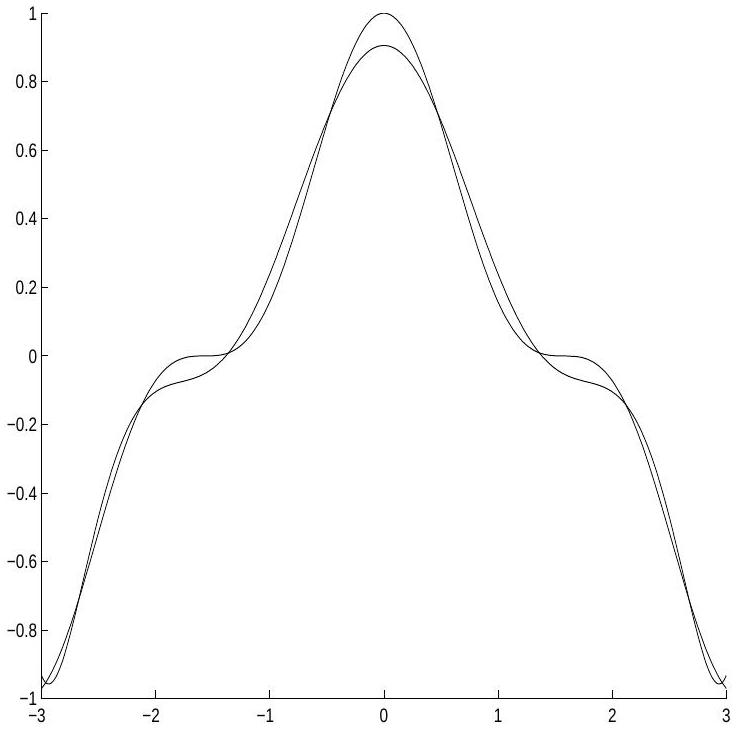
\includegraphics[width=\textwidth]{2025_09_05_3888c9ac96bd653d96b4g-107}
\captionsetup{labelformat=empty}
\caption{Figura 5.5. Interpolación de \$f(x)=\textbackslash cos (t)\^{}\{3}\$ en $[-3,3]$, (en los ceros de $T_{10}$ )\}\end{center}
\end{figure}

\section*{Comentarios:}
\begin{enumerate}
  \item A partir de la fórmula del error dada en el Teorema 5.4 puede demostrarse que si $f$ es una función entera, es decir, admite desarrollo de Taylor convergente en todo $\mathbb{R}$, entonces
\end{enumerate}

$$
\left\|f-p_{n}\right\|_{L^{\infty}[a, b]} \rightarrow 0 \quad(n \rightarrow \infty) .
$$

cualesquiera sean los puntos de interpolación.\\
2. No podemos asegurar convergencia uniforme, es decir, en norma infinito, si se cambia la hipótesis $f$ entera por $f \in C^{\infty}(\mathbb{R})$. Por ejemplo, si se eligen puntos equidistribuidos en el intervalo $[-1,1]$ se sabe que el error no tiende a cero para la función de Runge

$$
f(x)=\frac{1}{1+25 x^{2}}
$$

\begin{enumerate}
  \setcounter{enumi}{2}
  \item El comportamiento de la interpolación en los puntos de Tchebychev es mucho mejor. Por ejemplo, puede demostrarse que si la función $f$ es derivable
\end{enumerate}

$$
\left\|f-p_{n}\right\|_{\infty} \rightarrow 0 \quad(n \rightarrow \infty) .
$$

\begin{enumerate}
  \setcounter{enumi}{3}
  \item La interpolación en los puntos de Tchebychev no converge para cualquier función continua. O sea, puede verse que existe $f$ continua tal que $\left\|f-p_{n}\right\|_{\infty} \nrightarrow 0$. Más aún puede demostrarse el siguiente\\
Teorema. (Faber) Dados puntos
\end{enumerate}

$$
\begin{array}{cccc}
x_{0}^{0} & & & \\
x_{0}^{1} & x_{1}^{1} & & \\
x_{0}^{2} & x_{1}^{2} & x_{2}^{2} & \\
x_{0}^{3} & x_{1}^{3} & x_{2}^{3} & x_{3}^{3} \\
\vdots & & & \\
\vdots & & &
\end{array}
$$

arbitrarios en $[a, b]$, existe $f$ continua tal que $\left\|f-p_{n}\right\|_{\infty} \nrightarrow 0$, donde $p_{n}$ es el polinomio interpolador en $x_{0}^{n}, \ldots, x_{n}^{n}$.

\section{Interpolación de Hermite}
En algunos casos interesa también considerar junto con los valores de una función $f$ datos relacionados con sus derivadas. Por ejemplo, puede buscarse un polinomio $p$ que interpola a $f$ en determinados puntos y que además $p^{\prime}$ coincida con $f^{\prime}$ en algunos de esos puntos. Más en general, se tiene el siguiente teorema que fue probado por Hermite.

Teorema 5.17. Dada una función $f$, puntos $x_{0}, \ldots, x_{k}$ y $m_{0}, \ldots, m_{k} \in \mathbb{N}_{0}$ tales que $m_{0}+\ldots+ m_{k}=n+1$, existe un único polinomio $p \in \mathcal{P}_{n}$ que satisface

$$
\left\{\begin{array}{cccc}
p\left(x_{0}\right)=f\left(x_{0}\right), & p^{\prime}\left(x_{0}\right)=f^{\prime}\left(x_{0}\right), & \ldots & p^{\left(m_{0}-1\right)}\left(x_{0}\right)=f^{\left(m_{0}-1\right)}\left(x_{0}\right), \\
p\left(x_{1}\right)=f\left(x_{1}\right), & p^{\prime}\left(x_{1}\right)=f^{\prime}\left(x_{1}\right), & \ldots & p^{\left(m_{1}-1\right)}\left(x_{1}\right)=f^{\left(m_{1}-1\right)}\left(x_{1}\right), \\
\vdots & \vdots & & \vdots \\
p\left(x_{k}\right)=f\left(x_{k}\right), & p^{\prime}\left(x_{k}\right)=f^{\prime}\left(x_{k}\right), & \ldots & p^{\left(m_{k}-1\right)}\left(x_{k}\right)=f^{\left(m_{k}-1\right)}\left(x_{k}\right) .
\end{array}\right.
$$

No haremos una demostración de este teorema pero para dar una idea mostramos la construcción del polinomio interpolador en un caso particular; donde además puede verse cómo se generaliza la definición de diferencias divididas para valores de $x_{i}$ no todos distintos.

Se busca un polinomio $p \in \mathcal{P}_{3}$ que cumpla

$$
\begin{cases}(\text { i }) p\left(x_{0}\right)=f\left(x_{0}\right), & (\text { iii }) p\left(x_{1}\right)=f\left(x_{1}\right), \\ (\text { ii }) p^{\prime}\left(x_{0}\right)=f^{\prime}\left(x_{0}\right), & (\text { iv }) p^{\prime}\left(x_{1}\right)=f^{\prime}\left(x_{1}\right) .\end{cases}
$$

Como $\left\{1, x-x_{0},\left(x-x_{0}\right)^{2},\left(x-x_{0}\right)^{2}\left(x-x_{1}\right)\right\}$ forman una base de $\mathcal{P}_{3}$ por ser todos de distinto grado, cualquier polinomio en $\mathcal{P}_{3}$ se puede escribir de la forma

$$
p(x)=a_{0}+a_{1}\left(x-x_{0}\right)+a_{2}\left(x-x_{0}\right)^{2}+a_{3}\left(x-x_{0}\right)^{2}\left(x-x_{1}\right) .
$$

Las condiciones (i), (ii) se satisfacen si y sólo si $a_{0}=f\left(x_{0}\right)$ y $a_{1}=f^{\prime}\left(x_{0}\right)$. Ahora hay que determinar $a_{2}$ y $a_{3}$ para que se cumplan las dos condiciones restantes. Para simplificar la notación ponemos $h=\left(x_{1}-x_{0}\right)$, entonces se tiene

$$
p\left(x_{1}\right)=a_{0}+h a_{1}+h^{2} a_{2}=f\left(x_{0}\right)+f^{\prime}\left(x_{0}\right) h+a_{2} h^{2}
$$

Para que se satisfaga la condición (iii) debe ser

$$
a_{2}=\frac{f\left(x_{1}\right)-f\left(x_{0}\right)-f^{\prime}\left(x_{0}\right) h}{h^{2}}=\left(\frac{f\left(x_{1}\right)-f\left(x_{0}\right)}{h}-f^{\prime}\left(x_{0}\right)\right) \frac{1}{h} .
$$

Observemos que $\operatorname{lím}_{x_{1} \rightarrow x_{0}} f\left[x_{0}, x_{1}\right]=f^{\prime}\left(x_{0}\right)$ por lo que resulta natural generalizar la primer diferencia dividida poniendo

$$
f\left[x_{0}, x_{0}\right]=f^{\prime}\left(x_{0}\right)
$$

De esta manera se obtiene, de la definición de segunda diferencia dividida,

$$
f\left[x_{0}, x_{0}, x_{1}\right]=\frac{f\left[x_{0}, x_{1}\right]-f\left[x_{0}, x_{0}\right]}{x_{1}-x_{0}}=\left(\frac{f\left(x_{1}\right)-f\left(x_{0}\right)}{h}-f^{\prime}\left(x_{0}\right)\right) \frac{1}{h}
$$

y por lo tanto, $a_{2}=f\left[x_{0}, x_{0}, x_{1}\right]$.\\
Por último, queremos que $p^{\prime}\left(x_{1}\right)=f^{\prime}\left(x_{1}\right)$. Entonces, debemos elegir $a_{3}$ para que se cumpla

$$
f^{\prime}\left(x_{1}\right)=a_{1}+2 a_{2} h+a_{3} h^{2}=f^{\prime}\left(x_{0}\right)+2 f\left[x_{0}, x_{0}, x_{1}\right] h+a_{3} h^{2}
$$

de dónde,

$$
\begin{aligned}
a_{3} & =\frac{1}{h^{2}}\left(f^{\prime}\left(x_{1}\right)-f^{\prime}\left(x_{0}\right)-2 f\left[x_{0}, x_{0}, x_{1}\right] h\right) \\
& =\frac{1}{h^{2}}\left(f\left[x_{1}, x_{1}\right]-f\left[x_{0}, x_{0}\right]-2 f\left[x_{0}, x_{0}, x_{1}\right] h\right) \\
& =\frac{1}{h^{2}}\left(f\left[x_{1}, x_{1}\right]-f\left[x_{0}, x_{1}\right]+f\left[x_{0}, x_{1}\right]-f\left[x_{0}, x_{0}\right]-2 f\left[x_{0}, x_{0}, x_{1}\right] h\right) \\
& =\frac{1}{h}\left(f\left[x_{0}, x_{1}, x_{1}\right]+f\left[x_{0}, x_{0}, x_{1}\right]-2 f\left[x_{0}, x_{0}, x_{1}\right]\right) \\
& =\frac{f\left[x_{0}, x_{1}, x_{1}\right]-f\left[x_{0}, x_{0}, x_{1}\right]}{x_{1}-x_{0}}
\end{aligned}
$$

O sea

$$
a_{3}=f\left[x_{0}, x_{0}, x_{1}, x_{1}\right]
$$

En consecuencia, hemos demostrado que el único polinomio en $\mathcal{P}_{3}$ que satisface las condiciones pedidas es

$$
p_{3}(x)=f\left[x_{0}\right]+f\left[x_{0}, x_{0}\right]\left(x-x_{0}\right)+f\left[x_{0}, x_{0}, x_{1}\right]\left(x-x_{0}\right)^{2}+f\left[x_{0}, x_{0}, x_{1}, x_{1}\right]\left(x-x_{0}\right)^{2}\left(x-x_{1}\right) .
$$

Esto generaliza la forma de Newton para $x_{i}$ no todos distintos.

\section{Interpolación por polinomios a trozos}
En muchos casos para lograr una mejor aproximación es conveniente utilizar funciones polinomiales a trozos como interpolantes. De esta manera se parte el intervalo de manera tal que en cada subintervalo se elige un polinomio distinto que interpola los datos. Por ejemplo, al interpolar con polinomios de grado uno a trozos, quedan poligonales.

\begin{figure}[h]
\begin{center}
  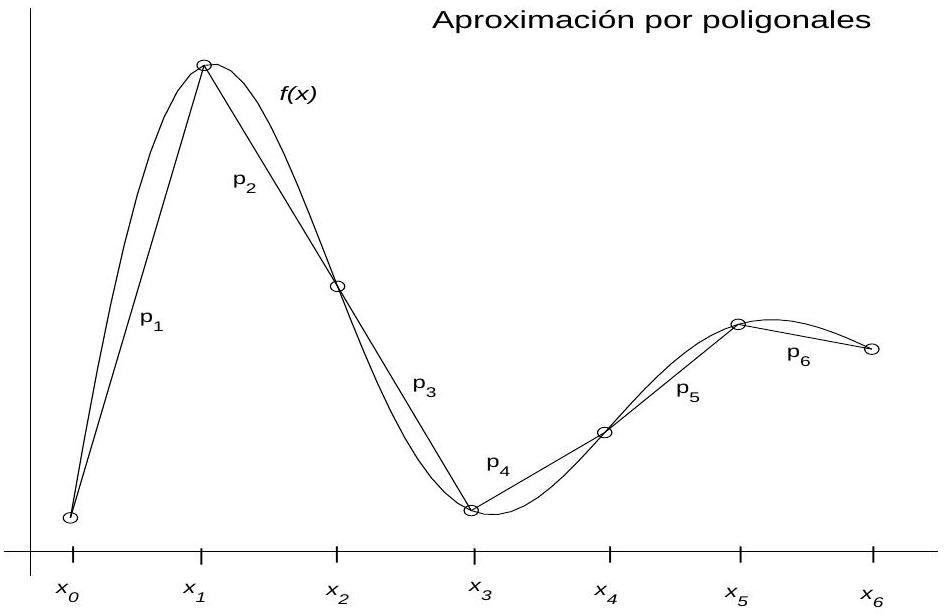
\includegraphics[width=\textwidth]{2025_09_05_3888c9ac96bd653d96b4g-110}
\captionsetup{labelformat=empty}
\caption{Figura 5.2}
\end{center}
\end{figure}

Partimos el intervalo $[a, b]$ en subintervalos $\left[x_{j}, x_{j+1}\right], a=x_{0}<x_{1}<x_{2} \ldots<x_{n}=b$. Dada $f:[a, b] \rightarrow \mathbb{R}$ definimos la función interpolante $q_{n}(x)$ tal que

$$
\left.q_{n}\right|_{\left[x_{j}, x_{j+1}\right]} \in \mathcal{P}_{1} .
$$

Consideremos el caso de puntos equiespaciados o sea, $x_{j}=a+j h$ con $h=\frac{b-a}{n}$. Para cualquier $f \in C^{2}[a, b]$ y cualquier $x \in\left[x_{j}, x_{j+1}\right]$, usando el Teorema 5.4 tenemos

$$
f(x)-q_{n}(x)=\frac{f^{\prime \prime}\left(\xi_{j}\right)}{2}\left(x-x_{j}\right)\left(x-x_{j+1}\right) .
$$

Entonces

$$
\left\|f-q_{n}\right\|_{\infty} \leq \frac{\left\|f^{\prime \prime}\right\|_{\infty}}{2} \frac{h^{2}}{4}=\frac{\left\|f^{\prime \prime}\right\|_{\infty}}{8} \frac{(b-a)^{2}}{n^{2}} \rightarrow 0
$$

cuando $n \rightarrow \infty$.\\
Ejemplo 5.18. Sea $f:[-1,1] \rightarrow \mathbb{R}$, la función de Runge $f(x)=\frac{1}{1+25 x^{2}}$. Puede verse que $\left\|f^{\prime \prime}\right\|_{\infty}=50$. En consecuencia, aproximando por poligonales obtenemos

$$
\left\|f-q_{n}\right\|_{\infty} \leq \frac{\left\|f^{\prime \prime}\right\|_{\infty}}{8}\left(\frac{2}{n}\right)^{2}=\frac{25}{n^{2}}
$$

Luego, en este caso, interpolando por poligonales obtenemos una aproximación mucho mejor que la que se obtiene interpolando con un polinomio, si se utilizan los mismos puntos.

\section*{Splines cúbicos.}
En muchos problemas interesa aproximar por funciones derivables. Esto no puede lograrse aproximando por poligonales y por lo tanto es necesario aumentar el grado de los aproximantes. Un método clásico es el correspondiente a grado tres, splines cúbicos. Vamos a ver que, de esta manera, puede obtenerse un aproximante $C^{2}$.

Dada $f \in C[a, b]$ y $a=x_{0}<x_{1}<x_{2} \ldots<x_{n}=b$ buscamos $S$ tal que $S, S^{\prime}$ y $S^{\prime \prime}$ sean continuas en $[a, b]$ y además se verifique

$$
S\left(x_{j}\right)=f\left(x_{j}\right) \quad \text { para } \quad 0 \leq j \leq n \quad \text { y }\left.\quad S\right|_{\left[x_{j}, x_{j+1}\right] \in \mathcal{P}_{3}}
$$

Por ejemplo si $n=3$, como $S_{j} \in \mathcal{P}_{3}$ tenemos $4 \times 3=12$ coeficientes a determinar. Veamos cuántas condiciones se tienen que satisfacer. Tenemos que verificar,

$$
\begin{array}{lll}
S_{0}\left(x_{0}\right)=f\left(x_{0}\right), & S_{1}\left(x_{1}\right)=f\left(x_{1}\right), & S_{2}\left(x_{2}\right)=f\left(x_{2}\right) \\
S_{0}\left(x_{1}\right)=S_{1}\left(x_{1}\right), & S_{1}\left(x_{2}\right)=S_{1}\left(x_{2}\right), & S_{2}\left(x_{3}\right)=f\left(x_{3}\right)
\end{array}
$$

es decir, seis condiciones. Si además queremos $S^{\prime}$ y $S^{\prime \prime}$ continuas en $x_{1}, x_{2}$ tenemos cuatro condiciones más. O sea, en total diez condiciones para doce incógnitas. Una cuenta análoga puede hacerse en el caso general para ver que la cantidad de coeficientes a determinar supera en dos al número de condiciones.

Luego, si hay solución habrá infinitas pues tenemos dos coeficientes para fijar arbitrariamente. Lo natural entonces es fijar $S^{\prime}\left(x_{0}\right)$ y $S^{\prime}\left(x_{n}\right)$ o bien $S^{\prime \prime}\left(x_{0}\right)$ y $S^{\prime \prime}\left(x_{n}\right)$. Elegiremos esta última opción por ser más simple.

Teorema 5.19. Dada $f \in C[a, b]$ y $a=x_{0}<x_{1}<x_{2} \ldots<x_{n}=b$, existe un única $S \in C^{2}[a, b]$ tal que

$$
\begin{cases}S\left(x_{j}\right)=f\left(x_{j}\right) & 0 \leq j \leq n \\ \left.S\right|_{\left[x_{j}, x_{j+1}\right]} \in \mathcal{P}_{3} & \end{cases}
$$

$\operatorname{con} S^{\prime \prime}(a)=S^{\prime \prime}(b)=0$.

Demostración. Para $j=0, \ldots, n-1$ usaremos la notación

$$
S_{j}=\left.S\right|_{\left[x_{j}, x_{j+1}\right]} \quad \text { у } \quad h_{j}=x_{j+1}-x_{j} .
$$

La función $S$ buscada debe cumplir que $S^{\prime \prime}$ es una poligonal. Por lo tanto, si $S^{\prime \prime}\left(x_{j}\right)=y_{j}, S_{j}^{\prime \prime}$ se escribe como

$$
S_{j}^{\prime \prime}(x)=y_{j} \frac{x_{j+1}-x}{h_{j}}+y_{j+1} \frac{x-x_{j}}{h_{j}} \quad 0 \leq j \leq n-1 .
$$

Veremos que es posible encontrar valores $y_{j}$ de tal forma que se cumplan las condiciones requeridas para $S$. Integrando dos veces obtenemos, para $x \in\left[x_{j}, x_{j+1}\right]$, con $0 \leq j \leq n-1$


\begin{equation*}
S_{j}(x)=\frac{y_{j}}{6 h_{j}}\left(x_{j+1}-x\right)^{3}+\frac{y_{j+1}}{6 h_{j}}\left(x-x_{j}\right)^{3}+c_{j}\left(x-x_{j}\right)+d_{j}\left(x_{j+1}-x\right) \tag{5.7}
\end{equation*}


donde $c_{j}, d_{j}$ son constantes a determinar que provienen de la integración.\\
Observemos que para cualquier elección de $y_{j}, c_{j}$ y $d_{j}, S^{\prime \prime}$ resulta continua por ser poligonal. Por lo tanto resta ver que esas constantes pueden elegirse de manera que se verifiquen las otras condiciones requeridas sobre $S$ y $S^{\prime}$.

Para que $S$ sea continua e interpole a $f$ tenemos que elegir $c_{j}, d_{j}$ tal que

$$
S_{j}\left(x_{j}\right)=f\left(x_{j}\right) \quad \text { y } \quad S_{j}\left(x_{j+1}\right)=f\left(x_{j+1}\right), \quad 0 \leq j \leq n-1
$$

de lo que, reemplazando en (5.7), obtenemos

$$
c_{j}=\frac{f\left(x_{j+1}\right)}{h_{j}}-\frac{y_{j+1} h_{j}}{6} \quad \text { у } \quad d_{j}=\frac{f\left(x_{j}\right)}{h_{j}}-\frac{y_{j} h_{j}}{6}
$$

y por lo tanto, para cada $0 \leq j \leq n-1$

$$
\begin{aligned}
S_{j}(x)= & \frac{y_{j}}{6 h_{j}}\left(x_{j+1}-x\right)^{3}+\frac{y_{j+1}}{6 h_{j}}\left(x-x_{j}\right)^{3}+ \\
& +\left(\frac{f\left(x_{j+1}\right)}{h_{j}}-\frac{y_{j+1} h_{j}}{6}\right)\left(x-x_{j}\right)+\left(\frac{f\left(x_{j}\right)}{h_{j}}-\frac{y_{j} h_{j}}{6}\right)\left(x_{j+1}-x\right) .
\end{aligned}
$$

Derivando, y utilizando la notación $\Delta f_{j}=f\left(x_{j+1}\right)-f\left(x_{j}\right)$, obtenemos

$$
S_{j}^{\prime}(x)=-\frac{y_{j}}{2 h_{j}}\left(x_{j+1}-x\right)^{2}+\frac{y_{j+1}}{2 h_{j}}\left(x-x_{j}\right)^{2}+\frac{\Delta f_{j}}{h_{j}}-\frac{h_{j}}{6}\left(y_{j+1}-y_{j}\right)
$$

y tenemos que elegir $y_{j}$ para que se cumpla la condición que falta, es decir, que $S^{\prime}$ sea continua, o sea

$$
S_{j}^{\prime}\left(x_{j}\right)=S_{j-1}^{\prime}\left(x_{j}\right) \quad 1 \leq j \leq n-1
$$

de lo que resulta que las $n+1$ incógnitas $y_{j}$ deben ser solución del siguiente sistema de $n-1$ ecuaciones,

$$
h_{j-1} y_{j-1}+2\left(h_{j}+h_{j-1}\right) y_{j}+h_{j} y_{j+1}=b_{j}
$$

con

$$
b_{j}=6\left(\frac{\Delta f_{j}}{h_{j}}-\frac{\Delta f_{j-1}}{h_{j-1}}\right)
$$

Como tenemos dos incógnitas más que ecuaciones, podemos dar valores arbitrarios a $y_{0}, y_{n} \mathrm{y}$, pasando los términos correspondientes al lado derecho, obtenemos el sistema tridiagonal,

$$
\left(\begin{array}{ccccc}
\gamma_{1} & h_{1} & 0 & \cdots & 0 \\
h_{1} & \gamma_{2} & h_{2} & \cdots & 0 \\
\vdots & \vdots & & \ddots & \vdots \\
0 & \cdots & & \cdots & \gamma_{n-1}
\end{array}\right)\left(\begin{array}{c}
y_{1} \\
y_{2} \\
\vdots \\
y_{n-1}
\end{array}\right)=\left(\begin{array}{c}
b_{1}-h_{0} y_{0} \\
b_{2} \\
\vdots \\
b_{n-1}-h_{n-1} y_{n}
\end{array}\right)
$$

donde $\gamma_{i}=2\left(h_{i}+h_{i-1}\right)$.\\
Ahora, como $A$ es diagonal estrictamente dominante, entonces es inversible. Por lo tanto existe solución única una vez elegidos $y_{0}, y_{n}$.

Por ejemplo podemos elegir $y_{0}=y_{n}=0$ para que se satisfagan las condiciones $S^{\prime \prime}\left(x_{0}\right)=0$ y $S^{\prime \prime}\left(x_{n}\right)=0$, lo que concluye la demostración.

Observemos que en general $S^{\prime}\left(x_{j}\right) \neq f^{\prime}\left(x_{j}\right)$ y $S^{\prime \prime}\left(x_{j}\right) \neq f^{\prime \prime}\left(x_{j}\right)$.

\section{Ejercicios}
\begin{enumerate}
  \item Para cada uno de los conjuntos de datos dados en las siguientes tablas calcular el polinomio $p(x)$ interpolador de grado menor o igual que 3, en la forma de Lagrange. Verificar utilizando el comando polyfit de Matlab. Graficar el polinomio interpolador, usando el comando polyval.
\end{enumerate}

\begin{center}
\begin{tabular}{l|l|l|l|l|}
\hline
x & -1 & 0 & 2 & 3 \\
y & -1 & 3 & 11 & 27 \\
\hline
\end{tabular}
\end{center}

\begin{center}
\begin{tabular}{|l|l|l|l|l|}
\hline
x & -1 & 0 & 1 & 2 \\
y & -3 & 1 & 1 & 3 \\
\hline
\end{tabular}
\end{center}

\begin{enumerate}
  \setcounter{enumi}{1}
  \item Repetir el problema anterior, usando el método de coeficientes indeterminados.
  \item a) Construir las tablas de diferencias divididas para los datos del Ejercicio 1, y emplearlas para construir los polinomios interpoladores.\\
b) Agregar a las tablas de datos del Ejercicio 1 el punto $x=4, y=1$. Aumentar las tablas de diferencias divididas y calcular los polinomios interpoladores.
  \item Considerar la función $f(x)=\frac{1}{1+25 x^{2}}$ en el intervalo $[-1,1]$. Graficar $f$ junto con los polinomios que resultan de interpolar a $f$ en los $n+1$ puntos equiespaciados $x_{0}= -1, \ldots, x_{i}=x_{0}+\frac{2 i}{n}, \ldots, x_{n}=1 ;$ para $n=5,10,15$.
  \item Repetir el Ejercicio 4 para la función $f_{1}:[-1,1] \rightarrow \mathbb{R}, f_{1}(x)=|x|$ y para la función $f_{2}:[-1,1] \rightarrow \mathbb{R}, f_{2}(x)=\operatorname{sen}(\pi x)$.
  \item Sea $f:[0,5] \rightarrow \mathbb{R}, f(x)=2^{x}$. Sea $P_{n}$ un polinomio de grado $n$ que interpola a $f$ en $n+1$ puntos distintos cualesquiera de dicho intervalo. Demostrar que para todo $x \in[0,5]$,
\end{enumerate}

$$
\left|P_{n}(x)-f(x)\right| \leq \frac{32,5^{n+1}}{(n+1)!}
$$

\begin{enumerate}
  \setcounter{enumi}{6}
  \item Sea $f$ una función $C^{\infty}$ tal que para todo $k \in \mathbb{N}$ y para todo $x \in[a, b]$ se tiene:
\end{enumerate}

$$
\left|f^{(k)}(x)\right| \leq C^{k} k!
$$

Mostrar que, si $0<C<\frac{1}{b-a}$ y $P_{n}$ en un polinomio de grado $n$ que interpola a $f$ en $n+1$ puntos distintos, entonces $P_{n}$ converge a $f$ uniformemente, es decir, $\left\|f-P_{n}\right\|_{\infty} \rightarrow 0$ cuando $n$ tiende a $\infty$.\\
8. Sea $f:[-1,1] \rightarrow \mathbb{R}, f(x)=\frac{1}{a+x}$. Sean $\left(x_{n}\right)_{n \geq 0}$ una sucesión arbitraria de puntos en $[-1,1]$ y $P_{n}(x)$ el polinomio que interpola a $f(x)$ en $x_{0}, x_{1}, \ldots, x_{n}$. Demostrar que si $a>3$ entonces $P_{n}$ converge a $f$ uniformemente.\\
9. a) Dado el intervalo $[a, b]$, sea $m$ el punto medio entre $a$ y $b$ y sea $h \leq(b-a) / 2$. Sea $p=m-h$ y $q=m+h$. Demostrar que para todo $x$ en $[a, b]$,

$$
|(x-p)(x-q)| \leq \frac{(b-a)^{2}}{4}
$$

b) Sean $x_{0}=a, \ldots, x_{i}=x_{0}+\frac{b-a}{n}, \ldots, x_{n}=b, n+1$ puntos equiespaciados en el intervalo $[a, b]$. Demostrar que para todo $x$ en $[a, b]$,

$$
\left|\left(x-x_{0}\right) \ldots\left(x-x_{n}\right)\right| \leq \frac{(b-a)^{n+1}}{2^{n+1}}
$$

\begin{enumerate}
  \setcounter{enumi}{9}
  \item Sea $f:[-\pi, \pi] \rightarrow \mathbb{R}, f(x)=\operatorname{sen}(x)$. Sea $P_{n}$ un polinomio de grado $n$ que interpola a $f$ en $n+1$ puntos equiespaciados en dicho intervalo.\\
a) Demostrar que para todo $x \in[-\pi, \pi]$
\end{enumerate}

$$
\left|P_{n}(x)-f(x)\right| \leq \frac{\pi^{n+1}}{(n+1)!}
$$

b) Concluir que $P_{n}$ converge uniformemente a $f$.\\
11. Sea $f:[0,1] \rightarrow \mathbb{R}, f(x)=\operatorname{sen}(\pi x)+e^{x}$. Sea $P_{n}$ el polinomio de grado $n$ que interpola a $f$ en $n+1$ puntos equiespaciados.\\
a) Usando el ejercicio 9 , acotar el error $\left\|f-P_{n}\right\|_{\infty}$.\\
b) Sea $C_{n}$ la cota hallada en (a). Para $n=1,3,5$ graficar simultáneamente $f, f+C_{n}$, $f-C_{n}$ y $P_{n}$.\\
12. Calcular el grado mínimo $n$ que debe tener un polinomio $P_{n}$ que interpola en los ceros de $T_{n+1}$ a la función $f(x)=e^{2 x}, x \in[-1,1]$, para que el error $\left\|f-P_{n}\right\|_{\infty} \leq 10^{-2}$.\\
13. Repetir el ejercicio anterior para $f(x)=e^{x}, x \in[0,4]$.\\
14. Para $n=5,10,15$; graficar simultáneamente el polinomio $W_{n+1}(x)=\prod_{i=0}^{n}\left(x-x_{i}\right)$, donde $x_{i}=-1+2 i / n ; i=0, \ldots, n$ y el polinomio de Tchebychev $T_{n+1}$.\\
15. Repetir los Ejercicios 4 y 5 usando los polinomios que interpolan a la función $f$ en los ceros del polinomio de Tchebychev de grado $n+1$, para $n=5,10,15$.\\
16. Utilizar el método de coeficientes indeterminados para hallar un polinomio $p$ de grado 2 que satisfaga:

$$
p(1)=0, \quad p^{\prime}(1)=7, \quad p(2)=10
$$

\begin{enumerate}
  \setcounter{enumi}{16}
  \item a) Sea $f(x)=\cos (\pi x)$, hallar un polinomio de grado menor o igual que 3 que verifique
\end{enumerate}

$$
p(-1)=f(-1), p(0)=f(0), p(1)=f(1), p^{\prime}(1)=f^{\prime}(1) .
$$

b) Hallar un polinomio de grado menor o igual que 4 que verifique las condiciones del item anterior, más la condición

$$
p^{\prime \prime}(1)=f^{\prime \prime}(1) .
$$

\begin{enumerate}
  \setcounter{enumi}{17}
  \item Sea $f:[-1,1] \rightarrow \mathbb{R}$ la función $f(x)=e^{2 x-1}$ y sean $x_{0}<x_{1}<\ldots<x_{n}$ los ceros del polinomio de Tchebychev, $T_{n+1}$. Se interpola a $f$ con un polinomio $P$ de grado $\leq n+1$ de modo que $P\left(x_{0}\right)=f\left(x_{0}\right), P\left(x_{1}\right)=f\left(x_{1}\right), \ldots, P\left(x_{n}\right)=f\left(x_{n}\right)$ y además $P^{\prime}\left(x_{n}\right)=f^{\prime}\left(x_{n}\right)$. Probar que si $n \geq 6$ entonces, el error cometido en la interpolación sobre el intervalo $[-1,1]$ es menor que $10^{-3}$.
  \item Para ilustrar qué pasa cuando se desea interpolar no sólo una función sino también sus derivadas, consideramos el problema de hallar $p$ de grado a lo sumo 3 que verifique:\\
(a) $\quad p(0)=1, \quad p^{\prime}(0)=1, \quad p^{\prime}(1)=2, \quad p(2)=1 ;$\\
(b) $\quad p(-1)=1, \quad p^{\prime}(-1)=1, \quad p^{\prime}(1)=2, \quad p(2)=1$;\\
(c) $\quad p(-1)=1, \quad p^{\prime}(-1)=-6, \quad p^{\prime}(1)=2, \quad p(2)=1$.
\end{enumerate}

Usando el método de coeficientes indeterminados, demostrar que el problema (a) tiene solución única, el problema (b) no tiene solución, y el problema (c) tiene infinitas soluciones.\\
20. Analizar para qué valores de $x_{0}, x_{1}, x_{2}$, y $\alpha_{0}, \alpha_{1}, \alpha_{2}$ existe un polinomio de grado 2 que satisface:

$$
p\left(x_{0}\right)=\alpha_{0}, p\left(x_{1}\right)=\alpha_{1}, p^{\prime}\left(x_{2}\right)=\alpha_{2} .
$$

\begin{enumerate}
  \setcounter{enumi}{20}
  \item Sea $f \in C^{2}[a, b]$, y sean $x_{0}=a, x_{1}=a+h, \ldots, x_{n}=b$, donde $h=(b-a) / n$. Considerar la poligonal $l(x)$ que interpola a $f$ en los puntos $x_{i}, i=0 \ldots n$. Probar que\\
a)
\end{enumerate}

$$
|f(x)-l(x)| \leq \frac{h^{2}}{2} \operatorname{máx}_{x \in[a, b]}\left|f^{\prime \prime}(x)\right|
$$

b)

$$
\left|f^{\prime}(x)-l^{\prime}(x)\right| \leq h \operatorname{máx}_{x \in[a, b]}\left|f^{\prime \prime}(x)\right|
$$

\begin{enumerate}
  \setcounter{enumi}{21}
  \item a) Determinar valores de $\alpha, \beta$ y $\gamma$ en $\mathbb{R}$ para que $S$ sea una función spline cúbica, siendo:
\end{enumerate}

$$
S(x)= \begin{cases}\alpha x^{3}+\gamma x, & 0 \leq x \leq 1 \\ -\alpha x^{3}+\beta x^{2}-5 \alpha x+1, & 1 \leq x \leq 2\end{cases}
$$

b) Con los valores de $\alpha, \beta$ y $\gamma$ obtenidos en el ítem anterior, decidir si $S$ interpola a la función $f(x)=2^{x}+0,5 x^{2}-0,5 x-1,0 \leq x \leq 2$ respecto de la partición $\{0,1,2\}$.\\
c) Graficar simultáneamente $f$ y $S$ en el intervalo $[0,2]$.\\
23. Sea $f$ como en el Ejercicio 4. Utilizando Matlab, graficar la función $f$ junto con una spline cúbica que la interpola en la red $\{-1,-0,75, \ldots, 0,75,1\}$, tomando como condiciones de borde las derivadas de $f$.\\
24. Encontrar una función del tipo $2^{a x^{3}+b x^{2}+c x+d}$ que interpole la siguiente tabla de datos:

\begin{center}
\begin{tabular}{|c|c|c|c|c|}
\hline
$x$ & -1 & 0 & 1 & 2 \\
\hline
$y$ & 1 & 1 & 0.5 & 4 \\
\hline
\end{tabular}
\end{center}

\begin{enumerate}
  \setcounter{enumi}{24}
  \item Utilizando Matlab, encontrar y graficar una función del tipo $e^{a_{4} x^{4}+a_{3} x^{3}+\cdots+a_{0}}$ que interpole a la función $f(x)=1 / x$ en 5 nodos equiespaciados en el intervalo $[1,10]$.
\end{enumerate}

\chapter{Polinomios ortogonales y aproximación por cuadrados mínimos}
En el capítulo anterior hemos discutido cómo aproximar una función por polinomios que interpolan a la función misma y/o a sus derivadas en algunos puntos. Hasta ahora, los métodos analizados nos permiten construir polinomios de grado $n$ a partir de $n+1$ datos. Cierto es que, en un problema a modelizar, cuantos más datos se conocen es de esperar que se pueda lograr mayor precisión. Pero, como vimos, muchas veces polinomios de alto grado producen efectos no deseados como por ejemplo grandes oscilaciones. En este capítulo consideraremos otra forma de aproximar funciones conocida como el método de cuadrados mínimos. Este método nos permitirá, cuando se trate de aproximar por polinomios, contemplar una tabla de valores sin sujetar el grado del polinomio a la cantidad de datos. También será posible considerar funciones más generales que ajusten de manera natural los valores predeterminados.

En general, en esta clase de problemas uno sabe a priori a qué tipo de función corresponden los datos. Una situación frecuente es la de aproximar una tabla de más de dos valores por una recta (como muestra la Figura 6.1). Es decir, se tienen valores $\left(x_{i}, y_{i}\right), i=0, \ldots, n$ y se quiere encontrar una recta que ajuste estos datos lo mejor posible. Si escribimos la ecuación de la recta como $y=m x+b$ nuestro problema consiste en encontrar valores de $m$ y $b$ que hagan que el error $\left|y_{i}-\left(m x_{i}+b\right)\right|$ sea lo mas chico posible para todo $i$. Por ejemplo, una manera de lograr esto sería pedir que $m$ y $b$ minimicen

$$
\operatorname{máx}_{0 \leq i \leq n}\left|y_{i}-\left(m x_{i}+b\right)\right|
$$

o también podríamos pedir que minimicen

$$
\sum_{i=0}^{n}\left|y_{i}-\left(m x_{i}+b\right)\right| \quad \text { о } \quad \sum_{i=0}^{n}\left|y_{i}-\left(m x_{i}+b\right)\right|^{2} .
$$

De todas estas opciones es usual considerar la última, llamada "aproximación por cuadrados mínimos", debido a que es la más simple ya que el problema se reduce a resolver ecuaciones lineales.

En este capítulo estudiaremos distintos métodos para resolver éste y otros problemas. Como en general los valores de $y_{i}$ corresponden a datos de una función $f$, podemos plantear estos problemas en el contexto de aproximación de funciones. Dada una función $f$ consideramos:

\begin{figure}[h]
\begin{center}
  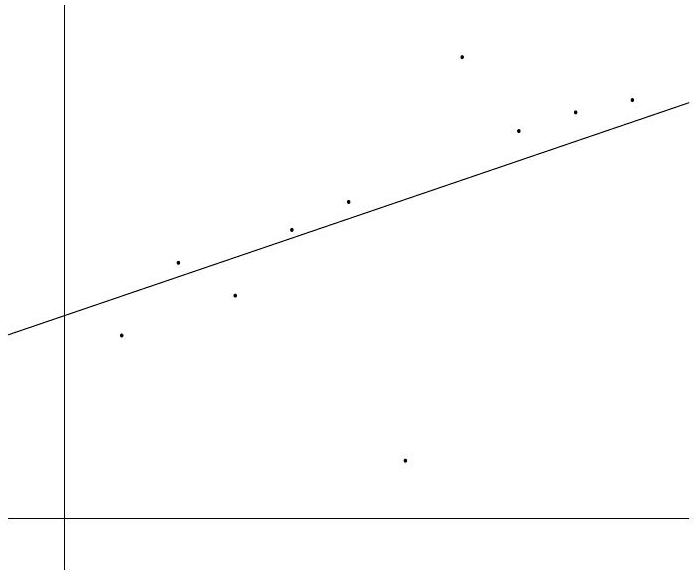
\includegraphics[width=\textwidth]{2025_09_05_3888c9ac96bd653d96b4g-118}
\captionsetup{labelformat=empty}
\caption{Figura 6.1. Aproximación de 10 valores por una recta}
\end{center}
\end{figure}

Problema A. Dados $w_{0}, \ldots, w_{n}$ constantes positivas ( pesos ), $m<n$ y valores ( $x_{i}, f\left(x_{i}\right)$ ), con $i=0, \ldots, n$ se trata de hallar $p \in \mathcal{P}_{m}$ que minimice

$$
\sum_{i=0}^{n} w_{i}\left(p\left(x_{i}\right)-f\left(x_{i}\right)\right)^{2} .
$$

Problema B. Dada $w(x)$ una función positiva en $[a, b]$, dada $f$ y $m \in \mathbb{N}$ se trata de hallar $p \in \mathcal{P}_{m}$ que minimice

$$
\int_{a}^{b} w(x)(f(x)-p(x))^{2} d x
$$

\section{Preliminares}
Nos dedicaremos especialmente al estudio de aproximaciones por polinomios. Comenzamos esta sección presentando un resultado clásico de Weierstrass que muestra que toda función continua puede aproximarse uniformemente por polinomios, en todo intervalo cerrado y acotado.

Teorema 6.1. (Weierstrass) Sea $f \in C[a, b]$. Para todo $\varepsilon>0$ existe un polinomio $p$ tal que

$$
\|f-p\|_{\infty}<\varepsilon
$$

Demostración. Damos la demostración para el intervalo [ 0,1 ], el caso general se obtiene fácilmente mediante un cambio de variables.

Definimos los polinomios de Bernstein,

$$
B_{n} f(x)=\sum_{k=0}^{n}\binom{n}{k} f\left(\frac{k}{n}\right) x^{k}(1-x)^{n-k}
$$

y vamos a demostrar que $B_{n} f$ converge uniformemente a $f$ en el intervalo $[0,1]$. Para eso necesitaremos calcular $B_{n} h_{j}$ para $h_{j}(x)=x^{j}, j=0,1,2$.

Usando la fórmula del binomio de Newton, se tiene:

$$
\begin{aligned}
B_{n} h_{0}(x) & =\sum_{k=0}^{n}\binom{n}{k} x^{k}(1-x)^{n-k}=(x+1-x)^{n}=1 . \\
B_{n} h_{1}(x) & =\sum_{k=0}^{n}\binom{n}{k} \frac{k}{n} x^{k}(1-x)^{n-k}=\sum_{k=1}^{n}\binom{n-1}{k-1} x^{k}(1-x)^{n-k} \\
& =x \sum_{k=1}^{n}\binom{n-1}{k-1} x^{k-1}(1-x)^{n-k}=x(x+1-x)^{n-1}=x . \\
B_{n} h_{2}(x) & =\sum_{k=0}^{n}\binom{n}{k}\left(\frac{k}{n}\right)^{2} x^{k}(1-x)^{n-k}=\sum_{k=0}^{n}\binom{n-1}{k-1} \frac{k}{n} x^{k}(1-x)^{n-k} \\
& =\sum_{k=0}^{n}\binom{n-1}{k-1}\left(\frac{n-1}{n} \frac{k-1}{n-1}+\frac{1}{n}\right) x^{k}(1-x)^{n-k} \\
& =\frac{n-1}{n} x^{2} \sum_{k=2}^{n}\binom{n-2}{k-2} x^{k-2}(1-x)^{n-k}+\frac{x}{n} \\
& =\frac{n-1}{n} x^{2}(x+1-x)^{n-2}+\frac{x}{n}=x^{2}+\frac{x(1-x)}{n} .
\end{aligned}
$$

Dado $y \in \mathbb{R}$ consideremos la función $g_{y}(x)=(x-y)^{2}$. Desarrollando $(x-y)^{2}=x^{2}-2 x y+y^{2}$ y usando que $B_{n}$ es lineal (o sea, $B_{n}\left(f_{1}+f_{2}\right)=B_{n} f_{1}+B_{n} f_{2}$ y $B_{n}(k f)=k B_{n} f$ ) se obtiene


\begin{equation*}
B_{n} g_{y}(x)=g_{y}(x)+\frac{x(1-x)}{n} . \tag{6.1}
\end{equation*}


Por otra parte, como toda función continua en un intervalo cerrado es uniformemente continua, dado $\varepsilon>0$, existe $\delta>0$ tal que,

$$
|f(x)-f(y)| \leq \varepsilon \quad \text { si } \quad|x-y|<\delta .
$$

Además, para los $x, y$ tales que $|x-y| \geq \delta$ se tiene

$$
|f(x)-f(y)| \leq 2\|f\|_{\infty} \leq \frac{2\|f\|_{\infty}}{\delta^{2}}(x-y)^{2}
$$

Luego, para todo $x, y$, podemos asegurar que,

$$
|f(x)-f(y)| \leq \varepsilon+\frac{2\|f\|_{\infty}}{\delta^{2}}(x-y)^{2}
$$

es decir,

$$
-\varepsilon-\frac{2\|f\|_{\infty}}{\delta^{2}}(x-y)^{2} \leq f(x)-f(y) \leq \varepsilon+\frac{2\|f\|_{\infty}}{\delta^{2}}(x-y)^{2} .
$$

Ahora, si $f_{1} \leq f_{2}$, de la definición de $B_{n}$ puede verse que $B_{n} f_{1} \leq B_{n} f_{2}$; esto es $B_{n}$ preserva el orden. En consecuencia, aplicando $B_{n}$ en la desigualdad anterior, teniendo en cuenta (6.1), y recordando que $B_{n}$ es lineal y que $B_{n} 1=1$ se obtiene (tener presente que hasta aquí estamos considerando $y$ como una constante),

$$
\left|B_{n} f(x)-f(y)\right| \leq \varepsilon+\frac{2\|f\|_{\infty}}{\delta^{2}}(x-y)^{2}+\frac{2\|f\|_{\infty}}{\delta^{2}} \frac{x(1-x)}{n}
$$

y por lo tanto, evaluando ambos lados de la desigualdad en $y$, resulta

$$
\left|B_{n} f(y)-f(y)\right| \leq \varepsilon+\frac{2\|f\|_{\infty}}{\delta^{2}} \frac{y(1-y)}{n}
$$

y por lo tanto

$$
\left|B_{n} f(y)-f(y)\right| \leq 2 \varepsilon
$$

para $n$ suficientemente grande independientemente de $y$, es decir que $B_{n} f$ converge uniformemente a $f$ en el $[0,1]$.

Los Problemas A y B se enmarcan dentro de la teoría de espacios con producto interno. El producto interno no sólo permite definir distancia entre vectores, como vimos que se puede hacer mediante la noción de norma; sino que, además, permite introducir el concepto de ángulo entre vectores y por tanto tiene sentido hablar de ortogonalidad.

Definición 6.2. Sea $V$ un $\mathbb{R}$ espacio vectorial. Un producto interno (o producto escalar) sobre $V$ es una función $\langle.,\rangle:. V \times V \rightarrow \mathbb{R}$ que asigna a cada par de vectores un número real de manera tal que, para todo $x, y, z \in V$ y todo $\alpha \in \mathbb{R}$ se satisfacen las propiedades:\\
(i) $\langle x+y, z\rangle=\langle x, z\rangle+\langle y, z\rangle$;\\
(ii) $\langle\alpha x, y\rangle=\alpha\langle x, y\rangle$;\\
(iii) $\langle x, y\rangle=\langle y, x\rangle$;\\
(iv) $\langle x, x\rangle>0$ si $x \neq 0$.

Ejemplos 6.3. 1. El producto interno usual en $\mathbb{R}^{n}$, para $x=\left(x_{1}, \ldots, x_{n}\right) ; y=\left(y_{1}, \ldots, y_{n}\right)$, está dado por

$$
\langle x, y\rangle=\sum_{j=1}^{n} x_{j} y_{j} .
$$

Es fácil ver (queda como ejercicio) que se satisfacen todas las condiciones de la definición.\\
2. Otros productos internos para $\mathbb{R}^{n}$ similares al usual son los dados por pesos $w_{j}>0$ para $j=1, \ldots, n$ :

$$
\langle x, y\rangle_{w}=\sum_{j=1}^{n} w_{j} x_{j} y_{j} .
$$

Ahora, si definimos la matriz $D_{w} \in \mathbb{R}^{n \times n}$ como:

$$
D_{w}=\left(\begin{array}{cccc}
w_{1} & 0 & \ldots & 0 \\
0 & w_{2} & \ldots & 0 \\
\vdots & & \ddots & \vdots \\
0 & 0 & \ldots & w_{n}
\end{array}\right)
$$

el producto interno con pesos $\left(w_{j}\right)_{j=1}^{n}$ puede darse a través del producto interno usual $\langle.,$.$\rangle y la matriz D_{w}$,

$$
\langle x, y\rangle_{w}=\sum_{j=1}^{n} w_{j} x_{j} y_{j}=\left\langle x, D_{w} y\right\rangle .
$$

\begin{enumerate}
  \setcounter{enumi}{2}
  \item Si $V=C[0,1]$ es el espacio de funciones continuas y $f, g \in V$,
\end{enumerate}

$$
\langle f, g\rangle=\int_{0}^{1} f(x) g(x) d x
$$

define un producto interno. Las condiciones (i)-(iii) se satisfacen gracias a la linealidad del producto y de la integral. Para asegurar que vale la condición (iv) basta ver que la integral de una función no negativa y continua, $g=f^{2}$, sólo puede ser nula si la función lo es. En efecto, supongamos que existe un $x_{0} \in[0,1]$ para el cual $g\left(x_{0}\right)=\delta>0$. Ahora, por continuidad, existe un subintervalo $[a, b]$ tal que, para todo $x \in[a, b]$ es $g(x)>\frac{\delta}{2}$ y por ser $g$ no negativa se tiene

$$
\int_{0}^{1} g(x) d x \geq \int_{a}^{b} g(x) d x>\frac{\delta}{2}(b-a)>0
$$

lo que es una contradicción.\\
4. Otros productos internos para espacios de funciones son los dados por una función de peso $w$, con $w(x)>0$ para todo $x \in(a, b)$ :

$$
\langle f, g\rangle=\int_{a}^{b} f(x) g(x) w(x) d x
$$

En los espacios vectoriales con producto interno se tiene la norma inducida por dicho producto:

$$
\|x\|=\langle x, x\rangle^{\frac{1}{2}}, \quad \text { para todo } x \in V .
$$

No es inmediato ver que con esta definición se obtiene efectivamente una norma. Esto es posible gracias a la siguiente desigualdad.

Proposición 6.4. (Desigualdad de Cauchy - Schwarz) Si $\langle.,$.$\rangle es un producto interno sobre$ un espacio vectorial $V$, entonces

$$
|\langle x, y\rangle| \leq\langle x, x\rangle^{\frac{1}{2}}\langle y, y\rangle^{\frac{1}{2}}
$$

para todo $x, y \in V$.

Demostración. Sean $x, y \in V$ dos vectores fijos. Si $\langle y, y\rangle=0$, no hay nada que probar. Supongamos entonces que $\langle y, y\rangle \neq 0$.

Para cada $t \in \mathbb{R}$ consideramos $x-t y$, entonces

$$
\begin{aligned}
0 & \leq\langle x-t y, x-t y\rangle \\
& =\langle x, x\rangle-t\langle x, y\rangle-t\langle y, x\rangle+t^{2}\langle y, y\rangle \\
& =\langle x, x\rangle-2 t\langle x, y\rangle+t^{2}\langle y, y\rangle \\
& =c-2 b t+a t^{2}=p(t)
\end{aligned}
$$

De esta manera se obtiene una función cuadrática donde $a=\langle y, y\rangle, b=\langle x, y\rangle$ y $c=\langle x, x\rangle$. Como $p(t) \geq 0$ para todo $t \in \mathbb{R}$, esta cuadrática tiene a lo sumo una raíz real y por lo tanto $4 b^{2}-4 a c \leq 0$. Luego,

$$
0 \geq b^{2}-a c=\langle x, y\rangle^{2}-\langle x, x\rangle\langle y, y\rangle
$$

de donde se sigue el resultado.

Corolario 6.5. Si $\langle.,$.$\rangle es un producto interno sobre un espacio vectorial V$, entonces

$$
\|x\|=\langle x, x\rangle^{\frac{1}{2}}
$$

define una norma sobre $V$.

Demostración. La única dificultad está en probar la desigualdad triangular, para eso notemos que dados $x, y \in V$ se tiene,

$$
\begin{aligned}
\|x+y\|^{2} & =\langle x+y, x+y\rangle \\
& =\|x\|^{2}+2\langle x, y\rangle+\|y\|^{2} .
\end{aligned}
$$

Usando la desigualdad de Cauchy - Schwarz vale, $\langle x, y\rangle \leq|\langle x, y\rangle| \leq\|x\|\|y\|$. Luego,

$$
\begin{aligned}
\|x+y\|^{2} & \leq\|x\|^{2}+2\|x\|\|y\|+\|y\|^{2} \\
& =(\|x\|+\|y\|)^{2}
\end{aligned}
$$

La desigualdad triangular se obtiene al tomar raíz cuadrada.

La norma asociada al producto escalar usual en $\mathbb{R}^{2}$ o $\mathbb{R}^{3}$ definido en el Ejemplo 6.3 (1) corresponde a la norma $\|x\|_{2}$ y da la longitud del vector $x$. Recordemos además que este producto escalar puede escribirse, para $x$ e $y$ no nulos, en términos de las longitudes de ambos vectores y de $\theta$, el ángulo entre estos, a saber,

$$
\langle x, y\rangle=\|x\|\|y\| \cos \theta
$$

En particular, $x$ e $y$ son ortogonales si y sólo si $\langle x, y\rangle=0$.\\
La gran ventaja de trabajar en espacios con producto interno es que se puede generalizar esta noción de ortogonalidad.

Notar que la desigualdad de Cauchy - Schwartz da, para todo $x, y \neq 0$

$$
\frac{|\langle x, y\rangle|}{\|x\|\|y\|} \leq 1
$$

Esto permite definir el ángulo entre dos vectores $x, y$ no nulos mediante la función coseno. Es decir $\theta \in[0, \pi]$ será el ángulo entre $x$ e $y$ si verifica

$$
\cos (\theta)=\frac{\langle x, y\rangle}{\|x\|\|y\|}
$$

Luego resulta natural la siguiente definición.\\
Definición 6.6. Si $V$ es un espacio con producto interno $\langle.,$.$\rangle , se dice que x$ e y son ortogonales si $\langle x, y\rangle=0$. En este caso suele notarse $x \perp y$.

Definición 6.7. Dos conjuntos $A, B \subset V$ se dicen ortogonales $(A \perp B)$ si $x \perp y$ para todo $x \in A$ e $y \in B$.

El siguiente teorema relaciona los problemas de aproximación que queremos estudiar con la noción de ortogonalidad.

Teorema 6.8. Dados $S$ un subespacio de un espacio $V$ con producto interno, $x \in V$ e $y \in S$, son equivalentes:

\begin{enumerate}
  \item $\|x-y\|=\min _{s \in S}\{\|x-s\|\}$
  \item $\langle x-y, s\rangle=0, \quad \forall s \in S$.
\end{enumerate}

Además, un elemento $y \in S$ que verifique alguna de las propiedades anteriores es único.

Demostración. Veamos primero que (1) implica (2). Sabemos que $y \in S$ minimiza la distancia de $x$ a $S$. Como $S$ es un subespacio, se tiene que $y+s \in S$ para todo $s \in S$, y por lo tanto,

$$
\left.\|x-y\|^{2} \leq\|x-(y+s)\|^{2}=\|(x-y)-s\right)\left\|^{2}=\right\| x-y\left\|^{2}-2\langle x-y, s\rangle+\right\| s \|^{2} .
$$

Así,

$$
2\langle x-y, s\rangle \leq\|s\|^{2}
$$

para todo $s \in S$. Si ahora consideramos $t \in \mathbb{R}$ y $s \in S$ se tiene que $t s \in S$ y de la desigualdad anterior obtenemos

$$
\begin{aligned}
& 2\langle x-y, t s\rangle \leq\|t s\|^{2} \\
& 2 t\langle x-y, s\rangle \leq t^{2}\|s\|^{2}
\end{aligned}
$$

para todo $t \in \mathbb{R}$ y para todo $s \in S$. Para los $t>0$ tenemos $2\langle x-y, s\rangle \leq t\|s\|^{2}$ y haciendo $t \rightarrow 0$ queda $2\langle x-y, s\rangle \leq 0$. Los $t<0$ dan la otra desigualdad, $0 \leq 2\langle x-y, s\rangle$; de dónde

$$
\langle x-y, s\rangle=0 \quad \text { para todo } s \in S
$$

Para ver que (2) implica (1), supongamos que $y \in S$ es tal que $x-y \perp s$ para todo $s \in S$. Como $S$ es un subespacio $x-y \perp y-s$ para todo $s \in S$. Luego,

$$
\begin{aligned}
\|x-s\|^{2} & =\|(x-y)+(y-s)\|^{2} \\
& =\|x-y\|^{2}+\|y-s\|^{2} \\
& \geq\|x-y\|^{2}
\end{aligned}
$$

Tomando raíz cuadrada se obtiene que $\|x-y\|=\operatorname{mín}_{s \in S}\{\|x-s\|\}$.\\
Nos queda mostrar que no puede haber más de un elemento que cumpla las condiciones (1) o (2). Para esto, veamos que si $y, \widetilde{y} \in S$ verifican (2) entonces, $y=\widetilde{y}$. En efecto, para cada $s \in S$ fijo se tiene

$$
\langle x-y, s\rangle=0, \quad \text { у } \quad\langle x-\widetilde{y}, s\rangle=0
$$

luego, restando miembro a miembro, queda

$$
\langle\widetilde{y}-y, s\rangle=0
$$

en particular, tomado $s=\widetilde{y}-y \in S$ obtenemos $\|\widetilde{y}-y\|=0$ de donde $\widetilde{y}=y$.

Veremos más adelante que cuando $S$ es de dimensión finita siempre existe $y$ en las condiciones del teorema anterior. Este $y$ se llama proyección ortogonal de $x$ sobre $S$.

\section{Solución de los Problemas de Aproximación}
Ahora sí, estamos en condiciones de describir los métodos para hallar las soluciones de los problemas A y B planteados. En lo que sigue de este capítulo trabajaremos sobre espacios con un producto interno.

El primer problema se puede reformular de la siguiente manera: Se considera en $\mathbb{R}^{n}$ el producto escalar dado por los pesos $w_{0}, \ldots, w_{n}$, es decir,

$$
\langle x, y\rangle=\sum_{i=1}^{n} x_{i} y_{i} w_{i}
$$

Para los datos ( $x_{i}, f\left(x_{i}\right)$ ), se quiere encontrar un polinomio $p \in \mathcal{P}_{m}$ con $n>m+1$ que minimice la distancia entre los vectores $\left(f\left(x_{1}\right), \ldots, f\left(x_{n}\right)\right)$ y $\left(p\left(x_{1}\right), \ldots, p\left(x_{n}\right)\right)$ en la norma asociada al producto escalar.

Si $p(x)=a_{m} x^{m}+\ldots+a_{1} x+a_{0}$ entonces

\[
\left(\begin{array}{c}
p\left(x_{1}\right)  \tag{6.2}\\
p\left(x_{2}\right) \\
\vdots \\
p\left(x_{n}\right)
\end{array}\right)=\left(\begin{array}{cccc}
1 & x_{1} & \cdots & x_{1}^{m} \\
1 & x_{2} & \cdots & x_{2}^{m} \\
\vdots & \vdots & \ddots & \vdots \\
1 & x_{n} & \cdots & x_{n}^{m}
\end{array}\right)\left(\begin{array}{c}
a_{0} \\
a_{1} \\
\vdots \\
a_{m}
\end{array}\right)
\]

Ahora, llamando $b=\left(f\left(x_{1}\right), \ldots, f\left(x_{n}\right)\right)$ el problema se reduce a encontrar un vector $a= \left(a_{0}, \ldots, a_{m}\right) \in \mathbb{R}^{m+1}$ que minimice

$$
\|A a-b\|,
$$

donde $A \in \mathbb{R}^{n \times(m+1)}$ es la matriz de (6.2).

En forma genérica el problema puede plantearse de la siguiente manera:\\
Dada $A \in \mathbb{R}^{n \times m}$ y $b \in \mathbb{R}^{n}$ se quiere hallar $x$ tal que

$$
\|A x-b\|
$$

sea lo menor posible.\\
Considerando el subespacio $S$ :

$$
S=\left\{y \in \mathbb{R}^{n}, y=A x, \text { para algún } x \in \mathbb{R}^{m}\right\}
$$

el problema se transforma en hallar $y \in S$ tal que

$$
\|y-b\| \leq\|s-b\| \text { para todo } s \in S
$$

y luego $x$ tal que $A x=y$.\\
En el caso del producto interno usual, es decir $\langle x, y\rangle=\sum_{j=1}^{n} x_{j} y_{j}$, la solución de este problema puede obtenerse resolviendo las llamadas ecuaciones normales que pueden obtenerse fácilmente a partir del Teorema 6.8 como veremos en el teorema que sigue. Recordemos que $A^{T}$ denota la matriz traspuesta de $A$.

Lema 6.9. Sea $A \in \mathbb{R}^{n \times m}, x \in \mathbb{R}^{n}, y \in \mathbb{R}^{m}$. Si $\langle.,$.$\rangle indica el producto interno usual (tanto$ en $\mathbb{R}^{n}$ como en $\mathbb{R}^{m}$ ) entonces,

$$
\left\langle A^{T} y, x\right\rangle=\langle y, A x\rangle
$$

Demostración.

$$
\left\langle A^{T} y, x\right\rangle=\sum_{i=1}^{n}\left(\sum_{j=1}^{m} a_{j i} y_{j}\right) x_{i}=\sum_{j=1}^{m} y_{j}\left(\sum_{i=1}^{n} a_{j i} x_{i}\right)=\langle y, A x\rangle
$$

Teorema 6.10. Sea $A \in \mathbb{R}^{n \times m}$ y $b \in \mathbb{R}^{n}$. Si $\langle$. , . $\rangle$ indica el producto interno usual (tanto en $\mathbb{R}^{n}$ como en $\mathbb{R}^{m}$ ) entonces, son equivalentes

\begin{enumerate}
  \item $x_{0} \in \mathbb{R}^{m}$ minimiza $\|A x-b\|$
  \item $x_{0}$ es solución del sistema $A^{T} A x=A^{T} b$.
\end{enumerate}

Además, si los vectores columnas de la matriz $A$ son linealmente independientes, existe $x_{0}$ solución del sistema $A^{T} A x=A^{T} b$ y es único.

Demostración. Considerando el subespacio $S=\left\{y \in \mathbb{R}^{n}, y=A x\right.$, para $\left.x \in \mathbb{R}^{m}\right\}$, por el Teorema $6.8 y \in S$ es tal que $\|b-y\|=\min _{s \in S}\{\|b-s\|\}$ si y sólo si $\langle b-y, s\rangle=0$ para todo $s \in S$. Como $y \in S$ existe $x_{0} \in \mathbb{R}^{m}$ tal que $y=A x_{0}$ y $s=A x$, con $x$ variando en $\mathbb{R}^{m}$, luego la condición $\langle b-y, s\rangle=0$ para todo $s \in S$ podemos reescribirla

$$
\left\langle b-A x_{0}, A x\right\rangle=0 \quad \forall x \in \mathbb{R}^{m}
$$

o equivalentemente, por el Lema 6.9,

$$
\left.0=\left\langle A^{T}\left(b-A x_{0}\right), x\right\rangle=\left\langle A^{T} b-A^{T} A x_{0}\right), x\right\rangle \quad \forall x \in \mathbb{R}^{m}
$$

lo que ocurre si y sólo si $A^{T} A x_{0}=A^{T} b$.\\
Para mostrar la existencia y unicidad de un elemento $x_{0}$ que cumpla con el enunciado, llamemos $A_{j} \in \mathbb{R}^{n}$ a los vectores columna de la matriz $A$, para $j=1, \ldots, m$.

Si $x=\left(x_{1}, x_{2}, \ldots, x_{m}\right)$ el vector $A x$ puede escribirse en términos de las columnas de $A$ por $A x=\sum_{j=1}^{m} A_{j} x_{j}$. Luego, si las columnas de $A$ son linealmente independientes resulta $A x=0$ si y sólo si $x=0$. Veamos que esto implica que $A^{T} A$ es una matriz inversible. En efecto, si $A^{T} A x=0$ entonces $\left\langle A^{T} A x, x\right\rangle=0$, y por el Lema 6.9 tenemos que $\langle A x, A x\rangle=0$. Es decir $\|A x\|^{2}=0$, con lo cual $A x=0$ y por tanto $x=0$.

Como la única solución del sistema $A^{T} A x=0$ es la trivial, se deduce que $A^{T} A$ es inversible y hay una única solución para el sistema $A^{T} A x=A^{T} b$.

Observación 6.11. Si el producto interno no es el usual sino que viene dado por pesos $w_{j}$, o sea, $\langle x, y\rangle_{w}=\sum_{j=1}^{n} w_{j} x_{j} y_{j}$, entonces $x_{0} \in \mathbb{R}^{m}$ minimiza $\|A x-b\|_{w}$ si y sólo si $x_{0}$ es solución del sistema $A^{T} D_{w} A x=A^{T} D_{w} b$.

La demostración es análoga a la del teorema anterior considerando la escritura $\langle x, y\rangle_{w}=\left\langle x, D_{w} y\right\rangle$ (ver Ejemplo 6.3 (b)).

Notemos que si el problema original

$$
A x=b
$$

tiene una solución exacta $x$, este $x$ también es solución de

$$
A^{T} A x=A^{T} b
$$

Este sistema de $m \times m$ puede resolverse por el método de eliminación de Gauss o bien por métodos iterativos.

Ejemplo 6.12. Veamos un ejemplo sencillo, como presentamos a través de la Figura 6.1. Se quiere trazar una recta ( $p(x)=a_{0}+a_{1} x$ ) que aproxime los puntos

\begin{center}
\begin{tabular}{|c|c|c|c|c|c|c|c|c|c|c|}
\hline
$\left(a_{j}\right):$ & 0.1 & 0.2 & 0.3 & 0.4 & 0.5 & 0.6 & 0.7 & 0.8 & 0.9 & 1 \\
\hline
$\left(y_{j}\right):$ & 0.35 & 0.5 & 0.45 & 0.55 & 0.6 & 0.1 & 0.9 & 0.75 & 0.8 & 0.8 \\
\hline
\end{tabular}
\end{center}

Siguiendo (6.2) el sistema a resolver es:

$$
\left(\begin{array}{cc}
1 & 0,1 \\
1 & 0,2 \\
1 & 0,3 \\
1 & 0,4 \\
1 & 0,5 \\
1 & 0,6 \\
1 & 0,7 \\
1 & 0,8 \\
1 & 0,9 \\
1 & 1
\end{array}\right)\left(\begin{array}{l} 
\\
a_{0} \\
\\
a_{1}
\end{array}\right)=\left(\begin{array}{c}
0,35 \\
0,5 \\
0,45 \\
0,55 \\
0,6 \\
0,1 \\
0,9 \\
0,75 \\
0,8 \\
0,8
\end{array}\right)
$$

Que, después de multiplicar por la transpuesta de $A$, queda

$$
\left(\begin{array}{cc}
10 & 5,5 \\
5,5 & 3,85
\end{array}\right)\binom{a_{0}}{a_{1}}=\binom{5,8}{3,6}
$$

La solución es

$$
\begin{aligned}
& a_{1}=0,497 \\
& a_{0}=0,3067
\end{aligned}
$$

Es decir la recta que mejor aproxima, en el sentido de minimizar $\sum\left(f\left(x_{i}\right)-p\left(x_{i}\right)\right)^{2}$, a $f$ en los puntos dados es

$$
p(x)=0,497 x+0,3067
$$

Esta forma de resolver no puede aplicarse, en general, para resolver el problema B. Para abordar esta clase de problemas necesitamos desarrollar más teoría relacionada con el producto interno y la idea de ortogonalización. Es decir, vamos a dar una descripción de la solución a través de la proyección ortogonal sobre un subespacio.

Definición 6.13. Un subconjunto $A$ de un espacio vectorial $V$ se dice ortonormal si $A$ para todo $f \neq g$ en $A$ se tiene que $f \perp g$ y además $\langle f, f\rangle=1$ para cualquier $f \in A$.

Si se considera en el espacio $V$ una base ortonormal $\mathcal{B}=\left\{v_{1}, \ldots, v_{n}\right\}$ cada elemento $x \in V$ admite una única escritura de la forma

$$
x=\sum_{i=1}^{n} x_{i} v_{i} .
$$

La ventaja de trabajar con una base ortonormal es que podemos describir fácilmente los escalares $x_{i}$ en términos de $x$ y de la base. En efecto, tenemos

$$
\left\langle x, v_{k}\right\rangle=\left\langle\sum_{i=1}^{n} x_{i} v_{i}, v_{k}\right\rangle=\sum_{i=1}^{n} x_{i}\left\langle v_{i}, v_{k}\right\rangle=x_{k}
$$

Luego,

$$
x=\sum_{i=1}^{n}\left\langle x, v_{i}\right\rangle v_{i}
$$

Ahora, dado un subespacio $S$ de dimensión finita de $V$, una base ortonormal de $S$ puede encontrarse a partir de una base dada de $S$ mediante el proceso de ortonormalización de GramSchmidt que damos en el siguiente teorema.

Teorema 6.14. Dada una base de $S$,

$$
\mathcal{B}_{S}=\left\{r_{1}, r_{2}, \ldots, r_{m}\right\}
$$

se consideran

$$
u_{1}=r_{1}, \quad v_{1}=u_{1} /\left\|u_{1}\right\| .
$$

$y$, para $k=2, \ldots, m$,

$$
u_{k}=r_{k}-\sum_{i=1}^{k-1}\left\langle r_{k}, v_{i}\right\rangle v_{i}, \quad y \quad v_{k}=u_{k} /\left\|u_{k}\right\|
$$

Entonces, el conjunto $\left\{u_{1}, \ldots, u_{m}\right\}$ es ortogonal y el conjunto $\left\{v_{1}, \ldots, v_{m}\right\}$ es una base ortonormal del subespacio $S$.

Demostración. Se hace por inducción.

Con el siguiente teorema demostramos la existencia de la proyección ortogonal sobre $S$ un subespacio de $V$, cuando $S$ tienen dimensión finita.

Teorema 6.15. Dado $x \in V$ y un subespacio $S \subset V$ de dimension finita, existe un único $y \in S$ que satisface


\begin{equation*}
\langle x-y, s\rangle=0, \quad \forall s \in S \tag{6.3}
\end{equation*}


Demostración. Sea $\left\{v_{1}, \ldots, v_{m}\right\}$ una base ortonormal de $S$ (que sabemos que existe gracias al Teorema 6.14). Veamos que el elemento $y \in S$ buscado es


\begin{equation*}
y=\sum_{i=1}^{m}\left\langle x, v_{i}\right\rangle v_{i} . \tag{6.4}
\end{equation*}


En efecto, es claro que $y \in S$ ya que es una combinación lineal de elementos de la base y. Por otra parte, para verificar (6.3) es suficiente ver que se cumple para $s=v_{j}, j=1, \ldots, m$. Pero

$$
\left\langle x-y, v_{j}\right\rangle=\left\langle x, v_{j}\right\rangle-\left\langle\sum_{i=1}^{m}\left\langle x, v_{i}\right\rangle v_{i}, v_{j}\right\rangle=\left\langle x, v_{j}\right\rangle-\left\langle x, v_{j}\right\rangle=0
$$

donde en el último paso hemos usado la ortonormalidad de la base. La unicidad la probamos en el Teorema 6.8

El teorema anterior nos permite definir una aplicación

$$
P: V \longrightarrow S
$$

que a cada elemento $x \in V$ le asigna $P x \in S$ de tal forma que

$$
\langle x-P x, s\rangle=0, \quad \forall s \in S
$$

generalizando a espacios con producto interno la noción de proyección ortogonal conocida en $\mathbb{R}^{n}$. Teniendo en cuenta el Teorema 6.8, $P x$ nos da la mejor aproximación a $x$ por elementos del subespacio $S$ en la norma asociada al producto interno.

Estos resultados nos permiten encontrar la mejor approximación a una función continua por polinomios de un grado dado, en la norma asociada a un producto interno. Para esto basta considerar el espacio $V=C[a, b]$ y el subespacio $S=\mathcal{P}_{n}$.

Aplicando el proceso de ortogonalización dado en el Teorema 6.14 a la base canónica de $\mathcal{P}_{n}$, es decir $\mathcal{B}=\left\{1, x, x^{2}, \ldots, x^{n}\right\}$, en un producto interno dado, obtenemos los polinomios ortogonales $q_{k}$ asociados a dicho producto y los correspondientes polinomios ortonormales $p_{k}$. Estos polinomios están dados por,

$$
q_{0}(x)=1, \quad p_{0}(x)=1 /\left\|q_{0}\right\|
$$

y , definiendo $h_{k}(x)=x^{k}$, para $k=1, \ldots, n$,

$$
q_{k}(x)=h_{k}(x)-\sum_{i=1}^{k-1}\left\langle h_{k}, p_{i}\right\rangle p_{i}(x), \quad y \quad p_{k}(x)=q_{k}(x) /\left\|q_{k}\right\| .
$$

Observemos que, como este procedimiento puede hacerse para cualquier $n \in \mathbb{N}$ lo que se obtiene es una sucesión de polinomios ortogonales $q_{0}, q_{1}, \ldots, q_{n}, \ldots$ cuyas propiedades básicas resumimos en el siguiente teorema.

Teorema 6.16. Dado el espacio $V=C[a, b]$ con un producto interno, los polinomios ortogonales $q_{0}, q_{1}, \ldots, q_{n}, \ldots$ obtenidos mediante el proceso de Gram-Schmidt aplicado a la base canónica dada por las potencias satisfacen las siguientes propiedades. Para todo $k \in \mathbb{N}_{0}$,

\begin{enumerate}
  \item $q_{k}$ es un polinomio mónico de grado $k$.
  \item $\left\{q_{0}, q_{1}, \ldots, q_{k}\right\}$ es una base ortogonal de $\mathcal{P}_{k}$.
  \item $q_{k}$ es ortogonal a todo polinomio de grado menor que $k$.
\end{enumerate}

Las conclusiones del teorema son válidas si se considera la base canónica de $\mathcal{P}_{k}: \mathcal{B}=\left\{1, x, x^{2}, \ldots, x^{k}\right\}$. El orden en que se toman los elementos es importante. La demostración se sigue de todo lo anterior y por tanto la omitimos.

En lo que sigue consideramos fijado el producto interno y usamos la notación $p_{k}$ para indicar la sucesión de polinomios ortonormales asociados a dicho producto, es decir $p_{k}=q_{k} /\left\|q_{k}\right\|$. Una vez obtenidos estos polinomios podemos encontrar la mejor aproximación a una función continua utilizando la teoría general que hemos visto. En efecto, tenemos

Teorema 6.17. Si $f \in C[a, b]$ entonces el polinomio $p_{n}^{*} \in \mathcal{P}_{n}$ que satisface

$$
\left\|f-p_{n}^{*}\right\| \leq\|f-p\|, \quad \forall p \in \mathcal{P}_{n},
$$

está dado por $p_{n}^{*}=P f$, donde $P: C[a, b] \longrightarrow \mathcal{P}_{n}$ es la proyección ortogonal, o sea,

$$
p_{n}^{*}=\sum_{i=0}^{n}\left\langle f, p_{i}\right\rangle p_{i},
$$

Demostración. Se sigue del Teorema 6.4.

Observemos que esto resuelve simultáneamente los problemas A y B. Para resolver cualquiera de los dos hay que, primero generar los polinomios ortonormales $p_{j}$ y luego calcular $\left\langle f, p_{i}\right\rangle$. En el caso continuo (problema B) aplicamos la teoría trabajando en el espacio de dimensión infinita $C[a, b]$ mientras que en el caso discreto (problema A) trabajamos en el espacio de dimensión finita $\mathbb{R}^{n+1}$ identificando a los valores de una función continua $f$ con el vector $\left(f\left(x_{0}\right), \ldots, f\left(x_{n}\right)\right)$. De esta forma se tiene un procedimiento alternativo al dado en el Teorema 6.10 para el problema discreto. En algunos casos el método basado en el uso de los polinomios ortogonales resulta mejor respecto de la propagación de errores de redondeo.

El teorema de Weierstrass nos permite demostrar que el error entre la $f$ y su mejor aproximación en la norma asociada al producto interno tiende a cero cuando el grado del polinomio aproximante tiende a infinito. Este es el objetivo del siguiente teorema.\\
Teorema 6.18. Si el producto interno en $C[a, b]$ está dado por

$$
\langle f, g\rangle=\int_{a}^{b} f(x) g(x) w(x) d x
$$

donde $w$ es una función positiva e integrable en ( $a, b$ ) entonces,\\
$p_{n}^{*} \longrightarrow f$ cuando $n \longrightarrow \infty$.

Demostración. Por el teorema de Weierstrass, dado $\varepsilon>0$ existe un polinomio $p \in \mathcal{P}_{n}$ ( $n$ depende de $\varepsilon$ ) tal que

$$
\max _{a \leq x \leq b}|f(x)-p(x)|=\|f-p\|_{\infty}<\varepsilon .
$$

Entonces

$$
\begin{aligned}
\left\|f-p_{n}^{*}\right\|^{2} & \leq\|f-p\|^{2}=\int_{a}^{b} w(x)(f(x)-p(x))^{2} d x \\
& \leq\|f-p\|_{\infty}^{2} \int_{a}^{b} w(x) d x \leq \varepsilon^{2} \int_{a}^{b} w(x) d x
\end{aligned}
$$

Por lo tanto,

$$
\lim _{n \rightarrow \infty}\left\|f-p_{n}^{*}\right\|=0
$$

Corolario 6.19. (Igualdad de Parseval) Para un producto interno como el del teorema anterior se tiene,

$$
\|f\|^{2}=\sum_{j=0}^{\infty}\left\langle f, p_{j}\right\rangle^{2}
$$

Demostración. Recordemos que $p_{n}^{*}=\sum_{i=0}^{n}\left\langle f, p_{i}\right\rangle p_{i}$, y por lo tanto

$$
\left\|p_{n}^{*}\right\|^{2}=\sum_{j=0}^{n}\left\langle f, p_{j}\right\rangle^{2}
$$

Entonces, de la ortogonalidad entre $f-p_{n}^{*}$ y $p_{n}^{*}$ se obtiene

$$
\|f\|^{2}=\left\|f-p_{n}^{*}\right\|^{2}+\left\|p_{n}^{*}\right\|^{2}=\left\|f-p_{n}^{*}\right\|^{2}+\sum_{j=0}^{n}\left\langle f, p_{j}\right\rangle^{2}
$$

pero por el teorema sabemos que el primer sumando del término de la derecha tiende a cero cuando $n$ tiende a infinito con lo que concluye la demostración.

Terminamos el capítulo dando una forma más eficiente de encontrar los polinomios ortogonales asociados a un producto interno. En efecto, el siguiente teorema muestra que cada polinomio $q_{n}$ se escribe en función de los dos anteriores y por lo tanto la sucesión de polinomios ortogonales mónicos puede obtenerse por recurrencia.

Teorema 6.20. Si un producto interno en $C[a, b]$ satisface $\langle x f, g\rangle=\langle f, x g\rangle$ entonces los polinomios ortogonales mónicos $q_{n}$ satisfacen la relación de recurrencia


\begin{equation*}
q_{n}(x)=\left(x-a_{n}\right) q_{n-1}(x)-b_{n} q_{n-2}(x), \quad \forall n \geq 2 \tag{6.5}
\end{equation*}


donde $a_{n}$ y $b_{n}$ están dados por

$$
a_{n}=\frac{\left\langle x q_{n-1}, q_{n-1}\right\rangle}{\left\langle q_{n-1}, q_{n-1}\right\rangle} \quad y \quad b_{n}=\frac{\left\langle q_{n-1}, q_{n-1}\right\rangle}{\left\langle q_{n-2}, q_{n-2}\right\rangle}
$$

Demostración. Sea $n \geq 2$. Como cero es raíz del polinomio $q_{n}(x)-q_{n}(0)$ podemos escribir

$$
q_{n}(x)-q_{n}(0)=x r_{n-1}
$$

donde $r_{n-1}$ es un polinomio de grado menor o igual que $n-1$. Además, como $q_{n}$ es mónico, $r_{n-1}$ también lo es. Tenemos entonces,


\begin{equation*}
q_{n}(x)=x r_{n-1}(x)+q_{n}(0)=x q_{n-1}(x)+x\left(r_{n-1}(x)-q_{n-1}(x)\right)+q_{n}(0) \tag{6.6}
\end{equation*}


Pero como $r_{n-1}$ y $q_{n-1}$ son mónicos su diferencia resulta un polinomio de grado menor o igual que $n-2$ y por lo tanto, como $q_{0}, \ldots, q_{n-1}$ forman una base de $\mathcal{P}_{n-1}$, existen coeficientes $\beta_{j}$ tales que

$$
x\left(r_{n-1}(x)-q_{n-1}(x)\right)+q_{n}(0)=\sum_{j=0}^{n-1} \beta_{j} q_{j}(x)
$$

y reemplazando en (6.6) obtenemos


\begin{equation*}
q_{n}(x)=x q_{n-1}(x)+\sum_{j=0}^{n-1} \beta_{j} q_{j}(x) \tag{6.7}
\end{equation*}


Ahora, para $i<n-2$, tenemos

$$
0=\left\langle q_{n}, q_{i}\right\rangle=\left\langle\left(x+\beta_{n-1}\right) q_{n-1}+\sum_{j=0}^{n-2}\left\langle\beta_{j} q_{j}, q_{i}\right\rangle=\left\langle x q_{n-1}, q_{i}\right\rangle+\beta_{i}\left\langle q_{i}, q_{i}\right\rangle\right.
$$

donde en el último paso hemos usado la ortogonalidad de los $q_{j}$. Pero, como $x q_{i}$ es un polinomio de grado menor que $n-1$, resulta

$$
\left\langle x q_{n-1}, q_{i}\right\rangle=\left\langle q_{n-1}, x q_{i}\right\rangle=0
$$

y en consecuencia $\beta_{i}=0$ para todo $i<n-2$. Por lo tanto, definiendo $a_{n}=-\beta_{n-1}$ y $b_{n}=-\beta_{n-2}$, (6.5) se obtiene de (6.7).

Finalmente, usando (6.5) y la ortogonalidad de los $q_{j}$ tenemos,

$$
0=\left\langle q_{n}, q_{n-1}\right\rangle=\left\langle x q_{n-1}, q_{n-1}\right\rangle-a_{n}\left\langle q_{n-1}, q_{n-1}\right\rangle
$$

de donde se obtiene la expresión para $a_{n}$. Análogamente,

$$
0=\left\langle q_{n}, q_{n-2}\right\rangle=\left\langle x q_{n-1}, q_{n-2}\right\rangle-b_{n}\left\langle q_{n-2}, q_{n-2}\right\rangle
$$

y por lo tanto,

$$
b_{n}=\frac{\left\langle x q_{n-1}, q_{n-2}\right\rangle}{\left\langle q_{n-2}, q_{n-2}\right\rangle} .
$$

Para terminar la demostración falta ver que

$$
\left\langle x q_{n-1}, q_{n-2}\right\rangle=\left\langle q_{n-1}, q_{n-1}\right\rangle,
$$

pero como

$$
\left\langle x q_{n-1}, q_{n-2}\right\rangle=\left\langle q_{n-1}, x q_{n-2}\right\rangle,
$$

basta ver que

$$
\left\langle q_{n-1}, x q_{n-2}-q_{n-1}\right\rangle=0
$$

lo que resulta del hecho de que $x q_{n-2}-q_{n-1}$ es un polinomio de grado menor que $n-1$ porque tanto $x q_{n-2}$ como $q_{n-1}$ son mónicos de grado $n-1$.

Observación 6.21. Los productos internos asociados a los problemas A y B satisfacen trivialmente la hipótesis del teorema.

\section{Ejercicios}
\begin{enumerate}
  \item a) Encontrar el polinomio de grado 1 que aproxima en el sentido de cuadrados mínimos la siguiente tabla de datos:
\end{enumerate}

\begin{center}
\begin{tabular}{|c|c|c|c|c|c|c|c|c|c|c|}
\hline
$x$ & 0 & 1 & 2 & 3 & 4 & 5 & 6 & 7 & 8 & 9 \\
\hline
$y$ & -.1 & 1.1 & 1.9 & 3.2 & 3.8 & 5 & 6 & 7.3 & 8.1 & 8.9 \\
\hline
\end{tabular}
\end{center}

y el polinomio de grado 2 que aproxima en el mismo sentido la siguiente tabla de datos:

\begin{center}
\begin{tabular}{|c|c|c|c|c|c|}
\hline
$x$ & -1 & 0 & 1 & 3 & 6 \\
\hline
$y$ & 6.1 & 2.8 & 2.2 & 6 & 26.9 \\
\hline
\end{tabular}
\end{center}

b) En cada caso, comparar gráficamente, usando Matlab, con el polinomio interpolador.\\
2. Considerar la función $f(x)=\frac{1}{1+25 x^{2}}$ en el intervalo $[-1,1]$.

Para $n=5,10,15$; graficar simultáneamente $f$ junto con

\begin{itemize}
  \item los polinomios que aproximan a $f$ en el sentido de cuadrados mínimos en $n+1$ puntos equiespaciados y tienen grado $\frac{2}{5} n$ y $\frac{4}{5} n$,
  \item el polinomio que resulta de interpolar a $f$ en los puntos anteriores.
\end{itemize}

\begin{enumerate}
  \setcounter{enumi}{2}
  \item Probar que si se tienen $n+1$ puntos distintos, el polinomio de cuadrados mínimos de grado $n$ coincide con el polinomio interpolador.
\end{enumerate}

Concluir que para ciertas aplicaciones puede ser una mala idea aumentar el grado del polinomio de cuadrados mínimos, hasta hacerlo cercano al grado del polinomio interpolador.\\
4. Sea $A$ la matriz en $\mathbb{R}^{3 \times 2}$ dada por $A=\left(\begin{array}{ll}a & b \\ c & d \\ e & f\end{array}\right)$. Mostrar que\\
a) $\operatorname{det}\left(A^{T} A\right)=(a d-b c)^{2}+(a f-b e)^{2}+(c f-e d)^{2}$.\\
b) Los rangos de las matrices $A^{T} A$ y $A$ coinciden.\\
c) El polinomio de grado 1 que aproxima en el sentido de cuadrados mínimos una tabla de 3 datos es único.\\
5. Aproximar la siguiente tabla de datos en el sentido de cuadrados mínimos

\begin{center}
\begin{tabular}{|c|c|c|c|c|}
\hline
$x$ & -1 & 0 & 2 & 3 \\
\hline
$y$ & 0.3 & -0.2 & 7.3 & 23.3 \\
\hline
\end{tabular}
\end{center}

con funciones del tipo: (a) $y=a 2^{x}+b 3^{x}, \quad$ (b) $y=a 2^{x}+b 3^{x}+c$.\\
6. Considerar erf : $\mathbb{R} \rightarrow \mathbb{R}$ la función dada por

$$
\operatorname{erf}(x)=\frac{2}{\sqrt{\pi}} \int_{0}^{x} e^{-t^{2}} d t
$$

a) Graficar la función con el comando erf de Matlab en el intervalo [-5, 5] y verificar numéricamente que $\lim _{x \rightarrow \pm \infty} \operatorname{erf}(x)= \pm 1$.\\
b) Ajustar la función erf en el sentido de cuadrados mínimos con polinomios de grado $1,2,5$ y 10 ; considerando 15 puntos equiespaciados en el intervalo $[-1,1]$. Graficar erf junto con estos polinomios en el intervalo $[-5,5]$. Observar que la aproximación es mala fuera del intervalo $[-1,1]$.\\
c) Utilizando los mismos puntos, hallar la aproximación de cuadrados mínimos que utiliza el siguiente modelo:

$$
\operatorname{erf}(t) \sim c_{1}+c_{2} e^{-t^{2}}+c_{3} \frac{e^{-t^{2}}}{1+t}+c_{4} \frac{e^{-t^{2}}}{(1+t)^{2}}+c_{5} \frac{e^{-t^{2}}}{(1+t)^{3}}
$$

Comparar el error obtenido al aproximar por la función hallada con el del item anterior.\\
7. Aproximar los datos de la tabla siguiente

\begin{center}
\begin{tabular}{|c|c|c|c|c|}
\hline
$x$ & -1 & 0 & 1 & 2 \\
\hline
$y$ & 8.1 & 3 & 1.1 & 0.5 \\
\hline
\end{tabular}
\end{center}

con un modelo de la forma: $f(x) \sim a e^{b x}$; en el sentido de cuadrados mínimos para la función $\ln (f(x))$.\\
8. Aproximar los datos de la tabla siguiente

\begin{center}
\begin{tabular}{|c|c|c|c|c|}
\hline
$x$ & -1 & 0 & 1 & 2 \\
\hline
$y$ & -1.1 & -0.4 & -0.9 & -2.7 \\
\hline
\end{tabular}
\end{center}

con un modelo de la forma: $f(x) \sim-e^{a x^{2}+b x+c}$, en el sentido de cuadrados mínimos para la función $\ln (f(x))$.\\
9. Decidir cuáles de las siguientes aplicaciones $<,>: X \times X \rightarrow \mathbb{R}$, son productos internos, siendo $X=\{$ polinomios de grado menor o igual a 1 definidos en $[0,1]\}$.\\
a) $\langle f, g\rangle=f(0)+2 g(0)$\\
b) $<f, g>=(f(0)+g(0))^{2}$\\
c) $<f, g>=f(0) g(0)+\int_{0}^{1} f^{\prime}(t) g^{\prime}(t) d t$\\
d) $\langle f, g\rangle=f(0) g(0)+f(1) g(1)$\\
10. Sea $\langle f, g\rangle$ cualquiera de los siguientes productos escalares:\\
(a) $\langle f, g\rangle=\sum_{0}^{n} f\left(x_{j}\right) g\left(x_{j}\right) w_{j}$,\\
(b) $<f, g>=\int_{a}^{b} f(x) g(x) w(x) d x$

Probar que $S=\left\{1, x, x^{2}, \ldots, x^{n}\right\}$ no puede ser un conjunto ortogonal para $n \geq 2$.\\
11. Polinomios de Laguerre. Utilizando el método de Gram-Schmidt, calcular los primeros cuatro polinomios mónicos ortogonales con respecto al producto escalar:

$$
<f, g>=\int_{0}^{\infty} e^{-x} f(x) g(x) d x
$$

\begin{enumerate}
  \setcounter{enumi}{11}
  \item Polinomios de Hermite. Repetir el ejercicio anterior con el producto escalar
\end{enumerate}

$$
<f, g>=\int_{-\infty}^{\infty} e^{-x^{2}} f(x) g(x) d x
$$

\begin{enumerate}
  \setcounter{enumi}{12}
  \item Considerar
\end{enumerate}

$$
<f, g>=\int_{-1}^{1} f^{\prime}(x) g^{\prime}(x) d x
$$

a) Probar que $<,>$ es un producto interno en $S_{m}$, el espacio generado por $\left\{x, x^{2}, x^{3}, \cdots, x^{m}\right\}$.\\
b) Hallar una base ortonormal para $S_{3}$.\\
c) Hallar la mejor aproximación en el sentido de cuadrados mínimos sobre $S_{3}$ para $f(x)=x^{4}$ y para $g(x)=1$.\\
14. Sea $S$ el subespacio de las funciones derivables definidas en el intervalo [ $-\pi, \pi$ ] generado por $\{1, \cos (x), \operatorname{sen}(x)\}$ y considerar

$$
<f, g>=f^{\prime}\left(-\frac{\pi}{2}\right) g^{\prime}\left(-\frac{\pi}{2}\right)+f^{\prime}(0) g^{\prime}(0)+f\left(\frac{\pi}{2}\right) g\left(\frac{\pi}{2}\right) .
$$

a) Probar que $<,>$ es un producto interno en $S$.\\
b) Hallar una base ortonormal para $S$.\\
c) Hallar la mejor aproximación en el sentido de cuadrados mínimos sobre $S$ para $f(x)=\operatorname{sen}(2 x), g(x)=\cos (2 x)$ y $h(x)=\frac{3}{2} \operatorname{sen}(2 x)-5 \cos (2 x)$.\\
15. a) Probar que el conjunto de funciones: $\{1, \operatorname{sen}(k x), \cos (m x), k, m \in \mathbb{N}\}$ es ortogonal con el producto escalar

$$
<f, g>=\int_{0}^{2 \pi} f(x) g(x) d x
$$

y calcular las normas de cada una de estas funciones.\\
b) Verificar la ortogonalidad y calcular la norma de los polinomios de Tchebychev, con el producto escalar

$$
<f, g>=\int_{-1}^{1} \frac{f(x) g(x)}{\sqrt{1-x^{2}}} d x
$$

(Sugerencia: usar el cambio de variables $u=\arcsin (x)$ ).\\
16. Hallar los primeros 5 términos de la expansión en serie de Tchebychev para la función $f(x)=|x|$. Graficar en el intervalo $[-1,1]$.\\
17. Sea $T_{j}$ el polinomio de Tchebychev de grado $j ;(j \in \mathbb{N})$. Considerar las relaciones de ortogonalidad discretas para estos polinomios:

$$
\sum_{k=1}^{m} T_{i}\left(x_{k}\right) T_{j}\left(x_{k}\right)= \begin{cases}0 & i \neq j \\ m / 2 & i=j \neq 0 \\ m & i=j=0\end{cases}
$$

donde $\left\{x_{k} ; k=1, \ldots, m\right\}$ es el conjunto de ceros de $T_{m}$.\\
Para una función $f:[-1,1] \rightarrow \mathbb{R}$ se definen $m$ coeficientes $c_{j}, j=1, \ldots, m$ según

$$
c_{j}=\frac{2}{m} \sum_{k=1}^{m} f\left(x_{k}\right) T_{j-1}\left(x_{k}\right)
$$

Probar que el polinomio $\left[\sum_{k=1}^{m} c_{k} T_{k-1}(x)\right]-0,5 c_{1}$ interpola a $f$ en las raíces de $T_{m}$.\\
(Sugerencia: usar Ejercicio 3).\\
Notar que esta fórmula proporciona una manera más directa de encontrar el polinomio interpolador en los ceros de $T_{m}$.

\chapter{Integración numérica}
En este capítulo estudiamos métodos para aproximar el valor de una integral definida en un intervalo $[a, b]$. En los cursos elementales de Cálculo se aprende que el valor $\int_{a}^{b} f(x) d x$ puede obtenerse a partir de una primitiva de $f$ mediante la regla de Barrow. Sin embargo, en muchos casos no es posible encontrar una primitiva expresable en términos de funciones conocidas. Un ejemplo es el de la integral $\int_{a}^{b} e^{-x^{2}} d x$ que juega un papel muy importante en la teoría de probabilidades. Puede demostrarse que la función $e^{-x^{2}}$ no tiene primitiva expresable mediante composiciones y operaciones algebraicas de las funciones conocidas. Más allá de este ejemplo clásico, esta situación se da en una gran variedad de funciones.

En consecuencia será necesario recurrir a las llamadas reglas de integración numérica o de cuadratura. La idea básica para construir estas reglas es reemplazar la función por un polinomio puesto que:

\begin{enumerate}
  \item Es fácil integrar polinomios.
  \item Toda función continua puede aproximarse por polinomios.
\end{enumerate}

Entonces, dada una función $f \in C[a, b]$ aproximamos el valor $\int_{a}^{b} f(x) d x$ por $\int_{a}^{b} p(x) d x$ donde $p$ es algún polinomio que esta cerca de $f$.

A continuación describimos el procedimiento más usual para construir reglas de integración, el cual consiste en elegir el polinomio aproximante como uno que interpole a $f$. Para esto se eligen en primer lugar $n+1$ puntos $x_{0}, \ldots, x_{n} \in[a, b]$. Sabemos que existe un único $p_{n} \in \mathcal{P}_{n}$ tal que $p_{n}\left(x_{j}\right)=f\left(x_{j}\right)$ para $j=0, \ldots, n$ y definimos entonces la regla de integración numérica $Q(f)$ por

$$
Q(f)=\int_{a}^{b} p_{n}(x) d x
$$

Si escribimos $p_{n}$ en la forma de Lagrange (ver (5.3)), o sea,

$$
p_{n}(x)=\sum_{i=0}^{n} f\left(x_{j}\right) \ell_{j}(x),
$$

donde $\ell_{j}\left(x_{j}\right)=1$ y $\ell_{j}\left(x_{i}\right)=0$ para $i \neq j$, tenemos

$$
\int_{a}^{b} p_{n}(x) d x=\int_{a}^{b} \sum_{j=0}^{n} f\left(x_{j}\right) \ell_{j}(x) d x=\sum_{j=0}^{n} f\left(x_{j}\right) \int_{a}^{b} \ell_{j}(x) d x=\sum_{j=0}^{n} A_{j} f\left(x_{j}\right)
$$

Luego, obtenemos las fórmulas de cuadratura usuales $Q$ para aproximar una integral buscada, de la forma:


\begin{equation*}
\int_{a}^{b} f(x) d x \quad \sim \quad Q(f)=\sum_{j=0}^{n} A_{j} f\left(x_{j}\right) \tag{7.1}
\end{equation*}


donde los puntos $x_{j}$ son llamados los nodos y los $A_{j}$ los pesos de la integración numérica $(j=0, \ldots, n)$.

Los pesos $A_{j}=\int_{a}^{b} \ell_{j}(x) d x$ dependen sólo de los nodos $x_{j}$, una vez calculados se usan para aproximar la integral de cualquier función $f$.

Notemos que si $f$ es un polinomio de grado $n$ entonces, como la interpolación en $n+1$ puntos, es exacta, la fórmula que obtuvimos para aproximar la integral será exacta sobre los polinomios de grado menor o igual que $n$. En otro caso, habrá que estudiar el error que se comete al utilizar este tipo de aproximaciones. Es decir, estudiaremos para cada fórmula de cuadratura el error que viene dado por:

$$
R(f)=\int_{a}^{b} f(x) d x-\int_{a}^{b} p_{n}(x) d x=\int_{a}^{b}\left(f-p_{n}\right)(x) d x
$$

Hay, esencialmente, dos maneras de determinar una fórmula de cuadratura como en (7.1).

\begin{itemize}
  \item Los nodos $\left\{x_{0}, x_{1}, \ldots, x_{n}\right\}$ están prefijados. En este caso, se trata de hallar los pesos $\left\{A_{0}, A_{1}, \ldots, A_{n}\right\}$. Cuando los nodos se toman equiespaciados, las reglas que se obtienen se conocen como las Fórmulas de Newton-Côtes.
  \item Se buscan a la vez los nodos $\left\{x_{0}, x_{1}, \ldots, x_{n}\right\}$ y los pesos $\left\{A_{0}, A_{1}, \ldots, A_{n}\right\}$. Este método se conoce como Fórmulas de cuadratura gaussiana.
\end{itemize}

\section{Fórmulas de Newton-Côtes}
Si queremos aproximar la integral una función continua $f:[a, b] \rightarrow \mathbb{R}$ por la integral de un polinomio interpolador de grado $n$, probablemente la elección más natural para los nodos $x_{j}$ es tomarlos equiespaciados en el intervalo $[a, b]$. para esto consideramos $h=(b-a) / n$ y $x_{j}=a+j h$ con $j=0, \ldots, n$. Una fórmula de aproximación basada en estos puntos se conoce como "formula de Newton-Côtes cerrada" y si los puntos son tomados como $x_{j}=a+j h$ con $j=1, \ldots, n-1$ se llama "fórmula de Newton-Côtes abierta" (no incluye a los extremos del intervalo). Estas fórmulas serán exactas cuando el polinomio interpolador coincida con la función $f$, esto es, para todo polinomio en $\mathcal{P}_{n}$.\\
1.1. Fórmulas simples de Newton-Côtes. Veamos primero las fórmulas de cuadratura si se considera el intervalo $[a, b]$ considerando nodos equiespaciados. Comencemos interpolando por una recta o por una función cuadrárica.

Regla de Trapecios: es la que se obtiene si se reemplaza en el intervalo $[a, b]$ la integral de la función $f$ por la de la recta que une los puntos $(a, f(a))$ con $(b, f(b))$. De ahí el nombre de trapecios (ver Figura 7.1). Como los nodos de interpolación son los extremos del intervalo, esta fórmula también suele llamarse de trapecios cerrada.

\begin{figure}[h]
\begin{center}
  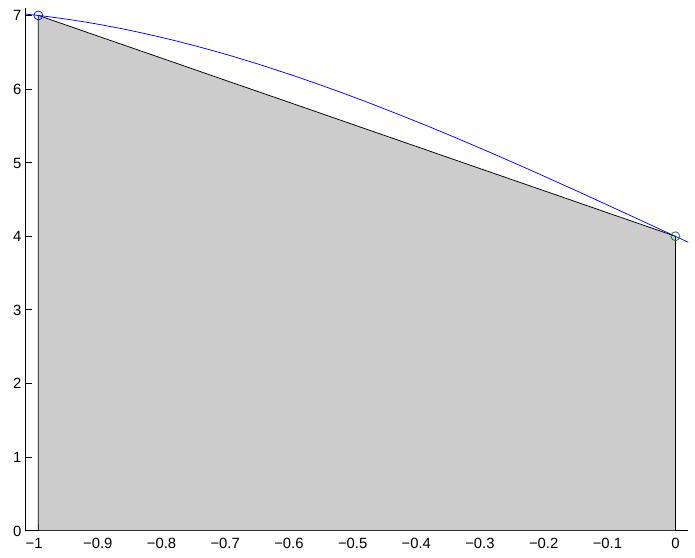
\includegraphics[width=\textwidth]{2025_09_05_3888c9ac96bd653d96b4g-139}
\captionsetup{labelformat=empty}
\caption{Figura 7.1. Regla de los Trapecios simple cerrada}
\end{center}
\end{figure}

La recta está dada por $p(x)=f(a)+\frac{f(b)-f(a)}{b-a}(x-a)$, integrado $p$ obtenemos

$$
\begin{aligned}
\int_{a}^{b} p(x) d x & =f(a) x+\left.\frac{f(b)-f(a)}{b-a} \frac{(x-a)^{2}}{2}\right|_{a} ^{b} \\
& =f(a)(b-a)+\frac{f(b)-f(a)}{2}(b-a)
\end{aligned}
$$

es decir:


\begin{equation*}
\int_{a}^{b} f(x) d x \quad \sim \quad T(f)=\frac{(b-a)}{2}(f(a)+f(b)) \tag{7.2}
\end{equation*}


Ejemplo 7.1. Consideremos la función $f(x)=x^{3}-4 x+4$ en el intervalo $[-1,0]$. ¿Cuál es el valor aproximado de la integral en este intervalo que da la regla de trapecios?

Según vimos, se tiene

$$
\int_{-1}^{0} x^{3}-4 x+4 d x \sim \frac{0-(-1)}{2}(f(-1)+f(0))=\frac{1}{2}(7+4)=\frac{11}{2}
$$

En este caso, es sencillo calcular el valor exacto de $\int_{-1}^{0} x^{3}-4 x+4 d x=\frac{23}{4}$ con lo cual se puede calcular exactamente el error que se comete, $R(f)=\frac{1}{4}=0,25$.

Más adelante nos dedicaremos al estudio del error. Veamos ahora una pequeña modificación a la regla de trapecios.

Regla de Trapecios abierta: en este caso, en lugar de considerar como nodos los extremos del intervalo $[a, b]$ vamos a usar dos puntos interiores equiespaciados $\left\{x_{1}, x_{2}\right\}$. Luego, sustituímos la función $f$ por la recta que la interpola en esos nodos (ver Figura 7.2). Para ésto partimos al intervalo $[a, b]$ en tercios, es decir en subintervalos de longitud $h=\frac{b-a}{3}$. De esta manera consideramos $\left\{x_{1}, x_{2}\right\}$ los extremos del intervalo medio, es decir $x_{j}=a+j h$ para $j=1,2$. El polinomio de grado 1 que interpola a $f$ en esos nodos es

$$
p(x)=f\left(x_{1}\right)+\frac{f\left(x_{2}\right)-f\left(x_{1}\right)}{x_{2}-x_{1}}\left(x-x_{1}\right) .
$$

Integrando $p$ en $[a, b]$ y recordando que $h=\frac{b-a}{3}$ (ésto es: $b-a=3 h, x_{2}-x_{1}=h, b-x_{1}=2 h$, y $\left.a-x_{1}=-h\right)$ tenemos

\begin{figure}[h]
\begin{center}
  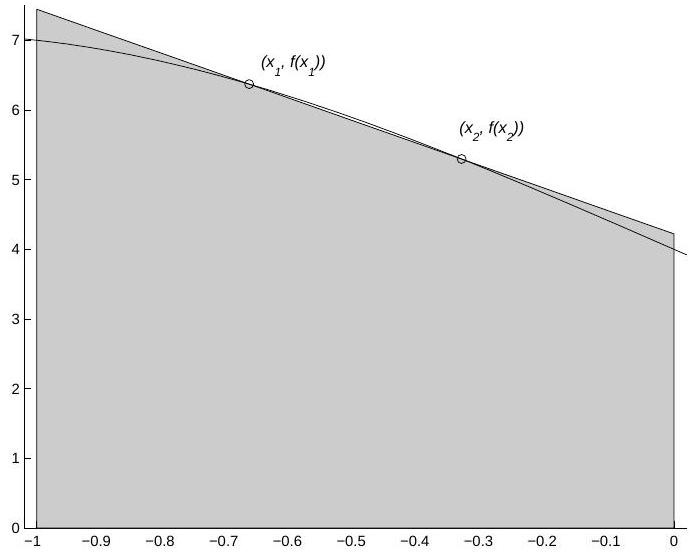
\includegraphics[width=\textwidth]{2025_09_05_3888c9ac96bd653d96b4g-140}
\captionsetup{labelformat=empty}
\caption{Figura 7.2. Regla de Trapecios simple abierta}
\end{center}
\end{figure}

$$
\begin{aligned}
\int_{a}^{b} p(x) d x & =f\left(x_{1}\right) x+\left.\frac{f\left(x_{2}\right)-f\left(x_{1}\right)}{x_{2}-x_{1}} \frac{\left(x-x_{1}\right)^{2}}{2}\right|_{a} ^{b} \\
& =f\left(x_{1}\right) 3 h+\frac{f\left(x_{1}\right)-f\left(x_{2}\right)}{h}\left[\frac{(2 h)^{2}-(-h)^{2}}{2}\right] \\
& =3 h f\left(x_{1}\right)+\frac{f\left(x_{1}\right)-f\left(x_{2}\right)}{h} \frac{3 h^{2}}{2} \\
& =3 h\left(\frac{f\left(x_{1}\right)+f\left(x_{2}\right)}{2}\right)
\end{aligned}
$$

Luego, para $h=\frac{b-a}{3}$,


\begin{equation*}
\int_{a}^{b} f(x) d x \quad \sim \quad \frac{3 h}{2}\left(f\left(x_{1}\right)+f\left(x_{2}\right)\right) \tag{7.3}
\end{equation*}


Ejemplo 7.2. Consideremos nuevamente la función $f(x)=x^{3}-4 x+4$ en el intervalo $[-1,0]$. Queremos calcular la aproximación que da la fórmula de Trapecios abierta.

La regla de trapecios abierta tienen por nodos $\left\{x_{1}=-\frac{2}{3}, x_{2}=-\frac{1}{3}\right\}$ con $h=\frac{1}{3}$. El valor aproximado de la integral de $f$ en $[-1,0]$ es\\
$\int_{-1}^{0} x^{3}-4 x+4 d x \sim \frac{1}{2}\left(f\left(-\frac{2}{3}\right)+f\left(-\frac{1}{3}\right)\right)=\frac{1}{2}\left(-\frac{8}{27}+\frac{8}{3}+4-\frac{1}{27}+\frac{4}{3}+4\right)=\frac{1}{2} \frac{53}{3}=5,8333 \ldots$

Usando el valor exacto, ya calculado, de $\int_{-1}^{0} x^{3}-4 x+4 d x=\frac{23}{4}$ podemos asegurar que el error cometido es, $R(f)=-0,08333 \ldots$

Regla de Simpson: es la que se obtiene si se reemplaza en el intervalo $[a, b]$ la integral de la función $f$ por la de una función cuadrática que interpola a $f$. Como para dar un único polinomio de grado 2 que interpole a $f$ se necesitan tres nodos, se consideran los extremos del intervalo y su punto medio, es decir, $\left\{a, \frac{a+b}{2}, b\right\}$ (ver Figura 7.3). Como $a$ y $b$ forman parte de los nodos, esta fórmula también suele llamarse de Simpson cerrada.

\begin{figure}[h]
\begin{center}
  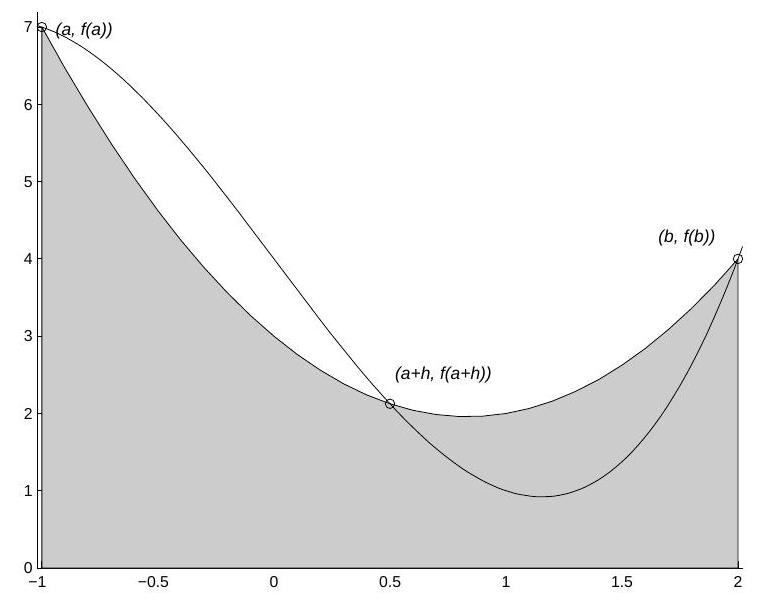
\includegraphics[width=\textwidth]{2025_09_05_3888c9ac96bd653d96b4g-141}
\captionsetup{labelformat=empty}
\caption{Figura 7.3. Regla de Simpson}
\end{center}
\end{figure}

Para simplificar los cálculos, queremos hallar la fórmula que le corresponde a una función continua cuando se considera el intervalo $[-1,1]$ y derivar de ésta la fórmula general. Para ésto necesitaremos el siguiente lema.

Lema 7.3. Si $Q_{0}(f)=\sum_{j=0}^{n} A_{j} f\left(t_{j}\right)$ es una fórmula de cuadratura para aproximar la integral $\int_{-1}^{1} f(x) d x$ entonces, para

$$
x_{j}=\frac{(b-a)}{2} t_{j}+\frac{(a+b)}{2}, \quad \forall j=0, \ldots, n ;
$$

se tiene una fórmula de cuadratura para el intervalo $[a, b]$ :


\begin{equation*}
\int_{a}^{b} f(x) d x \quad \sim \quad Q(f)=\sum_{j=0}^{n} \frac{(b-a)}{2} A_{j} f\left(x_{j}\right) \tag{7.4}
\end{equation*}


Demostración. Consideremos el cambio de variables $x=\alpha t+\beta$, con $\alpha=(b-a) / 2$ y $\beta=(a+b) / 2$ que transforma el intervalo $[-1,1]$ en $[a, b]$. Así,

$$
\int_{a}^{b} f(x) d x=\int_{-1}^{1} f(\alpha t+\beta) \alpha d t
$$

Aplicando la fórmula $Q_{0}$ a la función $g(t)=\alpha f(\alpha t+\beta)$ para el intervalo $[-1,1]$ tenemos,


\begin{equation*}
\int_{a}^{b} f(x) d x=\int_{-1}^{1} f(\alpha t+\beta) \alpha d t \quad \sim \quad Q_{0}(g) \tag{7.5}
\end{equation*}


con,

$$
Q_{0}(g)=\sum_{j=0}^{n} A_{j} g\left(t_{j}\right)=\sum_{j=0}^{n} \alpha A_{j} f\left(\alpha t_{j}+\beta\right) .
$$

Si llamamos $x_{j}=\alpha t_{j}+\beta$, para $j=0, \ldots, n$, tenemos que

$$
x_{j}=\frac{(b-a)}{2} t_{j}+\frac{(a+b)}{2} \quad \forall j=0, \ldots, n .
$$

Luego, podemos re-escribir la aproximación en $[a, b]$ dada en (7.5) como en la fórmula (7.4).

Ahora sí, procedemos a dar la fórmula de Simpson, que aproxima a $\int_{-1}^{1} f(x) d x$, usando el polinomio interpolador $p$ en los nodos equiespaciados $\{-1,0,1\}$. Si $p(x)=a_{0}+a_{1} x+a_{2} x^{2}$,

$$
\int_{-1}^{1} p(x) d x=2\left[a_{0}+\frac{a_{2}}{3}\right]=\frac{2}{6}\left[6 a_{0}+2 a_{2}\right] .
$$

Por otro lado, sabemos que $p(x)=a_{0}+a_{1} x+a_{2} x^{2}$ verifica el sistema:

$$
\left(\begin{array}{ccc}
1 & -1 & 1 \\
1 & 0 & 0 \\
1 & 1 & 1
\end{array}\right)\left(\begin{array}{l}
a_{0} \\
a_{1} \\
a_{2}
\end{array}\right)=\left(\begin{array}{c}
f(-1) \\
f(0) \\
f(1)
\end{array}\right)
$$

Por lo tanto, $a_{0}=f(0), a_{1}=\frac{f(1)-f(-1)}{2}$ y $a_{2}=\frac{f(-1)-2 f(0)+f(1)}{2}$.\\
Luego,

$$
\int_{-1}^{1} f(x) d x \quad \sim \quad \int_{-1}^{1} p(x) d x=\frac{2}{6}[f(-1)+4 f(0)+f(1)]
$$

Ahora, por el Lema 7.3, se tiene para un intervalo $[a, b]$ la fórmula de Simpson simple cerrada:

$$
S(f)=\frac{(b-a)}{6}[f(a)+4 f((a+b) / 2)+f(b)]
$$

Si escribimos la fórmula en términos de la distancia entre un nodo y otro, $h=\frac{b-a}{2}$, se tiene:


\begin{equation*}
S(f)=\frac{h}{3}[f(a)+4 f(a+h)+f(b)] \tag{7.6}
\end{equation*}


Ejemplo 7.4. Para la función $f(x)=x^{3}-4 x+4$ consideremos ahora el intervalo $[-1,2]$. ¿Cuál es el valor que se obtiene al aproximar la integral de $f$ en este intervalo si se emplea la fórmula de Simpson cerrada?

Para este intervalo tenemos, $b-a=3$, luego $h=\frac{3}{2}$ y $a+h=\frac{a+b}{2}=\frac{1}{2}$, entonces la fómula (7.6) nos da

$$
S(f)=\frac{1}{2}\left[f(-1)+4 f\left(\frac{1}{2}\right)+f(2)\right]=\frac{1}{2}\left[7+4 \frac{17}{8}+4\right]=\frac{39}{4}
$$

En este caso el cálculo es exacto puesto que al calcular la integral de $f$ en $[-1,2]$ obtenemos por resultado $\frac{39}{4}$.

Regla de Simpson abierta: es la que se obtiene al reemplazar $f$ por un polinomio de grado 2 que la interpola en nodos equiespaciados en el interior del intervalo $[a, b]$. Para ésto partimos al intervalo $[a, b]$ en cuartos, es decir en subintervalos de longitud $h=\frac{b-a}{4}$. De esta manera consideramos $\left\{x_{1}, x_{2}, x_{3}\right\}$ los extremos de los intervalos medios, es decir $x_{j}=a+j h$ para $j=1,2,3$; (ver Figura 7.4). Como $a$ y $b$ no forman parte de los nodos, esta fórmula recibe el nombre de Simpson abierta.

Si procedemos como antes, podemos hallar el polinomio de grado 2 que interpola a una función en el intervalo $[-1,1]$ y luego por el Lema 7.3 extendemos la fórmula a cualquier intervalo $[a, b]$. En este caso, el polinomio $p(x)=a_{0}+a_{1} x+a_{2} x^{2}$ interpola a $f$ en los nodos $\left\{-\frac{1}{2}, 0, \frac{1}{2}\right\}$. y resultan $a_{0}=f(0), a_{1}=f\left(\frac{1}{2}\right)-f\left(-\frac{1}{2}\right)$, y $a_{2}=2 f\left(-\frac{1}{2}\right)-4 f(0)+2 f\left(\frac{1}{2}\right)$.

\begin{figure}[h]
\begin{center}
  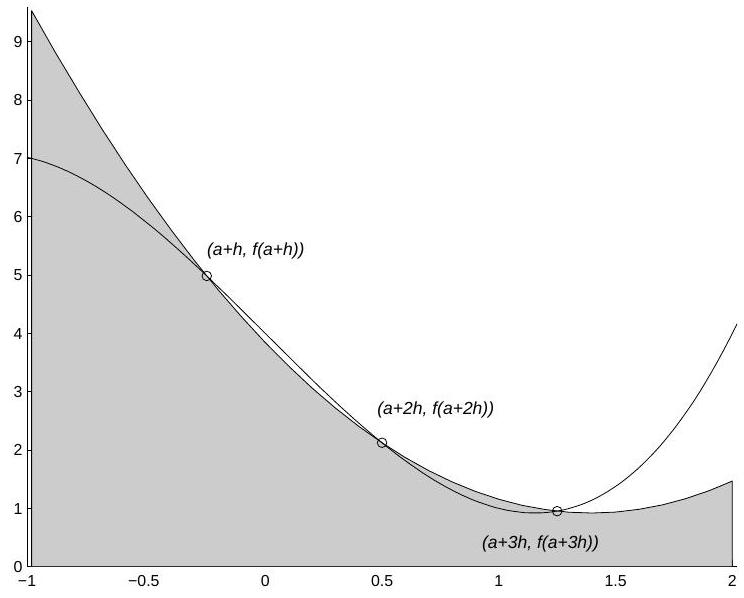
\includegraphics[width=\textwidth]{2025_09_05_3888c9ac96bd653d96b4g-144}
\captionsetup{labelformat=empty}
\caption{Figura 7.4. Regla de Simpson abierta}
\end{center}
\end{figure}

Luego, $\int_{-1}^{1} p(x) d x=\frac{2}{3}\left[3 a_{0}+a_{2}\right]=\frac{2}{3}\left[2 f\left(-\frac{1}{2}\right)-f(0)+2 f\left(\frac{1}{2}\right)\right]$. Al pasar a un intervalo $[a, b]$ por medio del Lema 7.3 y escribiendo la fórmula en términos del paso $h=\frac{b-a}{4}$ obtenemos,

$$
\int_{a}^{b} f(x) d x \quad \sim \quad \frac{4 h}{3}[2 f(a+h)-f(a+2 h)+2 f(a+3 h)]
$$

Ejemplo 7.5. Consideremos nuevamente la función $f(x)=x^{3}-4 x+4$ en el intervalo $[-1,2]$. Queremos hallar una aproximación de la integral de $f$ en dicho intervalo por medio de la regla de Simpson abierta.

Como $h=\frac{b-a}{4}=\frac{3}{4}$, entonces $a+h=-\frac{1}{4}, a+2 h=\frac{1}{2}, a+3 h=\frac{5}{4}$, así tenemos

$$
\int_{-1}^{2} x^{3}-4 x+4 d x \quad \sim 1\left[2 f\left(-\frac{1}{4}\right)-f\left(\frac{1}{2}\right)+2 f\left(\frac{5}{4}\right)\right]=\left[2 \frac{319}{64}-\frac{17}{8}+2 \frac{61}{64}\right]=\frac{624}{64}=\frac{39}{4},
$$

que vuelve a ser un cálculo exacto.

Es claro que la fórmula de Simpson es exacta para polinomios de $\mathcal{P}_{2}$ y que la fórmula de Trapecios lo es para polinomios de $\mathcal{P}_{1}$. En general, una regla como la dada en (7.1), construida interpolando en $n+1$ puntos, es exacta para polinomios de $\mathcal{P}_{n}$, sin embargo, veremos que para ciertas elecciones de puntos la regla resulta exacta también para polinomios de $\mathcal{P}_{k}$ para algún $k>n$. Por otra parte, veremos luego que el grado de polinomios para el cual una regla es exacta se relaciona con el error cometido al usar dicha regla. Esto motiva la siguiente definición.

Definición 7.6. Decimos que una fórmula de cuadratura $Q(f)=\sum_{j=0}^{n} A_{j} f\left(x_{j}\right)$ tiene grado de exactitud $k$, si $\int_{a}^{b} p(x) d x=Q(p)$ para todo polinomio $p \in \mathcal{P}_{k}$ y no para $\mathcal{P}_{k+1}$.

ObSERVACIÓN 7.7. Toda fórmula de cuadratura $\int_{a}^{b} f(x) d x \quad \sim \quad Q(f)=\sum_{j=0}^{n} A_{j} f\left(x_{j}\right)$ es lineal. Es decir, $Q(\alpha f+g)=\alpha Q(f)+Q(g)$ para todo $\alpha \in \mathbb{R}, f$ y $g$ funciones.

En virtud de este resultado, podemos reducir el estudio del grado de exactitud al comportamiento de la fórmula sobre una base del espacio de polinomios. Esto queda expresado en la siguiente observación.

Observación 7.8. Una fórmula de cuadratura $Q$ tiene grado de exactitud $k$ si y solo si es exacta para la base de $\mathcal{P}_{k}, \mathcal{B}=\left\{1, x, x^{2}, \ldots, x^{k}\right\}$ y no lo es para el polinomio $x^{k+1}$. Esto es, la igualdad

$$
\int_{a}^{b} x^{m} d x=\sum_{j=0}^{n} A_{j} x_{j}^{m}
$$

debe verificarse para todo $m=0, \ldots, k$ y no para $m=k+1$.\\
Además, gracias al Lema 7.3, una fórmula de cuadratura tiene grado de exactitud $k$ independientemente del intervalo $[a, b]$ para el cual está calculada.

Ejemplo 7.9. Se quiere calcular el grado de exactitud de la fórmula de Simpson cerrada.

Es claro que las fórmulas de Simpson, tanto abiertas como cerradas, son exactas para polinomios de $\mathcal{P}_{2}$. Luego, por Observación 7.8, basta ver qué sucede con $x^{3}, x^{4}, \ldots$, y esto puede hacerse, sin perder generalidad, en el intervalo $[-1,1]$. Tenemos

$$
\begin{aligned}
\int_{-1}^{1} x^{3} d x & =0=\frac{2}{6}\left[(-1)^{3}+4(0)^{3}+(1)^{3}\right] \\
\int_{-1}^{1} x^{4} d x & =\frac{2}{5} \neq \frac{2}{3}=\frac{1}{3}\left[(-1)^{4}+4(0)^{4}+(1)^{4}\right]
\end{aligned}
$$

Luego, la fórmula de Simpson cerrada tiene grado de exactitud $k=3$. Lo mismo sucederá para la fórmula abierta.

\section{Estimación del error}
En lo que sigue notaremos por $I(f)=\int_{a}^{b} f(x) d x$. Una vez obtenida una regla de cuadratura $Q(f)$ surge la pregunta de qué se puede decir sobre el error cometido $R(f)=I(f)-Q(f)$.

La forma más usual de aproximar integrales es mediante las llamadas reglas de integración compuestas que veremos más adelante, las cuales se basan en partir el intervalo $[a, b]$ en intervalos chicos y aplicar en cada uno de ellos alguna de las reglas construídas mediante interpolación. Por esta razón nos interesa saber como es el error en términos de la longitud del intervalo donde se aplica la regla. El siguiente teorema nos da un resultado general que nos dice que el error depende del grado de exactitud de la regla.

Teorema 7.10. Dada una regla de cuadratura $Q(f)$ en el intervalo $[a, b]$ tal que\\
i) $Q(f)$ es lineal,\\
ii) $Q(f)$ tiene grado de exactitud $k$,\\
iii) $|Q(f)| \leq M(b-a)\|f\|_{\infty}$, para alguna constante $M$.

Entonces, si $f \in C^{k+1}[a, b]$, se tiene

$$
|R(f)|=|I(f)-Q(f)| \leq \frac{(1+M)(b-a)^{k+2}}{(k+1)!}\left\|f^{k+1}\right\|_{\infty}
$$

Demostración. Observemos que, como $f \in C^{k+1}[a, b]$, existe un polinomio $p_{k} \in \mathcal{P}_{k}$ tal que

$$
\left\|f-p_{k}\right\|_{\infty} \leq \frac{(b-a)^{k+1}}{(k+1)!}\left\|f^{k+1}\right\|_{\infty}
$$

En efecto, podemos tomar por ejemplo el polinomio dado por el desarrollo de Taylor de $f$ en cualquier punto del intervalo.

Entonces, como la regla tiene exactitud $k$, tenemos que $I\left(p_{k}\right)=Q\left(p_{k}\right)$. Luego, usando la linealidad de $Q(f)$,

$$
R(f)=I(f)-Q(f)=I\left(f-p_{k}\right)-Q\left(f-p_{k}\right)
$$

Por lo tanto, usando la hipótesis $i i i)$ y que $\left|I\left(f-p_{k}\right)\right| \leq(b-a)\left\|f-p_{k}\right\|_{\infty}$, obtenemos

$$
|R(f)| \leq\left|I\left(f-p_{k}\right)\right|+\left|Q\left(f-p_{k}\right)\right| \leq \frac{(1+M)(b-a)^{k+2}}{(k+1)!}\left\|f^{k+1}\right\|_{\infty}
$$

concluyendo la demostración.

Observación 7.11. Si la regla está dada como en (7.1) con $A_{j}>0$ para todo $j=0, \ldots, n$, y tiene grado de exactitud al menos 0 , entonces la hipótesis $i i i)$ del teorema se cumple con $M=1$. En efecto, como la regla es exacta para constantes se tiene que $\sum_{j=0}^{n} A_{j}=Q(1)=I(1)=(b-a)$ y por lo tanto,

$$
|Q(f)|=\left|\sum_{j=0}^{n} A_{j} f\left(x_{j}\right)\right| \leq \sum_{j=0}^{n} A_{j}\left|f\left(x_{j}\right)\right| \leq(b-a)\|f\|_{\infty}
$$

Consideremos la regla del trapecio en el intervalo $[a, b]$. Como ésta tiene grado de exactitud 1 el Teorema 7.10 y la Observación 7.11 nos dicen que

$$
|I(f)-T(f)| \leq(b-a)^{3}\left\|f^{(3)}\right\|_{\infty}
$$

Tomando por ejemplo la función $f(x)=(x-a)^{2}$ y calculando $I(f)$ y $T(f)$ observamos que

$$
I(f)-T(f)=-\frac{(b-a)^{3}}{6}
$$

lo que muestra que el orden obtenido en términos de la longitud del intervalo no puede mejorarse.\\
Lo que sí se puede es, analizando cada regla en particular, obtener una expresión más precisa del error mejorando en particular la constante que aparece en la estimación de éste. Esto es lo que haremos a continuación para algunas de las reglas clásicas. Para esto necesitamos la siguiente versión del teorema del valor medio para integrales, la cual es un poco más general que la que se ve en los cursos elementales de Cálculo.

Teorema 7.12. (Valor Medio Integral Generalizado). Si $g:[a, b] \rightarrow \mathbb{R}, \xi:[a, b] \rightarrow[c, d]$, $y h:[c, d] \rightarrow \mathbb{R}$ son tales que $g$ es continua y no cambia de signo, $h$ es continua y $h(\xi(x)) g(x)$ es una función integrable, entonces existe $\eta \in(c, d)$ tal que

$$
\int_{a}^{b} h(\xi(x)) g(x) d x=h(\eta) \int_{a}^{b} g(x) d x
$$

Demostración. Supongamos que $g(x) \geq 0$ (el caso $g(x) \leq 0$ se hace de manera análoga). Sean $m$ y $M$ el mínimo y máximo de $h$ respectivamente. Entonces, $m \leq h(\xi(x)) \leq M$ y por lo tanto $m g(x) \leq h(\xi(x)) g(x) \leq M g(x)$ para todo $x \in[a, b]$. Integrando obtenemos,

$$
m \int_{a}^{b} g(x) d x \leq \int_{a}^{b} h(\xi(x)) g(x) d x \leq M \int_{a}^{b} g(x) d x
$$

y como $\int_{a}^{b} g(x) d x>0$ (suponiendo que $g$ no es idénticamente cero) resulta,

$$
m \leq \frac{\int_{a}^{b} h(\xi(x)) g(x) d x}{\int_{a}^{b} g(x) d x} \leq M
$$

y por lo tanto, como $h$ es continua, por el teorema de Bolzano sabemos que existe $\eta \in(c, d)$ tal que

$$
h(\eta)=\frac{\int_{a}^{b} h(\xi(x)) g(x) d x}{\int_{a}^{b} g(x) d x}
$$

lo que concluye la demostración.

El otro ingrediente para obtener las fórmulas del error para las reglas de cuadratura es la expresión para el error de interpolación estudiada en el capítulo anterior. El Teorema 5.4 nos dice que, para cualquier función $f \in C^{n+1}[a, b]$, si $p_{n} \in \mathcal{P}_{n}$ es su polinomio interpolador se tiene

$$
E_{n}(x)=f(x)-p_{n}(x)=\frac{f^{(n+1)}(\xi)}{(n+1)!} W_{n+1}(x) \quad \text { con } \xi \in(a, b) \text { que depende de } x .
$$

Luego, si $Q$ es una fórmula de cuadratura como en (7.1) podemos expresar el error de integración como

$$
R(f)=I(f)-Q(f)=\int_{a}^{b}\left(f-p_{n}\right)(x) d x
$$

Es decir

$$
R(f)=\int_{a}^{b} \frac{f^{(n+1)}(\xi)}{(n+1)!} W_{n+1}(x) d x
$$

Teorema 7.13. (Error para la Regla de Trapecios) Si $f \in C^{2}[a, b]$, el error que se produce al aproximar $\int_{a}^{b} f(x) d x$ usando la regla de Trapecios está dado por


\begin{equation*}
R(f)=-\frac{(b-a)^{3}}{12} f^{\prime \prime}(\eta), \quad \text { para algún } \eta \in(a, b) . \tag{7.7}
\end{equation*}


Demostración. Para calcular el error de la regla de los trapecios recordemos que los nodos son $\{a, b\}$, y por tanto $W_{2}(x)=(x-a)(x-b)$, que no cambia de signo en $[a, b]$, entonces usando el Teorema 7.12,

$$
\begin{aligned}
R(f) & =I(f)-Q(f)=\int_{a}^{b} \frac{f^{\prime \prime}(\xi)}{2!} W_{2}(x) d x \\
& =\frac{f^{\prime \prime}(\eta)}{2} \int_{a}^{b}(x-a)(x-b) d x \\
& =-\frac{f^{\prime \prime}(\eta)}{12}(b-a)^{3}
\end{aligned}
$$

Notar que hay una forma directa de calcular $\int_{a}^{b}(x-a)(x-b) d x$ que es calcularla por partes. Si derivamos $(x-b)$ e integramos $(x-a)$, tenemos

$$
\int_{a}^{b}(x-a)(x-b) d x=\left.(x-b) \frac{(x-a)^{2}}{2}\right|_{a} ^{b}-\int_{a}^{b} \frac{(x-a)^{2}}{2} d x=-\left.\frac{(x-a)^{3}}{6}\right|_{a} ^{b}=-\frac{(b-a)^{3}}{6} .
$$

Ejemplo 7.14. Estimar el error cometido al aproximar $\int_{0}^{\frac{1}{2}} x^{4}-x^{2}+2 x+3 d x$ por la fórmula de trapecios cerrada. ¿Cuál es el valor de dicha aproximación? ¿Qué análisis se puede hacer si se considera la misma función en el intervalo $[-1,1]$ ?

Si $h=b-a$ tenemos $h=\frac{1}{2}, f(x)=x^{4}-x^{2}+2 x+3$ y $f^{\prime \prime}(x)=12 x^{2}-2$. Como $R(f)=-\frac{h^{3}}{12} f^{\prime \prime}(\eta)$ para algún $\eta \in\left(0, \frac{1}{2}\right)$, acotamos $\left|f^{\prime \prime}(x)\right|$ para todo $x \in\left[0, \frac{1}{2}\right]$. Esto es, $\left|f^{\prime \prime}(x)\right| \leq 2$, puesto que alcanza su valor máximo en el extremo izquierdo del intervalo.

Luego, $|R(f)|=\frac{h^{3}}{12}\left|f^{\prime \prime}(\eta)\right| \leq \frac{1}{8} \frac{1}{12} 2=0,020833 \ldots$\\
El valor de la aproximación está dado por $T(f)=\frac{1}{4}\left(f(0)+f\left(\frac{1}{2}\right)\right)=\frac{1}{4}\left(3+\frac{61}{16}\right)=3,81250$\\
A veces, al estimar el error perdemos información. Por ejemplo, si queremos estimar el error cometido al considerar $x \in[-1,1]$, no logramos un resultado muy fino. Por un lado $\left|f^{\prime \prime}(x)\right|= \left|12 x^{2}-2\right| \leq 10$, pues alcanza su valor máximo en los extremos del intervalo y $h=b-a=2$, así,\\
$|R(f)|=\frac{h^{3}}{12}\left|f^{\prime \prime}(\eta)\right| \leq \frac{8}{12} 10=\frac{20}{3}=6,666 \ldots$\\
Aunque $\int_{-1}^{1} x^{4}-x^{2}+2 x+3 d x=\frac{86}{15}=5,7333 \ldots$ y el valor que arroja la fórmula es $T(f)= \frac{2}{2}(f(-1)+f(1))=6 \mathrm{y}$ el error real es $0,2666 \ldots$

Analizar el error para la regla de Simpson es un poco más difícil pues el polinomio $W_{3}(x)= (x-a)\left(x-\frac{a+b}{2}\right)(x-b)$ cambia de signo en $[a, b]$ y por lo tanto no se puede aplicar directamente un argumento análogo al usado para la regla de Trapecios. Hay varias formas de obtener la fórmula del error para la regla de Simpson. Daremos aquí la que consideramos más elemental pues utiliza sólo herramientas de los cursos básicos de Cálculo.

Teorema 7.15. (Error para la Regla de Simpson) Si $f \in C^{4}[a, b]$, el error que se produce al aproximar $\int_{a}^{b} f(x) d x$ usando la regla de Simpson está dado por


\begin{equation*}
R(f)=-\frac{1}{90}\left(\frac{b-a}{2}\right)^{5} f^{(4)}(\eta), \quad \text { para algún } \eta \in(a, b) . \tag{7.8}
\end{equation*}


Demostración. Consideremos el intervalo $[-h, h]$. Definamos

$$
F(x)=\int_{0}^{x} f(x) d x
$$

y, para $t \in[-h, h]$,

$$
e(t)=F(t)-F(-t)-t\left[\frac{1}{3} f(-t)+\frac{1}{3} f(0)+\frac{4}{3} f(t)\right]
$$

de tal forma que

$$
R(f)=I(f)-S(f)=e(h)
$$

Nuestro objetivo es entonces encontrar una expresión para $e(h)$. Derivando obtenemos,

$$
\begin{gathered}
e^{\prime}(t)=\frac{2}{3} f(t)+\frac{2}{3} f(-t)-\frac{4}{3} f(0)+\frac{t}{3} f^{\prime}(-t)-\frac{t}{3} f^{\prime}(t) \\
e^{\prime \prime}(t)=\frac{1}{3} f^{\prime}(t)-\frac{1}{3} f^{\prime}(-t)-\frac{t}{3} f^{\prime \prime}(-t)-\frac{t}{3} f^{\prime \prime}(h)
\end{gathered}
$$

y

$$
e^{(3)}(t)=\frac{t}{3}\left[f^{(3)}(-t)-f^{(3)}(t)\right]
$$

Entonces, por el teorema del valor medio, existe $\xi_{1}=\xi_{1}(t)$ tal que

$$
e^{(3)}(t)=-\frac{2}{3} t^{2} f^{(4)}\left(\xi_{1}\right)
$$

Observemos que $e(0)=0$ y que de las expresiones obtenidas resulta que también $e^{\prime}(0)=e^{\prime \prime}(0)=$ 0 . Por lo tanto, integrando entre 0 y $h$ y usando el Teorema 7.12, obtenemos

$$
e^{\prime \prime}(h)=\int_{0}^{h} e^{(3)}(t) d t=-\frac{2}{3} \int_{0}^{h} t^{2} f^{(4)}\left(\xi_{1}\right) d t=-\frac{2}{3} f^{(4)}\left(\xi_{2}\right) \int_{0}^{h} t^{2} d t=-\frac{2}{9} f^{(4)}\left(\xi_{2}\right) h^{3}
$$

para algún $\xi_{2}=\xi_{2}(h)$. Análogamente, existe un $\xi_{3}=\xi_{3}(h)$ tal que,

$$
e^{\prime}(h)=\int_{0}^{h} e^{\prime \prime}(t) d t=-\frac{2}{36} f^{(4)}\left(\xi_{3}\right) h^{4}
$$

e integrando una vez más, obtenemos que existe un $\eta \in[-h, h]$ tal que

$$
e(h)=-\frac{h^{5}}{90} f^{(4)}(\eta)
$$

Ahora, en cualquier intervalo $[a, b]$, mediante un cambio de variable, se obtiene

$$
R(f)=-\frac{1}{90}\left(\frac{b-a}{2}\right)^{5} f^{(4)}(\eta)
$$

para algún punto intermedio $\eta \in(a, b)$; como queríamos demostrar.

Ejemplo 7.16. Aproximar $\int_{0}^{1} e^{-x^{2}} d x$ mediante la regla de Simpson cerrada y estimar el error que se comete al efectuar dicho cálculo.

Tenemos $h=\frac{1}{2}, f(x)=e^{-x^{2}}$, así\\
$\int_{0}^{1} e^{-x^{2}} d x \sim \frac{1}{6}\left(f(0)+4 f\left(\frac{1}{2}\right)+f(1)\right)=\frac{1}{6}\left(1+e^{-\frac{1}{4}}+e^{-1}\right)=0,74951 \ldots$\\
Para estimar el error consideramos $f^{i v}(x)=4\left(4 x^{4}-12 x^{2}+3\right) e^{-x^{2}}$. Como $R(f)=\frac{-h^{5}}{90} f^{(i v)}(\eta)$ para algún $\eta \in(0,1)$, acotamos $\left|f^{\prime \prime}(x)\right|$ para todo $x \in[0,1]$.

Por una parte tenemos que en $[0,1], e^{-x^{2}} \leq 1$ y por otra parte puede verse que $\left|4 x^{4}-12 x^{2}+3\right|$ alcanza su valor máximo en el extremo superior del intervalo. Luego, $\left|4 x^{4}-12 x^{2}+3\right| \leq 5$ en $[0,1]$ y por lo tanto

$$
|R(f)| \leq \frac{1}{90}\left(\frac{1}{2}\right)^{5} 20=0,006944 \ldots
$$

\section{Fórmulas de cuadratura compuestas}
Si queremos aumentar la precisión al aproximar $\int_{a}^{b} f(x) d x$, podemos aumentar el número de nodos. Esto es, considerar $n+1$ nodos y el polinomio de $\mathcal{P}_{n}$ que interpola a $f$ en esos nodos, con $n \in \mathbb{N}$ grande. Esto no siempre es conducente. Como vimos en el Capítulo 5, aumentar el grado del polinomio interpolador puede producir errores grandes en la aproximación, los que podrían trasladarse al cálculo de la integral. Otra posibilidad es partir el intervalo $[a, b]$ en pequeños subintervalos y en cada uno de estos aplicar una aproximación del tipo Trapecios o Simpson. Este método que vamos a desarrollar en esta sección es el más usual y se conoce como "cuadratura compuesta".

La idea general es como sigue. Partimos el intervalo $[a, b]$ en subintervalos eligiendo puntos $x_{j}$ con $a=x_{0}<x_{1}<\ldots<x_{n}=b$. Sabemos que

$$
I(f)=\int_{a}^{b} f(x) d x=\sum_{j=0}^{n-1} \int_{x_{j}}^{x_{j+1}} f(x) d x
$$

Ahora si para cada

$$
I_{j}(f)=\int_{x_{j}}^{x_{j+1}} f(x) d x
$$

tenemos una fórmula de cuadratura $Q_{j}(f)$ y consideramos el error respectivo,

$$
R_{j}(f)=I_{j}(f)-Q_{j}(f)
$$

obtenemos

$$
\begin{aligned}
R(f)=\sum_{j=0}^{n-1} R_{j}(f) & =\sum_{j=0}^{n-1}\left(I_{j}(f)-Q_{j}(f)\right) \\
& =\int_{a}^{b} f(x) d x-\sum_{j=0}^{n-1} Q_{j}(f)
\end{aligned}
$$

Esto es, la fórmula de cuadratura será


\begin{equation*}
\int_{a}^{b} f(x) d x \sim \sum_{j=0}^{n-1} Q_{j}(f) \quad \text { con error } \quad R(f)=\sum_{j=0}^{n-1} R_{j}(f) \tag{7.9}
\end{equation*}


Usando el Teorema 7.10 podemos obtener un resultado general de estimación del error.\\
Teorema 7.17. Sea $Q(f)$ una regla de cuadratura como en (7.9) donde cada $Q_{j}(f)$ es lineal, tiene grado de exactitud $k$ y satisface en el intervalo $\left[x_{j}, x_{j+1}\right]$ que $\left|Q_{j}(f)\right| \leq M\left(x_{j+1}-x_{j}\right)\|f\|_{\infty}$, para alguna constante $M$.

Entonces, si $f \in C^{k+1}[a, b]$ y $h=\operatorname{máx}_{j}\left(x_{j+1}-x_{j}\right)$ se tiene que

$$
|R(f)|=|I(f)-Q(f)| \leq \frac{(1+M)(b-a)}{(k+1)!} h^{k+1}\left\|f^{k+1}\right\|_{\infty} .
$$

Demostración. Por el Teorema 7.10 sabemos que

$$
\left|R_{j}(f)\right| \leq \frac{(1+M)\left(x_{j+1}-x_{j}\right)^{k+2}}{(k+1)!}\left\|f^{k+1}\right\|_{\infty}
$$

En consecuencia, acotando $\left(x_{j+1}-x_{j}\right)^{k+1}$ por $h^{k+1}$ se tiene

$$
\begin{aligned}
|R(f)| \leq & \sum_{j=0}^{n-1}\left|R_{j}(f)\right| \leq \frac{(1+M)}{(k+1)!} \sum_{j=0}^{n-1}\left(x_{j+1}-x_{j}\right)^{k+2}\left\|f^{k+1}\right\|_{\infty} \\
& \leq \frac{(1+M)}{(k+1)!} \sum_{j=0}^{n-1}\left(x_{j+1}-x_{j}\right) h^{k+1}\left\|f^{k+1}\right\|_{\infty}
\end{aligned}
$$

pero $\sum_{j=0}^{n-1}\left(x_{j+1}-x_{j}\right)=b-a$, lo que concluye la demostración.

El teorema anterior puede aplicarse a las reglas compuestas usuales (tales como Trapecios y Simpson) para obtener una estimación del error en términos de $h=\operatorname{máx}_{j}\left(x_{j+1}-x_{j}\right)$. Sin embargo, un análisis mas detallado permite dar una expresión más precisa del error en esos casos particulares. Para esto vamos a necesitar el siguiente lema.

Lema 7.18. Sea $g \in C[a, b]$ y sean $\left\{a_{0}, \ldots, a_{k}\right\}$ constantes con el mismo signo $y\left\{t_{0}, \ldots, t_{k}\right\} \in [a, b]$, entonces se tiene

$$
\sum_{j=0}^{k} a_{j} g\left(t_{j}\right)=g(\eta) \sum_{j=0}^{k} a_{j}
$$

para algún $\eta \in[a, b]$.

Demostración. Sea $m=\operatorname{mín} g(x)$ y $M=\operatorname{máx} g(x)$ en $[a, b]$. Podemos suponer que $a_{j} \geq 0$ para todo $j=1, \ldots, k$, luego

$$
\begin{aligned}
\text { para cada } j: & m & \leq g\left(t_{j}\right) & \leq M \\
\left(a_{j} \geq 0\right) & m a_{j} & \leq a_{j} g\left(t_{j}\right) & \leq M a_{j} \\
\text { (sumando) } & m \sum_{j=0}^{k} a_{j} & \leq \sum_{j=0}^{k} g\left(t_{j}\right) a_{j} & \leq M \sum_{j=0}^{k} a_{j}
\end{aligned}
$$

Ahora, definimos la función $G:[a, b] \rightarrow \mathbb{R}$,

$$
G(x)=g(x) \sum_{j=0}^{k} a_{j}
$$

como $G$ es un múltiplo de $g$, resulta continua en $[a, b]$. Además, el valor máximo de $G$ en $[a, b]$ es $M \sum_{j=0}^{k} a_{j}$ y el valor mínimo es $m \sum_{j=0}^{k} a_{j}$. Entonces, por el teorema del valor medio, existe $\eta \in[a, b]$ tal que

$$
G(\eta)=\sum_{j=0}^{k} a_{j} g\left(t_{j}\right)
$$

es decir

$$
g(\eta) \sum_{j=0}^{k} a_{j}=\sum_{j=0}^{k} a_{j} g\left(t_{j}\right),
$$

como queríamos demostrar.

Consideremos el caso de nodos equiespaciados. Esto nos permitirá aprovechar las fórmulas ya calculadas (Trapecios y Simpson) dado que la distancia entre dos nodos, que también llamaremos 'paso $h$ ' no varía.

Regla de Trapecios compuesta: para la fórmula cerrada se tiene que tanto $a$ como $b$ son nodos, luego tomamos los nodos $x_{j}=a+j h$ para $j=0, \ldots, n-1$ con $h=(b-a) / n$.

La fórmula (7.2) nos da para cada integral

$$
\int_{x_{j}}^{x_{j+1}} f(x) d x \quad \sim \quad T_{j}(f)=\frac{h}{2}\left(f\left(x_{j}\right)+f\left(x_{j+1}\right)\right)
$$

Luego,

$$
\begin{aligned}
T(f) & =\sum_{j=0}^{n-1} \frac{h}{2}\left(f\left(x_{j}\right)+f\left(x_{j+1}\right)\right) \\
& =\frac{h}{2}\left[f\left(x_{0}\right)+f\left(x_{1}\right)+f\left(x_{1}\right)+f\left(x_{2}\right)+\ldots+f\left(x_{n-1}\right)+f\left(x_{n}\right)\right] \\
& =\frac{h}{2}\left[f\left(x_{0}\right)+\sum_{j=1}^{n-1} 2 f\left(x_{j}\right)+f\left(x_{n}\right)\right]
\end{aligned}
$$

Entonces la cuadratura compuesta usando la regla de Trapecios cerrada viene dada por


\begin{equation*}
T(f)=\frac{h}{2}\left[f\left(x_{0}\right)+\sum_{j=1}^{n-1} 2 f\left(x_{j}\right)+f\left(x_{n}\right)\right] \tag{7.10}
\end{equation*}


Como para cada subintervalo se comete un error $(\operatorname{ver}(7.7)) R_{j}(f)=-\frac{f^{\prime \prime}\left(\eta_{j}\right)}{12} h^{3}$ se tiene

$$
R(f)=\sum_{j=0}^{n-1}-\frac{f^{\prime \prime}\left(\eta_{j}\right)}{12} h^{3}=-\frac{h^{3}}{12} \sum_{j=0}^{n-1} f^{\prime \prime}\left(\eta_{j}\right)
$$

Ahora, gracias al Lema 7.18 (con $a_{j}=1$ para todo $j$ ) y teniendo en cuenta que $h=(b-a) / n$ si y solo si $n=(b-a) / h$, tenemos que existe $\eta \in(a, b)$ tal que


\begin{equation*}
R(f)=-\frac{h^{3}}{12} n f^{\prime \prime}(\eta)=-\frac{h^{3}}{12} \frac{b-a}{h} f^{\prime \prime}(\eta)=-\frac{h^{2}}{12}(b-a) f^{\prime \prime}(\eta) \tag{7.11}
\end{equation*}


Ejemplo 7.19. Determinar el número n de subintervalos necesario para que el error cometido con la regla de Trapecios compuesta de una aproximación de la integral $\int_{0}^{1} e^{-x^{2}} d x$ con error menor que $10^{-4}$.

Para hallar el número de subintervalos a considerar usamos la expresión del error (7.11). Debemos acotar $\left|f^{\prime \prime}(x)\right|$ para $x \in[0,1]$ siendo $f^{\prime \prime}(x)=\left(4 x^{2}-2\right) e^{-x^{2}}$, Como $e^{-x^{2}} \leq 1$ y $\left|4 x^{2}-2\right| \leq 2$ en este intervalo, se tiene:

$$
|R(f)|=\frac{h^{2}}{12}(b-a)\left|f^{\prime \prime}(\eta)\right| \leq \frac{h^{2}}{12} 2=\frac{1}{6}\left(\frac{1}{n}\right)^{2}
$$

Si tomamos $n>40,8248 \ldots$ podemos asegurar que $|R(f)|<10^{-4}$. Es decir, basta tomar $n=41$.

Regla de Simpson compuesta: se trata de obtener una fórmula del tipo (7.9) cuando se usa la fórmula de Simpson en cada partición del intervalo $[a, b]$.

La fórmula (7.6) nos da para cada integral

$$
\int_{x_{j}}^{x_{j+1}} f(x) d x \quad \sim \quad S_{j}(f)=\frac{h}{3}\left(f\left(x_{j}\right)+4 f\left(\frac{x_{j}+x_{j+1}}{2}\right)+f\left(x_{j+1}\right)\right)
$$

Como interpolamos $f$ por un polinomio de grado 2 , en puntos equiespaciados, en cada integral intervienen los nodos $\left\{x_{j}, \frac{x_{j}+x_{j+1}}{2}, x_{j+1}\right\}$. Así, el paso $h$ entre dos nodos de cada integral es la longitud media del intervalo $\left[x_{j}, x_{j+1}\right]$. Es decir, $h=\frac{1}{2} \frac{b-a}{n}=\frac{b-a}{2 n}$. Luego,

$$
S(f)=\sum_{j=0}^{n-1} \frac{h}{3}\left(f\left(x_{j}\right)+4 f\left(\frac{x_{j}+x_{j+1}}{2}\right)+f\left(x_{j+1}\right)\right)
$$

fórmula que podemos expresar como


\begin{equation*}
S(f)=\frac{h}{3}\left[f(a)+2 \sum_{j=0}^{n-1} f\left(x_{j}\right)+4 \sum_{j=0}^{n-1} f\left(\frac{x_{j}+x_{j+1}}{2}\right)+f(b)\right] \tag{7.12}
\end{equation*}


Para analizar el error cometido al usar esta fórmula, recordemos que en cada subintervalo el error está dado por

$$
\begin{gathered}
R_{j}(f)=-\frac{h^{5}}{90} f^{(i v)}\left(\eta_{j}\right) \\
R(f)=\sum_{j=0}^{n-1}-\frac{h^{5}}{90} f^{(i v)}\left(\eta_{j}\right)=-\frac{h^{5}}{90} \sum_{j=0}^{n-1} f^{(i v)}\left(\eta_{j}\right)
\end{gathered}
$$

Por el Lema 7.18 (con $a_{j}=1$ para todo $j$ ) y teniendo en cuenta que $h=\frac{b-a}{2 n}$ si y solo si $n=\frac{b-a}{2 h}$, tenemos que existe $\eta \in(a, b)$ tal que


\begin{equation*}
R(f)=-\frac{h^{5}}{90} n f^{(i v)}(\eta)=-\frac{h^{5}}{90} \frac{b-a}{2 h} f^{(i v)}(\eta)=-\frac{h^{4}}{180}(b-a) f^{(i v)}(\eta) \tag{7.13}
\end{equation*}


Ejemplo 7.20. Determinar el número $n$ de subintervalos necesario para que el error cometido con la regla de Simpson compuesta de una aproximación de la integral $\int_{0}^{1} e^{-x^{2}} d x$ con error menor que $10^{-4}$. Comparar con el ejemplo 7.19

El error viene dado por la fórmula (7.13). Necesitamos acotar $f^{(i v)}(x)$ en el intervalo $[0,1]$. Usamos la cota hallada en el Ejemplo 7.16. Esto es, $\left|f^{(i v)}(x)\right|=\left|4\left(4 x^{4}-12 x^{2}+3\right) e^{-x^{2}}\right| \leq 20$. Entonces, con $h=\frac{b-a}{2 n}=\frac{1}{2 n}$ se tiene

$$
|R(f)|=\frac{h^{4}}{180}\left|f^{(i v)}(\eta)\right| \leq \frac{1}{9}\left(\frac{1}{2 n}\right)^{4}
$$

Si tomamos $n>2,886 \ldots$ podemos asegurar que $|R(f)|<10^{-4}$. Es decir, basta tomar $n=3$, mientras que para la regla de Trapecios compuesta podíamos asegurar el mismo error partiendo en 41 subintervalos de igual longitud.

Finalizaremos esta sección con una aplicación de los métodos hasta ahora estudiados al cálculo aproximado de integrales múltiples.

Observación 7.21. Es posible aplicar en forma iterada las reglas de integración que acabamos de desarrollar para aproximar integrales múltiples de funciones continuas, para las cuales el teorema de Fubini puede aplicarse.

Por ejemplo, si $D \subset \mathbb{R}^{2}$ es una región que podemos describir por medio de funciones reales, podemos escribir (si la región es de Tipo 1)

$$
\iint_{D} f(x, y) d x d y=\int_{a}^{b} \int_{\phi(x)}^{\psi(x)} f(x, y) d y d x
$$

y calcular las integrales iteradas por los procedimientos anteriores.

Ejemplo 7.22. Para $f: \mathbb{R}^{2} \rightarrow \mathbb{R}$ una función continua y $D=[0,1] \times[0,1]$, se define la función $F(x)=\int_{0}^{1} f(x, y) d y$ y luego

\begin{itemize}
  \item Se aproximan los valores $F(0), F\left(\frac{1}{2}\right), F(1)$ con la regla de Simpson.
  \item Se aproxima $\int_{0}^{1} F(x)$ dx usando otra vez la misma regla.
\end{itemize}

El valor de $F(0)$ es el valor de la integral $\int_{0}^{1} g(y) d y \operatorname{con} g(y)=f(0, y)$, luego aplicando la regla de Simpson simple cerrada tenemos

$$
F(0) \sim \frac{1}{6}\left[f(0,0)+4 f\left(0, \frac{1}{2}\right)+f(0,1)\right]
$$

Análogamente se obtiene los otros dos valores:

$$
\begin{aligned}
F\left(\frac{1}{2}\right) & \sim \frac{1}{6}\left[f\left(\frac{1}{2}, 0\right)+4 f\left(\frac{1}{2}, \frac{1}{2}\right)+f\left(\frac{1}{2}, 1\right)\right] \\
F(1) & \sim \frac{1}{6}\left[f(1,0)+4 f\left(1, \frac{1}{2}\right)+f(1,1)\right]
\end{aligned}
$$

Ahora,

$$
\int_{0}^{1} F(x) d x \quad \sim \frac{1}{6}\left[F(0)+4 F\left(\frac{1}{2}\right)+F(1)\right]
$$

donde cada valor $F(0), F\left(\frac{1}{2}\right)$ y $F(1)$ se reemplazan por los valores aproximados ya calculados.\\
En la forma explícita de esta regla aparecen los 9 nodos:

$$
\left\{(0,0),\left(\frac{1}{2}, 0\right),(1,0),\left(0, \frac{1}{2}\right),\left(\frac{1}{2}, \frac{1}{2}\right),\left(1, \frac{1}{2}\right),(0,1),\left(\frac{1}{2}, 1\right),(1,1)\right\}
$$

para los cuales se debe calcular el valor de $f(x, y)$.

\section{Cuadratura Gaussiana}
Según vimos en las secciones anteriores, la precisión de una regla de cuadratura depende de su grado de exactitud. En consecuencia resulta natural plantearse el problema de cómo elegir los puntos para optimizar el grado de exactitud. Es decir, fijada la cantidad de puntos, $n+1$, queremos encontrar $\left\{x_{0}, x_{1}, \ldots, x_{n}\right\}$ de tal forma que la regla construída interpolando en esos puntos tenga el mayor grado de exactitud posible. Este problema fue estudiado y resuelto por Gauss por lo que una regla de este tipo se conoce como cuadratura gaussiana.

Observemos que si consideramos una regla de la forma

$$
\int_{a}^{b} f(x) w(x) d x \quad \sim \quad Q(f)=\sum_{j=0}^{n} A_{j} f\left(x_{j}\right)
$$

donde podamos elegir tanto los pesos $\left\{A_{0}, A_{1}, \ldots, A_{n}\right\}$ como los nodos $\left\{x_{0}, x_{1}, \ldots, x_{n}\right\}$, tendremos $2 n+2$ variables a determinar. Parece entonces natural pedir que la regla sea exacta\\
hasta el grado $2 n+1$, pues de esta manera la cantidad de condiciones es igual al número de incógnitas. Es decir, nos quedan las siguientes ecuaciones

$$
\int_{a}^{b} x^{k} w(x) d x=\sum_{j=0}^{n} A_{j} x_{j}^{k} \quad 0 \leq k \leq 2 n+1
$$

Esto es un sistema no lineal de $2 n+2$ ecuaciones con $2 n+2$ incógnitas. Gauss demostró que este sistema tiene solución única cuando $w=1$ y el intervalo es $[-1,1]$. El Lema 7.3 nos permite independizarnos del intervalo mientras que la teoría de espacios con producto interno y polinomios ortogonales vistos en el Capítulo 6 nos permitirá resolver el problema para un peso arbitrario $w,(w(x)>0)$. En efecto, los puntos de interpolación estarán dados por los ceros de polinomios ortogonales.

Recordemos que los ceros del polinomio de Tchebychev de grado $n$ son todos distintos, para cada $n$ fijo, y están en el intervalo $[-1,1]$. El Teorema que sigue nos da un resultado análogo para cualquier familia de polinomios ortogonales.

Consideremos sobre $C[a, b]$ el producto interno

$$
\langle f, g\rangle=\int_{a}^{b} f(x) g(x) w(x) d x
$$

y llamemos $\left\{q_{j}\right\}$ a los polinomios ortogonales y mónicos con respecto a este producto interno. Respectivamente, notemos $\left\{p_{j}\right\}$ los polinomios ortonormales.\\
Teorema 7.23. Las raíces de $p_{n}$ son distintas entre sí y pertenecen al intervalo ( $a, b$ ).

Demostración. Sea $n \geq 1$ fijo. Veamos primero $p_{n}$ tiene al menos una raíz real. Si no fuera así, $p_{n}$ tiene signo constante, en particular, tiene signo constante en el intervalo ( $a, b$ ). Supongamos que $p_{n}(x)>0$ en $(a, b)$. Como $p_{n}$ y $q_{0}\left(q_{0}=1\right)$ son ortogonales tenemos

$$
0=\left\langle p_{n}, 1\right\rangle=\int_{a}^{b} p_{n}(x) w(x) d x>0
$$

esta contradicción muestra que $p_{n}$ no sólamente tiene una raíz real sino que tiene al menos un cero en $(a, b)$.

El segundo paso será ver que las raíces de $p_{n}$ son simples. Supongamos que $p_{n}$ tiene algún cero múltiple y veamos que esto no es posible. Si $x_{0} \in \mathbb{R}$ es una raíz múltiple, entonces $p_{n}$ es divisible por $\left(x-x_{0}\right)^{2}$, y entonces $q(x)=\frac{p_{n}(x)}{\left(x-x_{0}\right)^{2}}$ es un polinomio de grado $n-2$. Luego, $q$ es una combinación lineal de $\left\{p_{0}, p_{1}, \ldots, p_{n-2}\right\}$ y resulta ser ortogonal a $p_{n}$, por consiguiente,

$$
\begin{aligned}
0=\left\langle p_{n}, q\right\rangle & =\int_{a}^{b} p_{n}(x) \frac{p_{n}(x)}{\left(x-x_{0}\right)^{2}} w(x) d x \\
& =\int_{a}^{b} \frac{p_{n}(x)^{2}}{\left(x-x_{0}\right)^{2}} w(x) d x>0
\end{aligned}
$$

que resulta, nuevamente, una contradicción. En consecuencia todos lo ceros de $p_{n}$ son simples. Finalmente, resta ver que todas las raíces de $p_{n}$ pertenecen al intervalo ( $a, b$ ).

Supongamos que $x_{0}, \ldots, x_{k}$ son los ceros de $p_{n}$ que están en ( $a, b$ ) y supongamos que $k<n-1$, es decir que $p_{n}$ tiene ceros que no pertenecen a ( $a, b$ ). Como las raíces $x_{0}, \ldots, x_{k}$ son simples el polinomio $r$ dado por

$$
r(x)=p_{n}(x) /\left(x-x_{0}\right)\left(x-x_{1}\right) \ldots\left(x-x_{k}\right)
$$

tiene grado $n-(k+1)$, con lo cual es ortogonal a $p_{n}$ y tiene signo constante en ( $a, b$ ). Supongamos que $r(x)>0$.

$$
\begin{aligned}
0=\left\langle p_{n},\left(x-x_{0}\right) \ldots\left(x-x_{k}\right)\right\rangle & =\int_{a}^{b} p_{n}(x)\left(x-x_{0}\right) \ldots\left(x-x_{k}\right) w(x) d x \\
& =\int_{a}^{b} r(x)\left(x-x_{0}\right)^{2} \ldots\left(x-x_{k}\right)^{2}(x) w(x) d x>0
\end{aligned}
$$

Esta contradicción proviene de suponer que el grado de $r$ es no nulo, luego $k=n-1$ y todos lo ceros de $p_{n}$ están en $(a, b)$.

Ahora probemos el teorema básico de las cuadraturas de Gauss.

Teorema 7.24. La fórmula

$$
\int_{a}^{b} p(x) w(x) d x=\sum_{j=0}^{n} A_{j} p\left(x_{j}\right)
$$

vale para cualquier polinomio de grado menor o igual a $2 n+1$ si $y$ solo si los puntos $\left\{x_{j}\right\}$ son los ceros de $p_{n+1}(x)$.

Demostración. Sea $p(x) \in P_{2 n+1}$ y supongamos que los puntos $x_{j}$ están dados por

$$
p_{n+1}\left(x_{j}\right)=0 \quad 0 \leq j \leq n .
$$

Por el algoritmo de división para polinomios se puede escribir

$$
p(x)=p_{n+1}(x) S(x)+R(x)
$$

con $S(x)$ y $R(x)$ en $P_{n}(x)$.\\
Por la definición de los pesos $A_{j}$, como el grado de $R$ es a lo sumo $n$, tenemos

$$
I(R)=Q_{n}(R) .
$$

Entonces

$$
\begin{aligned}
I(p) & =\int_{a}^{b} p(x) w(x) d x \\
& =\int_{a}^{b} p_{n+1}(x) S(x) w(x) d x+\int_{a}^{b} R(x) w(x) d x \\
& =\left\langle p_{n+1}, S\right\rangle+I(R) \\
& =0+Q_{n}(R) \\
& =\sum_{j=0}^{n} A_{j} R\left(x_{j}\right) \\
& =\sum_{j=0}^{n} A_{j} p\left(x_{j}\right)=Q_{n}(p)
\end{aligned}
$$

Ahora supongamos que $\left\{x_{j}\right\}$ es un conjunto de puntos distintos y que se verifica

$$
\int_{a}^{b} p(x) w(x) d x=\sum_{j=0}^{n} A_{j} p\left(x_{j}\right)
$$

para todo $p \in \mathcal{P}_{2 n+1}$. Dado $r$ un polinomio de grado menor o igual que $n$ y $W(x)=\prod_{j=0}^{n}\left(x-x_{j}\right)$ el producto $r(x) W(x)$ está en $\mathcal{P}_{2 n+1}$. Luego, por hipótesis $I(r W)=Q_{n}(r W)$. En consecuencia

$$
\langle r, W\rangle=\int_{a}^{b} r(x) W(x) w(x) d x=\sum_{j=0}^{n} A_{j} r\left(x_{j}\right) W\left(x_{j}\right)=0
$$

pues $W(x)$ se anula en los $x_{j}$. Entonces $W(x)$ es un polinomio mónico de grado ( $n+1$ ) que resulta ortogonal a cualquier polinomio de grado menor o igual que $n$, en consecuencia $W(x)=q_{n+1}(x)$ y por lo tanto los $x_{j}$ son los ceros de $p_{n+1}$.

Observación 7.25. El resultado anterior es óptimo. Es decir, no es posible encontrar $n+1$ puntos de manera que, para un peso $w>0$, una regla de cuadratura de la forma

$$
\int_{a}^{b} f(x) w(x) d x=\sum_{j=0}^{n} A_{j} f\left(x_{j}\right)
$$

sea exacta para polinomios de grado $2 n+2$.\\
En efecto, el polinomio $p(x)=\prod_{j=0}^{n}\left(x-x_{j}\right)^{2}$ verifica que $\int_{a}^{b} p(x) w(x) d x>0$ mientras que $\sum_{j=0}^{n} A_{j} p\left(x_{j}\right)=0$

Corolario 7.26. Sea $Q_{n}(f)=\sum_{j=0}^{n} A_{j} f\left(x_{j}\right)$ una fórmula de cuadratura gaussiana, entonces $A_{j}>0$ para todo $j=0, \ldots, n$.

Demostración. Consideremos los polinomios de la base de Lagrange. Cada $\ell_{k}, k=0, \ldots, n$ verifica que $\left(\ell_{k}\right)^{2} \in \mathcal{P}_{2 n}$ y entonces $I\left(\ell_{k}^{2}\right)=Q_{n}\left(\ell_{k}^{2}\right)$. Como $\ell_{k}\left(x_{j}\right)=\delta_{k j}$,

$$
0<\int_{a}^{b} \ell_{k}^{2}(x) w(x) d x=\sum_{j=0}^{n} A_{j}\left(\ell_{k}\left(x_{j}\right)\right)^{2}=A_{k}
$$

Ejemplo 7.27. La fórmula de cuadratura gaussiana para peso $w(x)=1$ e intervalo $[-1,1]$ corresponde a los polinomios ortogonales de Legendre. Se quiere,

\begin{enumerate}
  \item Hallar la fórmula de tres puntos.
  \item Usar las fórmulas de Gauss-Legendre de tres puntos para estimar $\int_{1}^{3} \ln (x) d x$.
\end{enumerate}

Para resolver la primer parte, los nodos son las raíces del polinomio ortogonal de grado 3. Para el peso $w(x)=1$, la familia de polinomios ortogonales es $\left\{1, x, \frac{1}{2}\left(3 x^{2}-1\right), \frac{1}{2} x\left(5 x^{2}-3\right)\right\}$. Los ceros de $p_{3}$ coinciden con los de $q_{3}(x)=\frac{1}{2} x\left(5 x^{2}-3\right)$ siendo $x_{0}=-\sqrt{\frac{3}{5}}, x_{1}=0, x_{2}=\sqrt{\frac{3}{5}}$. Los coeficientes $\left\{A_{0}, A_{1}, A_{2}\right\}$ pueden encontrase por el método de coeficientes indeterminados, teniendo en cuenta la exactitud de la fórmula. Esto es, $(n=2)$

$$
\int_{-1}^{1} x^{m} d x=A_{0} x_{0}^{m}+A_{1} x_{1}^{m}+A_{2} x_{2}^{m} ; \quad \text { para } m=0,1,2,3,4,5
$$

Como se conocen los nodos, al quedar determinado un sistema lineal de 3 ecuaciones con 3 incógnitas, sólo se usarán las igualdades de arriba para $m=0,1,2$; las correspondientes a $m=3,4,5$; necesariamente van a satisfacerse gracias al Teorema 7.24.

Queda entonces por resolver el sistema

$$
\left(\begin{array}{ccc}
1 & 1 & 1 \\
-\sqrt{\frac{3}{5}} & 0 & \sqrt{\frac{3}{5}} \\
\frac{3}{5} & 0 & \frac{3}{5}
\end{array}\right)\left(\begin{array}{c}
A_{0} \\
A_{1} \\
A_{2}
\end{array}\right)=\left(\begin{array}{c}
2 \\
0 \\
\frac{2}{3}
\end{array}\right)
$$

de donde resultan $A_{0}=A_{2}=\frac{5}{9}$ y $A_{1}=\frac{8}{9}$ y

$$
Q(f)=\frac{5}{9} f\left(-\sqrt{\frac{3}{5}}\right)+\frac{8}{9} f(0)+\frac{5}{9} f\left(\sqrt{\frac{3}{5}}\right)
$$

Si queremos usar la fórmula anterior para estimar $\int_{1}^{3} \ln (x) d x$, primero tenemos que trasladar la fórmula al intervalo $[1,3]$, esto es según el Lema 7.3. Con $a=1, b=3$ queda

$$
\int_{1}^{3} f(x) d x \quad \sim \quad Q(f)=\sum_{j=0}^{2} \frac{(3-1)}{2} A_{j} f\left(y_{j}\right)=\sum_{j=0}^{2} A_{j} f\left(y_{j}\right)
$$

siendo $y_{j}=x_{j}+2$, para $j=0,1,2$. Luego,

$$
\begin{aligned}
\int_{1}^{3} \ln (x) d x & \sim \frac{5}{9} \ln \left(2-\sqrt{\frac{3}{5}}\right)+\frac{8}{9} \ln (2)+\frac{5}{9} \ln \left(2+\sqrt{\frac{3}{5}}\right) \\
& \sim \frac{5}{9} 0,12572880+\frac{8}{9} 0,69314718+\frac{5}{9} 1,05292619 \\
& \sim 1,27093916
\end{aligned}
$$

\section*{Error en la integración de Gauss}
Una cota del error cometido al aproximar una integral mediante una regla gaussiana se puede obtener mediante el Teorema 7.10. Se puede, sin embargo, dar una expresión más precisa para el error utilizando estimaciones de error de interpolación de Hermite. Para esto usaremos la siguiente notación.

Sea $Q_{n}(f)$ la regla de Gauss que usa los $n+1$ puntos, $x_{0}, \ldots, x_{n}$, dados por los ceros de $q_{n+1}$, el polinomio ortogonal mónico de grado $n+1$ asociado al peso $w$ en un intervalo $[a, b]$.\\
Teorema 7.28. Si $f \in C^{2 n+2}[a, b]$ se tiene,

$$
I(f)-Q_{n}(f)=\frac{f^{2 n+2}(\eta)}{(2 n+2)!} \int_{a}^{b} q_{n+1}^{2}(x) w(x) d x, \quad \text { para algún } \eta \in(a, b)
$$

Demostración. Sea $p \in \mathcal{P}_{2 n+1}$ el polinomio tal que $p\left(x_{j}\right)=f\left(x_{j}\right)$, y $p^{\prime}\left(x_{j}\right)=f^{\prime}\left(x_{j}\right)$ para $j=1, \ldots, n$; que existe por el Teorema 5.17.

Utilizando un argumento análogo al que usamos para encontrar la expresión del error en la interpolación de Lagrange (ver Teorema 5.4) puede demostrarse que

$$
f(x)-p(x)=\frac{f^{2 n+2}(\xi)}{(2 n+2)!} q_{n+1}^{2}(x)
$$

para algún punto intermedio $\xi=\xi(x)$. Por otra parte, como $Q_{n}$ tiene grado de exactitud $2 n+1$,

$$
I(p)=Q_{n}(p)
$$

además, como $p$ coincide con $f$ en los nodos de integración,

$$
Q_{n}(p)=Q_{n}(f)
$$

Por lo tanto, para el error de integración tenemos,

$$
I(f)-Q_{n}(f)=I(f)-Q_{n}(p)=I(f-p)=\int_{a}^{b} \frac{f^{2 n+2}(\xi)}{(2 n+2)!} q_{n+1}^{2}(x) w(x) d x
$$

y usando el Teorema 7.12,

$$
I(f)-Q_{n}(f)=\frac{f^{2 n+2}(\eta)}{(2 n+2)!} \int_{a}^{b} q_{n+1}^{2}(x) w(x) d x
$$

En el caso en que $w(x)=1$ se puede obtener una expresión explícita en términos de $n$ del la integral que aparece en el error. Recordemos que en este caso, y si trabajamos en $[-1,1]$, los polinomios ortogonales son los de Legendre. El siguiente lema da otra forma de generar estos polinomios la cual resulta útil para nuestros cálculos.

Lema 7.29. Fórmula de Rodrígues El polinomio mónico de Legendre de grado $k, l_{k}$, está dado por

$$
l_{k}(x)=\frac{k!}{(2 k)!} \frac{d^{k}}{d x^{k}}\left(x^{2}-1\right)^{k} .
$$

Demostración. Es claro que $l_{k}$ así definido resulta ser un polinomio mónico de grado $k$. Falta ver entonces que $l_{k}$ es ortogonal a todo polinomio de grado menor que $k$.

Si $q \in \mathcal{P}_{k-1}$, integrando por partes $k$ veces obtenemos

$$
\int_{-1}^{1} \frac{d^{k}}{d x^{k}}\left(x^{2}-1\right)^{k} q(x) d x=(-1)^{k} \int_{-1}^{1}\left(x^{2}-1\right)^{k} \frac{d^{k} q(x)}{d x^{k}} d x=0
$$

pues los términos integrados se anulan porque $\left(x^{2}-1\right)^{k}$ y todas sus derivadas hasta el orden $k-1$ valen cero en los extremos del intervalo.

Lema 7.30. Si $l_{k}$ es el polinomio mónico de Legendre de grado $k$, entonces

$$
\int_{-1}^{1} l_{k}^{2}(x) d x=\frac{2^{2 k+1}(k!)^{4}}{((2 k)!)^{2}(2 k+1)!}
$$

Demostración. Por la fórmula dada en el lema anterior tenemos que calcular

$$
\int_{-1}^{1} \frac{d^{k}}{d x^{k}}\left(x^{2}-1\right)^{k} \frac{d^{k}}{d x^{k}}\left(x^{2}-1\right)^{k} d x .
$$

Pero integrando por partes $k$ veces obtenemos que

$$
\int_{-1}^{1} \frac{d^{k}}{d x^{k}}\left(x^{2}-1\right)^{k} \frac{d^{k}}{d x^{k}}\left(x^{2}-1\right)^{k} d x=(-1)^{k}(2 k)!\int_{-1}^{1}\left(x^{2}-1\right)^{k} d x=(2 k)!\int_{-1}^{1}\left(1-x^{2}\right)^{k} d x .
$$

Haciendo el cambio de variables $x=\operatorname{sen} y$ resulta

$$
\int_{-1}^{1}\left(1-x^{2}\right)^{k} d x=\int_{-\frac{\pi}{2}}^{\frac{\pi}{2}} \cos ^{2 k+1} y d y .
$$

Integrando por partes (considerando $\cos y=\operatorname{sen}^{\prime} y$ ) tenemos que\\
$\int_{-\frac{\pi}{2}}^{\frac{\pi}{2}} \cos ^{2 k+1} y d y=\int_{-\frac{\pi}{2}}^{\frac{\pi}{2}} \cos ^{2 k} y \operatorname{sen}^{\prime} y d y=\int_{-\frac{\pi}{2}}^{\frac{\pi}{2}} 2 k \cos ^{2 k-1} y \operatorname{sen}^{2} y d y=\int_{-\frac{\pi}{2}}^{\frac{\pi}{2}} 2 k \cos ^{2 k-1} y\left(1-\cos ^{2} y\right) d y$\\
y por lo tanto,

$$
\int_{-\frac{\pi}{2}}^{\frac{\pi}{2}} \cos ^{2 k+1} y d y=\frac{2 k}{2 k+1} \int_{-\frac{\pi}{2}}^{\frac{\pi}{2}} \cos ^{2 k-1} y d y
$$

Iterando este procedimiento obtenemos

$$
\int_{-\frac{\pi}{2}}^{\frac{\pi}{2}} \cos ^{2 k+1} y d y=\frac{\left(2^{k} k!\right)^{2}}{(2 k+1)!} \int_{-\frac{\pi}{2}}^{\frac{\pi}{2}} \cos y d y=\frac{2^{2 k+1}(k!)^{2}}{(2 k+1)!}
$$

lo que concluye la demostración.

Teorema 7.31. (Error para Cuadratura Gauss/Legendre) Si $f \in C^{n+2}[a, b]$ y se aproxima $\int_{a}^{b} f(x) d x$ usando la regla de cuadratura gaussiana tomando como nodos los ceros del polinomio de grado $n+1$ de la familia de Legendre, el error que se produce está dado por


\begin{equation*}
R(f)=f^{2 n+2}(\eta) \frac{((n+1)!)^{4}}{((2 n+2)!)^{3}(2 n+3)}(b-a)^{2 n+3}, \quad \text { para algún } \eta \in(a, b) \tag{7.14}
\end{equation*}


Demostración. Poniendo $k=n+1$ obtenemos la fórmula del error en el intervalo $[-1,1]$,

$$
I(f)-Q_{n}(f)=f^{2 n+2}(\eta) \frac{2^{2 n+3}((n+1)!)^{4}}{((2 n+2)!)^{3}(2 n+3)}
$$

y haciendo un cambio de variables resulta que la fórmula en un intervalo $[a, b]$ es

$$
I(f)-Q_{n}(f)=f^{2 n+2}(\eta) \frac{((n+1)!)^{4}}{((2 n+2)!)^{3}(2 n+3)}(b-a)^{2 n+3}
$$

Observación 7.32. Las fórmulas correspondientes a las reglas de uno y dos puntos resultan ser: Para $n=0$ (regla del punto medio) se tiene

$$
I(f)-Q_{0}(f)=f^{\prime \prime}(\eta) \frac{1}{24}(b-a)^{3}
$$

Para $n=1$ queda,

$$
I(f)-Q_{1}(f)=f^{i v}(\eta) \frac{1}{4320}(b-a)^{5}
$$

Notar que las constantes obtenidas para $n=0$ y $n=1$ son menores que las que se obtienen en los Teoremas 7.13 y 7.15 , que corresponden a reglas del mismo grado de exactitud, respectivamente.

\section{Convergencia de los métodos de cuadratura}
Si bien la forma más usual de obtener una buena aproximación de una integral consiste en usar alguna regla compuesta con un número de nodos suficiente, otra posibilidad es aumentar la precisión construyendo reglas basadas en interpolación de Lagrange en un número creciente de puntos. Por lo tanto es natural preguntarse si este procedimiento converge a la integral cuando el número de nodos tiende a infinito. Esto es, si $Q_{n}(f)$ es la aproximación de $\int_{a}^{b} f(x) w(x) d x$ que se hace a través de un polinomio que interpola a $f$ en $n+1$ nodos, jvale que $Q_{n}(f) \rightarrow \int_{a}^{b} f(x) w(x) d x$ cuando $n \rightarrow \infty$ ? En esta sección veremos una condición para que esto suceda. Esta condición se satisface en particular para las reglas gaussianas.

Una fórmula de cuadratura

$$
\int_{a}^{b} f(x) w(x) d x \quad \sim \quad Q(f)=\sum_{j=0}^{n} A_{j} f\left(x_{j}\right)
$$

tendrá pesos $A_{j}$ dependiendo de los nodos $\left\{x_{0}, x_{1}, \ldots, x_{n}\right\}$ y de la función $w$.\\
Cuando aproximamos $f$ por el polinomio interpolador de Lagrange y usamos la base de Lagrange para tal fin, se tendrá que $A_{j}=\int_{a}^{b} \ell_{j}(x) w(x) d x$ para $j=0, \ldots, n$.

Para estudiar la convergencia cuando se incrementa el número de nodos usaremos notación más específica. Es decir, tanto la base de Lagrange como la cuadratura, los nodos y pesos de la misma se indicarán con el $n$ correspondiente. El siguiente teorema da una condición que asegura la convergencia.

Teorema 7.33. Dada $f \in C[a, b]$ y dado $n \in \mathbb{N}$ notamos por

$$
I(f)=\int_{a}^{b} f(x) w(x) d x, \quad y \text { definimos } \quad Q_{n}(f)=\sum_{j=0}^{n} A_{j}^{(n)} f\left(x_{j}^{(n)}\right)
$$

donde los $A_{j}^{(n)}$ están dados por

$$
A_{j}^{(n)}=\int_{a}^{b} \ell_{j}^{(n)}(x) w(x) d x
$$

Si existe una constante $K$ tal que

$$
\sum_{j=0}^{n}\left|A_{j}^{(n)}\right| \leq K \quad \forall n
$$

entonces

$$
\lim _{n \rightarrow \infty} Q_{n}(f)=I(f)
$$

Demostración. Por el teorema de Weierstrass, dado $\varepsilon>0$ existe un polinomio $q_{N} \in P_{N}(N$ depende de $\varepsilon$ ) tal que

$$
\operatorname{máx}_{a \leq x \leq b}\left|f(x)-q_{N}(x)\right|=\left\|f-q_{N}\right\|_{\infty} \leq \varepsilon
$$

Observemos que como $Q_{n}$ es exacta para polinomios de grado menor o igual que $n$, entonces se tiene que $Q_{n}\left(q_{N}\right)=I\left(q_{N}\right)$ para todo $n>N$. Tenemos que,

$$
\begin{aligned}
\left|I(f)-Q_{n}(f)\right| & =\left|I(f)-I\left(q_{N}\right)+Q_{n}\left(q_{N}\right)-Q_{n}(f)\right| \\
& \leq\left|I(f)-I\left(q_{N}\right)\right|+\left|Q_{n}\left(q_{N}\right)-Q_{n}(f)\right|
\end{aligned}
$$

Ahora bien, si llamamos $c=\int_{a}^{b} w(x) d x$, se tiene

$$
\begin{gathered}
\left|I(f)-I\left(q_{N}\right)\right|=\left|\int_{a}^{b} w(x)\left(f(x)-q_{N}(x)\right) d x\right| \\
\leq\left\|f-q_{N}\right\|_{\infty} \int_{a}^{b} w(x) d x \leq c \varepsilon
\end{gathered}
$$

y además,

$$
\begin{aligned}
\left|Q_{n}\left(q_{N}\right)-Q_{n}(f)\right| & =\left|\sum_{j=0}^{n} A_{j}^{(n)}\left(q_{N}\left(x_{j}^{(n)}\right)-f\left(x_{j}^{(n)}\right)\right)\right| \\
& \leq\left\|f-q_{N}\right\|_{\infty} \sum_{j=0}^{n}\left|A_{j}^{(n)}\right| \leq K \varepsilon
\end{aligned}
$$

Con todo esto, hemos probado que dado $\varepsilon>0$ existe $N$ tal que si $n>N$,

$$
\left|I(f)-Q_{n}(f)\right| \leq(c+K) \varepsilon
$$

También vale la implicación recíproca, que enunciamos en el siguiente teorema, de la cual omitimos una demostración.

Teorema 7.34. Con las notaciones anteriores, si $\lim _{n \rightarrow \infty} Q_{n}(f)=I(f)$, para toda $f \in C[a, b]$, entonces existe una constante $K$ tal que

$$
\sum_{j=0}^{n}\left|A_{j}^{(n)}\right| \leq K \quad \forall n
$$

Corolario 7.35. Si los pesos $A_{j}^{(n)}$ son todos positivos tenemos entonces

$$
Q_{n}(f) \rightarrow \int_{a}^{b} f(x) w(x) d x
$$

para toda función continua $f$.

Demostración. Como la aproximación por cuadraturas $Q_{n}$ es exacta para polinomios de $\mathcal{P}_{n}$, en particular se tiene que $Q_{n}(1)=\int_{a}^{b} w(x) d x$, para todo $n \in \mathbb{N}$.

Como $w(x)>0$ y los pesos son todos positivos tenemos que,

$$
0<I(1)=\int_{a}^{b} w(x) d x=Q_{n}(1)=\sum_{j=0}^{n} A_{j}^{(n)}=\sum_{j=0}^{n}\left|A_{j}^{(n)}\right|
$$

La constante $K$ que satisface la hipótesis del teorema anterior es

$$
K=\int_{a}^{b} w(x) d x=\sum_{j=0}^{n}\left|A_{j}^{(n)}\right|
$$

y tenemos que estas aproximaciones de la integral convergen a la misma.

Como consecuencia de los resultados obtenidos resulta la convergencia de las reglas gaussianas que enunciamos en el siguiente teorema.

Teorema 7.36. Si

$$
Q_{n}(f)=\sum_{j=0}^{n} A_{j}^{(n)} f\left(x_{j}^{(n)}\right)
$$

es la regla gaussiana correspondiente a un peso $w(x)>0$ entonces

$$
\lim _{n \rightarrow \infty} Q_{n}(f)=\int_{a}^{b} f(x) w(x) d x
$$

para toda $f \in C[a, b]$.

Demostración. Es consecuencia inmediata de los Corolarios 7.26 y 7.35.

Para terminar esta sección queremos comentar que las hipótesis del Teorema 7.33 no se aplican al caso de puntos equiespaciados (o sea a las fórmulas de Newton-Côtes). En efecto, se sabe que en este caso los pesos $A_{j}^{(n)}$ cambian de signo y, más aún, cuando $n$ crece no están acotados. Por lo tanto existen funciones continuas para las cuales este procedimiento para aproximar la integral no converge.

\section{Ejercicios}
\begin{enumerate}
  \item Usar las fórmulas cerradas de Newton-Côtes de dos y tres puntos (reglas de trapecios y de Simpson, respectivamente) para calcular las integrales:
\end{enumerate}

$$
\int_{0}^{1} x^{4} d x \quad \int_{0,1}^{0,2} \ln (x) d x \quad \int_{0}^{, 3} \frac{1}{1+x} d x
$$

Calcular, además, en forma exacta cada una de las integrales anteriores y verificar la cota del error.\\
2. Interpolando las funciones de base de Lagrange, hallar una fórmula de cuadratura por interpolación de la forma

$$
\int_{0}^{2 h} f(x) d x \sim A_{0} f(0)+A_{1} f(h)
$$

\begin{enumerate}
  \setcounter{enumi}{2}
  \item Usar el método de coeficientes indeterminados para dar una fórmula de cuadratura por interpolación:
\end{enumerate}

$$
\int_{0}^{3 h} f(x) d x \sim A_{0} f(0)+A_{1} f(h)+A_{2} f(3 h)
$$

\begin{enumerate}
  \setcounter{enumi}{3}
  \item Construir la fórmula abierta de Newton-Côtes para calcular $\int_{-1}^{1} f(x) d x$ con nodos $-1 / 2,0,1 / 2$, y la fórmula cerrada de Newton-Côtes con nodos en los puntos $-1,-1 / 3,1 / 3,1$.
  \item Considerar la función definida en $[-h, h](h>0)$ :
\end{enumerate}

$$
f(x)=\left\{\begin{array}{ccc}
0, & \text { si } & -h \leq x \leq 0 \\
x, & \text { si } & 0<x \leq h .
\end{array}\right.
$$

Hallar el error de la regla de trapecios aplicada a $f(x)$. ¿El orden es igual al obtenido para una función suficientemente suave?\\
6. La fórmula de cuadratura

$$
\int_{a}^{b} f(x) d x \sim f\left(\frac{a+b}{2}\right)(b-a)
$$

es conocida como Regla de los Rectángulos. Para $f \in C^{1}[a, b]$ acotar el error que se comete al utilizarla.\\
7. Para $f$ una función $C^{2}$ probar que el error cometido al usar la fórmula de cuadratura del Ejercicio 2 no excede el valor $\frac{\left\|f^{\prime \prime}\right\|_{\infty}}{2} h^{3}$.\\
8. a) Hallar una fórmula de cuadratura del tipo:

$$
\int_{-1}^{1} f(x) d x \sim A f(-2)+B f(0)+C f(2)
$$

b) Para $f \in C^{3}[-2,2]$ probar que el error cometido no excede el valor $\frac{7}{12}\left\|f^{(3)}\right\|_{\infty}$.\\
9. Escribir un programa que utilice las reglas de trapecios, de Simpson, de trapecios compuesta y de Simpson compuesta para calcular aproximaciones de la integral de una función $f(x)$ en un intervalo $[a, b]$.\\
10. Se sabe que $\int_{0}^{1} \frac{1}{1+x^{2}} d x=\frac{\pi}{4}$.\\
a) Para $n=1, \ldots, 100$, utilizar las reglas de trapecios y Simpson compuestas para aproximar numéricamente la integral y dar un valor cercano a $\pi$.\\
b) Graficar las sucesiones obtenidas junto con el valor de $\pi$ que arroja Matlab y el valor que se obtiene al aplicar la rutina quad de Matlab.\\
11. a) Calcular exactamente la integral

$$
I=\int_{0}^{2 \pi}[1-\cos (32 x)] d x
$$

b) Aproximar el valor de $I$ usando el programa del Ejercicio 9 con los métodos de los trapecios, Simpson, trapecios compuesta y Simpson compuesta para $n=2,4,8$ y 16 .\\
c) Calcular el valor de $I$ que produce la rutina quad.\\
12. Se quiere calcular $\int_{-1}^{1} e^{-x^{2}} d x$ utilizando la regla de trapecios compuesta, partiendo el intervalo $[-1,1]$ en $n$ subintervalos. Hallar $n$ de modo que el error sea menor que $10^{-3}$.\\
13. La expresión $Q_{n}(f)=\sum_{j=0}^{n} A_{j} f\left(x_{j}\right)$ define una fórmula de cuadratura.\\
a) Probar que $Q_{n}$ es lineal en $f$ (el conjunto de funciones).\\
b) Supongamos que $Q_{n}(f) \sim \int_{a}^{b} f(x) w(x) d x$ y que es exacta para las funciones $1, x, \ldots, x^{k}$. Mostrar que la fórmula tiene grado de precisión por lo menos $k$.\\
14. Determinar el grado de precisión de las fórmulas para $\int_{-1}^{1} f(x) d x$ :\\
a) $\frac{4}{3} f(-0,5)-\frac{2}{3} f(0)+\frac{4}{3} f(0,5)$.\\
b) $\frac{1}{4} f(-1)+\frac{3}{4} f\left(-\frac{1}{3}\right)+\frac{3}{4} f\left(\frac{1}{3}\right)+\frac{1}{4} f(1)$.\\
15. Hallar reglas de cuadratura de grado de precisión máximo para aproximar $\int_{-3}^{3} f(x) d x$, de las siguientes formas:\\
a) $A\left[f\left(x_{0}\right)+f\left(x_{1}\right)\right]$ (repitiendo el coeficiente).\\
b) $A f\left(x_{0}\right)+B f\left(x_{0}+4\right)$.\\
y determinar cuáles son dichos grados.\\
16. Calcular $\int_{-1}^{1} f(x) x^{2} d x$ mediante una regla de cuadratura de la forma

$$
\int_{-1}^{1} f(x) x^{2} d x \sim A_{0} f\left(x_{0}\right)+A_{1} f\left(x_{1}\right)
$$

que sea exacta para polinomios de grado menor o igual que 3.\\
17. a) Hallar una regla de cuadratura del siguiente tipo

$$
\int_{-1}^{1} f(x) \sqrt{|x|} d x \sim A_{0} f\left(x_{0}\right)+A_{1} f\left(x_{1}\right)
$$

que tenga grado de precisión máximo. ¿Cuál es dicho grado?\\
b) Hallar una regla de cuadratura del siguiente tipo

$$
\int_{0}^{4} f(x) \sqrt{\left|\frac{x-2}{2}\right|} d x \sim A_{0} f\left(x_{0}\right)+A_{1} f\left(x_{1}\right)
$$

que tenga grado de precisión máximo. ¿Cuál es dicho grado?\\
18. Sea $w$ una función de peso. Se considera la regla de cuadratura de 1 punto:

$$
\int_{a}^{b} f(x) w(x) d x \sim A_{0} f(s)
$$

a) Probar que, cualquiera sea $w$, la fórmula tiene grado de precisión máximo si $s= \frac{\int_{a}^{b} x w(x) d x}{\int_{a}^{b} w(x) d x}$.\\
b) Probar que si $w(x) \equiv 1$, esta regla coincide con la regla de los rectángulos.\\
c) Considerar el intervalo $[-1,1]$ y $w(x)=(x-1)^{2}$. Acotar el error que produce el uso de esta regla para funciones $C^{1}$.\\
19. Hallar los pesos y los nodos de las fórmulas de Gauss-Legendre de dos y tres puntos. (Los polinomios de Legendre mónicos de grado dos y tres son $x^{2}-\frac{1}{3}$ y $x^{3}-\frac{3}{5} x$ ).\\
20. Usar las fórmulas de Gauss-Legendre de tres puntos para estimar:\\
(a) $\quad \int_{-1}^{1} \operatorname{sen}(3 x) d x$,\\
(b) $\quad \int_{1}^{3} \ln (x) d x$,\\
(c) $\int_{1}^{2} e^{x^{2}} d x$.\\
21. Probar que una fórmula de cuadratura

$$
\int_{a}^{b} f(x) w(x) d x \sim Q_{n}(f)=\sum_{j=0}^{n} A_{j} f\left(x_{j}\right)
$$

no puede tener grado de precisión mayor que $2 n+1$, independientemente de la elección de los coeficientes ( $A_{j}$ ) y de los nodos ( $x_{j}$ ).

Sugerencia: Hallar un polinomio $p \in \mathcal{P}_{2 n+2}$ para el cual $Q_{n}(p) \neq \int_{a}^{b} p(x) w(x) d x$.\\
22. Para $f: \mathbb{R}^{2} \rightarrow \mathbb{R}$ una función continua, se quiere dar una fórmula de cuadratura que aproxime $\iint_{D} f(x, y) d x d y$ con $D \subset \mathbb{R}^{2}$ usando el Teorema de Fubini.\\
a) Repetir el procedimiento hecho en el Ejemplo 7.22 y dar la fórmula correspondiente para $D$ el triángulo de vértices $(0,0),(0,1),(1,0)$.\\
Sugerencia: considerar $F(x)=\int_{0}^{x} f(x, y) d y$.\\
b) Probar que si $D$ es el triángulo de vértices $(0,0),(0,1),(1,0)$ la fórmula anterior es exacta para $f(x, y)=x^{2}+y^{2}$.

\chapter{Resolución de ecuaciones diferenciales ordinarias}
En este capítulo abordaremos el problema de resolver ecuaciones diferenciales con valores iniciales. Es decir, desarrollaremos métodos numéricos para aproximar una función conociendo una ecuación que involucra sus derivadas.

Se llama orden de una ecuación al máximo orden de derivada que aparece en ella. En su forma más general una ecuación diferencial de orden $n$, puede escribirse como

$$
F\left(t, x(t), x^{\prime}(t), x^{\prime \prime}(t), \ldots, x^{(n)}(t)\right)=0
$$

donde $t \in \mathbb{R}, F: \mathbb{R}^{n+2} \rightarrow \mathbb{R}$ es una función conocida y $x$ es la función que se desea encontrar.\\
Vamos a suponer que la derivada de mayor orden puede despejarse de tal forma que la ecuación se escribe como


\begin{equation*}
x^{(n)}(t)=f\left(t, x(t), x^{\prime}(t), x^{\prime \prime}(t), \ldots, x^{(n-1)}(t)\right) \tag{8.1}
\end{equation*}


para $t \in \mathbb{R}$ y $f: \mathbb{R}^{n+1} \rightarrow \mathbb{R}$ una función dada. Más en general se puede considerar para $t$ variando en un intervalo de $\mathbb{R}$ y las funciones $F$ y $f$ definidas en subconjuntos apropiados.

Algunos ejemplos de ecuaciones diferenciales son:

\section*{Ejemplos 8.1.}
\begin{enumerate}
  \item Para $\lambda$ una constante dada, la ecuación
\end{enumerate}

$$
x^{\prime}(t)=\lambda x(t)
$$

es una ecuación lineal de primer orden. Su solución general es

$$
x(t)=C e^{\lambda t}
$$

con $C$ una constante arbitraria, es decir, hay infinitas soluciones. Esto es lo que pasa generalmente y por lo tanto, para poder determinar una solución es necesario tener más datos. En este ejemplo se ve fácilmente que si se conoce el valor inicial $x(0)=x_{0}$ entonces la solución es

$$
x(t)=x_{0} e^{\lambda t}
$$

Esto es algo general: dada una ecuación diferencial para determinar una solución es necesario conocer ciertos datos iniciales.\\
2. Veamos un ejemplo elemental de ecuación que surge de un problema físico. Supongamos que se tiene una partícula de masa $m$ que se mueve en una dirección debido a la acción de un resorte y se quiere conocer la posición $x(t)$ de la masa en el instante $t$. La ley de

Hooke dice que la fuerza $F(t)$ que ejerce el resorte en el instante $t$ es proporcional a su estiramiento o compresión, es decir,

$$
F(t)=-k x(t)
$$

donde $k>0$ es la constante de rigidez del resorte. Por otra parte, la ley de Newton nos dice que

$$
F(t)=m a(t)
$$

siendo $a(t)$ la aceleración en el instante $t$. En consecuencia, como $a(t)=x^{\prime \prime}(t)$, obtenemos la ecuación

$$
m x^{\prime \prime}(t)+k x(t)=0 .
$$

Esta es una ecuación lineal de segundo orden que, como tiene coeficientes constantes, puede resolverse analíticamente. Si llamamos $\omega=\sqrt{k / m}$, la solución general de esta ecuación es

$$
x(t)=C_{1} \cos (\omega t)+C_{2} \operatorname{sen}(\omega t)
$$

donde $C_{1}$ y $C_{2}$ son constantes arbitrarias. Introduciendo $A=\sqrt{C_{1}^{2}+C_{2}^{2}}$ y $\varphi \in[0,2 \pi)$ tal que $\cos \varphi=C_{1} / A$ y sen $\varphi=C_{2} / A$ (notar que tal $\varphi$ existe porque $\left(C_{1} / A\right)^{2}+\left(C_{2} / A\right)^{2}=1$ ), la solución general puede escribirse como

$$
A \cos (\varphi-\omega t)
$$

donde $A$ representa la amplitud, $\omega$ la frecuencia y $\varphi$ la fase.\\
Para poder determinar la posición en el instante $t$ necesitamos conocer ciertas condiciones iniciales. Lo más natural es conocer la posición y la velocidad iniciales, es decir $x(0)=x_{0}$ y $x^{\prime}(0)=v_{0}$. Veamos que con estos datos podemos encontrar $A$ y $\varphi$ de tal forma que la solución queda unívocamente determinada. En efecto, es fácil ver que de las condiciones iniciales se deduce que $A=\sqrt{x_{0}^{2}+\left(v_{0} / \omega\right)^{2}}$ y $\varphi \in[0,2 \pi)$ es el único ángulo que satisface $\cos \varphi=x_{0} / A$ y sen $\varphi=v_{0} / \omega A$.\\
3. Veamos ahora un ejemplo de ecuación no lineal. Para esto consideremos otro ejemplo de los cursos básicos de física que es el problema del péndulo. En este caso se quiere determinar el ángulo $\theta(t)$ que un péndulo con masa $m$ forma respecto de la vertical en el instante $t$. Despreciando el rozamiento con el aire podemos suponer que la única fuerza que actúa es la de la gravedad, es decir, una fuerza en dirección vertical hacia abajo y de magnitud $m g$. La proyección $F$ de esta fuerza en la dirección del movimiento (o sea tangencial al arco de circunferencia que describe el péndulo) resulta entonces,

$$
F(t)=-m g \operatorname{sen} \theta(t)
$$

Teniendo en cuenta que la longitud recorrida en un tiempo $t$ es $L(\theta(t)-\theta(0))$, donde $L$ es la longitud del péndulo, resulta que la aceleración en la dirección tangencial al movimiento es $L \theta^{\prime \prime}(t)$. Por lo tanto, aplicando nuevamente la ley de Newton obtenemos

$$
L \theta^{\prime \prime}(t)=-g \operatorname{sen} \theta(t)
$$

o sea, una ecuación no lineal de segundo orden. También en este caso hay una única solución si se conocen la posición y la velocidad inicial, o sea, $\theta(0)$ y $L \theta^{\prime}(0)$. Esto es consecuencia del teorema de existencia y unicidad que enunciaremos más adelante.

Como vimos en los ejemplos una ecuación diferencial puede tener muchas soluciones y para obtener una solución única hace falta conocer ciertos datos que pueden ser valores de la función y de algunas de sus derivadas en un valor inicial $t_{0}$. Más precisamente, puede demostrarse que para la ecuación de orden $n$ (8.1) se tiene una solución única dados los datos iniciales $x\left(t_{0}\right), x^{\prime}\left(t_{0}\right), \ldots, x^{(n-1)}\left(t_{0}\right)$, bajo hipótesis adecuadas sobre la función $f$.

En lo que sigue, vamos a estudiar métodos numéricos para ecuaciones de grado 1. La razón por la que hacemos esto es que las ecuaciones de grado $n$ pueden reducirse a sistemas de ecuaciones de orden 1 y los métodos que presentaremos pueden extenderse a sistemas.

La ecuación de orden 1 que corresponde con la escritura (8.1) tienen la forma

\[
\left\{\begin{array}{l}
x^{\prime}(t)=f(t, x(t))  \tag{8.2}\\
x\left(t_{0}\right)=a
\end{array}\right.
\]

Se trata de una ecuación diferencial de primer orden porque la derivada de mayor orden que aparece es la derivada primera.

Por ejemplo, podemos considerar ecuaciones como las siguientes:\\
(i) $x^{\prime}=1$,\\
(ii) $x^{\prime}=t$,\\
(iii) $\quad x^{\prime}=x$,\\
(iv) $\quad x^{\prime}=x^{2}$.

Primero enunciamos un teorema de existencia y unicidad de solución, cuya demostración no damos.

Teorema 8.2. Si $f(t, x)$ es continua y Lipschitz en $x$, es decir exite $L>0$ tal que

$$
|f(t, x)-f(t, y)| \leq L|x-y|
$$

para $t \in I$, con $I \subset \mathbb{R}$, intervalo y para todo $x \in \mathbb{R}$. Entonces para cualquier valor a $\in \mathbb{R}$ existe una única función derivable $x(t)$ definida en I que verifica

$$
\left\{\begin{array}{l}
x^{\prime}(t)=f(t, x(t)), \quad \text { para todo } t \in I \\
x\left(t_{0}\right)=a
\end{array}\right.
$$

Los métodos numéricos para aproximar la solución de una ecuación diferencial ordinaria se dividen en dos grandes clases: métodos de un paso y métodos multipaso.

\section{Métodos de un paso}
Nuestro estudio de aproximaciones numéricas para ecuaciones ordinarias empieza con los métodos conocidos como de un solo paso.

Dado el problema (8.2) buscamos una aproximación de $x(t)$ en un cierto intervalo $\left[t_{0}, T\right]$. Para esto buscaremos una forma de generar $n$ valores $x_{1}, \ldots, x_{n}$ que aproximen $x\left(t_{1}\right), \ldots, x\left(t_{n}\right)$ con\\
$t_{0}<t_{1}<t_{2}<\cdots<t_{n}=T$. Después se puede interpolar en esos valores para obtener una aproximación de $x(t)$. A veces sólo interesa conocer el valor de $x(T)$ y en este caso los pasos intermedios $x_{1}, \ldots, x_{n-1}$ pueden verse como pasos auxiliares para calcular $x_{n} \sim x(T)$.

Describimos a continuación el método más elemental, conocido como el de Euler. La idea es aproximar la derivada de la función $x$ por cocientes incremetales.\\
1.1. Método de Euler. Dada la ecuación diferencial

$$
\left\{\begin{array}{l}
x^{\prime}(t)=f(t, x(t)), \\
x\left(t_{0}\right)=x_{0}
\end{array}\right.
$$

vemos que de conocer el valor de $x$ en un punto $t$ conocemos también el valor de la pendiente de la recta tangente en el punto $(t, x(t))$. Como $x\left(t_{0}\right)=x_{0}$ es conocido sabemos exactamente el valor de $x^{\prime}\left(t_{0}\right)=f\left(t_{0}, x_{0}\right)$.

Esto sugiere que el valor de $x(t+h)$ será aproximadamente $x_{1}=x_{0}+h f\left(t_{0}, x_{0}\right)$ si el valor de $h$ es pequeño.

Si trabajamos en el intervalo $\left[t_{0}, T\right]$ y queremos dar una aproximación de $x(T)$, elegimos $n \in \mathbb{N}$ y puntos equiespaciados $t_{1}, \ldots, t_{n}$ con paso $h=\left(T-t_{0}\right) / n$, de manera que $t_{i}=t_{0}+i h, i=0, \ldots, n$.

Ahora, dada una aproximación $x_{i}$ de $x\left(t_{i}\right)$ definimos una aproximación de $x\left(t_{i+1}\right)=x\left(t_{i}+h\right)$ como


\begin{equation*}
x_{i+1}=x_{i}+h f\left(t_{i}, x_{i}\right) \tag{8.3}
\end{equation*}


ver Figura 8.1.\\
Ejemplo 8.3. Aplicar el método de Euler para dar una aproximación del valor de e usando la ecuación diferencial

$$
\left\{\begin{array}{l}
x^{\prime}(t)=x(t) \\
x(0)=1
\end{array}\right.
$$

Sabemos que la solución exacta de la ecuación es $x(t)=e^{t}$, puesto que $x(0)=1$. Queremos aproximar el valor de $x(T)$ siendo $T=1$. Fijamos $n \in \mathbb{N}$ y consideramos paso $h=\frac{1}{n}$. El valor buscado es $x_{n} \sim x(1)$. Aplicando el método de Euler para $f(t, x)=x$ se obtiene la sucesión de recurrencias

$$
\begin{aligned}
x_{i+1} & =x_{i}+h x_{i} \\
& =(1+h) x_{i} .
\end{aligned}
$$

Si ahora reemplazamos $x_{i}$ por $(1+h) x_{i-1}$ en la igualdad anterior tenemos $x_{i+1}=(1+h)^{2} x_{i-1}$. Siguiendo este razonamiento $i-1$ pasos más queda $x_{i+1}=(1+h)^{i+1} x_{0}$. Finalmente, usando el dato $x_{0}=1$ y $h=\frac{1}{n}$ obtenemos la sucesión

\begin{figure}[h]
\begin{center}
  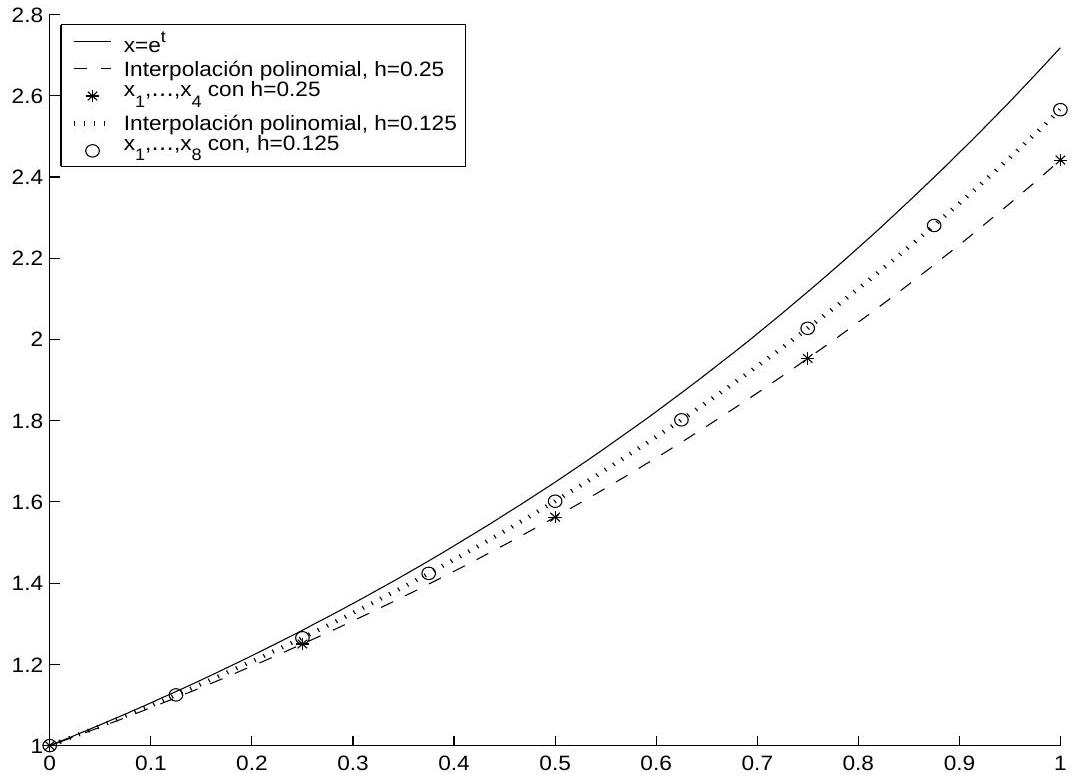
\includegraphics[width=\textwidth]{2025_09_05_3888c9ac96bd653d96b4g-175}
\captionsetup{labelformat=empty}
\caption{Figura 8.1. Método de Euler, \$x\^{}\{\textbackslash prime}=x ; x(0)=1\$; con pasos $h=0,25$ y $h=0,125$.\}\end{center}
\end{figure}

$$
x_{n}=\left(1+\frac{1}{n}\right)^{n}
$$

de la que sabemos que $\lim _{n \rightarrow \infty}\left(1+\frac{1}{n}\right)^{n}=e$.\\
La Tabla 8.1 muestra los valores que se obtienen si se usa el método ed Euler con paso $h=0,25$ y paso $h=0,125$. Estos datos pueden apreciarse en la Figura 8.1.

\begin{center}
\begin{tabular}{|l|l|l|l|}
\hline
$t$ & $e^{t}$ & $h=0,25$ & $h=0,125$ \\
\hline
0.125 & 1.1331 &  & 1.125000 \\
0.250 & 1.2840 & 1.250000 & 1.265625 \\
0.375 & 1.4549 &  & 1.423828 \\
0.500 & 1.6487 & 1.562500 & 1.601807 \\
0.625 & 1.8682 &  & 1.802032 \\
0.750 & 2.1170 & 1.953125 & 2.027207 \\
0.875 & 2.3989 &  & 2.280697 \\
1.000 & 2.7183 & 2.441406 & 2.565784 \\
\hline
\end{tabular}
\end{center}

Cuadro 8.1. Método de Euler, $x^{\prime}=x ; x(0)=1$; con paso $h=0,25$ y $h=0,125$

El método general de un paso tiene la forma


\begin{equation*}
x_{i+1}=x_{i}+h \Phi\left(t_{i}, x_{i}, h\right) \tag{8.4}
\end{equation*}


La función $\Phi$ se conoce como la función de incremento y nos dice como calcular la aproximación $x_{i+1}$ de $x\left(t_{i}+h\right)$ a partir de $x_{i}, t_{i}$ y de $h$. Una ventaja de estos métodos es que se puede cambiar fácilmente el paso $h$. Es decir calculamos una aproximación en un tiempo posterior $t_{i+1}$ a partir de una aproximación en el tiempo $t_{i}$. Notar que el método de Euler (8.3) corresponde con (8.4) para $\Phi(t, x, h)=f(t, x)$.\\
1.2. Métodos de Taylor. El método de Euler dado en (8.3) consiste en aproximar la función $x(t)$ por su polinomio de Taylor de grado uno. En efecto,

$$
x(t+h)=x(t)+x^{\prime}(t) h+x^{\prime \prime}(\xi) \frac{h^{2}}{2},
$$

donde $\xi$ está entre $t$ y $t+h$. Si $h$ es pequeño se puede despreciar el término $x^{\prime \prime}(\xi) \frac{h^{2}}{2}$ obteniendo


\begin{equation*}
x(t+h) \sim x(t)+x^{\prime}(t) h=x(t)+h f(t, x(t)) . \tag{8.5}
\end{equation*}


El método de Euler (8.3) en el paso $i+1$ se basa en utilizar (8.5) desarrollado en $t=t_{i}$ reemplazando el valor desconocido $x\left(t_{i}\right)$ por su aproximación $x_{i}$.

Este método se puede generalizar utilizando desarrollos de mayor orden dando lugar a los llamados métodos de Taylor de orden $k$. Recordemos que para valores de $h$ pequeños se tiene


\begin{equation*}
x(t+h)=x(t)+h x^{\prime}(t)+\frac{1}{2} h^{2} x^{\prime \prime}(t)+\cdots+\frac{1}{k!} h^{k} x^{(k)}(t)+\frac{1}{(k+1)!} h^{k+1} x^{(k+1)}(\xi) \tag{8.6}
\end{equation*}


donde $\xi$ está entre $t$ y $t+h$.\\
Como antes trabajamos en el intervalo $\left[t_{0}, T\right]$ y queremos dar una aproximación de $x(T)$. Elegi$\operatorname{mos} n \in \mathbb{N}$ y $t_{1}, \ldots, t_{n}$ puntos equiespaciados, $t_{i}=t_{0}+i h, i=0, \ldots, n$, con $h=\left(T-t_{0}\right) / n$.

Si conociéramos las derivadas de $x$ hasta orden $k$ en los valores $t_{i}$ podríamos usar esos datos para implementar un método que aproxime $x\left(t_{i}+h\right)$ a partir de una aproximación de $x\left(t_{i}\right)$. La ecuación diferencial $x^{\prime}(t)=f(t, x(t))$ nos proporciona las derivadas de orden superior. Por ejemplo para hallar $x^{\prime \prime}$ derivamos $x^{\prime}$ y obtenemos

$$
x^{\prime \prime}(t)=f_{t}(t, x(t))+f_{x}(t, x(t)) x^{\prime}(t)
$$

es decir,

$$
x^{\prime \prime}(t)=f_{t}(t, x)+f_{x}(t, x(t)) f(t, x(t)) .
$$

Con la segunda derivada de $x$ podemos hacer el desarrollo de orden 2. Suponemos hallados los valores de $x_{j}$ que aproximan $x\left(t_{j}\right)$ para $j=1, \ldots, i$, entonces para $t_{i+1}=t_{i}+h$ se tiene

$$
x\left(t_{i}+h\right) \sim x\left(t_{i}\right)+h f\left(t_{i}, x\left(t_{i}\right)\right)+\frac{1}{2} h^{2}\left[f_{t}\left(t_{i}, x\left(t_{i}\right)\right)+f_{x}\left(t_{i}, x\left(t_{i}\right)\right) f\left(t_{i}, x\left(t_{i}\right)\right)\right] .
$$

De acuerdo con esta fórmula, el método de aproximación es


\begin{equation*}
x_{i+1}=x_{i}+h f\left(t_{i}, x_{i}\right)+\frac{1}{2} h^{2}\left[f_{t}\left(t_{i}, x_{i}\right)+f_{x}\left(t_{i}, x_{i}\right) f\left(t_{i}, x_{i}\right)\right] . \tag{8.7}
\end{equation*}


La fórmula de iteración (8.7) se conoce con el nombre de Método de Taylor de orden 2 y corresponde a la expresión (8.4) si consideramos $\Phi(t, x, h)=f(t, x)+\frac{h}{2}\left[f_{t}(t, x)+f_{x}(t, x) f(t, x)\right]$.

El método de Taylor de orden 3 se consigue derivando $x^{\prime \prime}$. En lo que sigue escribimos simplemente $x$ en lugar de $x(t)$. La fórmula para $x^{\prime \prime \prime}$ queda en términos de $f$ y sus derivadas,

$$
\begin{aligned}
x^{\prime \prime \prime}(t)= & f_{t t}(t, x)+2 f_{t x}(t, x) f(t, x)+f_{x x}(t, x) f^{2}(t, x) \\
& +f_{t}(t, x) f_{x}(t, x)+f_{t}^{2}(t, x) f(t, x)
\end{aligned}
$$

Continuando de esta manera se pueden calcular las derivadas de $x$ hasta orden $k$ en términos de $f$ y sus derivadas. Esto nos da una manera de calcular métodos de aproximación de un paso (solo usamos $t_{i}, x_{i}$ y $h$ para calcular la siguiente aproximación $x_{i+1}$ ).

Para formalizar este procedimiento introducimos dos notaciones. Llamamos $D^{j} f$ a la derivada total de $f$ respecto de $t$, es decir

$$
D^{j} f(t, x)=\frac{d^{(j)}}{d t} f(t, x(t))
$$

Por ejemplo, si $j=0, D^{0} f(t, x)=f(t, x)$ y para $j=1, D^{1} f(t, x)=f_{t}(t, x)+f_{x}(t, x) f(t, x)$.\\
Ahora, ponemos


\begin{equation*}
T_{k}(t, x, h)=\sum_{j=1}^{k} \frac{h^{j-1}}{j!} D^{j} f(t, x) \tag{8.8}
\end{equation*}


Así, de (8.6) obtenemos la aproximación

$$
x(t+h) \sim x(t)+h T_{k}(t, x, h)
$$

de donde se tiene la siguiente fórmula de recurrencia,

$$
x_{i+1}=x_{i}+h T_{k}\left(t_{i}, x_{i}, h\right)
$$

Estos métodos se conocen como métodos de Taylor de orden $k$. Su mayor problema es que requieren encontrar y evaluar derivadas sucesivas de $f(t, x)$.

Ejemplo 8.4. Aplicar el método de Euler y Taylor de orden 2 para el problema

$$
\left\{\begin{array}{l}
x^{\prime}(t)=\frac{t+2}{t+1} x \\
x(0)=1
\end{array}\right.
$$

Conocemos la solución exacta que corresponde a la función $x(t)=(t+1) e^{t}$. En efecto, $x(0)=1$ y $x^{\prime}(t)=(t+2) e^{t}=(t+2) \frac{x(t)}{(t-1)}$. Esto nos va a permitir comparar las aproximaciones obtenidas con los valores reales de $x(t)$ como muestra la Figura 8.2.

Empezamos escribiendo la iteración que se obtiene usando el método de Euler.

$$
\left\{\begin{array}{l}
x_{0}=1 \\
x_{i+1}=x_{i}+h \frac{t_{i}+2}{t_{i}+1} x_{i}
\end{array}\right.
$$

Para el método de Taylor de orden 2 necesitamos conocer $x^{\prime \prime}$ en términos de $(t, x)$. Al derivar $x^{\prime}$, se obtiene

$$
x^{\prime \prime}=\frac{-1}{(t+1)^{2}} x+\frac{t+2}{t+1} x^{\prime}=\frac{t^{2}+4 t+3}{(t+1)^{2}} x
$$

Entonces, la iteración del método de orden 2 es

$$
\left\{\begin{array}{l}
x_{0}=1 \\
x_{i+1}=x_{i}+h \frac{t_{i}+2}{t_{i}+1} x_{i}+\frac{h^{2}}{2}\left[\frac{t_{i}^{2}+4 t_{i}+3}{\left(t_{i}+1\right)^{2}} x_{i}\right]
\end{array}\right.
$$

Para dar una tabla de valores, en ambos casos, consideramos $h=0,25$ con lo cual $t=(0,0,25,0,5,0,75,1)$

\begin{center}
\begin{tabular}{|l|l|l|l|}
\hline
$t$ & $x=(t+1) e^{t}$ & Euler & Taylor 2 \\
\hline
0.000 & 1.000000 & 1.000000 & 1.000000 \\
0.250 & 1.605032 & 1.500000 & 1.593750 \\
0.500 & 2.473082 & 2.175000 & 2.440430 \\
0.750 & 3.704750 & 3.081250 & 3.635223 \\
1.000 & 5.436564 & 4.291741 & 5.306777 \\
\hline
\end{tabular}
\end{center}

Cuadro 8.2. Métodos de Euler y Taylor orden $2, x^{\prime}=\frac{t+2}{t+1} x ; x(0)=1$; paso $h=0,25$.

Con estos valores tenemos el gráfico que muestra la Figura 8.2.\\
1.3. Métodos de Runge-Kutta. Los métodos de un paso más usados son los que se conocen como de Runge-Kutta. La idea es obtener aproximaciones que resulten del mismo orden que las que se obtienen con los métodos de Taylor, pero sin tener que calcular derivadas de $f$.

Veamos cómo se deducen los métodos de Runge-Kutta de orden 2. Recordemos, ver (8.6), que el método de Taylor de orden 2 se basa en la igualdad

$$
x(t+h)=x(t)+h T_{2}(t, x(t), h)+O\left(h^{3}\right) .
$$

Ahora buscamos $\Phi_{2}(t, x, h)$ que no involucre cálculo de derivadas de $f$ y que cumpla

$$
x(t+h)=x(t)+h \Phi_{2}(t, x(t), h)+O\left(h^{3}\right) .
$$

\begin{figure}[h]
\begin{center}
  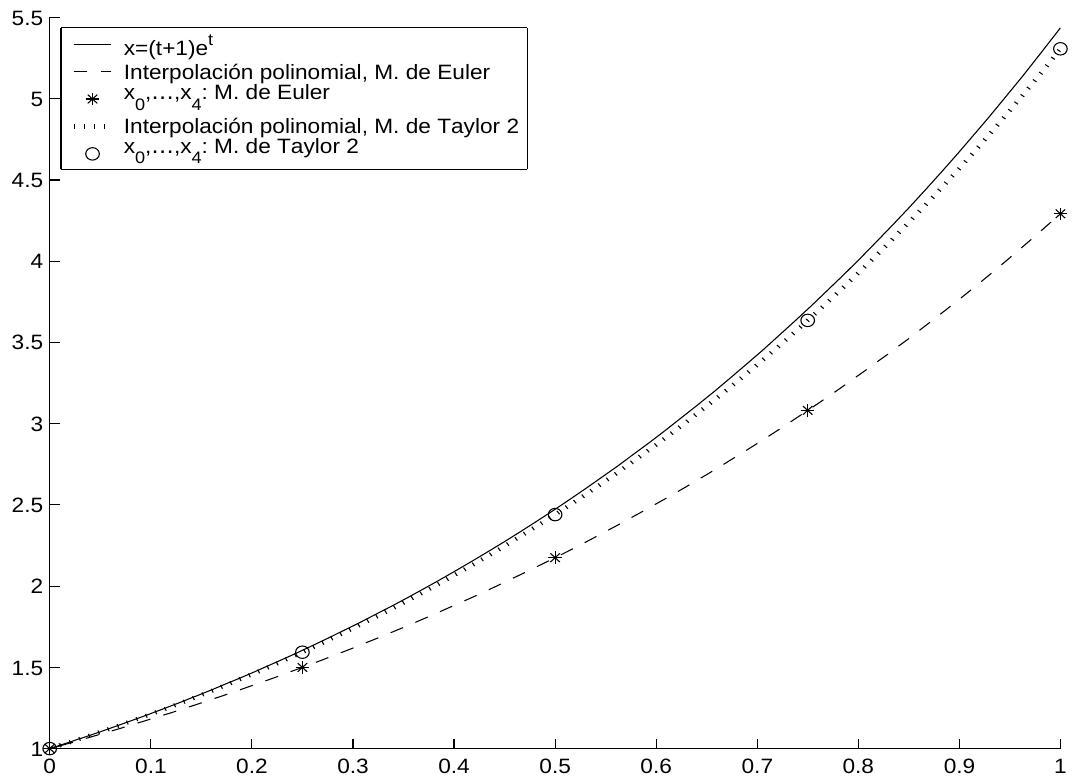
\includegraphics[width=\textwidth]{2025_09_05_3888c9ac96bd653d96b4g-179}
\captionsetup{labelformat=empty}
\caption{Figura 8.2. Métodos de Euler y Taylor orden 2, \$x\^{}\{\textbackslash prime}=\textbackslash frac\{t+2\}\{t+1\} x ; x(0)=1\$; paso $h=0,25$.\}\end{center}
\end{figure}

Para esto es suficiente que se cumpla


\begin{equation*}
T_{2}(t, x(t), h)-\Phi_{2}(t, x(t), h)=O\left(h^{2}\right) . \tag{8.9}
\end{equation*}


Buscamos $\Phi_{2}$ de la siguiente forma


\begin{equation*}
\Phi_{2}(t, x, h)=A_{1} f(t, x)+A_{2} f(t+\alpha h, x+\alpha h f(t, x)) \tag{8.10}
\end{equation*}


donde $A_{1}, A_{2}, \alpha$ son valores a determinar.\\
Observemos que es natural que a un incremento $\alpha h$ en la variable $t$ le corresponda un incremento $\alpha h x^{\prime}$ en la variable $x$, siendo $x^{\prime}=f(t, x)$.

Usando el desarrollo de Taylor para funciones de dos variables obtenemos

$$
f(t+\alpha h, x+\alpha h f(t, x))=f(t, x)+f_{t}(t, x) \alpha h+f_{x}(t, x) \alpha h f(t, x)+O\left(h^{2}\right) .
$$

Reemplazando en (8.10) tenemos

$$
\Phi_{2}(t, x, h)=\left(A_{1}+A_{2}\right) f(t, x)+A_{2} \alpha h\left[f_{t}(t, x)+f_{x}(t, x) f(t, x)\right]+O\left(h^{2}\right) .
$$

Como $T_{2}(t, x, h)=f(t, x)+\frac{1}{2} h\left[f_{t}(t, x)+f_{x}(t, x) f(t, x)\right.$ obtenemos (8.9) si pedimos

$$
A_{1}+A_{2}=1, \quad A_{2} \alpha=\frac{1}{2} .
$$

Despejando, se tiene

$$
A_{2}=\frac{1}{2 \alpha}, \quad A_{1}=1-\frac{1}{2 \alpha} .
$$

Es decir, hay infinitas soluciones dependiendo de $\alpha$ y por ende, infinitos métodos posibles de la forma

$$
x_{i+1}=x_{i}+h \Phi_{2}\left(t_{i}, x_{i}, h\right)
$$

para $\Phi_{2}(t, x, h)=\left(1-\frac{1}{2 \alpha}\right) f(t, x)+\frac{1}{2 \alpha} f(t+\alpha h, x+\alpha h f(t, x))$.\\
Eligiendo $\alpha=1 / 2$ se tiene $A_{1}=0, A_{2}=1$, lo que da lugar a la fórmula de recurrencia que se conoce como Método de Euler modificado,


\begin{equation*}
x_{i+1}=x_{i}+\frac{h}{2}\left[f\left(t_{i}+\frac{h}{2}, x_{i}+\frac{h}{2} f\left(t_{i}, x_{i}\right)\right)\right] . \tag{8.11}
\end{equation*}


Otra elección posible es $\alpha=1$. En este caso $A_{1}=A_{2}=\frac{1}{2}$ y se obtiene la iteración que se conoce como Método de Heun,


\begin{equation*}
x_{i+1}=x_{i}+\frac{h}{2}\left[f\left(t_{i}, x_{i}\right)+f\left(t_{i+1}, x_{i}+h f\left(t_{i}, x_{i}\right)\right)\right] . \tag{8.12}
\end{equation*}


En forma análoga a lo hecho para orden 2, se pueden considerar más términos en el desarrollo de Taylor y deducir métodos de Runge-Kutta de mayor orden. Específicamente, un método de Runge-Kutta de orden $k$ tiene la forma

$$
x_{i+1}=x_{i}+h \Phi_{k}\left(t_{i}, x_{i}, h\right)
$$

donde $\Phi_{k}$ verifica las siguientes dos condiciones


\begin{equation*}
T_{k}(t, x(t), h)-\Phi_{k}(t, x(t), h)=O\left(h^{k}\right) \tag{8.13}
\end{equation*}


siendo $T_{k}$ el operador definido en (8.8) y, además, es de la forma


\begin{equation*}
\Phi_{k}\left(t_{i}, x_{i}, h\right)=A_{1} f\left(\theta_{1}, \gamma_{1}\right)+\cdots+A_{N} f\left(\theta_{N}, \gamma_{N}\right) . \tag{8.14}
\end{equation*}


con ( $\theta_{i}, \gamma_{i}$ ) valores próximos a ( $t_{i}, x_{i}$ ). Para determinar el método que usamos es necesario especificar los $A_{i}$ y los puntos $\left(\theta_{i}, \gamma_{i}\right)$.

Se demuestra que puede obtenerse (8.13) para todo valor de $k$. Para $k=1,2,3$ y 4 , alcanza con tomar $N$ puntos en (8.14), con $N=k$. En cambio para $k>4$ es necesario tomar $N>k$, siendo suficiente tomar $N=k+1$ si $k=5,6$ y $N=k+2$ si $k \geq 7$.

A modo de ejemplo presentamos un método de Runge-Kutta de orden 4, que es uno de los más usados.


\begin{equation*}
x_{i+1}=x_{i}+\frac{h}{6}\left[K_{1}+2 K_{2}+2 K_{3}+K_{4}\right], \tag{8.15}
\end{equation*}


Donde,

$$
\begin{array}{ll}
K_{1}=f\left(t_{i}, x_{i}\right), & K_{3}=f\left(t_{i}+\frac{h}{2}, x_{i}+\frac{h}{2} K_{2}\right), \\
K_{2}=f\left(t_{i}+\frac{h}{2}, x_{i}+\frac{h}{2} K_{1}\right), & K_{4}=f\left(t_{i}+h, x_{i}+h K_{3}\right) .
\end{array}
$$

Ejemplo 8.5. Aplicar el método de Euler Modificado y el método de Runge-Kutta de orden 4 dado en (8.15) para aproximar $\sqrt{2}$ como solución del problema

$$
\left\{\begin{array}{l}
x^{\prime}(t)=\frac{1}{2 x} \\
x(1)=1
\end{array}\right.
$$

considerando el intervalo $[1,2]$.

En cualquier caso, la función a considerar es $f(t, x)=\frac{1}{2 x}$. Para el método de Euler Modificado la sucesión de recurrencias correspondiente a (8.10) es

$$
x_{i+1}=x_{i}+\frac{h}{2} \frac{1}{2 x_{i}+\frac{h}{2} \frac{1}{2 x_{i}}}=x_{i}+h \frac{x_{i}}{4 x_{i}^{2}+h}
$$

Para el método de orden 4 vamos a escribir $K_{1}, K_{2}, K_{3}$ y $K_{4} \sin$ desarrollar completamente las expresiones.

$$
\begin{array}{ll}
K_{1}=\frac{1}{2 x}, & K_{3}=\frac{1}{2 x+h K_{2}} \\
K_{2}=\frac{1}{2 x+h K_{1}}, & K_{4}=\frac{1}{2 x+h K_{3}}
\end{array}
$$

En la Tabla 8.3 damos los valores obtenidos con ambos métodos para un paso $h=0,25$. El gáfico correspondiente se tiene en la Figura 8.3.

\begin{center}
\begin{tabular}{|l|l|c|c|}
\hline
$t$ & $x=\sqrt{t}$ & Runge-Kutta 2 & Runge-Kutta 4 \\
\hline
1.000 & 1.000000 & 1.000000 & 1.000000 \\
1.250 & 1.118034 & 1.058824 & 1.119073 \\
1.500 & 1.224745 & 1.114734 & 1.226467 \\
1.750 & 1.322876 & 1.168117 & 1.325074 \\
2.000 & 1.414214 & 1.219278 & 1.416760 \\
\hline
\end{tabular}
\end{center}

Cuadro 8.3. Métodos de Runge-Kutta, $x^{\prime}=\frac{1}{2 x} ; x(1)=1$; paso $h=0,25$.

\section{Análisis del error y convergencia}
El objetivo de esta sección es analizar cuál es el error que se comete al utilizar los métodos numéricos para aproximar la solución de una ecuación de la forma (8.2). Para esto introducimos dos conceptos, el error de truncamiento local y el error global. El primero corresponde al error que se cometería al aproximar el valor de $x(t+h)$ si se conociera el valor exacto de $x(t)$, mientras que el segundo corresponde al error que se acumula al aplicar $n$ pasos de un método, es decir $x\left(t_{n}\right)-x_{n}$.

\begin{figure}[h]
\begin{center}
  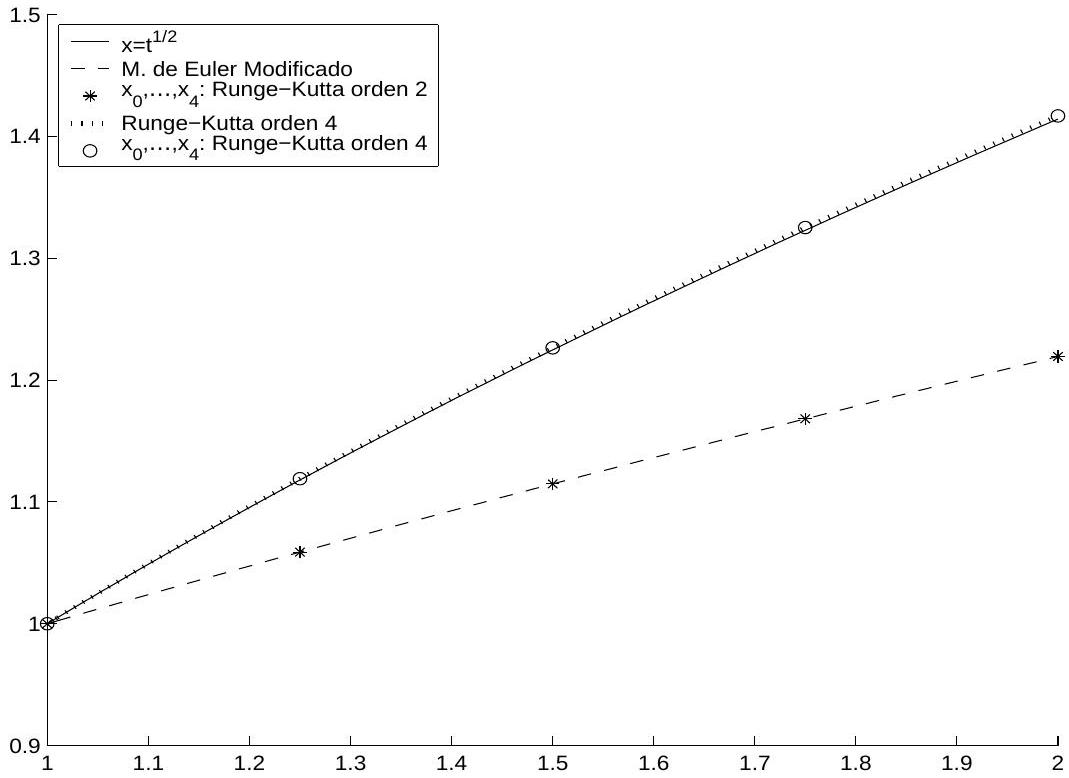
\includegraphics[width=\textwidth]{2025_09_05_3888c9ac96bd653d96b4g-182}
\captionsetup{labelformat=empty}
\caption{Figura 8.3. Métodos de Runge-Kutta, \$x\^{}\{\textbackslash prime}=\textbackslash frac\{1\}\{2 x\} ; x(1)=1\$; paso $h=0,25$.\}\end{center}
\end{figure}

2.1. Error de truncamiento local. Recordemos que un método general de un paso está dado por $x_{i+1}=x_{i}+h \Phi\left(t_{i}, x_{i}, h\right)$. Para estos métodos damos las siguientes definiciones

Definición 8.6. Llamaremos $\tau_{i}$ al error de truncamiento local que se comete en el paso $i$-ésimo. Este error está dado por la expresión:


\begin{equation*}
x\left(t_{i}+h\right)=x\left(t_{i}\right)+h \Phi\left(t_{i}, x\left(t_{i}\right), h\right)+h \tau_{i} . \tag{8.16}
\end{equation*}


Es decir,

$$
\tau_{i}=\tau\left(t_{i}, x\left(t_{i}\right), h\right)=\frac{x\left(t_{i}+h\right)-x\left(t_{i}\right)}{h}-\Phi\left(t_{i}, x\left(t_{i}\right), h\right) .
$$

Para simplificar la notación, cuando esto no genere confusión, llamaremos $\tau$ al error de truncamiento local en un $t$ genérico, es decir

$$
x(t+h)=x(t)+h \Phi(t, x(t), h)+h \tau .
$$

Definición 8.7. Diremos que el método es de orden $k$ si el error de truncamiento local satisface

$$
\tau=O\left(h^{k}\right) .
$$

Observemos que si usamos el desarrollo de Taylor de orden 1 obtenemos el error de truncamiento local del método de Euler. Sabemos que

$$
x(t+h)=x(t)+h x^{\prime}(t)+\frac{h^{2}}{2} x^{\prime \prime}(\xi) \quad \text { para algún } \xi \in(t, t+h) .
$$

Por otra parte la expresión (8.16) es de la forma

$$
x(t+h)=x(t)+h f(t, x(t))+h \tau
$$

de donde se sigue que


\begin{equation*}
\tau=\frac{h}{2} x^{\prime \prime}(\xi) \tag{8.17}
\end{equation*}


En general se tiene:\\
Proposición 8.8. El error de truncamiento local del método de Taylor de orden $k$ está dado por


\begin{equation*}
\tau=\frac{h^{k}}{(k+1)!} x^{(k+1)}(\xi), \text { para algún } \xi \in(t, t+h) . \tag{8.18}
\end{equation*}


En consecuencia, este método es efectivamente un método de orden $k$ de acuerdo con la Definición 8.7.

Demostración. Se sigue de la Definición 8.6 y de la fórmula del resto para el desarrollo de Taylor dada en (8.6).

Análogamente se obtiene el siguiente resultado para los métodos de Runge-Kutta.\\
Proposición 8.9. El error de truncamiento local de un método de de Runge-Kutta de orden $k$ verifica

$$
\tau=O\left(h^{k}\right)
$$

Demostración. Se sigue de la igualdad (8.13), es decir, $T_{k}(t, x(t), h)-\Phi_{k}(t, x(t), h)=O\left(h^{k}\right)$ y del error de truncamiento local de los métodos de Taylor, visto en la proposición anterior.\\
2.2. Error global. Si $x(t)$ es la solución de la ecuación

$$
\left\{\begin{array}{l}
x^{\prime}(t)=f(t, x(t)) \\
x\left(t_{0}\right)=x_{0}
\end{array}\right.
$$

estudiaremos, para $T>t_{0}$, cómo estimar el error que se comete al aproximar el valor de $x(T)$ utilizando métodos de un paso. En particular, veremos cómo depende este error del paso $h$.

Elegimos $n \in \mathbb{N}$ y $t_{1}, \ldots, t_{n}$ puntos equiespaciados, $t_{i}=t_{0}+i h, i=1, \ldots, n$, con $h=\left(T-t_{0}\right) / n$ de manera tal que $t_{n}=T$.

Teorema 8.10. Para $n \in \mathbb{N}$ y $h=\left(T-t_{0}\right) / n$ consideremos el método de un paso dado por

$$
x_{i+1}=x_{i}+h \Phi\left(t_{i}, x_{i}, h\right),
$$

con $\Phi$ una función Lipschitz en la segunda variable, o sea, existe una constante $K$ independiente de $t$ y h tal que


\begin{equation*}
|\Phi(t, x, h)-\Phi(t, y, h)| \leq K|x-y| \tag{8.19}
\end{equation*}


para todo $x, y \in \mathbb{R}$ y $t \in\left[t_{0}, T\right]$. Entonces, se tiene


\begin{equation*}
\left|x(T)-x_{n}\right| \leq \frac{\tau_{\text {máx }}}{K}\left(e^{K\left(T-t_{0}\right)}-1\right), \tag{8.20}
\end{equation*}


donde $\tau_{\text {máx }}=\operatorname{máx}_{1 \leq i \leq n}\left\{\left|\tau_{i}\right|\right\}$ con $\tau_{i}$ el error de truncamiento local del método en el paso $i$.

Demostración. Sea $e_{i}=x\left(t_{i}\right)-x_{i}$, el error global que se comete hasta el paso $i$.\\
Consideramos la ecuación del método y la definición de $\tau_{i}$ (8.16),

$$
\begin{aligned}
x_{i+1} & =x_{i}+h \Phi\left(t_{i}, x_{i}, h\right) \\
x\left(t_{i+1}\right) & =x\left(t_{i}\right)+h \Phi\left(t_{i}, x\left(t_{i}\right), h\right)+h \tau_{i}
\end{aligned}
$$

luego,

$$
e_{i+1}=x\left(t_{i+1}\right)-x_{i+1}=e_{i}+h\left(\Phi\left(t_{i}, x\left(t_{i}\right), h\right)-\Phi\left(t_{i}, x_{i}, h\right)\right)+h \tau_{i} .
$$

Usando que $\phi$ es Lipschitz se obtiene

$$
\begin{aligned}
\left|e_{i+1}\right| & \leq\left|e_{i}\right|+h\left|\Phi\left(t_{i}, x\left(t_{i}\right), h\right)-\Phi\left(t_{i}, x_{i}, h\right)\right|+h\left|\tau_{i}\right| \\
& \leq\left|e_{i}\right|+h K\left|x\left(t_{i}\right)-x_{i}\right|+h\left|\tau_{i}\right| \\
& \leq(1+K h)\left|e_{i}\right|+h\left|\tau_{i}\right| .
\end{aligned}
$$

Como $\left|\tau_{i}\right| \leq \tau_{\text {máx }}$, llamando $A=1+K h$, tenemos

$$
\left|e_{i+1}\right| \leq A\left|e_{i}\right|+h \tau_{\text {máx }} .
$$

Usando esta acotación para $i=0$ y teniendo en cuenta que $e_{0}=0$ se tiene

$$
\begin{aligned}
\left|e_{1}\right| & \leq h \tau_{\operatorname{máx}}, \\
\left|e_{2}\right| & \leq A\left|e_{1}\right|+h \tau_{\operatorname{máx}} \leq A h \tau_{\operatorname{máx}}+h \tau_{\operatorname{máx}}=(1+A) h \tau_{\operatorname{máx}} \\
\left|e_{3}\right| & \leq A\left|e_{2}\right|+h \tau_{\operatorname{máx}} \leq A(1+A) h \tau_{\operatorname{máx}}+h \tau_{\operatorname{máx}} \\
& =\left(A+A^{2}\right) h \tau_{\operatorname{máx}}+h \tau_{\operatorname{máx}} \\
& =\left(1+A+A^{2}\right) h \tau_{\operatorname{máx}}
\end{aligned}
$$

Iterando el procedimiento, podemos ver que

$$
\left|e_{n}\right| \leq\left(1+A+A^{2}+\cdots+A^{n-1}\right) h \tau_{\operatorname{máx}}=h \tau_{\operatorname{máx}} \sum_{j=0}^{n-1} A^{j}
$$

Ahora, usando la fórmula para suma de potencias tenemos

$$
\left|e_{n}\right| \leq h \tau_{\operatorname{máx}} \frac{A^{n}-1}{A-1}
$$

es decir

$$
\left|e_{n}\right| \leq h \tau_{\operatorname{máx}} \frac{(1+K h)^{n}-1}{K h}=\frac{\tau_{\operatorname{máx}}}{K}\left((1+K h)^{n}-1\right) \text {. }
$$

Como para $\alpha>0$ se tiene

$$
(1+\alpha)^{n} \leq e^{n \alpha}
$$

entonces,

$$
\left|e_{n}\right| \leq \frac{\tau_{\operatorname{máx}}}{K}\left(e^{n K h}-1\right)=\frac{\tau_{\operatorname{máx}}}{K}\left(e^{K\left(T-t_{0}\right)}-1\right),
$$

lo que concluye la demostración.

Bajo las hipótesis del Teorema 8.10 se deduce, de la fórmula (8.20), que un método de un paso es convergente si $\lim _{h \rightarrow 0} \tau_{\text {máx }}=0$. El resultado que sigue, del cual omitimos demostración permite verivicar facilmente si $\lim _{h \rightarrow 0} \tau_{\text {máx }}=0$.

Proposición 8.11. Para un método de un paso con función de incremento $\Phi$ continua en sus tres variables, se tiene que

$$
\lim _{h \rightarrow 0} \tau_{\text {máx }}=0 \quad \text { si y sólo si } \quad \Phi(t, x, 0)=f(t, x) \text {. }
$$

Observación 8.12. Los métodos de Euler, los de Taylor y de Rungge-Kutta son convergentes.

Demostración. Para los métodos de Taylor se tiene

$$
x\left(t_{i}+h\right) \sim x\left(t_{i}\right)+h x^{\prime}\left(t_{i}\right)+\frac{1}{2} h^{2} x^{\prime \prime}\left(t_{i}\right)+\cdots+\frac{1}{k!} h^{k} x^{(k)}\left(t_{i}\right)
$$

y por tanto

$$
\Phi(t, x, h)=x^{\prime}(t)+\frac{1}{2} h x^{\prime \prime}(t)+\cdots+\frac{1}{k!} h^{k-1} x^{(k)}(t)
$$

Al evaluar en $h=0$ tenemos, $\Phi(t, x, 0)=x^{\prime}(t)=f(t, x)$.\\
En cuanto a los métodos de Runge-Kutta, sólo verificaremos los dados por las fórmulas (8.11) y (8.12). El método de orden 4 dado por (8.15) queda como ejercicio.

Para Runge-Kutta de orden 2 tenemos:

Método de Euler modificado: $\quad x_{i+1}=x_{i}+h\left[f\left(t_{i}+\frac{h}{2}, x_{i}+\frac{h}{2} f\left(t_{i}, x_{i}\right)\right)\right]$,\\
Método de Heun: $\quad x_{i+1}=x_{i}+\frac{h}{2}\left[f\left(t_{i}, x_{i}\right)+f\left(t_{i+1}, x_{i}+h f\left(t_{i}, x_{i}\right)\right)\right]$.

Luego $\Phi(t, x, h)=f\left(t+\frac{h}{2}, x+\frac{h}{2} f(t, x)\right)$, y $\Phi(t, x, h)=\frac{1}{2}[f(t, x)+f(t, x+h f(t, x))]$ respectivamente. En ambos casos resulta

$$
\Phi(t, x, 0)=f(t, x) .
$$

Observación 8.13. El Teorema 8.10 requiere de la existencia de una constante de Lipschitz $K$ para la función de incremento $\Phi$. De existir una constante así, cualquier otra mayor también sirve para acotar el error utilizando la fórmula (8.20).

En los casos de los métodos de Runge-Kutta la hipótesis que $\Phi$ sea Lipschitz, condición (8.19), puede deducirse de que $f$ lo sea. Consideremos, por ejemplo, el método de Euler modificado (8.11), en un intervalo $[a, b]$.

Suponiendo que existe una constante $L$, tal que para todo $t \in[a, b]$

$$
|f(t, x)-f(t, y)| \leq L|x-y|,
$$

se tiene para $\Phi(t, x, h)=\frac{1}{2}\left[f\left(t+\frac{h}{2}, x+\frac{h}{2} f(t, x)\right)\right]$ que

$$
\begin{aligned}
|\Phi(t, x, h)-\Phi(t, y, h)| & \leq \frac{L}{2}\left|x-y+\frac{h}{2} f(t, x)-\frac{h}{2} f(t, y)\right| \\
& \leq \frac{L}{2}\left(|x-y|+L \frac{h}{2}|x-y|\right) .
\end{aligned}
$$

Como $h \leq b-a$, se tiene (8.19) para $\Phi$, con $K=\frac{1}{2}\left(L+L^{2}(b-a)\right)$.\\
Ejemplo 8.14. Se utiliza el método de Taylor de orden 2 con un paso $h<1$ para aproximar la solución del siguiente problema:

$$
\left\{\begin{array}{l}
x^{\prime}(t)=\operatorname{sen}(x(t))+\cos (x(t)), \\
x(2)=1
\end{array}\right.
$$

Hallar h para que el error cometido en $t=2,5$ sea menor que $10^{-4}$ y dar un valor de $n$ tal que el término $n$-ésimo de la iteración que da el método verifique que $\left|x_{n}-x(2,5)\right|<10^{-4}$.

Para estimar el error global necesitamos dar una constante Lipschitz para la función de incremento $\Phi$ y estimar el error de truncamiento local $\tau$.

Para conocer $\Phi$ calculamos $x^{\prime \prime}$. Como $x^{\prime}=\operatorname{sen}(x)+\cos (x)$ se tiene que

$$
x^{\prime \prime}=x^{\prime} \cos (x)-x^{\prime} \operatorname{sen}(x)=\cos ^{2}(x)-\operatorname{sen}^{2}(x)=\cos (2 x)
$$

Luego, $\Phi(t, x, h)=\operatorname{sen}(x)+\cos (x)+\frac{h}{2} \cos (2 x)$. Busquemos una constante de Lipschitz para $\Phi$. Usamos que $\Phi$ es derivable respecto de su segunda variable y ponemos $z$ un valor intermedio entre $x$ e $y$, así se tiene

$$
\begin{aligned}
|\Phi(t, x, h)-\Phi(t, y, h)| & =\left|\operatorname{sen}(x)+\cos (x)+\frac{h}{2} \cos (2 x)-\left[\operatorname{sen}(y)+\cos (y)+\frac{h}{2} \cos (2 y)\right]\right| \\
& =\left|\cos (z)-\operatorname{sen}(z)-2 \frac{h}{2} \operatorname{sen}(z)\right| \cdot|x-y| \\
& \leq[|\cos (z)|+|\operatorname{sen}(z)|+h|\operatorname{sen}(z)|]|x-y| \\
& \leq[2+h]|x-y|
\end{aligned}
$$

Ahora, para encontrar una constante independiente de $t$ y $h$ tenemos en cuenta el dato del enunciado $h<1$. Es decir, obtenemos

$$
|\Phi(t, x, h)-\Phi(t, y, h)| \leq 3|x-y|
$$

con lo cual elegimos $K=3$.\\
El paso siguiente es estimar $\tau$. Para esto necesitamos calcular $x^{\prime \prime \prime}$, lo hacemos usando la expresión de $x^{\prime \prime}$, es decir,

$$
\begin{gathered}
x^{\prime \prime \prime}=-2 x^{\prime} \operatorname{sen}(2 x)=-2[\operatorname{sen}(x)+\cos (x)] \operatorname{sen}(x) \\
|\tau|=\frac{h^{2}}{3!}\left|x^{\prime \prime \prime}(\xi)\right|=\left|2 \frac{h^{2}}{6}[\operatorname{sen}(x(\xi))+\cos (x(\xi))] \operatorname{sen}(x(\xi))\right| \leq \frac{2}{3} h^{2}
\end{gathered}
$$

De donde $\tau_{\text {máx }} \leq \frac{2}{3} h^{2}$. Finalmente, siendo $T=2,5$ y $t_{0}=2$ tenemos

$$
\left|e_{n}\right| \leq \frac{\tau_{\operatorname{máx}}}{K}\left(e^{K\left(T-t_{0}\right)}-1\right) \leq \frac{2}{3} \frac{h^{2}}{3}\left(e^{3(0,5)}-1\right) \leq \frac{2}{9} h^{2} 4<h^{2} .
$$

Como buscamos $h<1$ tal que el error cometido sea menor que $10^{-4}$ basta con tomar $h=10^{-2}$. Notar que cualquier $h$ más pequeño también sirve.

Para dar el valor de $n$ tal que $\left|x_{n}-x(2,5)\right|<10^{-4}$ recordemos que $\left(T-t_{0}\right) / n=h$. Luego, $n=0,5 / h=50$ sirve y cualquier $n>50$ también, ya si $n>50$ entonces $h<10^{-2}$.

Aplicación a sistemas de ecuaciones: Observemos que si en lugar de una ecuación tenemos un sistema de ecuaciones dado por

$$
\left\{\begin{array}{ccc}
x_{1}^{\prime}(t) & = & F_{1}\left(t, x_{1}(t), x_{2}(t), \ldots, x_{n}(t)\right), \\
x_{2}^{\prime}(t) & = & F_{2}\left(t, x_{1}(t), x_{2}(t), \ldots, x_{n}(t)\right), \\
\vdots & \vdots & \vdots \\
x_{n}^{\prime}(t) & = & F_{n}\left(t, x_{1}(t), x_{2}(t), \ldots, x_{n}(t)\right),
\end{array}\right.
$$

con valores iniciales $x_{1}\left(t_{0}\right)=a_{1}, \ldots, x_{n}\left(t_{0}\right)=a_{n}$, podemos pensar el problema en forma vectorial llamando $X(t)=\left(x_{1}(t), \ldots, x_{n}(t)\right)^{t}$, y $F$ el vector que tiene en la componente $i$-ésima la función $F_{i}(t, X(t))$. En este tipo de problemas usualmente la notación para los vectores es vertical. Esto nos permite escribir el sistema como sigue

$$
\left\{\begin{array}{l}
X^{\prime}(t)=F(t, X(t)), \\
X\left(t_{0}\right)=\left(a_{1}, \ldots, a_{n}\right)^{t} .
\end{array}\right.
$$

De esta manera, se pueden usar los métodos ya estudiados. Por ejemplo usando el método de Euler queda

$$
X_{i+1}=X_{i}+h F\left(t_{i}, X_{i}\right),
$$

donde $X_{i}$ es un vector de $n$-coordenadas, $i=1, \ldots, n$. En general, los métodos a un paso tienen la forma

$$
X_{i+1}=X_{i}+h \Phi\left(t_{i}, X_{i}, h\right) .
$$

Ejemplo 8.15. Se quiere dar la sucesión de recurrencias correspondientes al método de Euler para el sistema de ecuaciones

$$
\left\{\begin{array}{l}
x^{\prime}(t)=3 y(t)-2 t \cos (x(t)), \\
y^{\prime}(t)=x^{2}(t)-t y(t), \\
x(0)=-1, \quad y(0)=2 .
\end{array}\right.
$$

Notar que $F_{1}(t, x, y)=3 y-2 t \cos (x)$ y $F_{2}(t, x, y)=x^{2}-t y$. Para estas funciones el método viene dado por

$$
\binom{x_{i+1}}{y_{i+1}}=\binom{x_{i}}{y_{i}}+h \cdot\binom{F_{1}\left(t, x_{i}, y_{i}\right)}{F_{2}\left(t, x_{i}, y_{i}\right)}=\binom{x_{i}}{y_{i}}+h \cdot\binom{3 y_{i}-2 t_{i} \cos \left(x_{i}\right)}{x_{i}^{2}-t_{i} y_{i}}
$$

de modo que empezando con $x_{0}=-1, y_{0}=2$ el par de iteraciones del método de Euler viene dado por

$$
\left\{\begin{array}{l}
x_{i+1}=x_{i}+h\left(3 y_{i}-2 t_{i} \cos \left(x_{i}\right)\right), \\
y_{i+1}=y_{i}+h\left(x_{i}^{2}-t_{i} y_{i}\right) .
\end{array}\right.
$$

\section{Métodos multipaso lineales}
Hasta ahora para aproximar las soluciones de $x^{\prime}(t)=f(t, x(t))$ nos basamos en el punto inmediato anterior para calcular el siguiente, es decir, empezando en $x_{0}$ las iteraciones de un paso son de la forma

$$
x_{n+1}=x_{n}+h \Phi\left(t_{n}, x_{n}, h\right)
$$

La filosofía de los métodos multipaso es usar la información obtenida hasta el momento (varias aproximaciones anteriores a la que se quiere calcular). Es decir, se quiere aproximar $x$ en el paso ( $n+1$ )-ésimo, $x\left(t_{n+1}\right)$, utilizando algunos de los valores ya calculados como $x_{n}, x_{n-1}, x_{n-2}, \ldots$ Si se considera un registro de $k$ datos anteriores el método tiene la forma:


\begin{equation*}
\alpha_{k} x_{n+k}=-\sum_{j=0}^{k-1} \alpha_{j} x_{n+j}+h \sum_{j=0}^{k} \beta_{j} f\left(t_{n+j}, x_{n+j}\right) \tag{8.21}
\end{equation*}


Un método como en (8.21) se conoce como método multipaso de $k$ pasos.

Por ejemplo, si aproximamos la derivada por

$$
x^{\prime}(t) \sim \frac{x(t+h)-x(t-h)}{2 h}
$$

considerando puntos equiespaciados nos queda

$$
x^{\prime}\left(t_{n}\right) \sim \frac{x_{n+1}-x_{n-1}}{2 h}
$$

y como

$$
x^{\prime}\left(t_{n}\right)=f\left(t_{n}, x\left(t_{n}\right)\right) \sim f\left(t_{n}, x_{n}\right)
$$

podemos poner

$$
\frac{x_{n+1}-x_{n-1}}{2 h}=f\left(t_{n}, x_{n}\right)
$$

es decir

$$
x_{n+1}=x_{n-1}+2 h f\left(t_{n}, x_{n}\right)
$$

Éste, resulta ser un método de dos pasos puesto que para calcular $x_{n+1}$ se usan $x_{n}$ y $x_{n-1}$.

Los métodos de integración también nos proporcionan ejemplos de métodos multipaso. Por ejemplo, partimos del cálculo de la integral

$$
x\left(t_{n+2}\right)-x\left(t_{n}\right)=\int_{t_{n}}^{t_{n+2}} x^{\prime}(s) d s
$$

y aproximamos el valor de la integral por la regla de Simpson, obteniendo

$$
x\left(t_{n+2}\right)-x\left(t_{n}\right) \sim \frac{h}{3}\left(x^{\prime}\left(t_{n}\right)+4 x^{\prime}\left(t_{n+1}\right)+x^{\prime}\left(t_{n+2}\right)\right) .
$$

Como estamos resolviendo la ecuación $x^{\prime}(t)=f(t, x(t))$ podemos proponer el siguiente método

$$
x_{n+2}-x_{n}=\frac{h}{3}\left(f\left(t_{n}, x_{n}\right)+4 f\left(t_{n+1}, x_{n+1}\right)+f\left(t_{n+2}, x_{n+2}\right)\right)
$$

que es un método de dos pasos.\\
En adelante, pondremos $f_{n}$ por $f\left(t_{n}, x_{n}\right)$. Con esta notación, los métodos multipaso de $k$ pasos admiten la escritura


\begin{equation*}
\sum_{j=0}^{k} \alpha_{j} x_{n+j}=h \sum_{j=0}^{k} \beta_{j} f_{n+j}, \tag{8.22}
\end{equation*}


donde $h$ es la distancia entre dos nodos, $\alpha_{j}$ y $\beta_{j}$ son coeficientes conocidos y $\alpha_{k} \neq 0$.\\
Si $\beta_{k} \neq 0$, el término $\beta_{k} f_{n+k}$ aparece en la suma de la derecha con lo cuál el valor a calcular $x_{n+k}$ aparece involucrado en la ecuación en la evaluación de $f$. Por este motivo se dice que el método es implícito.

Cuando $\beta_{k}=0$ el valor a encontrar $x_{n+k}$ se puede despejar de datos ya conocidos y el método se dice explícito.

Con los ejemplos vistos hasta ahora tenemos que,


\begin{equation*}
x_{n+2}-x_{n}=\frac{h}{3}\left(f_{n}+4 f_{n+1}+f_{n+2}\right) \tag{8.23}
\end{equation*}


es un método implícito, que se conoce como el método de Milne, mientras que el que resulta de aproximar la derivada

$$
x_{n+2}=x_{n}+2 h f_{n+1}
$$

es un método de dos pasos explícito.\\
Si usamos una fórmula de cuadratura basada en interpolación de Lagange para aproximar la integral $\int_{t_{n+k-1}}^{t_{n+k}} x^{\prime}(s) d s$,

$$
\int_{t_{n+k-1}}^{t_{n+k}} x^{\prime}(s) d s \sim h\left[A_{0} x^{\prime}\left(t_{n}\right)+\cdots+A_{k} x^{\prime}\left(t_{n+k}\right)\right]
$$

obtenemos métodos de la forma,

$$
x_{n+k}-x_{n+k-1}=h\left[A_{0} f_{n}+\cdots+A_{k} f_{n+k}\right]
$$

Los explícitos se conocen como métodos de Adams-Bashforth y los implícitos como métodos de Adams-Moulton (ver ejercicios).

Para comenzar a aplicar los métodos multipaso se necesitan los primeros $k$ valores que usualmente se calculan con métodos a un paso.

Ejemplo 8.16. Verificar que el método de Adams-Bashforth de 3 pasos está dado por

$$
x_{n+3}-x_{n+2}=\frac{h}{12}\left(23 f_{n+2}-16 f_{n+1}+5 f_{n}\right) .
$$

La fórmula de cuadratura a utilizar será de la forma

$$
A x^{\prime}\left(t_{n+2}\right)+B x^{\prime}\left(t_{n+1}\right)+C x^{\prime}\left(t_{n}\right) .
$$

Ejemplo 8.17. Se quiere dar un método de multipaso que provenga de aproximar $\int_{t_{n+1}}^{t_{n+3}} x^{\prime}(t) d t$, con una fórmula de cuadratura que utilice los nodos $\left\{t_{n}, t_{n+1}, t_{n+2}\right\}$.

La fórmula de cuadratura será

$$
A x^{\prime}\left(t_{n}\right)+B x^{\prime}\left(t_{n+1}\right)+C x^{\prime}\left(t_{n+2}\right) .
$$

Para facilitar el cálculo de los coeficientes $A, B, C$, trasladamos linealmente la situación a un intervalo conocido y buscamos la regla de cuadratura en dicho intervalo.

Los valores de $t$ considerados son $\left\{t_{n}, t_{n+1}, t_{n+2}, t_{n+3}\right\}$ que además son equiespaciados, entonces podemos considerar en su lugar lo nodos $\{-1,0,1,2\}$. El problema se reduce a resolver el sistema de ecuaciones

$$
\left\{\begin{aligned}
\tilde{A}+\tilde{B}+\tilde{C} & =2 \\
-\tilde{A}++\tilde{C} & =2 \\
\tilde{A}++\tilde{C} & =\frac{8}{3}
\end{aligned}\right.
$$

con $\tilde{A}, \tilde{B}, \tilde{C}$ los coeficientes correspondientes a la cuadratura en $[0,2]$, exacta para $\left\{1, t, t^{2}\right\}$. Puede verse que $\left\{\frac{1}{3},-\frac{2}{3}, \frac{7}{3}\right\}$ son los valores buscados, es decir

$$
\int_{0}^{2} g(s) d s \sim \frac{1}{3} g(-1)-\frac{2}{3} g(0)+\frac{7}{3} g(1)
$$

Ahora,

$$
\int_{t_{n+1}}^{t_{n+3}} x^{\prime}(t) d t=\int_{0}^{2} x^{\prime}(a s+b) a d s
$$

donde $a, b$ corresponden al corrimiento $t=a s+b$ :

$$
\left\{\begin{array} { l } 
{ s = 0 \rightarrow t = t _ { n + 1 } = t _ { n } + h } \\
{ s = 2 \rightarrow t = t _ { n + 3 } = t _ { n } + 3 h }
\end{array} \Rightarrow \left\{\begin{array}{l}
a=h \\
b=t_{n}+h
\end{array} .\right.\right.
$$

Es decir,

$$
\int_{t_{n+1}}^{t_{n+3}} x^{\prime}(t) d t \sim h\left[\frac{1}{3} x^{\prime}\left(t_{n}\right)-\frac{2}{3} x^{\prime}\left(t_{n+1}\right)+\frac{7}{3} x^{\prime}\left(t_{n+2}\right)\right]
$$

Ahora, como $x^{\prime}\left(t_{n}\right)=f\left(t_{n}, x\left(t_{n}\right)\right)$ se aproxima por $f_{n}=f\left(t_{n}, x_{n}\right)$ y además

$$
x\left(t_{n+3}\right)-x\left(t_{n+1}\right) \sim h\left[\frac{1}{3} x^{\prime}\left(t_{n}\right)-\frac{2}{3} x^{\prime}\left(t_{n+1}\right)+\frac{7}{3} x^{\prime}\left(t_{n+2}\right)\right],
$$

proponemos el método

$$
x_{n+3}-x_{n+1}=h\left[\frac{1}{3} f_{n}-\frac{2}{3} f_{n+1}+\frac{7}{3} f_{n+2}\right],
$$

que es un método de multipaso explícito de 3 pasos.\\
3.1. Convergencia de los métodos multipaso. Empecemos estudiando el error de truncamiento local para un método de $k$ pasos. Para esto, recordemos que en los métodos de 1 paso de la forma

$$
x_{i+1}=x_{i}+h \Phi\left(t_{i}, x_{i}, h\right),
$$

el error local es $\tau$ definido por medio de la expresión

$$
x(t+h)-x(t)-h \Phi(t, x(t), h)=h \tau
$$

donde $x$ es la solución exacta del problema $x^{\prime}(t)=f(t, x(t))$. Sabemos que el método resulta convergente cuando $\tau$ tiende a cero. Aplicando la misma idea para un método de $k$ pasos de la forma

$$
\sum_{j=0}^{k} \alpha_{j} x_{n+j}=h \sum_{j=0}^{k} \beta_{j} f_{n+j}
$$

teniendo en cuenta que $x^{\prime}=f$, definimos $\tau$, el error de truncamiento local, de la siguiente manera


\begin{equation*}
\sum_{j=0}^{k} \alpha_{j} x(t+j h)-h \sum_{j=0}^{k} \beta_{j} x^{\prime}(t+j h)=h \tau . \tag{8.24}
\end{equation*}


Vamos a ver que para los métodos multipaso no es suficiente pedir que $\tau$ tienda a cero para que el método sea convergente. En este caso serán dos las condiciones (consistencia y estabilidad) que aseguren la convergencia de $x_{n+k}$ a la solución exacta.\\
Definición 8.18. Se dice que un método multipaso es consistente si el error de truncamiento local, $\tau$, tiende a cero.

En forma análoga a la Definición 8.7 de orden para los métodos de un paso, se tiene que un método multipaso es de orden $p$ si $\tau=O\left(h^{p}\right)$.

En lo que sigue, estudiaremos un algoritmo que nos permite establecer el orden de un método multipaso. Para esto, necesitamos asumir que $x$, la solución de la ecuación diferencial $x^{\prime}=f(t, x)$ admite $p+1$ derivadas continuas. En tal caso, de la expresión (8.24) se puede escribir $h \tau$ en términos de las derivadas de $x$ como sigue


\begin{equation*}
h \tau=C_{0} x(t)+C_{1} h x^{\prime}(t)+C_{2} h^{2} x^{\prime \prime}(t)+\cdots+C_{p} h^{p} x^{(p)}(t)+O\left(h^{p+1}\right) \tag{8.25}
\end{equation*}


En efecto, consideremos el desarrollo de Taylor para $x$ y $x^{\prime}$,

$$
\left\{\begin{aligned}
x(t+j h) & =x(t)+x^{\prime}(t) j h+\frac{x^{\prime \prime}(t)}{2}(j h)^{2}+\cdots \\
x^{\prime}(t+j h) & =x^{\prime}(t)+x^{\prime \prime}(t) j h+\frac{x^{\prime \prime \prime}(t)}{2}(j h)^{2}+\cdots
\end{aligned}\right.
$$

Ahora, reemplazamos en la expresión (8.24) y agrupamos las potencias de $h$. De esta forma, se obtiene (8.25) con

$$
\begin{aligned}
C_{0} & =\alpha_{0}+\cdots+\alpha_{k} \\
C_{1} & =\alpha_{1}+2 \alpha_{2}+3 \alpha_{3}+\cdots+k \alpha_{k}-\beta_{0}-\beta_{1}-\beta_{2}-\cdots-\beta_{k}
\end{aligned}
$$

y en general para cualquier $q \geq 1$,


\begin{equation*}
C_{q}=\frac{1}{q!}\left(\alpha_{1}+2^{q} \alpha_{2}+3^{q} \alpha_{3}+\cdots+k^{q} \alpha_{k}\right)-\frac{1}{(q-1)!}\left(\beta_{1}+2^{q-1} \beta_{2}+\cdots+k^{q-1} \beta_{k}\right) . \tag{8.26}
\end{equation*}


De la expresión (8.26) se obtiene inmediatamente\\
Proposición 8.19. Para un método de multipaso se tiene\\
i) El método es consitente si y sólo si $C_{0}=C_{1}=0$.\\
i) El método es de orden $p$ si y sólo si los valores $C_{q}, q \geq 1$ definidos por (8.26) verifican $C_{0}=C_{1}=\cdots=C_{p}=0$ y $C_{p+1} \neq 0$.\\
si método es de orden $p$ el error $\tau$ satisface

$$
\tau h=C_{p+1} h^{p+1} x^{(p+1)}(t)+O\left(h^{p+2}\right) .
$$

Para ver la convergencia, como antes, fijamos $T$ y ponemos $n$ y $h$ tales que $T=(n+k) h$. (Notar que estamos considerando el intervalo $[0, T]$.) Queremos

$$
\lim _{h \rightarrow 0} x_{n+k}=x(T) .
$$

Veremos qué condiciones debemos imponer al método para que esto ocurra.

Primero pongamos el problema $x^{\prime}(t)=0, x(0)=1$ (solución $x \equiv 1$ ). El método aplicado a este problema se reduce a

$$
\sum_{j=0}^{k} \alpha_{j} x_{n+j}=0 .
$$

Para cualquier método multipaso debemos tener (como $k$ está fijo y $h \rightarrow 0$ ) que los $k$ pasos del método sean convergentes, es decir, $x_{n+k} \rightarrow x(T), \ldots, x_{n} \rightarrow x(T)$. Entonces podemos escribir $x_{n+j}=x(T)+\varphi_{j}(h)$ con $\varphi_{j}(h) \rightarrow 0$ cuando $h \rightarrow 0$.

Usando esto se obtiene

$$
\sum_{j=0}^{k} \alpha_{j} x(T)+\sum_{j=0}^{k} \alpha_{j} \varphi_{j}(h)=0 .
$$

Como la segunda suma tiende a cero con $h$ tenemos que, $x(T) \sum_{j=0}^{k} \alpha_{j}=0$.\\
Es decir

$$
C_{0}=0 .
$$

Para que el método converja, también debe ser $C_{1}=0$. Para ver esto consideremos el problema $x^{\prime}(t)=1, x(0)=0$ que tiene como solución $x(t)=t$. El método para este problema se reduce a

$$
\sum_{j=0}^{k} \alpha_{j} x_{n+j}=h \sum_{j=0}^{k} \beta_{j}
$$

Es fácil verificar que la sucesión dada por

$$
x_{l}=\operatorname{lh} M
$$

es solución de este esquema donde

$$
M=\frac{\sum_{j=0}^{k} \beta_{j}}{\sum_{j=0}^{k} j \alpha_{j}}
$$

Si los valores iniciales se eligen de la forma $x_{l}=l h M$ el método va a producir la solución $x_{l}=l h M$ y en particular

$$
x_{n+k}=(n+k) h M
$$

Como suponemos que el método es convergente se tiene que lo valores iniciales satisfacen $x_{i} \rightarrow x(0)=0$ cuando $h \rightarrow 0$, y además $x_{n+k} \rightarrow x(T)$, pero

$$
x_{n+k}=(n+k) h M=T M \rightarrow T
$$

Entonces concluimos que

$$
M=1
$$

lo que nos da

$$
C_{1}=0 .
$$

Esto se denomina consistencia del método multipaso.\\
Un método de multipaso de $k$ pasos, $\sum_{j=0}^{k} \alpha_{j} x_{n+j}=h \sum_{j=0}^{k} \beta_{j} f_{n+j}$, tiene asociados dos polinomios


\begin{equation*}
p(z)=\sum_{j=0}^{k} \alpha_{j} z^{j} \quad \text { y } \quad q(z)=\sum_{j=0}^{k} \beta_{j} z^{j} . \tag{8.27}
\end{equation*}


Con esta notación podemos enunciar el siguiente resultado.\\
Proposición 8.20. Si p y q son los polinmios definidos en (8.27), la consistencia de un método de multipaso de $k$ pasos está dado por las condiciones:

$$
p(1)=0, \quad p^{\prime}(1)=q(1)
$$

Para los métodos de un paso, la consistencia implicaba la convergencia, para los métodos multipaso se requiere una condición adicional la condición de la raíz.

Veamos esto. Ahora consideremos el problema $x^{\prime}(t)=0, x(t)=0$, cuya solución es $x(t) \equiv 0$.\\
En este caso el método se reduce a

$$
\sum_{j=0}^{k} \alpha_{j} x_{n+j}=0 .
$$

Esto describe una ecuación en diferencias que admite como solución a la sucesión

$$
x_{m}=h r_{i}^{m}
$$

donde $r_{i}$ es cualquiera de las raíces del polinomio $p(z)$ dado en (8.27).\\
Si asumimos que el método es convergente se tiene que

$$
x_{n+k} \rightarrow x(T)=0 \quad h \rightarrow 0 .
$$

Además

$$
x_{n+k}=h\left(r_{i}\right)^{n+k} .
$$

Para verificar que $x_{n+k} \rightarrow 0$, como $n=T / h \rightarrow \infty$ cuando $h \rightarrow 0$ se debe tener que

$$
\left|r_{i}\right| \leq 1 .
$$

Entonces la convergencia implica que todo cero de $p(z)$ debe satisfacer

$$
\left|r_{i}\right| \leq 1 .
$$

Además, si $r_{i}$ es una raíz múltiple de $p(z)$ podemos poner

$$
x_{j}=h j^{q}\left(r_{i}\right)^{j}
$$

con $q \leq m-1$ ( $m$ es la multiplicidad de la raíz). Tenemos

$$
x_{n+k}=h(n+k)^{q} r_{i}^{n+k}
$$

y como $h(n+k)=T$ para que $x_{n+k} \rightarrow 0$ se debe tener

$$
\left|r_{i}\right|<1 .
$$

Las condiciones que acabamos de analizar para la convergencia de un método de multipaso se pueden resumen en la siguiente

Condición 8.21. (de la raíz)

\begin{enumerate}
  \item $\left|r_{i}\right| \leq 1$ si $r_{i}$ es un cero simple de $p(r)$.
  \item $\left|r_{i}\right|<1$ si $r_{i}$ es un cero múltiple de $p(r)$.
\end{enumerate}

Ahora podemos enunciar el teorema\\
Teorema 8.22. Un método multipaso es convergente si y sólo si el método es consistente $y$ satisface la condición de la raíz.

Ejemplo 8.23. Se quiere estudiar la convergencia de\\
(a) el método hallado en el Ejemplo 8.17.\\
(b) el método de Milne dado por la ecuación (8.23).

El primer método a analizar es

$$
x_{t_{n+3}}-x_{t_{n+1}}=h\left[\frac{7}{3} f_{n+2}-\frac{2}{3} f_{n+1}+\frac{1}{3} f_{n}\right]
$$

Para estudiar la consistencia y la condición de la raíz escribimos los polinomios $p$ y $q$.

$$
p(z)=z^{3}-z \quad y \quad q(z)=\frac{7}{3} z^{2}-\frac{2}{3} z+\frac{1}{3}
$$

La consistencia se verifica puesto que $p(1)=0$ y $p^{\prime}(1)=3 z^{2}-\left.1\right|_{z=1}=2=q(1)$. Para la condición de la raíz, vemos que las raíces de $p$ son $\{-1,0,1\}$, todas distintas y de módulo menor o igual a 1. Luego, el método es convergente.

Para el método de Milne tenemos

$$
p(z)=z^{2}-1 \quad y \quad q(z)=\frac{1}{3} z^{2}+\frac{4}{3} z+\frac{1}{3}
$$

La consistencia se verifica puesto que $p(1)=0$ y $p^{\prime}(1)=\left.2 z\right|_{z=1}=2=\frac{6}{3}=q(1)$. Para la condición de la raíz, notar que las raíces de $p$ son $\{-1,1\}$ sin multiplicidad y de módulo menor o igual a 1. Luego, el método es convergente.

Para finalizar analizaremos el orden de convergencia de un método.\\
Ejemplo 8.24. Se quiere determinar el orden de convergencia de\\
(a) el método hallado en el Ejemplo 8.17.\\
(b) el método de Milne dado por la ecuación (8.23).

Las constantes $C_{q}$ con $q \geq 1$ dependen de $\alpha_{j}$ y $\beta_{j}, j=0, \ldots, k$.\\
Para el ítem (a), $k=3,\left(\alpha_{0}, \alpha_{1}, \alpha_{2}, \alpha_{3}\right)=(0,-1,0,1)$ y $\left(\beta_{0}, \beta_{1}, \beta_{2}, \beta_{3}\right)=\left(\frac{1}{3},-\frac{2}{3}, \frac{7}{3}, 0\right)$.\\
Como $\alpha_{0}=\alpha_{2}=0$ y $\beta_{3}=0$ omitimos escribirlos. Calculamos los coeficientes $C_{q}$ :

$$
\begin{aligned}
& C_{0}=\alpha_{1}+\alpha_{3}=0 \\
& C_{1}=\alpha_{1}+3 \alpha_{3}-\left(\beta_{0}+\beta_{1}+\beta_{2}\right)=-1+3-\left(\frac{6}{3}\right)=0 \\
& C_{2}=\frac{1}{2}\left(\alpha_{1}+3^{2} \alpha_{3}\right)-\left(\beta_{1}+2 \beta_{2}\right)=\frac{1}{2}(-1+9)-\frac{12}{3}=0 \\
& C_{3}=\frac{1}{6}\left(\alpha_{1}+3^{3} \alpha_{3}\right)-\frac{1}{2}\left(\beta_{1}+2^{2} \beta_{2}\right)=\frac{1}{6}(-1+27)-\frac{1}{2}\left(-\frac{2}{3}+\frac{28}{3}\right)=0 \\
& C_{4}=\frac{1}{24}\left(\alpha_{1}+3^{4} \alpha_{3}\right)-\frac{1}{6}\left(\beta_{1}+2^{3} \beta_{2}\right)=\frac{1}{24}(-1+81)-\frac{1}{6}\left(-\frac{2}{3}+\frac{56}{3}\right)=\frac{10}{3}-3 \neq 0
\end{aligned}
$$

Luego, el método tiene orden de convergencia $p=3$.

Para el método de Milne, $k=2,\left(\alpha_{0}, \alpha_{1}, \alpha_{2}\right)=(-1,0,1)$ y $\left(\beta_{0}, \beta_{1}, \beta_{2}\right)=\left(\frac{1}{3}, \frac{4}{3}, \frac{1}{3}\right)$.

$$
\begin{aligned}
& C_{0}=\alpha_{0}+\alpha_{2}=0 \\
& C_{1}=2 \alpha_{2}-\left(\beta_{0}+\beta_{1}+\beta_{2}\right)=2-\left(\frac{6}{3}\right)=0 \\
& C_{2}=\frac{1}{2}\left(2^{2} \alpha_{2}\right)-\left(\beta_{1}+2 \beta_{2}\right)=\frac{1}{2}\left(2^{2}\right)-\left(\frac{4}{3}+\frac{2}{3}\right)=0 \\
& C_{3}=\frac{1}{6}\left(2^{3} \alpha_{2}\right)-\frac{1}{2}\left(\beta_{1}+2^{2} \beta_{2}\right)=\frac{1}{6}\left(2^{3}\right)-\frac{1}{2}\left(\frac{4}{3}+\frac{2^{2}}{3}\right)=0 \\
& C_{4}=\frac{1}{24}\left(2^{4} \alpha_{2}\right)-\frac{1}{6}\left(\beta_{1}+2^{3} \beta_{2}\right)=\frac{1}{24}\left(2^{4}\right)-\frac{1}{6}\left(\frac{4}{3}+\frac{2^{3}}{3}\right)=0 \\
& C_{5}=\frac{1}{120}\left(2^{5} \alpha_{2}\right)-\frac{1}{24}\left(\beta_{1}+2^{4} \beta_{2}\right)=\frac{1}{120}\left(2^{5}\right)-\frac{1}{24}\left(\frac{4}{3}+\frac{2^{4}}{3}\right)=\frac{4}{15}-\frac{5}{18}=-\frac{1}{90} \neq 0 .
\end{aligned}
$$

El método resulta con orden de convergencia $p=4$.

\section{Ejercicios}
\begin{enumerate}
  \item Utilizar el método de Euler para resolver $\begin{cases}x^{\prime}=2 x & \text { en }[0,1], \\ x(0)=1 . & \end{cases}$ empleando pasos $h=0,1, h=0,05$ y $h=0,01$. Graficar las tres soluciones numéricas obtenidas junto con la solución exacta.
  \item Hacer el mapa de curvas integrales en la región $[0,10] \times[0,10]$ de la ecuación diferencial
\end{enumerate}

$$
x^{\prime}(t)=(x(t)-5) \cdot\left(\cos ^{2}(t)-0,5\right)
$$

graficando simultáneamente, para $k=0,1, \ldots, 10$, la solución que se obtiene utilizando el método de Euler con paso $h=0,01$ y con condición inicial

$$
x(0)=k .
$$

\begin{enumerate}
  \setcounter{enumi}{2}
  \item Considerar el problema $\left\{\begin{array}{l}x^{\prime}=\lambda x \\ x(0)=x_{0}\end{array}\right.$.\\
a) Probar que el método de Euler con paso $h$ genera la sucesión:
\end{enumerate}

$$
x_{i}=(1+\lambda h)^{i} x_{0} \quad i=0,1, \ldots
$$

b) Mostrar que si $\lambda<0$, la solución exacta tiende a cero a medida que $x$ crece.\\
c) Para $\lambda<0$, determinar para qué valores de $h$ ocurre que $x_{i} \rightarrow 0$ cuando $i \rightarrow \infty$.\\
4. Se considera el problema

$$
\begin{cases}x^{\prime}(t)=x(t)+t^{2}+3 & \text { en }[0,2] \\ x(0)=-2 & \end{cases}
$$

a) Demostrar que la solución es una función convexa.\\
b) Utilizar los métodos de Euler explícito e implícito, con paso $h=0,05$ para obtener dos aproximaciones de la solución y graficarlas. Decidir en que región del gráfico deberá situarse la solución analítica del problema.\\
c) Graficar la solución que se logra al utilizar el comando ode45 de Matlab.\\
5. Se considera la siguiente ecuación diferencial:

$$
\left\{\begin{aligned}
x^{\prime}(t) & =2 x(t)-5 \operatorname{sen}(t) \\
x(0) & =1
\end{aligned}\right.
$$

cuya solución exacta es la función $x(t)=2 \operatorname{sen}(t)+\cos (t)$. Graficar simultáneamente en el intervalo $[0,4]$ la solución exacta y las que se obtienen con los métodos de Euler y Taylor de orden 2, ambos con paso $h=0,05$.\\
6. Escriba un programa que resuelva la ecuación diferencial del Ejercicio 5 por algún método de Runge-Kutta de orden 2 y de orden 4. Agregar estas soluciones al gráfico realizado en dicho ejercicio.\\
7. Verificar que la función error, erf, puede ser definida como la solución de la ecuación diferencial

$$
\left\{\begin{array}{r}
x^{\prime}(t)=\frac{2}{\sqrt{\pi}} e^{-t^{2}} \\
x(0)=0
\end{array}\right.
$$

Utilizar un método de Runge-Kutta de orden 2 para hallar $\operatorname{erf}\left(t_{i}\right) \operatorname{con} t_{i}=0,0,05,0,1$, $0,15, \ldots, 1$. Comparar con los valores obtenidos directamente con el comando erf de Matlab.\\
8. Considerar la ecuación

$$
x^{\prime}=x^{2}, \quad x(0)=0,5
$$

a) Calcular el tiempo $T$ en que la solución analítica explota.\\
b) Calcular y graficar en el intervalo $[0, T-0,1]$ la aproximación a la solución de la ecuación utilizando el método de Euler adaptativo de parámetro $\lambda$ con un $\lambda$ tal que el tiempo en que explota la solución numérica $T_{\lambda}$ diste de $T$ en menos que $10^{-1}$.\\
c) Agregar al gráfico anterior las aproximaciones obtenidas en el mismo intervalo con el método de Euler usual con paso $h=0,05$ y con el comando ode45.\\
9. Probar que el método de Runge-Kutta de orden 4 dado en el Ejemplo 8.5 es consistente.\\
10. Hallar el error local para los métodos de Euler explícito e implícito.\\
11. Se quiere estimar, aplicando el método de Euler, el valor de $e$ como $x(1)$ donde $x(t)$ es solución de $x^{\prime}=x, x(0)=1$. Hallar un paso $h$ de modo que el error cometido resulte menor que $10^{-3}$. Realizar el mismo trabajo para el método de Taylor de orden 2.\\
12. Considerar el problema $x^{\prime}=-2 t x, x(0)=1$, con $t \geq 0$.\\
a) Determinar una cota, en términos de $h$, para el error cometido si se usa el método de Euler para calcular $x(1)$.\\
b) ¿Cómo debería tomar $h$ si se desea que el error cometido sea menor que $10^{-2}$ ?\\
c) Calcular la solución en $t=1$ usando el valor de $h$ obtenido en el item previo, y verificar las estimaciones previstas comparando con la solución exacta.\\
13. Repetir los items (a) y (b) del ejercicio anterior para el problema:

$$
\left\{\begin{array}{l}
x^{\prime}(t)=t \operatorname{sen}^{2}(x(t)) \\
x(0)=1
\end{array}\right.
$$

\begin{enumerate}
  \setcounter{enumi}{13}
  \item La trayectoria de una partícula que se se mueve en el plano está dada por las curva ( $x_{1}(t), x_{2}(t)$ ), donde las funciones $x_{1}, x_{2}$ son la solución del siguiente sistema de ecuaciones diferenciales:
\end{enumerate}

$$
\begin{aligned}
x_{1}^{\prime}(t) & =-x_{2}(t) \\
x_{2}^{\prime}(t) & =x_{1}(t)-x_{2}(t)
\end{aligned}
$$

Resolver este sistema en el intervalo $[0,20]$ con el método de Euler utilizando paso $h=0,05$ y graficar la trayectoria de la partícula, sabiendo que en tiempo $t=0$ se encontraba en el punto $(1,-1)$. Realizar nuevamente el gráfico utilizando la solución obtenida con el comando ode45.\\
15. Probar que una ecuación de orden $n$ se puede escribir como un sistema de $n$ ecuaciones de primer orden. Mostrar que un problema de valores iniciales para la primera se transforma en un problema de valores iniciales para el sistema.\\
16. Considerar el siguiente problema:

$$
x^{\prime \prime}-3 x^{\prime}+2 x=0, \quad \text { con } x(0)=1, x^{\prime}(0)=0 .
$$

Resolver la ecuación analíticamente y aproximar el valor $x(1)$ con un método de RungeKutta de orden 2 para distintos valores de $h$.\\
17. Analizar la convergencia de los siguientes métodos y calcular su órden.

\begin{itemize}
  \item Adams-Bashforth.
\end{itemize}

$$
x_{n+3}-x_{n+2}=\frac{h}{12}\left(23 f_{n+2}-16 f_{n+1}+5 f_{n}\right) .
$$

\begin{itemize}
  \item Adams-Moulton.
\end{itemize}

$$
x_{n+3}-x_{n+2}=\frac{h}{12}\left(5 f_{n+3}+8 f_{n+2}-f_{n+1}\right) .
$$

\begin{enumerate}
  \setcounter{enumi}{17}
  \item Considerar el método de 2 pasos
\end{enumerate}

$$
x_{n+2}+a x_{n+1}+a x_{n}=h\left(\beta_{2} f_{n+2}+\beta_{1} f_{n+1}+\beta_{0} f_{n}\right) .
$$

Determinar $a, \beta_{2}, \beta_{1}, \beta_{0}$ de modo que el método resultante tenga orden 4.\\
19. Decidir si existe algún valor de $a \in \mathbb{R}$ para el cual el siguiente método multipaso sea convergente:

$$
x_{n+3}-3 x_{n+2}+\left(3-a^{2}\right) x_{n+1}+\left(a^{2}-1\right) x_{n}=h\left[5 f_{n+2}+\left(-a^{2}-5\right) f_{n}\right] .
$$

\begin{enumerate}
  \setcounter{enumi}{19}
  \item Miscelánea. Considerar la ecuación $x^{\prime}=\sqrt{|x|}$.\\
a) Para el valor inicial $x(0)=0$, seguir las iteraciones del método de Euler, con paso $h=0,1$ hasta llegar al valor de $x(10)$.\\
b) Graficar la solución que se obtiene al aplicar el método de Euler, si el valor de $x(0)$ es dado con un error de $10^{-6}$, es decir $x(0)=0,000001$.\\
Nota: La gran propagación del error en el dato inicial se debe a que esta ecuación tiene infinitas soluciones si $x(0)=0$. En particular, cualquiera sea $\alpha>0$
\end{enumerate}

$$
x(t)= \begin{cases}0 & t \leq \alpha \\ \frac{(t-\alpha)^{2}}{4} & t>\alpha\end{cases}
$$

es solución de la misma.


\end{document}